%=============================================
% Document settings
%---------------------------------------------
% For printing in a4
\documentclass[a4,10pt,twoside,openright,italian,english]{book}% twoside!

% For printing with the A5 format
%\documentclass[draft,10pt,twoside,openright,english]{book}

% Set paper size
\usepackage[twoside=true]{geometry}

%For printing with the weird format
\geometry{
	paperwidth=17cm,
	paperheight=24cm,
%	margin=2cm,
	margin=1.9cm,
	bottom=2cm,
	top=2.3cm,
	bindingoffset=0.4cm
}
% For printing in a4
%\geometry{a4paper,
%  margin=3cm,
%  top=3.8cm,
%  bindingoffset=0.4cm
%}

%Uncomment this for final prints: this just enables printing on a4 paper
%\usepackage[cam,center,a4,pdflatex,axes]{crop}

\usepackage{phdthesis}
\usepackage{phdtitle}

\usepackage[utf8]{inputenc}
\usepackage[T1]{fontenc}
\usepackage{textcomp}
\usepackage[main=english,italian]{babel}

%% force the font size for subsubsection titles
\titleformat*{\subsubsection}{\large\bfseries}

%% force the font size for paragraph titles
\titleformat*{\paragraph}{\large\bfseries}

%=============================================
% Miscellaneous
%---------------------------------------------
\usepackage{paralist}
\usepackage{enumitem}
\usepackage[justification=justified, labelfont=bf]{caption}
\usepackage{booktabs}
\usepackage[toc]{glossaries}
\usepackage{multirow}
\usepackage{float}

%=============================================
% Math && Theorems
%---------------------------------------------
\usepackage{mathtools}
\usepackage{amsmath, amsfonts, amssymb}
\usepackage{amsthm}
\usepackage{amssymb}

%=============================================
% Graphics
%---------------------------------------------

\usepackage{graphicx}
\usepackage{subcaption}
\usepackage{tabularx}
\usepackage{dcolumn}
\usepackage{amssymb}
\usepackage{xcolor}

%=============================================
% Algorithms
%---------------------------------------------
%\usepackage{algorithm}
\usepackage[]{algorithm2e}
\usepackage{algorithmicx}
\usepackage[noend]{algpseudocode}

\usepackage{listings}
\lstdefinestyle{mystyle}{
    breakatwhitespace=false,         
    breaklines=true,                 
    captionpos=b,                    
    keepspaces=true,                 
    numbers=left,                    
    numbersep=5pt,                  
    showspaces=false,                
    showstringspaces=false,
    showtabs=false,                  
    tabsize=2
}
 
\lstset{style=mystyle}

%=============================================
% tocbibind - Control table of contents, figures, etc
%---------------------------------------------
\usepackage[nottoc]{tocbibind}

%=============================================
% LAST IMPORTS
%---------------------------------------------
% Hyperref should be the last and cleveref the very last
\usepackage[unicode, bookmarks=true, bookmarksopen=true, hidelinks]{hyperref}
\usepackage[nameinlink, capitalise]{cleveref}

%=============================================
% Tkiz IMAGE TYPE
%---------------------------------------------
\usepackage{tikz}
\usepackage{pgfplots}
\usetikzlibrary{fit,arrows,calc,positioning}
\usetikzlibrary{bayesnet}
\usetikzlibrary{intersections}
\usetikzlibrary{mindmap,trees}
\pgfplotsset{compat=newest}
\pgfplotsset{plot coordinates/math parser=false}

%\usepackage{dtklogos}
\usetikzlibrary{shadows}
% Information boxes
\newcommand*{\info}[4][16.3]{%
  \node [ annotation, #3, scale=0.65, text width = #1em,
          inner sep = 2mm ] at (#2) {%
  \list{$\bullet$}{\topsep=0pt\itemsep=0pt\parsep=0pt
    \parskip=0pt\labelwidth=8pt\leftmargin=8pt
    \itemindent=0pt\labelsep=2pt}%
    #4
  \endlist
  };
}

%=============================================
% Bibliography
%---------------------------------------------
%\usepackage[style=numeric-comp,useprefix,hyperref,backend=bibtex]{biblatex}
%\addbibresource{bibliography}   <- with biblatex

\usepackage[round, comma]{natbib}
\bibliographystyle{plainnat}

%=============================================
% Figure box
%---------------------------------------------
\usepackage{framed}
\usepackage[most]{tcolorbox}

%=============================================
% Hyphenation
%---------------------------------------------
\hyphenation{ro-bo-ga-me}
\hyphenation{mod-el-ing}
\hyphenation{au-ton-o-mous}
\hyphenation{omni-di-rec-tional}
\hyphenation{light-weight}
\hyphenation{in-ter-pretabil-ity}

%=============================================
% Scale fonts
%---------------------------------------------
\usepackage{scalefnt}

%=============================================
% Epigraph
%---------------------------------------------
\usepackage{epigraph}
\setlength\epigraphwidth{.8\textwidth}
\setlength\epigraphrule{0pt}



%=============================================
% Commands
%---------------------------------------------

%---------------------------------------------
% Generic
%
\newcommand{\thesistitle}{Learning behaviors to optimize the player's experience in robogames}

\usepackage{xspace}
\DeclareRobustCommand{\eg}{e.g.,\@\xspace}
\DeclareRobustCommand{\ie}{i.e.,\@\xspace}
\DeclareRobustCommand{\wrt}{w.r.t.\@\xspace}


\newcommand{\Environment}{\mathcal{E}}
\newcommand{\Objective}{\mathcal{J}}
\newcommand{\statespace}{\mathcal{X}}
\newcommand{\observationspace}{\mathcal{O}}
\newcommand{\actionspace}{\mathcal{U}}
\newcommand{\Rmodel}{\mathcal{R}}
\newcommand{\Pmodel}{\mathcal{P}}
\newcommand{\Omodel}{\Omega}
\newcommand{\Imodel}{\mathcal{\iota}}
\newcommand{\Dataset}{\mathcal{D}}
\newcommand{\traj}{\tau}
\newcommand{\trajset}{\mathcal{T}}
\newcommand{\trajspace}{\mathbb{T}}

\newcommand{\gradient}[1]{\nabla_{#1}}
\newcommand{\Hessian}{\mathcal{H}}

\newcommand{\genericdist}{\mathcal{D}}


\DeclareMathOperator*{\argmax}{arg\,max}
\DeclareMathOperator*{\argmin}{arg\,min}

%---------------------------------------------
% Algorithms
%

\newcommand{\algorithmicinput}{\textbf{input}}
\newcommand{\algorithmicoutput}{\textbf{output}}
\newcommand{\INPUT}{\item[\algorithmicinput]}
\newcommand{\OUTPUT}{\item[\algorithmicoutput]}

%---------------------------------------------
% Math & Theorems
%

\newtheorem{Property}{Property}
\newtheorem{theorem}{Theorem}
\newtheorem{assumption}{Assumption}
\crefname{Property}{Property}{Properties}

%---------------------------------------------
% Hierarchical
%

\newcommand{\Cgraph}{\mathcal{G}}
\newcommand{\Cblocks}{B}
\newcommand{\Cblock}{b}
\newcommand{\CDedges}{D}
\newcommand{\CDedge}{d}
\newcommand{\CRedges}{C}
\newcommand{\CRedge}{c}
\newcommand{\CAedges}{A}
\newcommand{\CAedge}{a}

%---------------------------------------------
% IRL
%

%\newcommand{\SOMEIRL}{SOME-IRL\xspace}
%\newcommand{\GIRL}[1][]{GIRL}
%\newcommand{\PGIRL}[1][]{PGIRL}

\newcommand{\Rparams}{\boldsymbol{\omega}}
\newcommand{\Hparams}{\boldsymbol{\rho}}
\newcommand{\Pparams}{\boldsymbol{\theta}}
\newcommand{\PPspace}{\Theta}

%---------------------------------------------
% Figures
%
\newlength\figureheight 
\newlength\figurewidth 

%---------------------------------------------
% Glossary style
%
\setglossarystyle{altlist}

% table icons
%%%%% marks %%%%%

\newcommand{\mysquare}[1][black]{\small\textcolor{#1}{\ensuremath\blacksquare}}
\newcommand{\mycirc}[1][black]{\small\textcolor{#1}{\ensuremath\bullet}}
\newcommand{\mylozenge}[1][black]{\small\textcolor{#1}{\ensuremath\blacklozenge}}
\newcommand{\mytriangle}[1][red]{\small\textcolor{#1}{\ensuremath\blacktriangle}}
\newcommand{\mydtriangle}[1][black]{\small\textcolor{#1}{\ensuremath\blacktriangledown}}
\newcommand{\mystar}[1][black]{\Large\textcolor{#1}{\ensuremath\star}} %% or \bigstar
%%%%%%%%%%%%%%%%%%%%%%

%%%%% \norm command
\newcommand\norm[1]{\left\lVert#1\right\rVert}



\newacronym{ai}{AI}{Artificial Intelligence}
\newacronym{ml}{ML}{Machine Learning}
\newacronym{map}{MAP}{Maximum a Posteriori}
\newacronym{em}{EM}{Expectation Maximization}
\newacronym{pg}{PG}{Policy Gradient}

\newacronym{kl}{KL}{Kullback-Leibler Divergence}

\newacronym{rl}{RL}{Reinforcement Learning}
\newacronym{hrl}{HRL}{Hierarchical Reinforcement Learning}
\newacronym{irl}{IRL}{Inverse Reinforcement Learning}

\newacronym{uav}{UAVs}{Unmanned Autonomous Vehicles}

\newacronym{mdp}{MDP}{Markov Decision Process}
\newacronym{mdpr}{MDP$\setminus \Rmodel$}{Markov Decision Process without Reward}
\newacronym{pomdp}{POMDP}{Partially Observable Markov Decision Process}
\newacronym{smdp}{SMDP}{Semi-Markov Decision Process}

\newacronym{ham}{HAM}{Hierarchy of Abstract Machines}
\newacronym{hcgl}{HCGL}{Hierarchical Control Graph Learning}

\newacronym{someirl}{SOME-IRL}{Single-Objective Multiple-Expert Inverse Reinforcement Learning}
\newacronym{girl}{GIRL}{Gradient Inverse Reinforcement Learning}
\newacronym{mlirl}{MLIRL}{Maximum Likelihood Inverse
Reinforcement Learning}
\newacronym{csi}{CSI}{Cascaded Supervised Inverse Reinforcement Learning}
\newacronym{scirl}{SCIRL}{Structured Classification-based Inverse Reinforcement Learning}

\newacronym{reinforce}{REINFORCE}{$\text{REward Increment} = \text{Nonnegative Factor} \times \text{Offset Reinforcement} \times \text{Characteristic Eligibility}$}
\glsunset{reinforce}
\newacronym{pgpe}{PGPE}{Policy Gradients with Parameter-Based Exploration}
\newacronym{nes}{NES}{ Natural Evolution Strategy}
\newacronym{gpomdp}{GPOMDP}{Gradient of a Partially Observable Markov Decision Process}
\newacronym{rwr}{RWR}{Reward-Weighted Regression}
\newacronym{reps}{REPS}{Relative Entropy Policy Search}
\newacronym{hireps}{Hi-REPS}{Hierarchical REPS}
\newacronym{power}{PoWER}{Policy learning by Weighting Exploration with Returns}
\newacronym{enac}{eNAC}{Episodic Natural Actor-Critic}

\newacronym{dqn}{DQN}{Deep Q-Network}
\newacronym{ddqn}{DDQN}{Double DQN}
\newacronym{a3c}{A3C}{Asyncronous Advantage Actor-Critic}
\newacronym{a2c}{A2C}{Advantage Actor-Critic}
\newacronym{trpo}{TRPO}{Trust Region Policy Optimization}
\newacronym{ppo}{PPO}{Proximal Policy Optimization}
\newacronym{her}{HER}{Hindsight Experience Replay}

\newacronym{lqr}{LQR}{Linear Quadratic Regulator}
\newacronym{nls}{NLS}{Non Linear System}

\newacronym{rbf}{RBFs}{Radial Basis Functions}

\newacronym{pirg}{PIRG}{Physically Interactive Robogame}
\newacronym{imu}{IMU}{Inertial Measurement Unit}
\newacronym{met}{MET}{Metabolic Equivalent of Task}
\newacronym{rpg}{RPG}{Role-Playing Game}

\newacronym{gadf}{GADF}{Gramian Angular Difference Field}
\newacronym{gaf}{GAF}{Gramian Angular Field}
\newacronym{gasf}{GASF}{Gramian Angular Summation Field}
\newacronym{lda}{LDA}{Latent Dirichlet Allocation}
\newacronym{lma}{LMA}{Laban Movement Analysis}
\newacronym{mse}{MSE}{Mean Squared Error}
\newacronym{paa}{PAA}{Piecewise Aggregation Approximation}
\newacronym{vr}{VR}{Virtual Reality}

\newacronym{fov}{FOV}{Field of View}
\newacronym{led}{LED}{Light Emitting Diodes}
\newacronym{roc}{ROC}{Receiver Operating Characteristic}

\newacronym{hri}{HRI}{Human-Robot Interaction}
\newacronym{npc}{NPC}{Non-player character}
\newacronym{dda}{DDA}{Dynamic Difficult Adjustment}
\newacronym{slam}{SLAM}{Simultaneous Localization and Mapping}
\newacronym{oa}{OA}{Obstacle Avoidance}
\newacronym{ups}{UPS}{Uninterruptible Power Supply}
\newacronym{rbpf}{RBPF}{Rao-Blackwellized Particle Filter}
\newacronym{bvp}{BVP}{Blood Volume Pulse}
\newacronym{ecg}{ECG}{Electrocardiogram}
\newacronym{gsr}{GSR}{Galvanic Skin Response}
\newacronym{svm}{SVM}{Support Vector Machine}
\newacronym{hmm}{HMM}{Hidden Markov Models}
\newacronym{tcp}{TCP}{Transmission Control Protocol}
\newacronym{bt}{BT}{Behavior Trees}
\newacronym{gob}{GOB}{Goal Oriented Behavior}
\newacronym{ros}{ROS}{Robot Operating System}
\newacronym{ci}{CI}{Contraction Index}
\newacronym{rbe}{RBE}{Rubber Band Effect}
\newacronym{meu}{MEU}{Maximum Expected Utility}
\newacronym{pga}{PGA}{Player-Gameplay Action}
\newacronym{pepga}{PEPGA}{Progress-Effort Player-Gameplay Action}
\newacronym{vi}{VI}{Variational Inference}
\newacronym{rhs}{RHS}{Right-Hand Side}
\newacronym{elbo}{ELBO}{Evidence Lower Bound}
\newacronym{ds}{DS}{Difficult Setting}
\newacronym{pmf}{PMF}{Probabilistic Matrix Factorization}
\newacronym{rmse}{RMSE}{Root-Mean-Squared Error}
\newacronym{cl}{CL}{Collaborative Filtering}
\newacronym{ctr}{CTR}{Collaborative Topic Regression}
\newacronym{cer}{CER}{Collaborative Effort Regression}
\newacronym{cea}{CEA}{Co-evolutionary algorithm}
\makeglossaries
%=============================================
% Title and other info
%---------------------------------------------

%TODO To be fixed the thesis title. Where is it?
\hypersetup{pdftitle={\thesistitle}, pdfauthor={Ewerton de Oliveira}}
\hypersetup{pageanchor=false}

\department {Dipartimento di Elettronica, Informazione e Bioingegneria}
\phdprogram{Doctoral Program In Information Technology}

\author{Ewerton Lopes Silva de Oliveira}
\title{\thesistitle}

\supervisor{Andrea Bonarini}
\cosupervisor{Tiago Pereira do Nascimento}
\tutor{Francesco Amigoni}
\chair{Barbara Pernici}
\titleimage{images/polilogo/logoPoliWhite_nome.pdf}
\phdcycle{2018 -- Cycle XXX}
%TODO Maybe the year is not 2018. It should 2019 or the year of your first enrollment. Maybe you might leave only the cycle.

%%\input{contents/glossary} % to enable it again, decomment also the last line
%%\makenoidxglossaries

\begin{document}
\selectlanguage{english}

\maketitle

%=============================================
% Print info
%---------------------------------------------
%\vspace*{\fill}
%\noindent Ewerton Lopes Silva de Oliveira\\
%Dipartimento di Elettronica, Informazione e Bioingegneria\\
%Politecnico di Milano\\
%e-mail: \texttt{ewerton.lopes@polimi.it}\\[.2cm]
%\begin{small}
%Printed \today
%\end{small}
\hypersetup{pageanchor=true}

\cleardoublepage
\newpage

% change numbering into Roman numbers for the introductory part
\setcounter{page}{1}
\pagenumbering{Roman}
\pagestyle{fancy} %\pagestyle{plain}

%=============================================
% Acknowledgement
%---------------------------------------------
% \include{contents/acknowledgment}
% \cleardoublepage
% \newpage

%=============================================
% Abstract
%---------------------------------------------
\chapter*{Abstract}
\textcolor{red}{Work in progress}\\
As technology grows, the amount of devices that are part of our daily life rises as well. Since childhood, the new generations are learning to interact with technology while playing with new games implemented in embedded systems. This phenomenon can be seen on a large scale with robot games. New researches are made on robots developed to interact with human players in a game environment. Games not only make people have fun, but they are one of the most powerful tools for socialization, and cognitive development~\cite{vygotsky_play_1967, bruner_play:_1976, piaget_play_2013}.  While playing competitive games, a person is encouraged to learn the opponent's behavior for various reasons; for example, having a good knowledge of the opponent's behavior is essential for building a winning strategy, and this plays an important role in creating amusement.

%\begin{figure}[htbp]
%\centerline{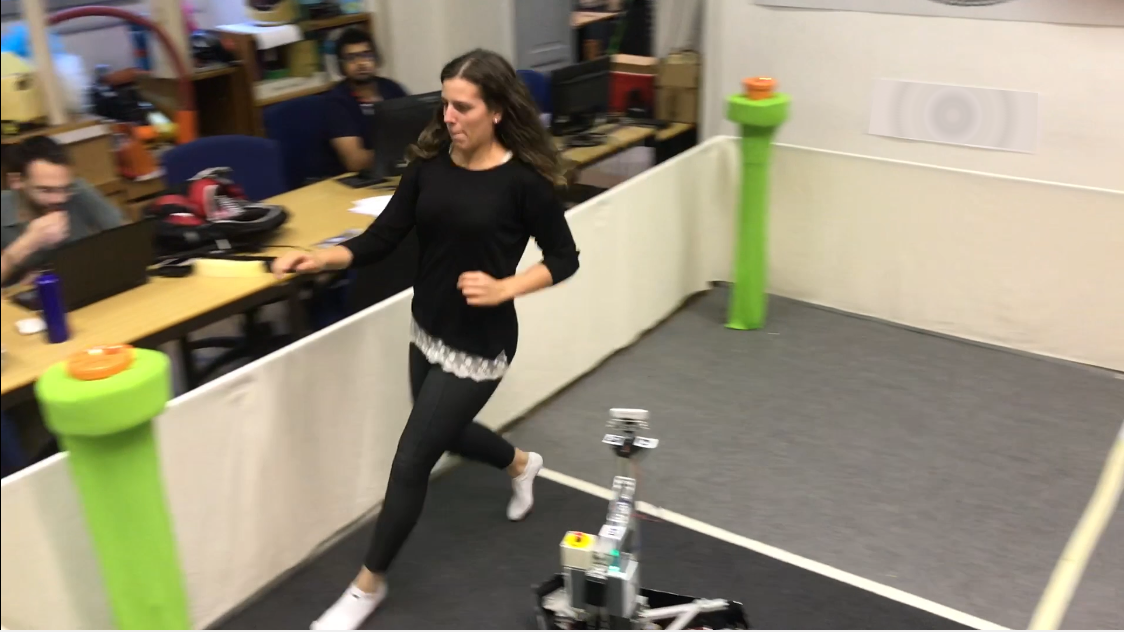
\includegraphics[width=0.5\columnwidth]{images/06-deception/frontPaper23}}
%\caption{Human-Robot interaction scene from our experiments.}
%\label{fig::front}
%\end{figure}

The main issues that should be faced in this field concern the robot's intelligence as perceived by the human player: low or too high levels may induce the player to leave because the robot is not considered as a valid competitor, and this lowers the entertainment level of the game. 

We are focusing on a challenging type of games, where the players are involved in a physical, quite demanding activity. This type of games has been introduced as~\gls{pirg}~\cite{martinoia_physically_2013}). In~\gls{pirg}s, it is important to model the player, by using the only available data that could describe well enough the movements of the player.

%=============================================
% Sommario
%---------------------------------------------
\selectlanguage{italian}
\chapter*{Sommario}

Scrivimi
\selectlanguage{english}

%=============================================
% Epigraph
%---------------------------------------------
\chapter*{}
\vspace*{\fill}
\renewcommand{\epigraphsize}{\large}
\setlength{\epigraphwidth}{0.5\textwidth}
\epigraph{\itshape True happiness is to enjoy the present, without anxious dependence upon the future, not to amuse ourselves with either hopes or fears but to rest satisfied with what we have, which is sufficient, for he that is so wants nothing. The greatest blessings of mankind are within us and within our reach. A wise man is content with his lot, whatever it may be, without wishing for what he has not.}{--- Seneca}
\cleardoublepage

% Dedication
\chapter*{}
\begin{flushright}
\null\vspace{\stretch{1}}
To the ones I bring in my mind and heart.
\vspace{\stretch{2}}\null
\end{flushright}
\cleardoublepage

%=============================================
% TOC
%---------------------------------------------
\tableofcontents
\listoffigures
\listoftables
\printglossaries
\cleardoublepage
\newpage

% Now let's go back to normal numbering
\setcounter{page}{1}
\pagenumbering{arabic}
\cleardoublepage

%=============================================
% Main document
%---------------------------------------------

\chapter{Introduction}
What seems to be a natural evolution for game playing experience is to bring the elimination of screens and devices in order to present the users with the possibility to physically interact with autonomous agents in their homes without the need to produce a virtual reality. This pretty new style of games has been recently defined as~\gls{pirg} and has as the main objective the exploitation of the real world (in both its dynamical unstructured and structured aspects) as environment and one or more real, physical, autonomous robots as game opponents or companions~\cite{martinoia_physically_2013}.

Like commercial virtual games, the main aspect of~\gls{pirg}s is to produce a sense of entertainment and pleasure that can be ``consumed'' by a large number of users\footnote{In this work, since the player is an user for the gaming application both words ``player(s)'' and ``user(s)'' will be used interchangeably.}. Furthermore, an important aspect of autonomous robots and systems during the game should be, as expected, an exhibition of rational behavior and, in this sense, they must be capable enough to play the role of opponents or teammates effectively, since by practical means people tend to avoid to play with or against a dull entity~\cite{martinoia_physically_2013}.
To come up with better agents it's easy to think about extracting knowledge from the behavior of co-players and implementing some mechanism for modeling them, in particular their preference for specific low-level actions and interaction patterns. Being able to recognize co-player's intention may substantially improve the capacity of taking better decisions about the actions to take.  At least in the human's perspective, this ability is critical since interpersonal interaction presupposes understanding  motivations and high-level plans, aas well as estimation of future events~\cite{sukthankar_plan_2014}.

When it comes to extract useful information from agent's behavior, one can see at least two main different, yet related, approaches: \begin{inparaenum}[\itshape a\upshape)]\item Modeling for competitive advantage and \item Modeling for experience optimization\end{inparaenum}. In the former, techniques for evaluating pay-offs from interaction patterns, such that provided from \textit{game theory}, play an important role not only to what concerns interactions with virtual agents, but real-world events involving humans as agents (e.g. trading, patrolling, competition) or physical robot entities. In order to get some competitive advantage against an adversary with private strategies and conflicting goals it is necessary to adapt to the dynamics of the situation caused by the game play~\cite{rofer_overview_2012}. In essence, this means that it is vital to pay attention to any information from the opponent's behavior that might help to optimize the decision making process and find appropriate countermeasures.

The focus on modeling behavior for experience optimization, is much related to the idea of extracting useful features from users in order to adjust parameters that are correlated with their experience in the activity, for the sake of offering a better product or helping the user to achieve some particular goals. In a gaming scenario, this notion is commonly applied when designers attempt to define a mechanism capable of adjusting the difficulty or general appearance of the game in the expectation of rising the player's entertainment. Very traditionally, the sense of game difficulty is designed to increase along the course of the experience, and it can either happen in a linear fashion or through steps represented by the levels or phases, where a player is forced to select the difficulty level through a set of discrete options (easy, medium, hard, very hard). However, given the observation that very often this ``static'' way of setting up a difficulty curve is not accurate enough and it may not account for the difference between players or even the different rates of leaning of each of them, in principle, it turns out useful and natural to think about coming up with modeling techniques that may empower the play experience. 

However, such models greatly depend on the type of scenario they are applied to. In a computer game scenario a computer-controlled agent receives noise-free sensory data, but this is not possible in a real-world scenario, especially in robotic applications such as~\gls{pirg}. 
%ANDY I really cannot understand the meaning of the enxt sentence. What solutions? Most computer games are quite well designed, and design is reflecetd in the implementation. ->The general suspicion about a full spread of such solutions, mainly in virtual game development, is that they ultimately take the control away from the design and put it basically in the code, which has obvious drawbacks, ranging from high-demand for computational resources and storage to general game behavior~\cite{hunicke_ai_2004}. 

In summary, it would be important to have an autonomous robot playing in a~\gls{pirg} and able to automatically adjust its behavior such that it may likely match the user's skill and, by doing so, could maintain the user engaged and entertained. Also, it is important to make thhis robot appear rational, possibly smart. 

In this thesis work, after providing a panorama of approaches that take inspiration from \textit{artificial intelligence} (AI) and \textit{machine learning} (ML) techniques in order to tackle the problem of modeling co-existing agent's behavior and activity in games and robots, we propose models and report of results showing effort in addressing the design of better agents for~\gls{pirg}.

The scope of this document is heavily centered on model proposals that can latently model player activities and general behavior.  %Next section details our objectives and research organization.

\section{Research questions, hypothesis and objectives}	
Since, in any kind of~\gls{pirg}, autonomous robot are supposed to be perceived as smart entities, the key point for investigation deals with finding good answers to two main questions:

\begin{itemize}
\item How to discover player types and quantify player behavior in~\gls{pirg}?
\item How it is possible to adapt the behavior of the robot to optimize the satisfaction of the human players?
\item To what extent does adaptation impact reported entertainment?
\end{itemize}

From this, the objective of this thesis focuses on the exploitation of~\gls{ml} techniques to the design of better~\gls{pirg} robotic agents, which should lead to more engaging playmates, possibly capable of performing behavior/strategy adjustment. The hypothesis is that~\gls{ml} would help to decrease predictability in robot behavior and introduce game dynamics capable of considerably empower the user’s engagement, making so that the agents can be well accepted as game companions. Specifically, the general goals were:

\begin{itemize}
\item To identify and devise~\gls{ml}-based techniques for player modeling to design~\gls{pirg} from the view of human-robot interaction. %ANDY I did not understand what you meant with this and my rewriting is a non-sense
\item To implement user's behavior modeling in~\gls{pirg} robots by reasoning about data coming from player tracking in the shortest possible time, as required by the~\gls{pirg} setting.
\item To explore ways of strategy adjustment using information about past interactions (player's typical behaviors, preferences, etc.).
\end{itemize}

It is supposed that autonomous and learning systems that encompass perception, action, and communication in a unified and principled way via~\gls{ml}-based techniques lay at the core of a new frontier for robotics, and~\gls{pirg}s in particular. 
We also aimed at keeping control on technical constraints  to enable the spread of~\gls{pirg} in the society, making them reach the market in large scale. In particular, we explored the use of cheap sensors, and algorithms requiring little power ("green algorithms") to be executed in real time and operating in non-structured environments, 

\section{Thesis outline}
The thesis is divided into the following chapters.

\begin{itemize}
\item\emph{Chapter~\ref{ch:art}:} Many approaches for tailoring %ANDY Actually, "tailoring" refers to adaptation, not to modeling. Do you plan to mention also the "modeling" approaches, isn't it?
game experience to players had been proposed over the years. The chapter presents an overview of such literature, placing~\gls{pirg} as a relatively new area of research.
\item\emph{Chapter~\ref{ch:foundation}:} The game environment and robot platform are at the core of a~\gls{pirg} application. In this chapter, we detail the designed environment and adopted robotic platform. Other mathematical background are provided.%ANDY what this last sentence mean? WHat kind of background on what? Please detail. I wouldn't mix mathematical details with the game description.Let's keep them in separate chapters.
\item\emph{Chapter~\ref{ch:activity}:} One step towards allowing effective player modeling is the implementation of an activity recognition system. In this chapter we describe the efforts on exploiting a simple input data transformation for the recognition of motion primitives in acceleration patterns akin to archetypal activities in the game scenario.
\item\emph{Chapter~\ref{ch:modeling}:} Player behavior modeling is the backbone of adaptive behavior strategy for playing robots. The chapter presents a new proposal for latent player behavior modeling.
\item\emph{Chapter~\ref{ch:adaptation}:} Adaption is by no means a trivial task specially in the context of~\gls{pirg}. In this chapter, we detail a system to actively select game parameters appropriate for the specific human player.
\item\emph{Chapter~\ref{ch:deception}:} Engagement is believed to be related to several factors and one of such is the level of information about the opponent actions. In this chapter, we present a study case of the use of deceptive motion during play. Results indicate that on our particular game scenario the human capacity to correctly identify the robot deceptive intentions is blurred possibly by the intensive cognitive load demanded by the activity.
\item\emph{Chapter~\ref{ch:key}:} The design of~\gls{pirg} is an intensive process. In this chapter we provide some key-issues regarding how one may develop successful engaging experiences.
\item\emph{Chapter~\ref{ch:future}:} Concludes the thesis and details further direction for our research.
\end{itemize}

\section{Paper contributions}
\begin{itemize}
\item \fullcite{oliveira_learning_2018}
\item \fullcite{oliveira_modeling_2017}
\item \fullcite{oliveira_activity_2017}
\end{itemize}

\chapter{Physically interactive robogames}\label{ch:art}
\epigraph{\itshape Begin at the beginning, the King said gravely, ``and go on till you come to the end: then stop.''}{---Lewis Carroll, \textit{Alice in Wonderland}}

\section{Definition}
Since more than 10 years, video games companies operating in the mass market of entertainment have aimed at establishing a new paradigm that involve the players actively moving in front of the screen, actually interacting with the game in a three-dimensional virtual or augmented space. This often happens by constructing an immersive virtual reality game where players are plunged in an artificial world reproduced by \textit{ad-hoc} intelligent systems devices~\citep{zyda_visual_2005}. This scenario, although enabling impressive game experience often requires to wear special devices that may limit the quality of the movement possibilities~\citep{martinoia_physically_2013}.

Enabled by the increased maturity of fields like social robotics, artificial intelligence and machine learning, \cite{martinoia_physically_2013} pushes forward the idea of designing a new level of game experience: that of~\glsdesc{pirg}. They provide a definition of~\gls{pirg} adopted in this work:

``\textit{A Physically Interactive RoboGame consists of a number of autonomous agents (including software, hardware, and physical agents) of which at least one is an autonomous robot, and one is a person. These agents interact with each other in a possibly variable and unknown environment, by following some game rules, so that the human players can have fun}~\citep{martinoia_physically_2013}.''

The authors also emphasize the existence of similar attempts for presenting robots as games where, in most cases, robots act more or less as mobile pets (e.g., \cite{fujita_open_1997,shibata_emotional_1996}). In this case, interaction is often seen as limited to almost static positions, not exploiting rich movement, nor high autonomy; the credibility of these toys to really engage lively people, such as kids, cannot be high. A notable exception is Kiro~\citep{weigel_kiro-table_2005}, a robot able to successfully play table soccer even with experienced users. In the game, the movement is limited to the control of the table bars, and the game is the robotic version of a classical bar game. The interaction provided by Kiro is relatively simple, in a very structured situation, but despite of this it matches exactly the user's expectations~\citep{martinoia_physically_2013}.

Robot toys are presently the largest amount of robots delivered in our homes, at a rate of millions every year. In almost all the cases, the interaction is limited to stimulus-response reactions, but the introduction of low-cost sensors and computer power are making it possible to introduce a richer interaction and games specifically designed for mobile robots. In this direction, a company called~\href{https://anki.com/en-us}{Anki} started to make use of artificial intelligence techniques for the task of bringing consumer robotics into physically gaming experience. During the keynote event at Apple's Worldwide Developers Conference in 2013, the company revealed its first product: Anki Drive, a racing game featuring toy-size robotic cars controlled by a mobile app that serves as an~\gls{ai} engine. In 2015, the product was considered one of the best toys available in the market, which somehow expressed the interest for this kind of real-world smart robotic game experience. In the game set, the Anki Drive cars sense their positions on a carpet-like track and continually exchanging data via Bluetooth with the mobile phone. The app computes possible actions and decides what each car should do based on its objective. Thus, because is the app that defines how each car behaves and creates different gameplay scenarios, the cars can have different ``personalities'' and get customized features. Despite of the app ability for orchestrating the behaviors of the cars and posit a sense of autonomous driving, players are still limited to the use of their mobile to actually drive the cars, racing against each other or taking on the~\gls{ai} (facing other cars). Players are not directly involved in physical interaction with the robot, and play a kind of \textit{indirect} \gls{pirg} through a mechanical device used as a kind of avatar representing the players themselves. Anki has recently expanded its market by launching a new robotic toy, Cozmo, an intelligent robot that is able to interact and play games with users.

In a~\gls{pirg}, however, physical autonomous (often mobile) agents are actively engaged in a game that creates some sort of interaction, either competitive or cooperative, between humans and robots, moving in the physical world. Robogames will be one of the next robotic products for the mass technological market, thus demanding a large exploration of new methodologies and applications, especially for what concerns methods for enabling high autonomy, intelligence, and adaptive behavior, in order to respond to demands in engagement support like the ones expressed in~\cite{yannakakis_how_2008} and ~\cite{yannakakis_entertainment_2008,yannakakis_real-time_2009}. 

Since some years, a set of~\gls{pirg}s have been developed and tested at the Artificial Intelligence and Robotics Laboratory (Politecnico di Milano, Italy), focusing on a more direct, physical interaction with players, as defined in~\cite{martinoia_physically_2013}. As an example, the Jedi Trainer 3.0 (see figure~\ref{fig:jedi_trainer}) was developed with the goal of resembling a scene of the first Star Wars saga movie ``Episode IV - A New Hope''. The game was designed to use an autonomous drone, a Parrot quadricopter, flying around the human player (Jedi trainee) and shooting at appropriate time by making a sound recalling the shot of a laser blast. The drone always aims at shooting at the ``Jedi trainee'' (human player) chest that in turn physically interact with it using a light-saber-looking object trying to parry the drone attack. The Jedi Trainer has been successfully tested in different unstructured environments, as reported in~\cite{bonarini_timing_2014} and~\cite{martinoia_physically_2013}.

\begin{figure}[h]
  \centering  
  \framebox{\parbox{6cm}{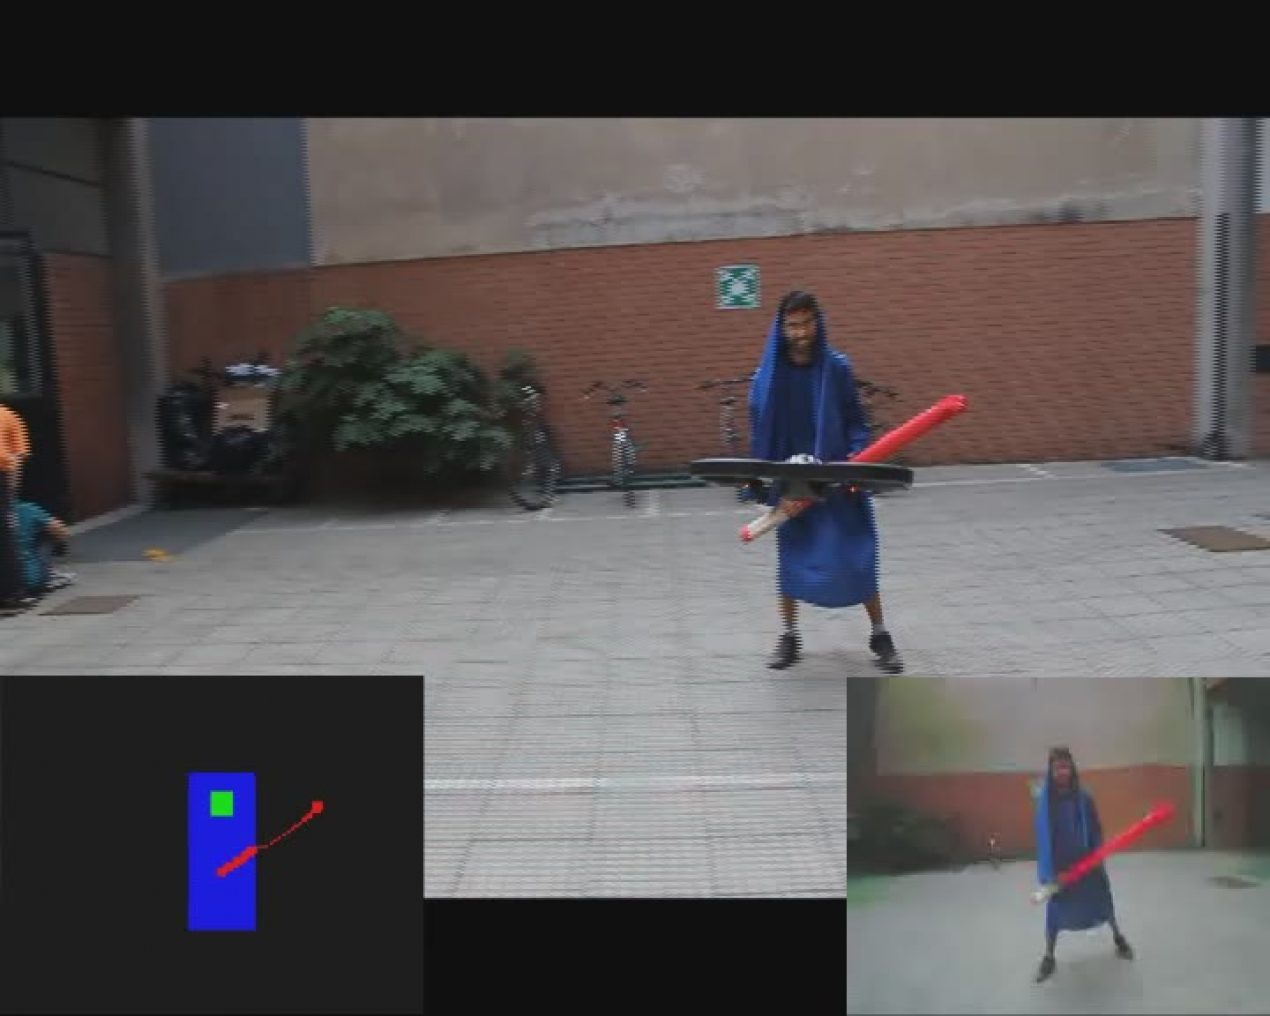
\includegraphics[ width=6cm]{images/02-art/jedi_trainer}}}
  \caption{The drone and the Jedi trainee playing JediTrainer 3.0. On the bottom right the image taken by the on board camera, on the bottom left the interpretation of the image in terms of color blobs. The green rectangle on the top of the blue one is the target where the drone is aimed at blast its laser shot~\citep{bonarini_timing_2014}.}
  \label{fig:jedi_trainer}
\end{figure}

Another example is RoboTower. It is inspired by the videogame Rock of Ages. In the game, a 30 cm high robot has to bring down a set of towers in three minutes. Human players can interact with the robot by delaying its movement through the use of cards. These cards are selected from a deck they have in their hands and put in front of the robot, which can read them when it passes over. Each card represents either an action that the robot has to execute (go back, turn around) or a deficit for its sensors (go blind), or a stop for an amount of time. A red tower correspond to the player's home and when ruined he loses; other towers are production plants that are used to recharge the delaying cards, and make them again playable after a given time proportional to the number of active plants (Fig.~\ref{fig:robo_tower}).

\begin{figure}[htp]
  \centering  
  \framebox{\parbox{4cm}{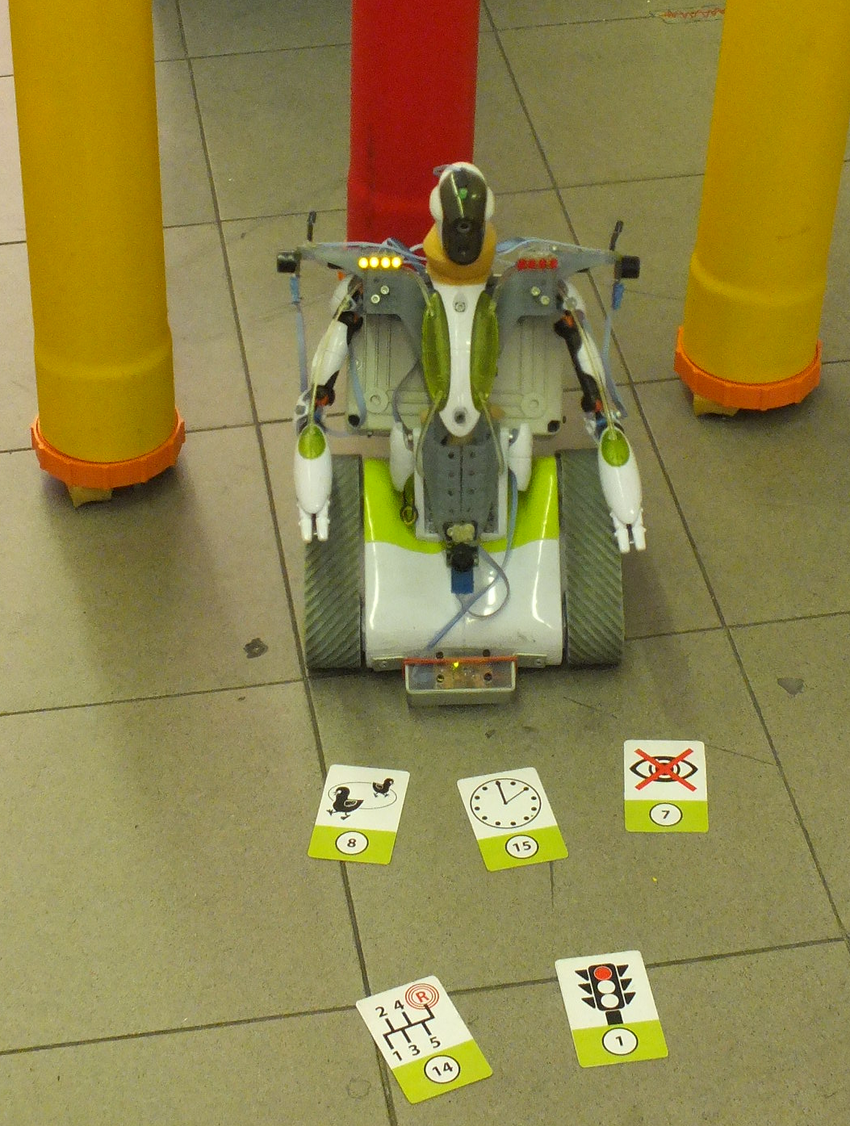
\includegraphics[width=4cm]{images/02-art/robotower}}}
  \caption{A view of the robot, the cards and the towers used in the RoboTower~\citep{bonarini_timing_2014}.}
    \label{fig:robo_tower}
\end{figure}

There are also some example of~\gls{pirg}s designed to play with children with special needs. An example of such is Queball~\citep{salter_designing_2014}, a robotic ball proposed to engage autistic children in games that could have therapeutic goals. Teo~\citep{bonarini_huggable_2016}, in turn, is a huggable, mobile robot designed to play games with autistic children, and to provide the possibility to make free play as well as structured play experiences.

Being able to evaluate how people play is crucial for an adaptive game. In the virtual game industry, several studies have been published, most of them using artificial intelligence and machine learning algorithms. For instance,~\cite{drachen_player_2009} reports about emergent self-organizing maps for grouping types of players. An approach based on genetic algorithms for capturing and modeling individual entertainment is given in~\cite{yannakakis_entertainment_2008}, where the main goal is to construct a player model, in this case a child playing a Playware game. ``Playware is the use of intelligent technology to create the kind of leisure activity we normally label play''~\citep{lund_playware_2005}. The system can predict the answers to a question asking which variants of the game are more or less ``fun''. In that work, the model is constructed from physiological signals measured during play. 

As it can be easily deduced, the new application field of~\gls{pirg} and the complexity it requires prompts for a new endeavor of~\gls{hri} which is defined as the study of how humans can interact with robots, ``and how best to design and implement robot systems capable of accomplishing interactive tasks in human environments''~\citep{feil-seifer_human_2009}. Undoubtedly, robogames appears as an interesting application to investigate~\gls{hri} issues as their design process has to do not only with the technical issues of a robotic application, but it has also to consider other important aspects, including playability and usability of the game~\citep{martinoia_physically_2013} as well as user engagement and entertainment.

The necessity of investing on the research and implementation of intelligent algorithms becomes more and more evident as a way to improve~\gls{pirg} design and help to popularize the idea of having such products on the market. In particular it is important to investigate how to develop appropriate cognitive abilities in autonomous robots by the use of machine learning (ML) techniques. One example of such ability would be  intention detection for strategy adjustment. 

Also, it is important to focus on the exploration of mobile robot bases with cheap sensors and algorithms requiring little power to be executed in real time (``green algorithms") in non-structured environments, since these are constraints currently addressed in robogames, and in the whole Robotics community, in order to make robots reach a wide market. 

Properly exploiting cognitive abilities in robogames may increase the player's engagement since any apparently rational behavior of the robot may bring to accept it as a robotic companion (or opponent) ``while random actions or too complex strategies for the cognitive or perception levels of the players are perceived as not purposeful''~\citep{martinoia_physically_2013}. Due to the inherent complexity involved in the typical scenario, it is not possible to entirely rely on ``hard-coded'' abilities that are static across time and once learned by the human player tend to decrease interest. The problem of designing new interesting~\gls{pirg}s calls for the massive use of~\gls{ml}-based techniques to make sense of the obtained interaction information, thus presenting itself a new field of research.

\section{Overall design guidelines}\label{sec:dimensions}
From our experience, we have identified at least three dimension in which one must pay attention to when designing a new~\gls{pirg}. Each dimension presents its own set of utilities/challengers some of which are summarized in Figure~\ref{graph:PIRG_design_structure}. 


\begin{figure}[h]
    \centering
    \def\homomorphism{(0,0) ellipse (6.0cm and 3.5cm)}
    \def\isomorphism{(-2,0) ellipse (4.0cm and 2.5cm)}
    \def\endomorphism{(-4,0) ellipse (2.0cm and 1.5cm)}
    \begin{tikzpicture}
      \begin{scope}[fill opacity=0.1]
        \fill[magenta] \homomorphism;
      \end{scope}

      \begin{scope}[fill opacity=0.5]
        \fill[cyan] \endomorphism;
      \end{scope}

      \begin{scope}[fill opacity=0.5]
        \fill[orange] \isomorphism;
      \end{scope}

      \draw \homomorphism;
      \draw \isomorphism;
      \draw \endomorphism;

      {
        \scalefont{2.0}
        \node[text=black] at (-4,0) {Hardware};
      }

      {
        \scalefont{1.5}
        \node[text=black, align=center] at (0, 0) {Playing for\\competitive\\advantage};
      }
      
      {
        \scalefont{0.5}
        \node[text=black, align=center] at (-4, 1) {Power Consumption};
        \node[text=black, align=center] at (-4, -1) {Kinematics};
        \node[text=black, align=center] at (-3.5, 0.5) {Sensing};
        \node[text=black, align=center] at (-3.5, -0.5) {Robustness};
      }
      
      {
        \scalefont{0.9}
        \node[text=black, align=center] at (-1, 1.3) {Planning};
        \node[text=black, align=center] at (-2, 1.9) {Opponent tracking};
        \node[text=black, align=center] at (-1, -1.3) {SLAM};
        \node[text=black, align=center] at (-2, -1.9) {World modeling};
      }
      
      {
        \scalefont{0.9}
        \node[text=black, align=center] at (2, 2.3) {Clustering};
        \node[text=black, align=center] at (3.5, 1.5) {Skill modeling};
        \node[text=black, align=center] at (2, -2.3) {Deception};
        \node[text=black, align=center] at (3.5, -1.5) {Optimization};
      }

      {
        \scalefont{1.5}
        \node[text=black, , align=center] at (4, 0) {Playing for\\entertainment\\ optimization};
      }
    %   \node[align=left] at (  -2, 2) {Auto-\\morphismen};
    \end{tikzpicture}
    \caption{The general design dimensions for a robot in~\gls{pirg} environment. The \textit{hardware} dimension is central to a~\gls{pirg} application and are the ones from which the overall robot behavior is constrained to. The \textit{playing for competitive advantage} collects the systems for planning actions towards winning the game, i.e., play competitively. \textit{Playing for entertainment optimization}, instead, defines the mechanisms from which the robot regulates its competitive capabilities towards making the player more engaged. This last dimension encompasses~\glsdesc{dda} approaches.}
    \label{graph:PIRG_design_structure}
\end{figure}

The three basic dimensions (or problems) of interest in Figure~\ref{graph:PIRG_design_structure} are related to the specific capabilities of a mobile robot to achieve a suitable in-game performance. We delineate such dimensions as follows:

\begin{itemize}[leftmargin=*,labelsep=5.8mm]
%TODO These  should have the same names as those in the figure and also the same components should be mentioned and introduced. What is described here below should be rewritten in much more consistent way. The first level cannot be only HW, but also the basic control and sensing capabilities, as well as the game rules and corresponding environment. 
\item \textbf{Hardware}: This dimension is supposed to collect the hardware aspects of the robotic platform, such as sensing, power consumption, structure robustness, kinematics, computing power. As to what regard sensing, one must be concerned with the capacity to understand the world around while obeying the game rules given a particular choice of sensors. In~\gls{pirg}, the choice of sensors has a considerable monetary impact as well as an impact in the robot's capacity to play, thus, it should be done carefully. Power consumption, in turn, direct impact the time of interaction as it supports the entire robot activity. Robustness refers to the chassis and physical appearance of the robot. Decisions about this aspect must  take into consideration the material stress and other related concepts that the platform is required to suffer while playing. This also includes safety issues that the designer must be aware of. For instance, the design must consider whether or not collisions among players (human and robot(s)) are possible and whether such collisions offer risks to their physical safety. 

Kinematics is one of the most important aspects of this dimension of design since it guides the ability of the robot to offer a good level of challenge when playing. It is an aspect most related to the role of the robotic player in the game and must be defined in relation to the game rules and other players' role. 

Additionally,  an aspect of importance related to hardware is the case of in-game elements that are external to the robot themselves. Although external, they have a specific role in the game interaction as a whole and their existence are conditioned to the game rules. An example of such elements are the cards and towers in RoboTower~\citep{bonarini_timing_2014} and towers in RoboTower v2~\citep{oliveira_activity_2017}. Despite such elements being external to the robot, one must deal with their operability and functionalities, how it communicates with other game entities as well as how the robot and humans interact with them.

Perhaps, the most important of all hardware issues is whether or not the robot has enough computing power to support a good interaction. It is so, because computing power connects the performance of the platform in other concepts, such as sensing, navigation and planning, and energy consumption. In general, each~\gls{pirg} is unique in terms of hardware demands, but such demands are at the first level of design and must be chosen carefully so as to support all interaction. Choosing the right hardware for a~\gls{pirg} is a time consuming process estimated to have a bidirectional relationship with the game rules and the attribution of roles to players.

\item \textbf{Playing for competitive advantage}: In-game competitive capabilities, which are more related to the intelligent selection of actions aimed at achieving in-game goals. In other words, this dimension captures the intricacies of planning and rational behavior, using the hardware available. The ability to self localise (~\gls{slam}), locate other players, represent game states, and act consistently is a sub-component of planning, while the ability to navigate guaranties the planned sequence of actions is executed well. For planning, a vast literature of general methods is available to the designer and the responsibility is often concentrated at the definition of performance measures to ensure rationality in the selection of a plan. The great majority of methods rely on the fundamental principle of~\gls{meu} following the direction of classical problem-solving agent architectures~\citep{russell_artificial_2009}.

In the dimension of playing for competitive advantage, opponent tracking is a required component since it is necessary to the system monitor the player activity and act accordingly. As it is going to be exposed later, the existence of an explicit game activity player model in this dimension is facultative. This is because it is possible to design agents that are able to effectively play while maintaining only a minimal general (non game-related) model of the player, such as mathematical position filtering models using bayesian filters (\eg Adaptive Monte Carlo Methods, Kalman Filter, etc). As an example, the player tracking model we have used in our experiments~\ref{sec:player_tracking} is a generic mathematical model which estimates the player's position as a particle in space. 

Naturally, player models that try to picture players from their in-game actions and attributes can also be considered in this phase of development. Such player models would keep a record of the standard player behavior and use that so as to take advantage and increase the chances of winning the game. It has a different purpose of player behavior modeling for entertainment maximization, as it will be said next. Player modeling to support competition can be viewed as a base component to modeling for entertainment maximization. This last is the central point of interest in~\gls{pirg} applications.

\item \textbf{Playing for entertainment optimization}: This dimension cover the adaptive power of the playing agent, which is a higher level dimension concerned with how and when to adjust the robot performance to match that of the current player. 

This dimension is also suppose to include mechanisms for~\gls{dda}, which goal is to design a system (a game) that can match the difficulty to that of the player.~\gls{ml}-based techniques, such as clustering, optimization, latent skill modeling can be used to extract useful information from players. Another interesting attribute of behavior explored in this design dimension is the use of social interaction and the use of deception as a mean to introduce dynamic behavior in robots and understand its impact to fun (we exploit deception in chapter~\ref{ch:deception}).

In general, this design dimension must broadly incorporate aspects for modeling and acting towards supporting entertainment. The main focus by this dimension is not playing to win, but to control the capabilities of winning the game (in the second dimension described above), \ie the difficulty and/or other aspects of play, towards engaging the player. Player modeling in this dimension is concerned with achieving this goal and are likely to include, as sub-component, player models for increasing competition.
\end{itemize}

The third dimension, organically based on the two other, defines constraints on the robot behavior such that the action selection is no longer just governed by the tendency to be competitive/helpful, but it is also driven by the compelling necessity to support the player interaction, in real time, as robustly as possible. Although not essential for the second dimension, player behavior modeling techniques are an essential for the third one. Such techniques are intended to account for the player usual behavior, thus, being useful for improving platform behavior. It is in this aspect of modeling that we concentrated most of our work, as it is going to be clear from chapter~\ref{ch:modeling}.

Additional to the general dimensions mentioned above,~\cite{bonarini_timing_2014} presented key aspects on timing issues observed during the design of several robogames, some of which related to the structure of the game:

\begin{itemize}
\item \textbf{Duration of the game}: This is a key-point since a game should reach its end in a time that guarantees to keep the players involved and to make them enjoy it. This greatly depends on the activity to be performed. In the~\gls{pirg} case, the user's physical activity, i.e the workload, is the core of the interaction and it must be taken into account when defining the game duration so that the player can come to the end with a proper fatigue requirement. The reader is invited to think about the effect on engagement when this point is not well designed.

\item \textbf{Duration of an in-game task}: In a game, a set of tasks should be achieved. Naturally, the duration of such tasks has to be bounded by the duration of the game, or a game match. So, the duration of in-game tasks can be appropriately defined in order to provide some pressure on the players such that it may be likely to engage them, rise their interest, since an appropriate level of pressure and anxiety is related to challenge. The take-away idea here is that limiting the time available for an in-game task is a key-point to make it challenging.

\item \textbf{Duration of non-interactive activities}: In some games, there are activities that must be performed by a single player and so must have the right amount of time dedicated to them, i.e, a right period of time without any interaction with others (e.g, a solution of a problem, a recovering procedure). If these activities have to be done by human players, enough time has to be left for their accomplishment, but not too much time that could make them less challenging. On the other hand, if these activities must be performed by the robot(s), the human player should somehow be involved at the same time in some other activity, or the time dedicated to them should be short enough in order to lower the likelihood of making the human player bored, but long enough to be credible w.r.t. the storyboard of the game.
\end{itemize}

Some timing aspects related to the performance of both the human players and robot were also mentioned in~\cite{bonarini_timing_2014}.

\begin{itemize}
\item \textbf{Reaction time}: The time each player needs to react to an external event can be a constraint to be considered in game design. The human player's reactions in a physical interaction can be instinctive, thus requiring few hundreds of milliseconds to be activated, or may require some cognitive activity (e.g., reasoning, recognition), whose duration may span also some seconds. In~\gls{pirg}s, since they are often designed for a lively interaction, the cognitive load is usually relatively small, and a time around one-two seconds for a cognitive response from the human player in a challenging situation is often considered as appropriate. The reaction time of the robot player mainly depends on the time to recognize a situation, which is related to the time required to elaborate signals, which in turn depends on the complexity of the data to be analyzed and on the available computational power. Since~\gls{pirg}s are targeted in principle at a mass market comparable to the one of video games, the robots should be low cost, with simple sensors, and the available computational power might be as low as the one provided by cheap processing systems, like Arduino or Raspberry PI, up to that of an external laptop, tablet or smart phone. This might be a time constraint to be considered in game design, possibly justifying the related delays in the story.

\item \textbf{Actuation time}: Also actuation time may concern both the human and the robot player. For people, they might be constrained by some devices to dedicate time to perform an action (e.g., to perform a gesture with a WIIMote device). This might be desired to put some challenge in the game, and also to reduce the power of the human player w.r.t. that of the robot, so to make the game more even. For the robot, the actuation time might be a constraint given by the selected mechanical implementation, or might even be desired to reduce the power of the robot. For instance, if a robot could run fast enough to reach a target before a human player, it might be the case to reduce its speed so that the player can compete with it with some possibility to win.
\end{itemize}

Some other timing aspects are related to the establishment of a relationship.

\begin{itemize}
\item \textbf{Opponent behavior detection time}: Playing with artificial entities is engaging if the human player forgets the status of the opponent and attribute to it some human-like abilities. In particular, human players would like to play with entities that show some intelligence and intentionality. A way to achieve this status is to understand why the entity is performing an action, and, in general, what is its behavior, and what it aimed at. This may require an amount of cognitive activity proportional to the complexity of the behavior. In the mentioned experiments turned out that a random behavior is perceived as not interesting: the player believes that it is not worth to spend time with a silly entity. A too complex behavior is perceived as a random one, mostly because in~\gls{pirg}s there is not much time to reason in a cool way on all the aspects of the perceived actions. A good behavior is one that requires a short time to be detected: not too short to consider the robot as ``too simple minded'' to play with, but also not too long to dismiss the cognitive activity of trying to understand it while the player is confronting the robot.

\item \textbf{Credibility}: Each action should have a motivation, and should be credible w.r.t. the perceived motivation. Timing of the action should be consistent with this. For instance, if the robot seems to take a decision about what to do, the consequent action should last until there is a good motivation to change it. For instance, if a autonomous robot would change its movement direction randomly, there would be no apparent reason to motivate the change, and the robot would be perceived as silly. This, of course, depends on the~\gls{pirg}. In Jedi Trainer 3.0, for example, a random decision about the direction to take is consistent with what the robot is doing: trying to find a gap in the trainee guard.

\item \textbf{Activity pace}: Each player is assumed to do actions with a purpose for the game. Since they are interacting, the activity pace should be similar: a different pace, a different time between the selection of subsequent actions, would be perceived as if one would be favored w.r.t. the other one. Uneven games, in one sense or the other, are usually not appreciated.

\item \textbf{Timing perception}: In interaction, timing is a subjective perception, and it can be modified by the interaction mood, or media, or by external devices. If there is an exchange, its pace can be modified by a ``modeling and lead'' strategy. If there is a time limit to perform a task, the perception of its urgency might be further increased by taking a faster pace in all movement changes, or also by simply giving relevance to the time-to-end, e.g., by adding rhythmic lights, sounds, or clocks.
\end{itemize}

\section{Considerations}

This chapter is aimed at the presentation of relevant aspects and popular papers in the field of player modeling both to the extent of maximizing competitive advantage (section~\ref{compadvantage}) and experience optimization (section~\ref{ch:review_playing_optimization}). Despite the fact it is not supposed to be an exhaustive review of literature (for which the reader may refer to papers mentioned in section~\ref{reviews}), it was enough to spot interesting aspects one must consider when trying to achieve similar goals on~\gls{pirg}s. The motivation for this chapter was that of providing some insights, based on related literature, that might support the design of adaptive behavior in~\gls{pirg}s. 


\part{Platform design}

\chapter{Hardware}\label{ch:foundation}
\epigraph{For the things we have to learn before we can do them, we learn by doing them.}{--- Aristotle, The Nicomachean Ethics}
\section{Game environment}\label{sec:game_environment}
As mentioned in section~\ref{sec:research_question}, we were interested in understanding phenomena related to player engagement in~\gls{pirg}s with a mobile adversarial robot. For that, we had chosen to use RoboTower~\citep{bonarini_timing_2014} as a starting point, perfecting the interaction and playability.

A main difference concerns the playground, which in our case consisted of a rectangular area of 4m$\times$4m, and the extinction of cards as mean of interaction. Here, we used the player's proximity instead as interaction channel. On each corner of the playground, tubes (henceforth called ``towers'') were placed (details in figure~\ref{fig:towers}). Each tower was equipped with a button (which sits on the tower's cap) and four~\gls{led}s that could be progressively turned on, one by one.  Each~\gls{led} required the button to be pressed for 2.5 seconds, meaning that the tower took about 10 seconds of button push in order to light up all of its four~\gls{led}s.

The~\gls{led}s are supposed to display the progress of the human player in capturing a specific tower. For a given tower, after turning on all~\gls{led}s, it is said that the player had captured it. When a tower is secured, the robot cannot aim at it anymore.
Button pressing time was cumulative and could be distributed on different moments -- that meant that the player would not lose his progress if he stopped pressing the button before the tower is completely captured. 

The game mechanics and winning conditions were simple enough to allow for a large number of individual playing the game. In order to win, the human players must be able to secure all the existing towers without letting a single one be knocked down by the robot. If, at anytime, a tower falls (because of the robot or the player) the game ends and the human player loses. 

The robot was able to move across the entire playground just as the human player could and it was only constrained by the fact that an already captured tower, or one whose button is currently being pressed by the player, cannot be teared down. As main interaction channel between the two players,\ie robot and human, the human player could block the robot path at any moment by staying in front of it, causing the later to likely change target tower. Therefore, as consequence of the defined rules, while the player was trying to capture a given tower, the robot could try to tear down any other one.

%ANDY This would go in the robot description -> By relying on the lasers scans the robot can perceive its environment, locate itself and the human player during the game, being able to perform obstacle avoidance when appropriated.

The game definition in itself is no trivial task and it is, for the case of~\gls{pirg}, limited by the constraints imposed by the mechanical platform,~\ie the robot. Other than playability and fun, safety is also an important aspect and one that impose heavy bounds to the motion of the robot: a too fast of a robot would reduce the perception of the robot been safe too play against, thus limit the interaction. Experimentally, we have evaluated that a robot with a maximum linear speed of 1.4 m/sec would be too difficulty to play against and/or invincible (which is not the behavior we were looking for). Intuitively, as we allowed an increase in speed, an impact in difficulty would be perceive. Moreover, for a mobile robot as ours, speed have some negative impact in the robot control itself, through mechanical phenomena like wheel slippage, initial control, manoeuvrability, and navigation issues (localization and obstacle avoidance). Details about the robot platform is given in section~\ref{sec:roboplat}.

In summary, our game, called RoboTower v2, was designed such that we could have an environment rich enough to physically engage human players while allowing for the study of adaptive approaches towards supporting such engagement. RoboTower v2 stimulates player to maintain strong cognitive tasks, like: trajectory planning, attention and spatial reasoning and places itself as an interesting environment from which one could test~\gls{ml} approaches. Next we briefly detail the Towers used in the game in term of their properties and operating system.
%ANDY Here is one of the places were the smartness of game design has to be put in evidence.

%\begin{figure}[H]
%	\centering
%	\begin{subfigure}[b]{0.4\textwidth}
%		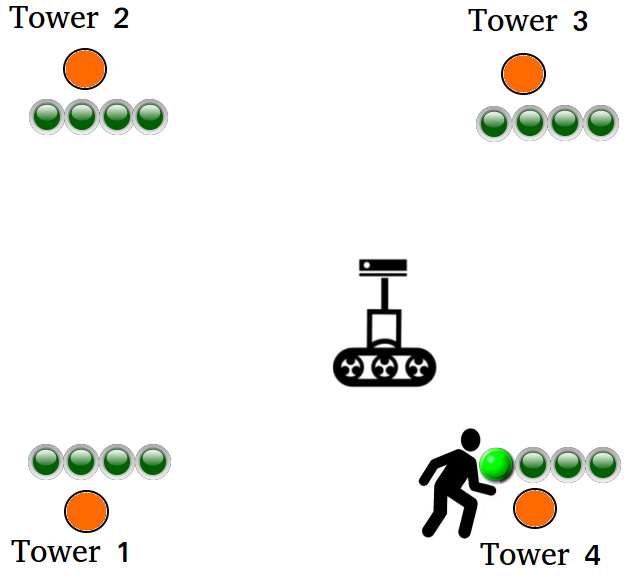
\includegraphics[width=5cm]{Chapter4/Figs/situation1}
%		\caption{Initial situation: player is capturing Tower-4}
%		\label{situation1} 
%	\end{subfigure}
%	\begin{subfigure}[b]{0.4\textwidth}
%		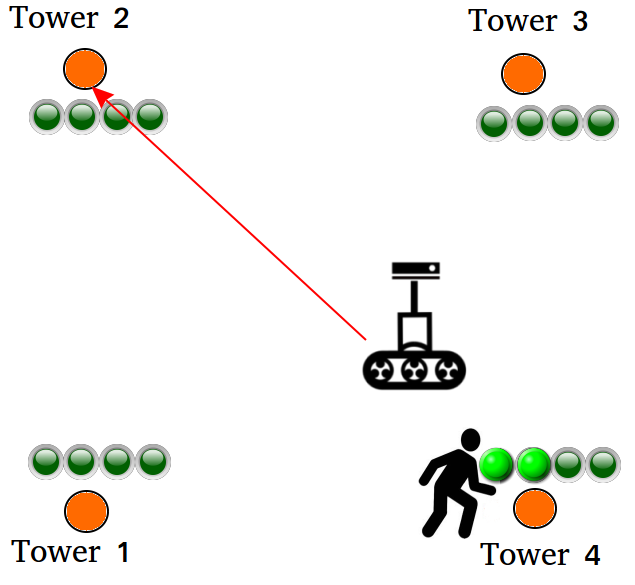
\includegraphics[width=5cm]{Chapter4/Figs/situation2}
%		\caption{Robot start moving in order to attack and tear down Tower-2}
%		\label{situation2}
%	\end{subfigure}
%	\begin{subfigure}[b]{0.4\textwidth}
%		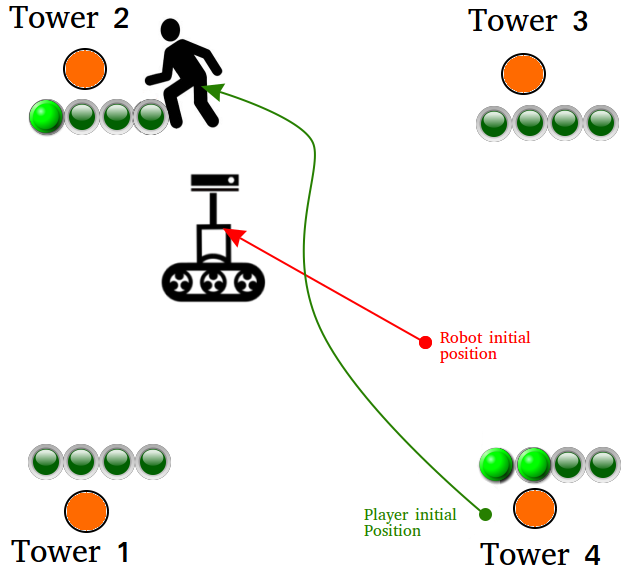
\includegraphics[width=5cm]{Chapter4/Figs/situation3}
%		\caption{Human player defends and start capturing Tower-2} 
%		\label{situation3}
%	\end{subfigure}
%	\begin{subfigure}[b]{0.4\textwidth}\centering
%		\includegraphics[width=3cm]{Chapter4/Figs/tubes}
%		\caption{Real towers that are used during the game}
%		\label{tubes} 
%	\end{subfigure}
%	\rule{35em}{0.5pt}
%	\caption{Schematic representation of the game:}
%	\label{overallgame}
%\end{figure}
%\begin{itemize}
%	\item figure~\ref{situation1}: The player is capturing the tower, when all the four LEDs are lit on the tower.
%	\item figure~\ref{situation2}: The robot attacks a Tower, it cannot try to tear down the tower that is currently being captured by the player.
%	\item figure~\ref{situation3}: The player stops the action of the robot by blocking its trajectory and defending the attacked tower. \textit{Please notice} how the progress on Tower-4 is not lost even if the player dismiss capturing it.
%\end{itemize}

%\begin{figure}[H]
%	\centering
%	\includegraphics[width=10cm]{Chapter5/Figs/im1}
%	\rule{35em}{0.5pt}
%	\caption{Moving robot tracking the movements of a human.}
%	\label{trackingconcept1} 
%\end{figure}

%To obtain the data from the human player that are needed to perform the tracking we used the Microsoft Kinect presented in~\ref{kinectsec} and a computer vision algorithm for blob detection previously integrated in the ROS environment using OpenCV libraries.

\section{Towers}\label{sec:towers}
Each tower was powered individually, being capable of transmitting its status to the robot at a constant rate. The circuit used the~\href{https://einstronic.com/wp-content/uploads/2017/06/NodeMCU-ESP8266-ESP-12E-Catalogue.pdf}{NodeMCU V3 ESP8266 ESP-12E} WiFi module\footnote{\url{https://goo.gl/TzAjwi} accessed on December 17th, 2018.} (see figure~\ref{fig:tower_electronics}) whose connection was done via a private network. The communication between towers and the robot was supported through~\gls{tcp} using the rosserial\_server\footnote{\url{http://wiki.ros.org/rosserial_server} accessed on December 17th, 2018.} package. Appendix~\ref{app:hard_appendix} provides additional hardware details for the towers. 

As power supply, a $7.4$V LiPo battery was used on each tower as can been seen on figure~\ref{fig:tower_electronics}. The nominal voltage for the boards was $5$V, which is supplied through a voltage regulator. A tilt sensor allows for the detection of fallen towers. A schematic of the circuit developed to detect such event is provided in figure~\ref{fig:tilt_circuit}.

\begin{figure}[h]
  \centering
  \begin{subfigure}[b]{0.3\textwidth}
  	\centering
    \framebox{\parbox{3cm}{\includegraphics[width=3cm, height=4cm]{images/03-foundation/cap1}}}
	\caption{}
	\label{fig:tower_cap_top}
  \end{subfigure}
  ~ 
  \begin{subfigure}[b]{0.3\textwidth}
  	\centering
    \framebox{\parbox{3cm}{\includegraphics[width=3cm, height=4cm]{images/03-foundation/cap2}}}
	\caption{}
	\label{fig:tower_electronics}
  \end{subfigure}
  ~
   \begin{subfigure}[b]{0.3\textwidth}
	  \centering
      \framebox{\parbox{3cm}{\includegraphics[width=3cm,  height=4cm]{images/04-activity/tubes.jpg}}}
      \caption{}
    \end{subfigure}
  \caption{a) Tower cap containing the button (red square) and \gls{led}s; b) Tower cap electronic; c) The four towers used in the game (height 110cm).}
  \label{fig:towers}
\end{figure}

\section{The robotic platform}\label{sec:roboplat} 
As depicted in figure~\ref{graph:PIRG_design_structure}, hardware is the core concern for a mobile robot in~\gls{pirg}. In the graph in figure~\ref{graph:HARDWARE_structure} we have detailed some concepts of importance considered during our design. The graph is not supposed to give an extensive map of the necessary hardware aspects and their inter relationship, but to instruct the reader on the necessary aspect in this first phase of design taking our development as example. Naturally, not all mobile robots involved in~\gls{pirg}s will take into account all such concerns. In fact, the original RoboTower~\citep{bonarini_timing_2014} and Jedi Trainer 3.0~\citep{martinoia_physically_2013} were examples of mobile robots that did not considered, for instance, navigation techniques, such as~\gls{slam} and~\gls{oa} and had no sophisticated structural and sensing requirements given the little computing power available.

Our wheeled robot, instead, had holonomic kinematics and was called Triskar. Being holonomic, it was free to move in any direction at a speed comparable to that of people in indoor environments (up to 1.4~m/sec). The base consisted of a metallic, triangular-shaped structure where motors, batteries, computer and necessary electronics are embedded. In total, the robot weighed $22.3$ kg. Triskar had simultaneously and independently controlled rotational and translational motion capabilities thanks to three omnidirectional wheels actuated by a motor each. The robot's movement on flat floor was as free as the human which made it a good base for adversarial~\gls{pirg}s and, in particular, the one that we had designed. 

\begin{figure}[H]
    \centering
    \begin{tikzpicture}[ every annotation/.style = {draw,
                         fill = white, font = \Large}, scale=0.75,transform shape]
                         
      \path[mindmap,concept color=black!40,text=white,
        every node/.style={concept,circular drop shadow},
        root/.style    = {concept color=black!40,
          font=\large\bfseries,text width=10em},
        level 1 concept/.append style={font=\Large\bfseries,
          sibling angle=90,text width=7.7em,
        level distance=15em,inner sep=0pt},
        level 2 concept/.append style={font=\bfseries,level distance=9em},
      ]
        node[concept, font=\fontsize{20pt}{17pt}\selectfont\bfseries] {Hardware}
        [clockwise from=0]
        child[concept color=blue] {
          node[concept] {Power}
          [clockwise from=-60]
          child { node[concept, font=\fontsize{7pt}{17pt}\selectfont\bfseries] {Consumption} }
          child { node[concept] {Capacity} }
        }
        child[concept color=black] {
            node[concept] {Computing}
            [clockwise from=10]
            child[concept] { node[concept] {Planning} }
            child[concept] { node[concept] {Tracking} }
            child[concept] {
                node[concept,scale=1.5,font=\fontsize{9pt}{17pt}\selectfont\bfseries] {Navigation}
                [clockwise from=250]
                child { node[concept, font=\fontsize{7pt}{17pt}\selectfont\bfseries] {SLAM} }
                child { node[concept, font=\fontsize{8pt}{17pt}\selectfont\bfseries] {OA} }
            }
            child[concept] {
              node[concept] {Sensing}
              [counterclockwise from=150]
              child { node[concept, font=\fontsize{7pt}{17pt}\selectfont\bfseries] {Range} }
              child { node[concept, font=\fontsize{7pt}{17pt}\selectfont\bfseries] {HZ} }
              child { node[concept, font=\fontsize{7pt}{17pt}\selectfont\bfseries] {Cost} }
              child { node[concept, font=\fontsize{7pt}{17pt}\selectfont\bfseries] {Proc} }
            }  
        }
        child[concept color=red] {
            node[concept] {Structure}
            [clockwise from=160, scale=0.8]
            child { node[concept, font=\fontsize{8pt}{17pt}\selectfont\bfseries] {Kinematics}}
            child { node[concept, font=\fontsize{8pt}{17pt}\selectfont\bfseries] {Material}}
            child { node[concept, font=\fontsize{8pt}{17pt}\selectfont\bfseries] {Robustness}}
            child { node[concept, font=\fontsize{8pt}{17pt}\selectfont\bfseries] {Safety}}
        };
    \end{tikzpicture}
    \caption{Some relevant concepts in the hardware dimension for the design of a~\gls{pirg} mobile agent. SLAM stands for Simultaneous localization and Mapping, a set of techniques related to navigation. OA stands for Obstacle Avoidance. Proc and Hz, under sensing, stand for Processing and Frequency respectively.}
    \label{graph:HARDWARE_structure}
\end{figure}

During the research progress, we have designed several versions of our robot, where the first two had an overall height of 85~cm, so comparable to that of a child players, but also acceptable for adult players. The first three versions adopted a Kinect\textsuperscript{\textregistered} sensor on top aimed at player tracking. Given the need to improve robustness, we have redefined the base by making structural changes to limit vibrations and improve stability of the sensors, which increased the overall height to 1 meter (2nd version). We also added new sensors such as planar laser scans needed to obtain reliable obstacle avoidance and localization (3rd and 4th version). Figure~\ref{fig:evolution} depicts our prototype evolution. Finally, on the fourth version we dropped the 3-D camera, deemed to be too much unreliable for player detection, and devised for this goal algorithms based on laser scans only. We kept the height in the same range as before, for the mentioned reasons, although it was no longer needed to hold Kinect\textsuperscript{\textregistered}. To justify the height and give a character to the robot, we added eyes and hair on top, which were appreciated by players. On the next section we expose some consideration regarding sensing.

\begin{figure}[ht]
      \centering
      \begin{subfigure}[b]{0.22\textwidth}
      	\centering
	    \framebox{\parbox{2.5cm}{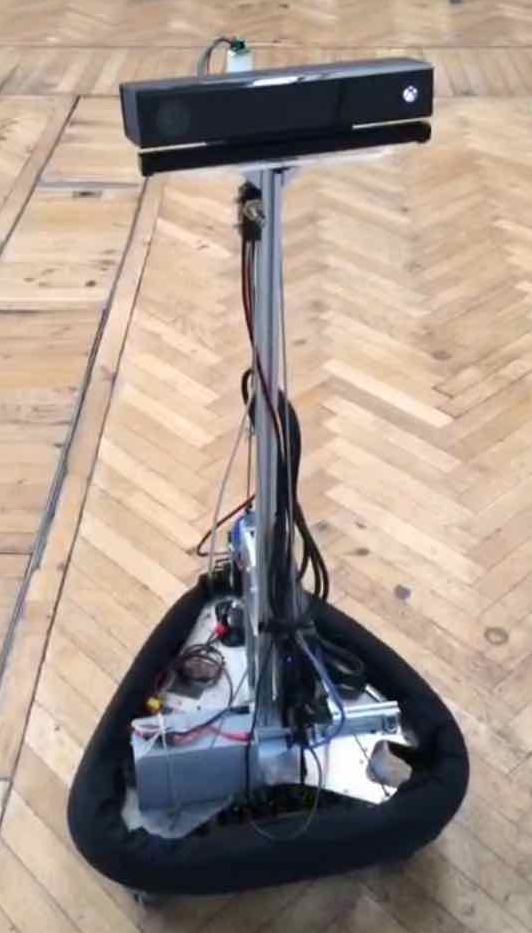
\includegraphics[height=4cm,width=2.5cm]{images/03-foundation/triskar1}}}
	  	\caption{}
	  	\label{fig:evolution_a}
      \end{subfigure}
	 ~
	  \begin{subfigure}[b]{0.22\textwidth}
		\centering
	  	\framebox{\parbox{2.5cm}{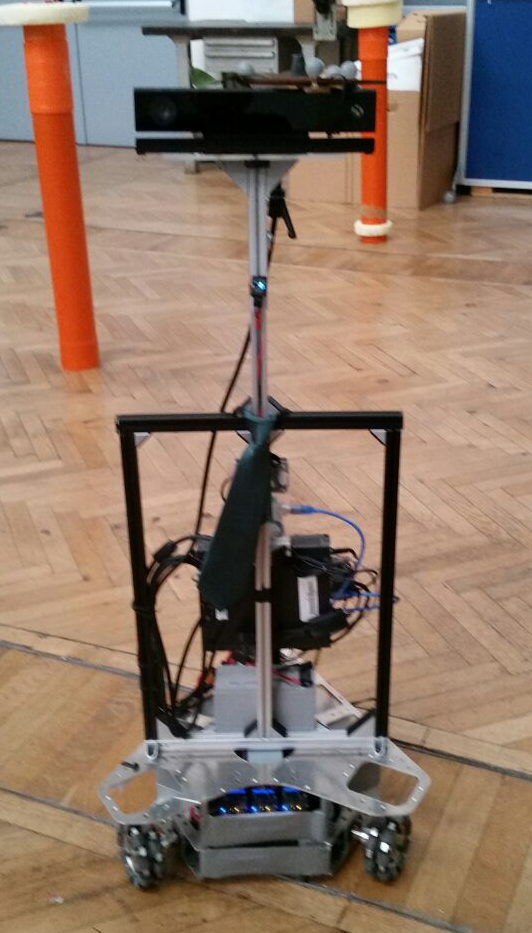
\includegraphics[height=4cm,width=2.5cm]{images/03-foundation/triskar2}}}
	  	\caption{}\label{robot}
      \end{subfigure}
      ~
      \begin{subfigure}[b]{0.22\textwidth}
      	\centering
      	\framebox{\parbox{2.5cm}{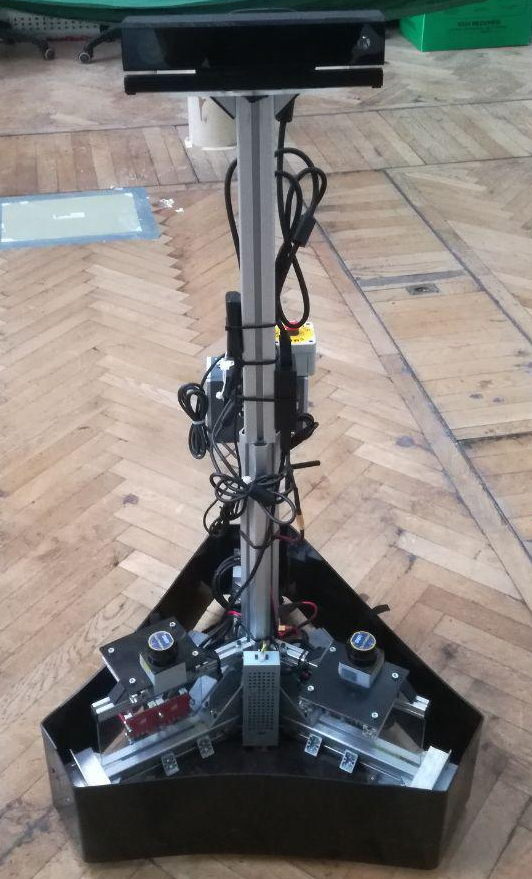
\includegraphics[height=4cm,width=2.5cm]{images/03-foundation/triskar3}}}
      	\caption{}
      \end{subfigure}
      ~
      \begin{subfigure}[b]{0.22\textwidth}
	      \centering
	      \framebox{\parbox{2.5cm}{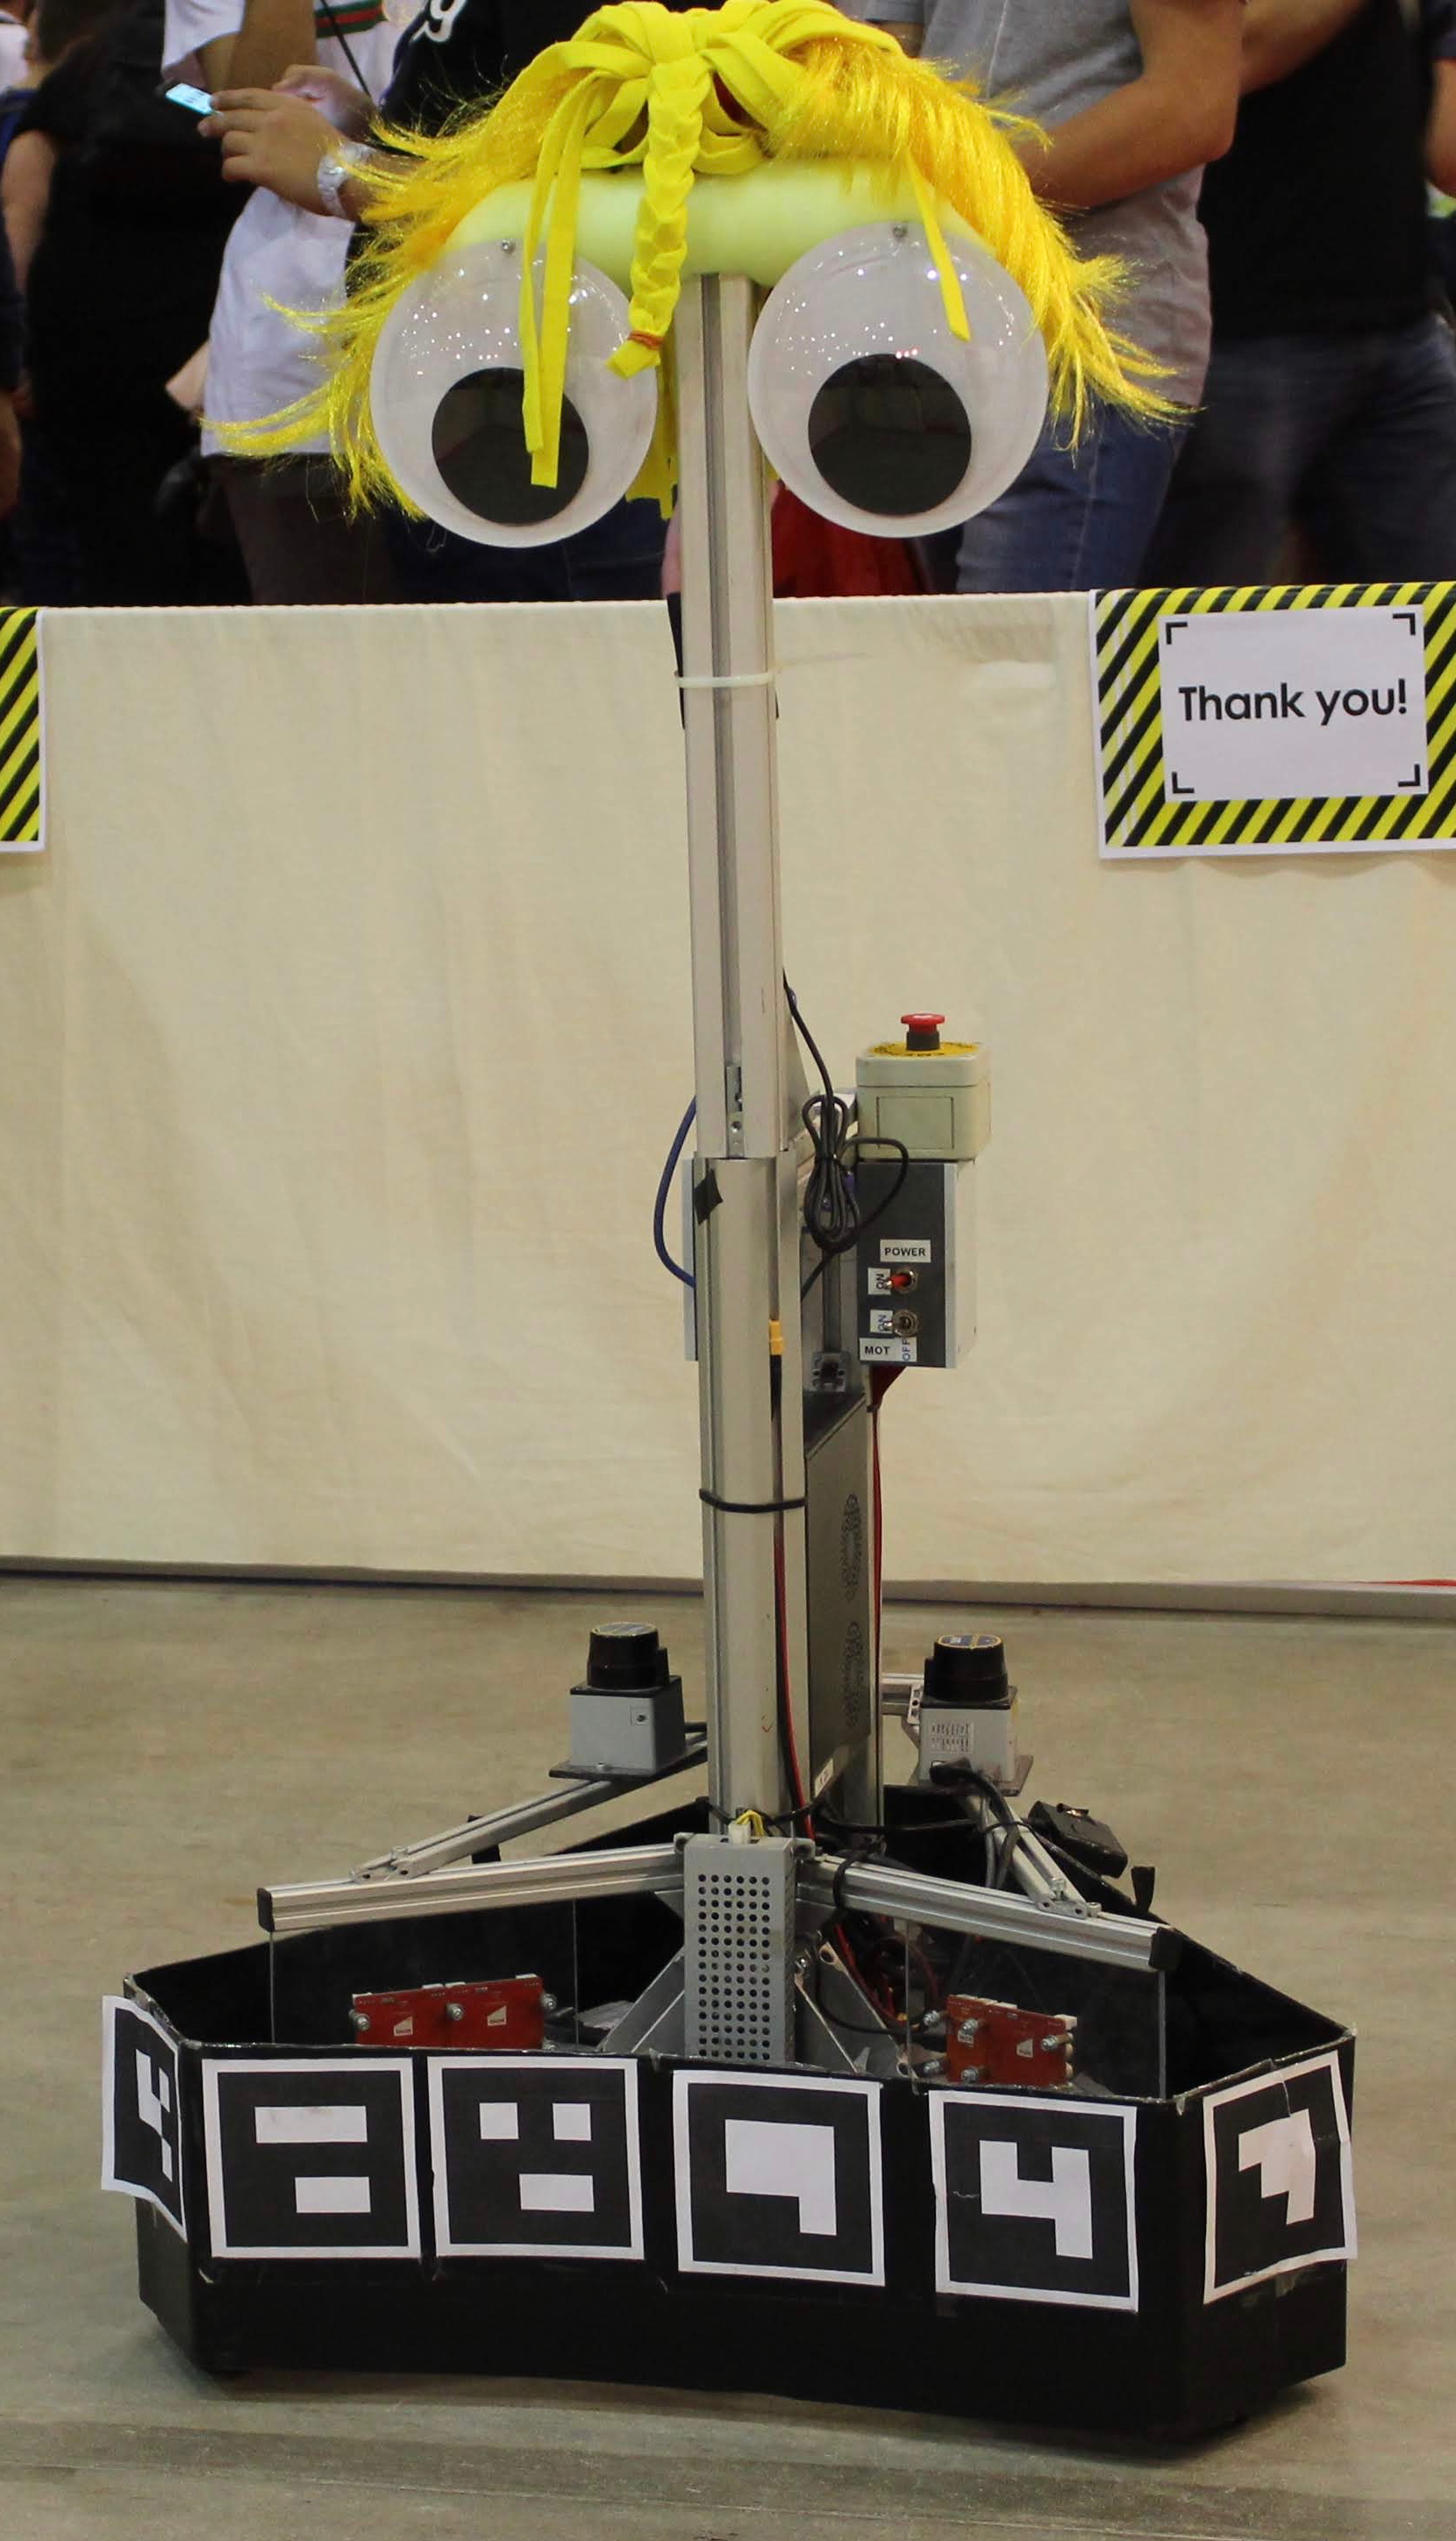
\includegraphics[height=4cm,width=2.5cm]{images/03-foundation/base4.png}}}
	      \caption{}
      \end{subfigure}
      \caption{Prototype evolution. a) First version having the Microsoft Kinect\textsuperscript{\textregistered} camera sensor support secured by steel cables in order to reduce vibration due to motion. b) Second version had improved stability by replacing the steel cables by rigid modular aluminum profiles. c) Third version had a completely redefined base including new electronics, thicker aluminum chassi, redesigned power distribution system and 2D lasers. This version also had a larger base compared to previous prototypes; d) Current version during demonstration at the Maker Faire 2018 in Rome (the European edition) from October 12th to 14th of 2018. A better placement of lasers had made the use of Kinect\textsuperscript{\textregistered} unnecessary since it allowed for full 360\textsuperscript{$\circ$} laser sensing coverage.}
      \label{fig:evolution}
\end{figure}

\subsection{Sensing}
\subsubsection{Microsoft Kinect\textsuperscript{\textregistered}\label{sec:kinectsec}}
In some phases of our development we have used the Microsoft Kinect\textsuperscript{\textregistered} sensor. It is a 3-D camera: in addition to providing an RGB image with its 1080p color camera, it also provides a depth map,  meaning that for every pixel of the depth image provided by the sensor, Kinect\textsuperscript{\textregistered} provides the distance from the sensor (see appendix~\ref{app:hard_appendix} for sensor specifications). This makes the it suitable for a variety of computer vision problems like background removal, blob detection, and people tracking.

\subsubsection{Laser scanners}\label{sec:lasers_hokuyo}
We have equipped our robot with two Hokuyo laser scanners model URG-04LX\footnote{\url{https://www.hokuyo-aut.jp/search/single.php?serial=165} accessed on \today.}. The sensors perceive the range of obstacles on a plan with a field of view of 240$^\circ$ and a resolution of 0.36$^\circ$, the maximum detectable distance is 5.6 m and they can be connected to the computer by means of a USB interface, being operated with a nominal voltage of 5V.

The Hokuyo URG-04LX consists of a compact stacked structure with a spindle motor and the actual scanner on top of it. The motor rotates a small transmission mirror that deflects the vertical laser beam coming from the top of the sensor into horizontal direction. This allows the laser beam to scan a planar area around the sensor with an opening angle of 240$^\circ$. A second mirror below, the reception mirror, deviates the horizontal laser beam captured by a lens into vertical direction again.

% \begin{figure}[H]
% 	\centering
% 	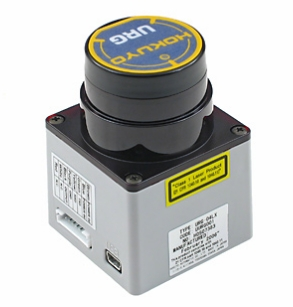
\includegraphics[width=5cm]{images/03-foundation/hokuyo}
% 	\caption{ An Hokuyo URG-04LX laser scanner.}
% 	\label{fig:hokuyo} 
% \end{figure}

A full scan is performed every 100 ms. We mounted a laser scanner on each side of the lower chassis allowing for a 360$^\circ$ coverage around the robot at a height of 30 cm from the floor.

\subsection{Structure \& Materials}
\subsubsection{Chassis}
The chassis of our robot was made entirely from modular aluminum profiles put together as to define the shape in figure~\ref{fig:aluminum_structure} (3rd prototype). The arrangement of the wheels, as to allow for the holonomic behavior, also allowed us to place batteries conveniently~(see figure~\ref{fig:batteries}) as well as the onboard computer and electronics~(see figure~\ref{fig:computer}). The careful placement of heavyweight elements, such as the lead-acid batteries, turned out to be important in our design since it impacted manoeuvrability. For instance, during test it occurred that, due to inertia, the robot would become vertically unstable when making quick turns or rapidly reacting to the human player's presence. 

The constraint of having the Microsoft Kinect\textsuperscript{\textregistered} sitting on top of a aluminum profile, as to allow maximum visibility from the sensor, moved the center of mass upwards making vertical balance worse. The void created between the wheels, in prototype versions three and four, elegantly provided a way to balance weights and make the robot's center of mass close enough to its base center. Figure~\ref{fig:evolution_a} documents the inefficient weight distribution in the first prototype. In the figure its possible to see the placement of one of the lead-acid batteries in the right side of the base, thus, making the weight distribution asymmetric.

Due to forces acting upon the robot during motion we have used software solutions for velocity smoothing that would increasingly bound speed when accelerating and decelerating. This, together with a proper weight distribution, rendered the robot's motion smooth, improving control, at the benefit of reducing the chances of mechanical breakdown caused by material stress.

\begin{figure}[ht]
    \centering
    \begin{subfigure}[b]{0.22\textwidth}
      	\centering
        \framebox{\parbox{2.5cm}{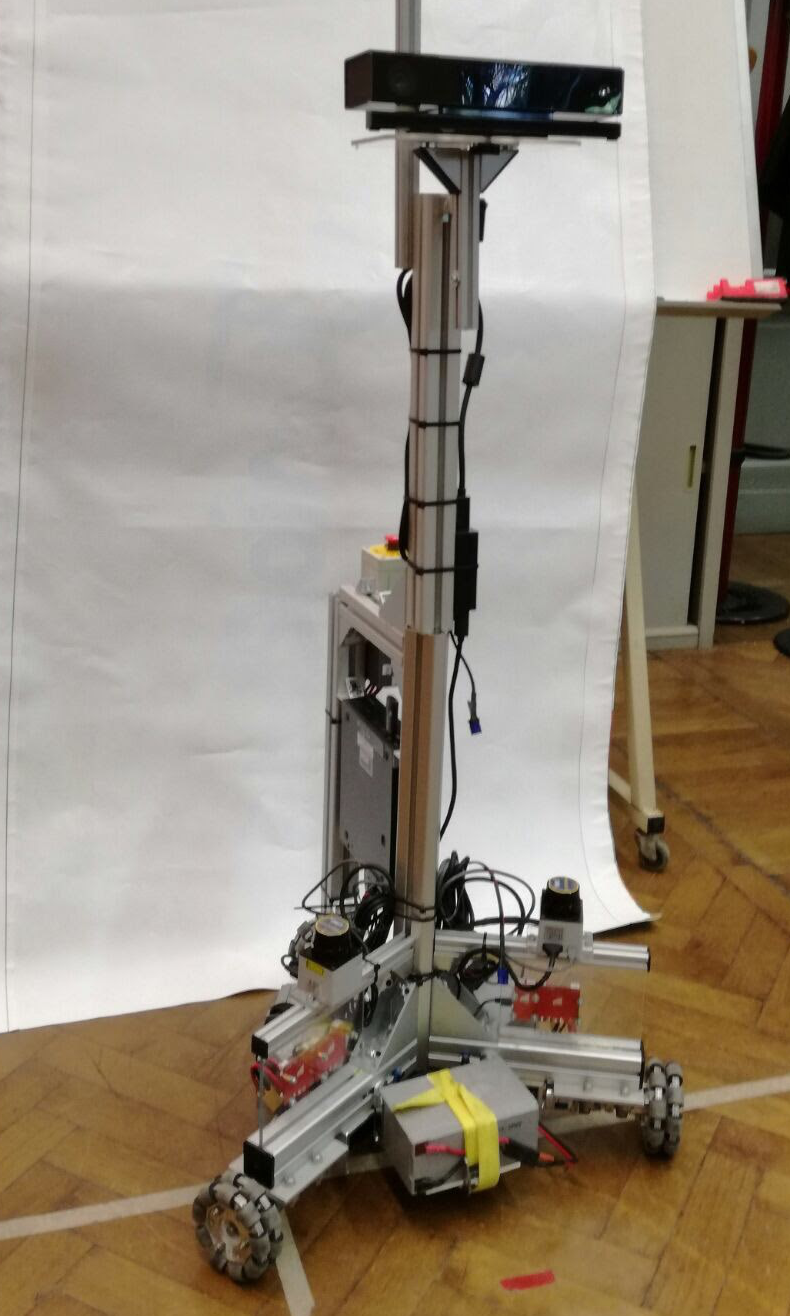
\includegraphics[height=4cm,width=2.5cm]{images/03-foundation/structure}}}
        \caption{}
        \label{fig:aluminum_structure}
    \end{subfigure}
    ~
    \begin{subfigure}[b]{0.22\textwidth}
      	\centering
        \framebox{\parbox{2.5cm}{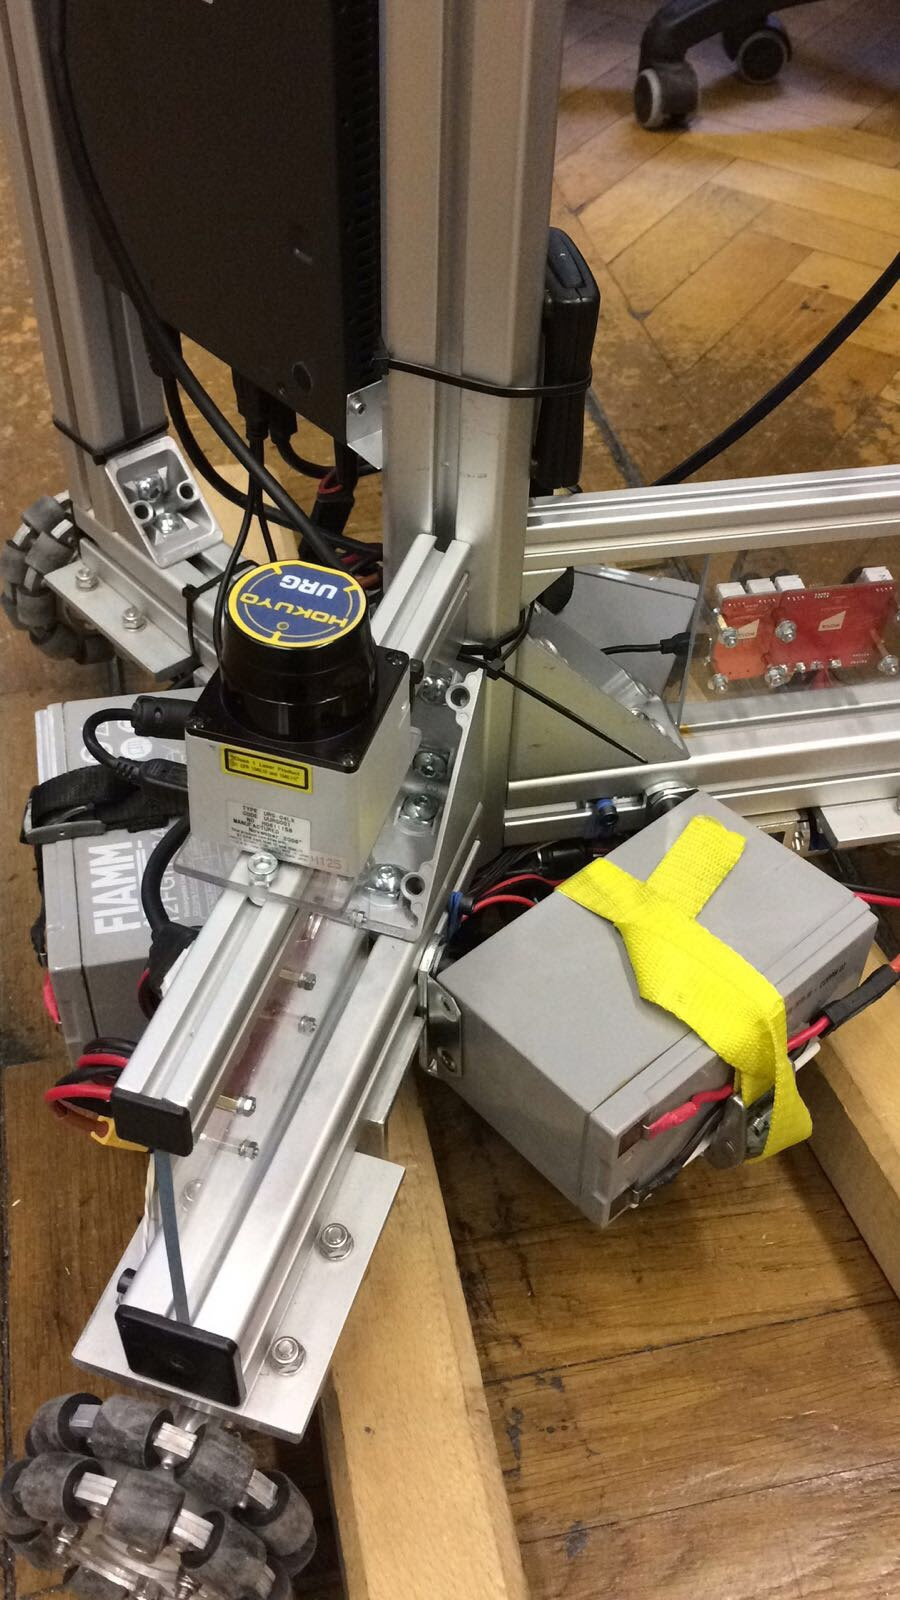
\includegraphics[height=4cm,width=2.5cm]{images/03-foundation/structureII}}}
        \caption{}
        \label{fig:batteries}
    \end{subfigure}
    ~
    \begin{subfigure}[b]{0.22\textwidth}
      	\centering
        \framebox{\parbox{2.5cm}{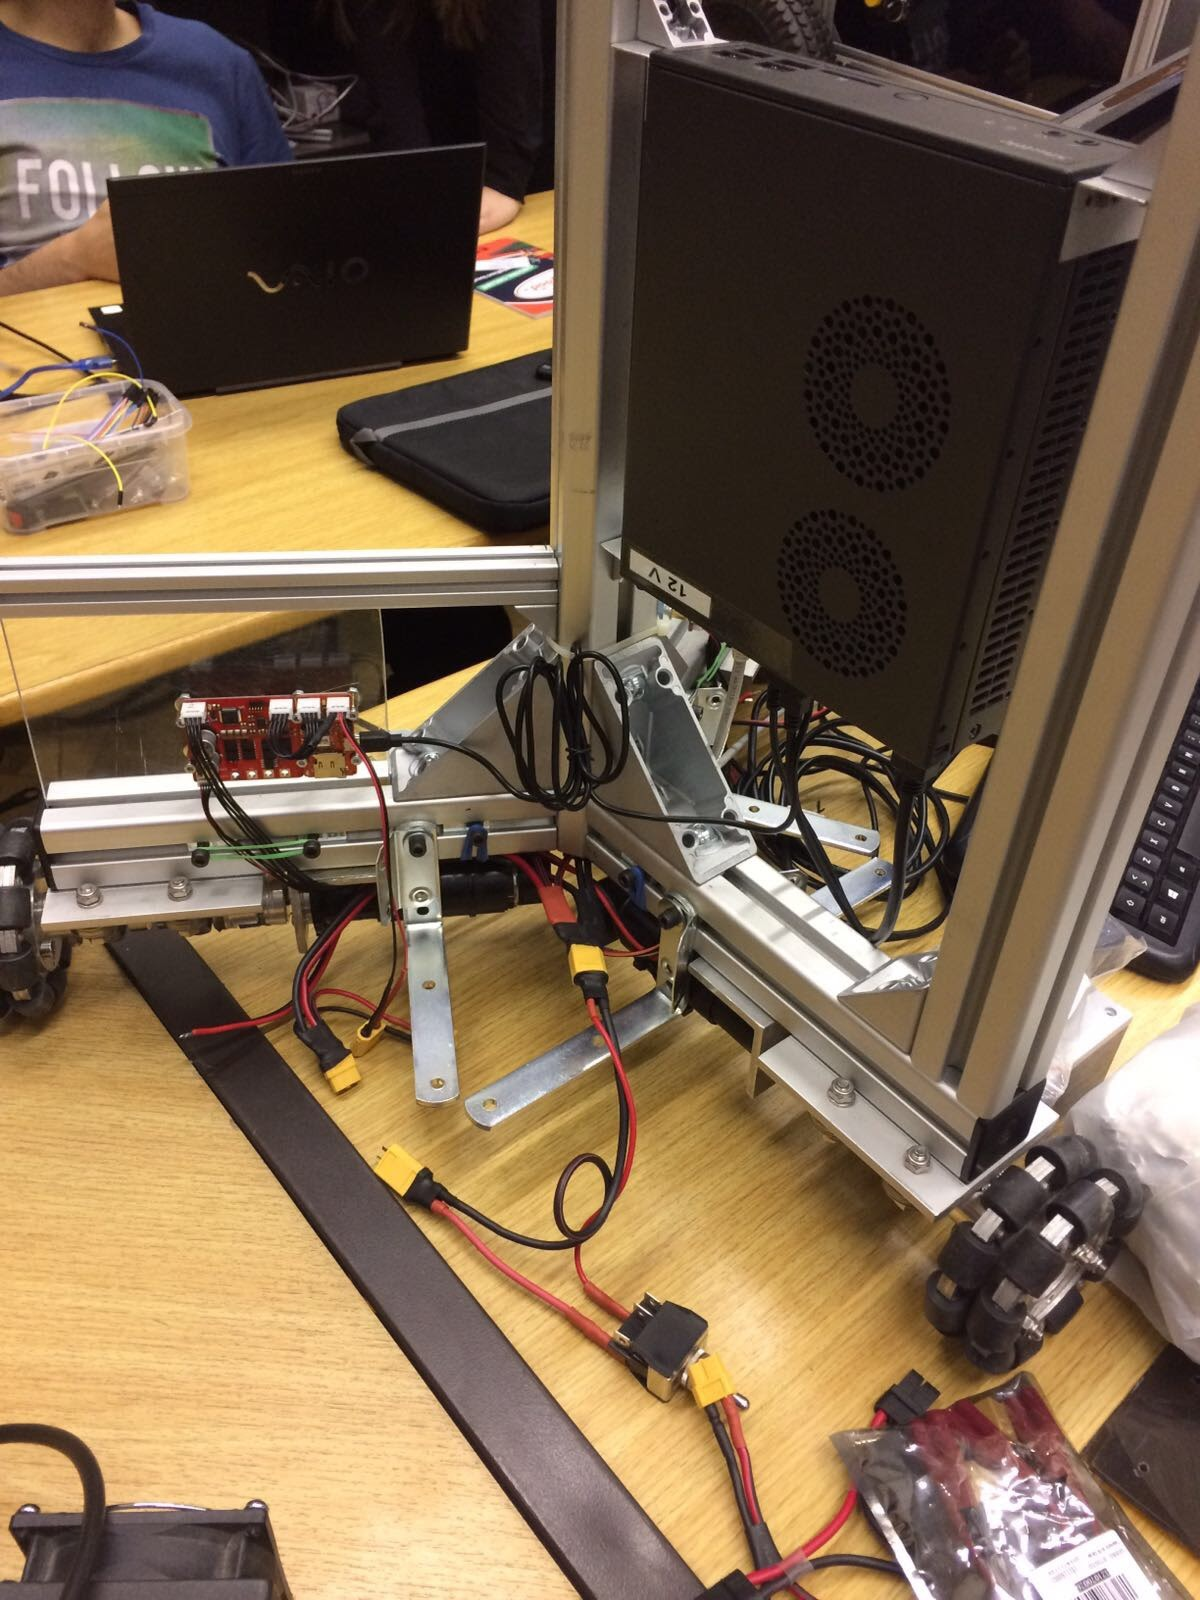
\includegraphics[height=4cm,width=2.5cm]{images/03-foundation/structureIII}}}
        \caption{}
        \label{fig:computer}
    \end{subfigure}
    \caption{Structural details of our robot. The chassis is made of modular aluminum profiles from which rapid and easy prototyping is possible while retaining a good level of robustness. a) The full scale view of the robot (3rd version). b) a close-up view of one of the 2-D lasers and batteries (gray boxes). c) a close-up view of the vertical placement of computer (black box) and control board (red board).}
    \label{fig:structure_details}
\end{figure}

\subsection{Kinematics}
As said before, our robot had holonomic kinematics. Holonomy being referred to existing restrictions applied among translational axes. If a robot is holonomic with respect to $N$ dimensions, it's then capable of moving in any direction in any of the $N$ physical dimensions available to it. Our robot  matches the kinematics of a human player well, since it is possible to refer to humans as holonomic within two-dimensional space. Mathematical details regarding a 3-wheel omnidirectional robot is given in appendix~\ref{app:hard_appendix}.

\subsection{Power Supply}
Our robotic platform operated at a nominal voltage of 24V with two lead-acid 12V batteries connected in series. A DC-DC board was used to regulate the input voltage down to 12V, which was the nominal voltage for the onboard computer and Kinect\textsuperscript{\textregistered} device -- both being powered independently through the DC-DC. The motors, were powered directly from the 24V via a separate circuit with an independent turn on/off switch and emergence button. Having separate circuits with independent switches was necessary in order to allow for turning off the motors (in case of an emergence) independently of the electronics (computer, sensors and control board). The two lasers were powered via USB connection to the PC. The power  configuration allowed for a total time of 40 minutes before demanding battery replacement. Details regarding the batteries and electrical circuits are described in appendix~\ref{app:hard_appendix}.

\subsection{Computing \& Electronics}
\subsubsection{Onboard computer}\label{onboard pc}
For computing a Shuttle XPC Slim DH270 was used. The device has a $190 \times 165 \times 43$~mm steel case, and weights $1.3$~kg.  The armature presents two holes for Kensington Locks and numerous threaded holes (M3) at both sides allowing for an easy placement. The operating system used was~\textit{Ubuntu 16.04.3 LTS (64bit)}. The computer had an Intel Core i7 and a RAM DDR4 memory of 16 GB .

\subsubsection{Control boards}\label{novacore}
The low-level motors actuation and their interface between the ROS system have been realized with the Nova Core modules based on STM32-chip~\footnote{\url{http://www.novalabs.io/} accessed on \today.}, which implement ready to use components to fulfill robot prototyping requirements with plug \& play approach.  
The provided modules allow to control different type of motors that can be modeled as a second order system, where the input is the voltage applied to the motor armature and output variable is the motor angular speed. Futher details about the deployed boards are presented in figure~\ref{fig:boards}.

\begin{figure}[ht]
  \centering
  \begin{subfigure}[b]{0.3\textwidth}
  \centering
      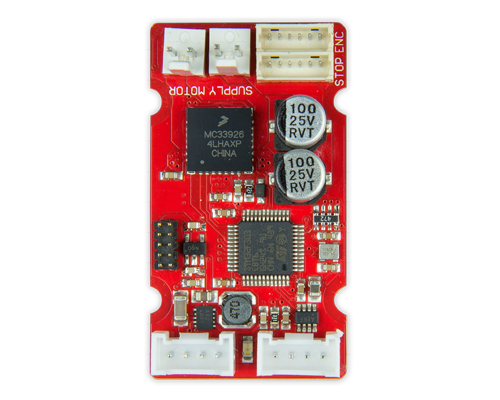
\includegraphics[width=3cm,height=2.5cm]{images/03-foundation/udc}
	\caption{}
  \end{subfigure}
  \begin{subfigure}[b]{0.3\textwidth}
  \centering
      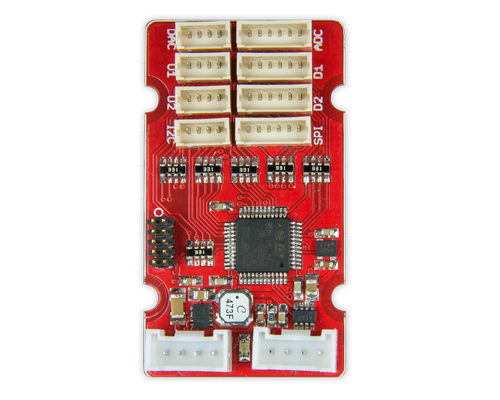
\includegraphics[width=3cm,height=2.5cm]{images/03-foundation/io}
	\caption{}
  \end{subfigure}
  \begin{subfigure}[b]{0.3\textwidth}
  \centering
      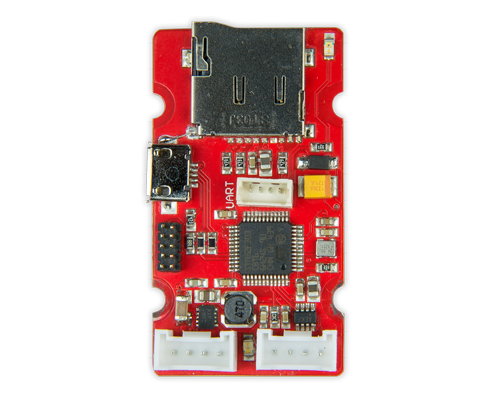
\includegraphics[width=3cm,height=2.5cm]{images/03-foundation/usb}
	\caption{}
	\label{fig:usb_board}
  \end{subfigure}
  \caption{a) UDC board (1 per each motor) capable of driving motors up to 70 W, with torque, speed, and position closed loop control. General attributes: 5-28V supply; 3A max (5A peak); current sense; encoder input; limit switch input; 25 x 45 mm in size. b) IO board (1 per each motor): Integrate existing hardware into the real-time Nova Core bus with analog and digital signals. General attributes: 8 digital GPIO;  4 analog inputs; 2 analog outputs; 2 UART; 1 I2C; 1 SPI; 25 x 45 mm in size. c) USB board (used for data collection) Interface the real-time Nova Core bus with a computer and logs data to microSD memory. General attributes: USB connector;  UART connector; microSD card slot; rosserial support; 25 x 45 mm in size.}
  \label{fig:boards}
\end{figure}
%ANDY all the technical details and names of devices could go in an appendix, while I'll leave here a functional description of robot and sensors, giving the characteristics that are functionally relevant, e.g., speed, omnidirectionality, range of sensors, their data rate, ...

\subsection{Navigation}
\subsubsection{\glsdesc{slam}}\label{gmapping}
To create a map of the environment, our system used \textit{gmapping}\footnote{http://wiki.ros.org/gmapping accessed on \today}, a ROS package used for~\gls{slam} that estimates the map of the environment and the trajectory of the robot using a technique known as~\gls{rbpf}~\citep{grisettiyz_improving_2005} and the provided odometry and laser measurements. The procedure in\textit{gmapping} can be decomposed in two phases: \begin{inparaenum}[\itshape a\upshape)]\item update the robot's state using all available positioning related data. In our case, odometry and laser measurements was used; \item update the map of the environment using~\gls{rbpf}.\end{inparaenum}

The obtained map is an occupancy grid and it is represented as an image showing the blueprint of the environment. Once created, the integrated localization in ROS will be able to generate reference frame transforms from the map-frame to the robot odometry frame, correcting for estimated position in the environment. In Figure~\ref{fig:playground_map} an example of map is shown, with tower positions being clearly visible.

Considering only the playground (area of the rectangle delimited by four towers), however, introduce several problems to the localization algorithm. For instance, when the playground is put in a rectangular room with only the towers as ``furniture'' the symmetry of the environment does not possess enough descriptive features to infer the position unequivocally and localization is worsened. For this reason it was needed to include enough descriptive features around the playground borders to enhance the robot localization during the game. The map in figure~\ref{fig:playground_map} is a good example of a map with good features since the walls around the playground are ``jagged enough'' to distinguish the walls among themselves. 

\begin{figure}[h]
	\centering
	\framebox{\parbox{5cm}{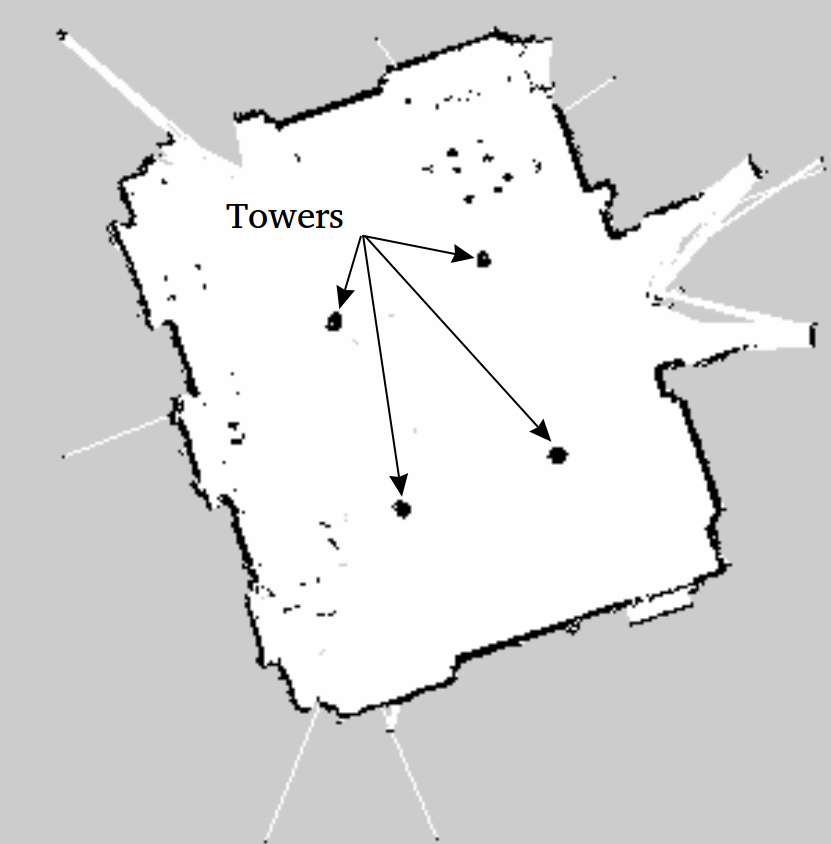
\includegraphics[width=5cm]{images/03-foundation/playgroundmap}}}
	\caption{Map of the room with playground obtained with gmapping algorithm.} 
	\label{fig:playground_map}
\end{figure}

In particular, aiming at standardizing the map across different environments, reduce the number of times it had to be remade and filter out noise, we have decided to enclose the playground by ``walls'' made from fabric and supported by lightweight aluminum profiles joined together. A custom entrance made in one of the sides made up for the element breaking the symmetry and allowing for effective localization. This arrangement could easily be reused without having to remake the map. Enclosing the area was particular useful when collecting data since very often~\gls{pirg}s tend to gather a number of people around the playground which can compromise the environmental perception by the robot. Furthermore, it allowed us to reduce the complexity of tracking the player, as it is going to be explained later. 

\subsection{Tower navigation}
In this section we describe the algorithm that enables the robot to navigate from its current position to a target tower and its implementation. For this purpose, a point-to-point trajectory following approach has been considered. The proposed strategy is composed of three main part: sensor data analysis, obstacle detection and goal seeking. In general, with our navigation we wanted to provide a certain level of challenge to the human player while also trying to minimize behaviors that could lead to odometry errors and loss of localization in the map. The selection of the target tower takes into account the proximity relationship between the current position of the robot and that of the human player. The particular algorithm for that is going to be presented later as well as the mechanism for player tracking.

For the navigation, we focused in particular on avoiding wheel slippage during the initial acceleration phase. Generally, the selection of a target tower by the robot is performed such that the direct path leading to it is as free as possible considering the current player's position. 

During navigation, in case the human player is detected below a certain safety distance from the moving robot, the algorithm switches to the obstacle avoidance procedure described in section~\ref{sec:obt_avoidance}. As inputs to the navigation algorithm, we consider: the robot's estimated $x$ and $y$ position ($\hat{x}_R$, $\hat{y}_R$); target tower xy-coordinate ($x_G$, $y_G$) and a flag variable that assumes the value false if the robot is approaching an obstacle (\textsc{is\_safe}). The raw outputs are: the unsmoothed xy-linear velocity in the world frame ($\dot{\bar{x}}_R$, $\dot{\bar{y}}_R$) and a a flag variable that is true if the robot is close to a targeted tower (\textsc{near\_goal}). The procedure for generating velocity commands to the platform is detailed in algorithm~\ref{alg:pointopoint}. At each control loop call the algorithm publishes a new velocity command.

\begin{algorithm}[ht]
	\# define initial e final points when the robot receives the id of the targeted tower \;
	$x_d$ = ($\hat{x}_R$, $x_G$)\;
	$y_d$ = ($\hat{y}_R$, $y_G$)\;
	\# define the robot deviation from the required trajectory\;
	$\Delta x = x_d[1] - x_d[0]$\;
	$\Delta y = y_d[1] - y_d[0]$\;
	\# generates the direction of the motion based on the euclidian distance from goal\;
	goal\_distance$ = \sqrt{({\Delta x}^2 + {\Delta y}^2)}$\;
	$\alpha = $\textbf{atan2}$(\Delta x, \Delta y)$\;
	\# check if the robot is near its goal (this will trigger the obstacle avoidance behavior)\;
	\If{(goal\_distance < NEAR\_GOAL\_Treeshold)}{
		near\_goal = true\;
	}
	\# SAFETY CHECK: the controller will generate velocity commands only if the safety condition is satisfied. if safety condition is satisfied then: enable == 1 (player not too close to the robot);\;
	\If{(is\_safe = true)}{
		$\dot{\bar{x}}_R=V_\text{max}\cdot\cos(\alpha)$\;
		$\dot{\bar{y}}_R=V_\text{max}\cdot\sin(\alpha)$\;
	}
	
	\Return $\dot{\bar{x}}_R$, $\dot{\bar{y}}_R$, is\_safe 
	\caption{Point-to-Point navigation algorithm.}
	\label{alg:pointopoint}
\end{algorithm}

Prior to the execution by the low-level sub-systems that control the motors, the velocity vector $<\dot{\bar{x}}_R,\dot{\bar{y}}_R>$ output by algorithm~\ref{alg:pointopoint} need further processing. Specially, it needs to be transformed from the world reference frame (the frame in which towers are located in) to the robot reference frame (see transformation details in appendix~\ref{app:hard_appendix}).

Another aspect that had to be addressed was that of guarantying the decoupling between robot rotations and translations. The control of the robot orientation had to be completely independent from the xy-translation, since the robot in our scenario had to be able to track the movement of the human player while navigating towards the target towers. Mathematical detail of this process is once again available in appendix~\ref{app:hard_appendix}. With this approach, the transformed velocity set-points $\dot{\bar{x}}_R^m$ and $\dot{\bar{y}}_R^m$, dynamically change during the game and often the variation has a step-function shaped form that causes the low level actuation to react violently to make the robot reach the desired velocity at once -- especially when starting from the initial position with 0-velocity (see figures~\ref{vel14} and~\ref{wheel14}). This will result in the robot wheels undergoing in slippage due to the too sharp acceleration required to reach the velocity set-point. This is an undesired effect that is source of non-systematic odometry errors that may lead to instability and loss of localization. 

A number of tests have been performed to quantify the effect of wheel slippage during the initial robot acceleration phase. In these tests the robot linearly translates along $x$ and $y$ axis and receives the initial velocity set-point at $1m/s$ or $1.4m/s$. In figures~\ref{opti14},~\ref{amcl14},~\ref{poserror14},~\ref{opti14y},~\ref{amcl14y}, and~\ref{poserror14y} we can see the localization error introduced during such test.

To avoid this effect, a velocity smoother has been used in order to obtain a smooth velocity set-point control signal to be sent to the robot low-level actuation, towards avoiding wheels slippage during the acceleration phase. The inputs of the velocity smoother are the unsmoothed velocity set-points [$\dot{\bar{x}}_R^m$, $\dot{\bar{y}}_R^m$], some of the internal parameters such as maximum allowed velocity and maximum allowed acceleration can be changed online to modify the final response of the robot. The output are the final xy-velocity control signals [$\dot{x}_R^m$, $\dot{y}_R^m$] in robot reference frame that will be sent to the low level actuation.

The velocity smoother runs together with algorithm~\ref{alg:pointopoint}, receiving the output of this later as input. It basically pre-filters any incoming command input based on some acceleration constraints. Smoothing velocities are not just important for the reduction of localization errors, but is also an important factor in the reduction of material stress on the wheels, which can lead to mechanical breakdowns. In fact, during our research we have had a couple of mechanical breakdown due exactly to excessive acceleration. Such issues make up for important example of typical hardware concerns and issues on must deal with in the design of mobile agents for~\gls{pirg}.

\subsubsection{\glsdesc{oa}}\label{sec:obt_avoidance}
For in-game obstacle avoidance, a fuzzy-logic based reactive control has been designed to respond appropriately to sensory input. This was used principally because the human player could move completely unconstrained through the playground,~\ie proximity between human and robot could be sensed from any direction and in any moment during the game. Having fuzzy-logic rules for the decision making provided much soft navigation and stable control since a fuzzy approach can handle well the uncertainty when the sensed obstacle is at the boundary of sensing areas.

As first step, considering the laser sensing capabilities of our robot (see section~\ref{sec:lasers_hokuyo}), we have divided the rays cast from the laser into different discrete sensing areas around the platform. The information  contained in each laser scan message received from the ROS Hokuyo node (published in the topic \textit{/scan}) is composed of 1000 rays, each one of which carrying information about the distance and bearing angle of the sensed object w.r.t the sensor origin. The laser scan data was divided by indexes as follows:

\begin{itemize}
	\item \textbf{Rear Right:} indexes from 1 to 150;
	\item \textbf{Right:} indexes from 151 to 310;
	\item \textbf{Front Right:} indexes from 311 to 500;
	\item \textbf{Front Left:} indexes from 501 to 690;
	\item \textbf{Left:} indexes from 691 to 851;
	\item \textbf{Rear Left:} indexes from 850 to 1000.
\end{itemize}

For each area, the minimum distance to objects are calculated and a flag variable monitors whether an obstacle is within a given threshold distance (in our case $0.75$ meters). When this condition is verified, the fuzzy obstacle avoider takes the control from the trajectory navigation in order to handle the obstacle at hand. When the robot is close within a specified distance threshold from a target tower the obstacle avoider is disabled, thus, enabling it to tear down the towers instead of considering them as obstacles. In general, the output of the avoider is the tuple $(V_{x\_\text{avoider}}, V_{y\_ \text{avoider}})$ controlling the xy-translations.

when calculating the membership of an obstacle w.r.t. a sensory region, if the minimum distance of a sensing sector has index belonging to the fuzzy areas the ``crisp'' output values after defuzzyfication will be a mixture of the results of the rules associated to the two contiguous sectors. The membership functions shown in figure~\ref{indexesmmf} illustrates the idea. On the x-axis are reported the index values in a range from 1 to 1000, each one of it representing one of the 1000 laser's ray distance measurement that the system receives from each ROS /scan message.

For capturing the minimum detected distance in each sector the membership functions shown in figure~\ref{minmmf} had been defined. The x-axis ranges from 0 to $0.75$ meters (as said, the obstacle avoidance takes control of the robot's navigation when obstacles are detected below this threshold) the three labels \textit{``Close''}, \textit{``Far''}, and \textit{``Dontcare''} were used to define the intensity of the control action during the obstacle avoidance maneuver.

\begin{figure}[H]
	\centering
	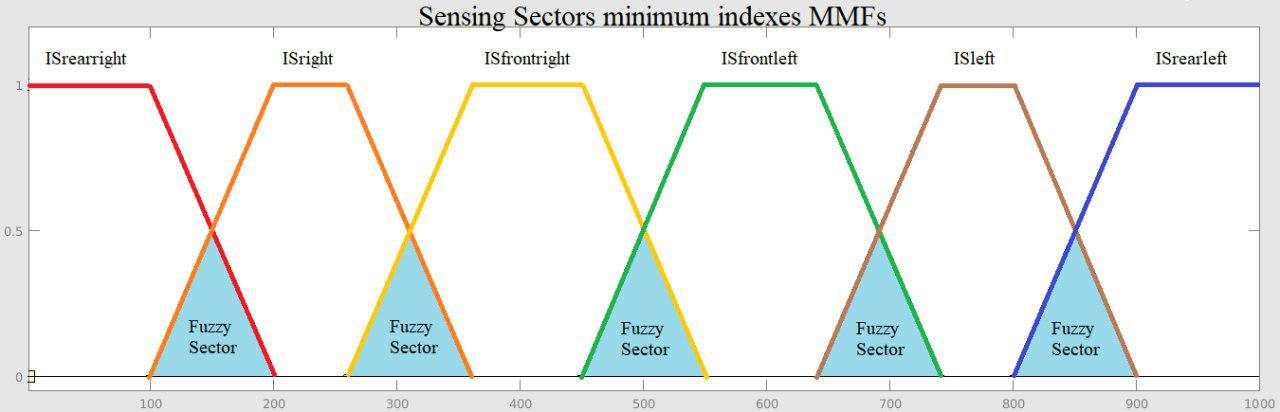
\includegraphics[width=\textwidth]{images/03-foundation/indexesmmf}
	\caption{Membership functions (MMFs) for minimum detected distance \textit{index} in each sensing sector.}
	\label{indexesmmf} 
\end{figure}
\begin{figure}[H]
	\centering
	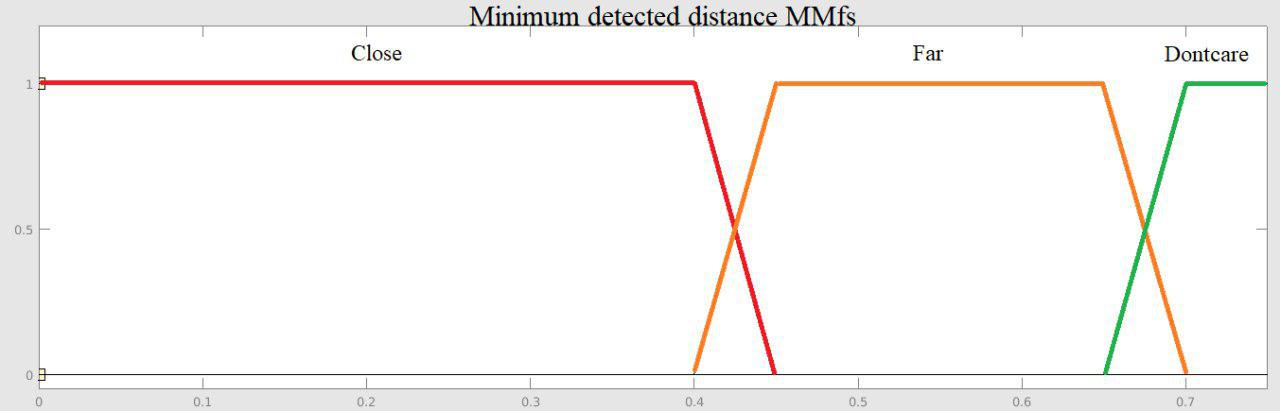
\includegraphics[width=\textwidth]{images/03-foundation/minmmf}
	\caption{Membership functions (MMFs) for minimum detected distance \textit{index} in each sensing sector.}
	\label{minmmf} 
\end{figure}

The system uses a Mamdani-type inference that requires the output membership functions to be fuzzy sets. After the aggregation process, \ie after evaluating the result of each rule, these results are combined to obtain a final result. There is a fuzzy set for each output variable that needs defuzzification.

The used defuzzification method was the ``Centroid'' method that returns the center of mass of the area under the curve, it can also be seen as a Center of Gravity and can be obtained with equation~\ref{centroid}:
\begin{equation}
U=\dfrac{\int_{\text{min}}^{\text{max}} u\cdot\mu(u) du}{\int_{\text{min}}^{\text{max}}\mu(u) du}
\label{centroid}
\end{equation}
where U is the center of gravity, $u$ is the output variable and $\mu(u)$ is the membership function after the accumulation, implemented as the maximum. Letting $\mu_A(u)$ and $\mu_B(u)$ be the membership functions for fuzzy sets A and B and for OR and AND operators are max and min, respectively.
\begin{align}
	\textbf{Accumulation method}\qquad max\lbrace\mu_A(u),\mu_B(u)\rbrace\\
	\textbf{OR (union)}\qquad max\lbrace\mu_A(u),\mu_B(u)\rbrace\\
	\textbf{AND (intersection)}\qquad min\lbrace\mu_A(u),\mu_B(u)\rbrace
\end{align}
As output membership functions, singletons have been selected. This enhances the efficiency of the defuzzification process because it greatly simplifies the computation required by the more general Mamdani method, since, instead of finding the centroid of a 2-D function by integrating across the two-dimensional function to find the centroid, the weighted average of a few data points is used as shown in equation~\ref{singletoncentroid}, where $p$ is the number of singletons.

\begin{equation}
U =	\dfrac{\sum_{i=1}^{p}\left[u_i,\mu_i\right]}{\sum_{i=1}^{p}\mu_i}
\label{singletoncentroid}
\end{equation} 

The singletons membership functions for $V_{x\_ \text{avoider}}$ and $V_{y\_ \text{avoider}}$ are reported in figure \ref{outmmf}

\begin{figure}[h]
	\centering
	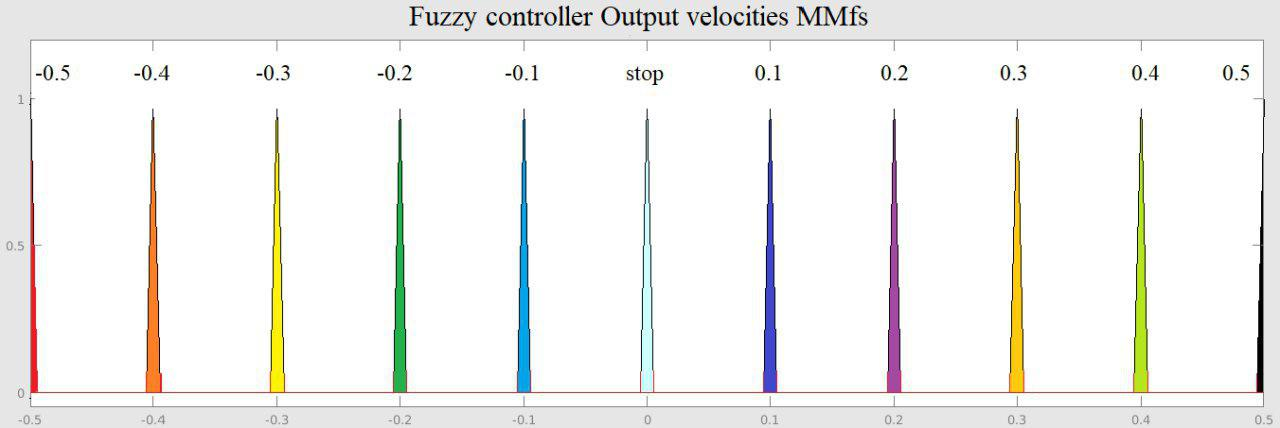
\includegraphics[width=\textwidth]{images/03-foundation/outputmmf}
	\caption{MMfs for $V_{x\_ \text{avoider}}$ and $V_{y\_ \text{avoider}}$, the output velocities along xy-axis range from -0.5 m/s to 0.5 m/s}
	\label{outmmf} 
\end{figure}

A set of fuzzy rules (reported in appendix~\ref{app:hard_appendix})	has been implemented to obtain an overall obstacle avoidance behavior that has been inspired from the artificial potential fields approach. The rules have been designed to mimic a repulsive field that will drive the robot away from obstacles when these are encountered during navigation (figure~\ref{avoid1}). In particular, when the robot reaches the condition of proximity with the human player during the game, the set of fuzzy rules will cause the robot to drift away from him until the proximity condition is no more verified ($is\_safe$ equals true. Refer to algorithm~\ref{alg:pointopoint}). At this point, the robot will go back to the normal point-to-point navigation to reach the selected target tower.

Since the ultimate goal of the robot is to physically tear down one of the four towers that are placed in the playground, the fuzzy rules also implement an attractive effect (figure\ref{avoid2}) that is exerted by the target tower when the robot comes close to it  ($near\_goal == true$, again refer to algorithm~\ref{alg:pointopoint}).

\begin{figure}[H]
	\centering
	\begin{subfigure}[b]{0.4\textwidth}
		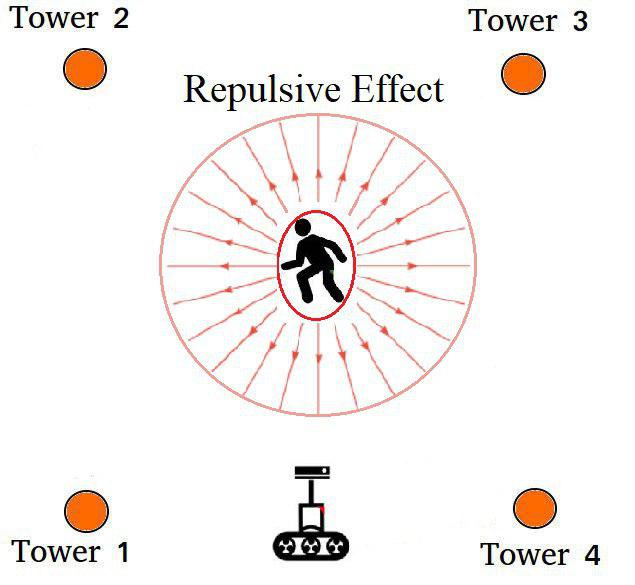
\includegraphics[width=5cm]{images/03-foundation/avoid1}
		\caption{}
		\label{avoid1} 
	\end{subfigure}
    ~
	\begin{subfigure}[b]{0.4\textwidth}
		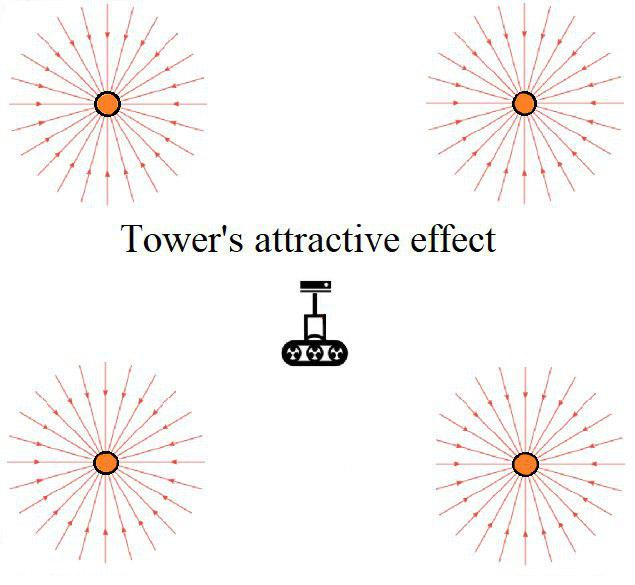
\includegraphics[width=5cm]{images/03-foundation/avoid2}
		\caption{}
		\label{avoid2}
	\end{subfigure}
	\caption{a) Representation of the repulsive effect implemented by the fuzzy rules. b) Representation of the attractive effect implemented by the fuzzy rules. }
	\label{rulesbehavior}
\end{figure}

\subsection{Player perception \& tracking}
For opening the device, we have used libfreenect2\footnote{~\url{https://github.com/OpenKinect/libfreenect2} accessed on \today.}, a library for managing the Kinect\textsuperscript{\textregistered} device on Linux. We have then created a custom tracking node capable of estimating the player's position in two phases: First, color blob detection. Second, segmentation on the depth frame using \textit{region growing} algorithm for the purpose of detecting the player's body. Two features can be detected from this procedure: distance (relative to the robot) and contraction index. The first is calculated from the mean value of the depth pixels around the center of the blob. The latter is computed based on the subtraction of the occupied area with respect to the dimension of the bounding box that encompasses the segmented silhouette (see Figure~\ref{fig:segmenta}). This feature had been considered as a cue about the fact that the player was opening arms, so, possibly, actively participate to the game.

\begin{figure}[h]
  \centering 
  \begin{subfigure}[b]{0.3\textwidth}
		\centering
		\framebox{\parbox{3cm}{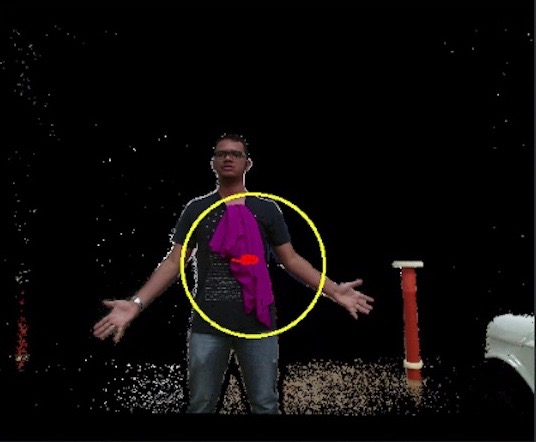
\includegraphics[width=3cm, height=3cm]{images/03-foundation/point_cloud}}}
		\caption{}
  \end{subfigure}
  ~
  \begin{subfigure}[b]{0.3\textwidth}
		\centering
		\framebox{\parbox{3cm}{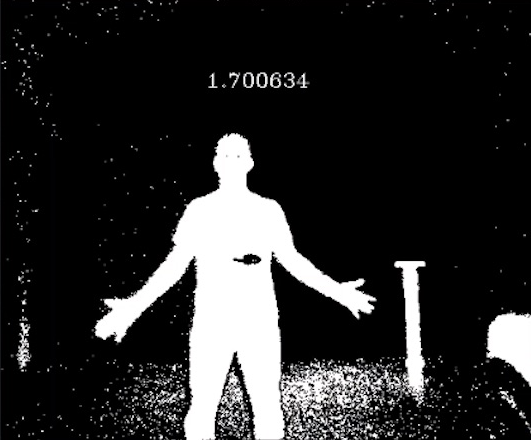
\includegraphics[width=3cm, height=3cm]{images/03-foundation/depth}}}
		\caption{}
  \end{subfigure}
  ~
  \begin{subfigure}[b]{0.3\textwidth}
		\centering
		\framebox{\parbox{3cm}{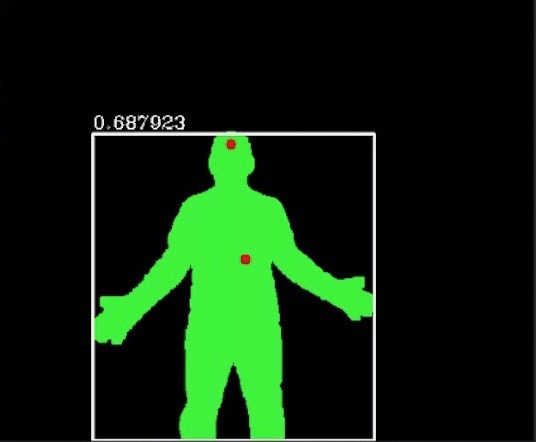
\includegraphics[width=3cm, height=3cm]{images/03-foundation/segmentation}}}
		\caption{}
  \end{subfigure}
  \caption{Example of frames processed by our algorithm. a) Point cloud showing the center of the detected (light-purple) color blob. b) Depth frame. The number showed above the user correspond to his estimated distance relative to the robot (in meters). c) Segmentation results. The number above is the contraction index defined in the interval [0,1] and can be used as a measure of body contraction.}\label{fig:segmenta}
   \label{segmentacao}
\end{figure}
\chapter{Playing for competitive advantage}\label{ch:playing_for_advantage}

As exposed in section~\ref{sec:dimensions}, one important dimension in the design of~\glspl{pirg} is that of playing for competitive advantage. This is not a special dimension of design present only in this type of application, but an intrinsic one necessary in all rational adversarial playing agents, both physical and virtual. Before designing the part of the system supporting  entertainment, which is the focus of our research and experiments, one must design the basic mechanism to enable the robot to take actions to win the game,~\ie take actions that satisfy the rules imposed by the game itself in the best possible way and act to profit of them -- which means being rational w.r.t the actions available in each game state. 

We recall that a low level of rationality shown by~\gls{pirg} agents is deemed to have negative impact on acceptability and fun~\citep{martinoia_physically_2013}. Playing for the purpose of human player entertainment in this scenario is not a trivial and can potentially have conflicting goals w.r.t. the objective of playing for competitive advantage. In general, one must trade-off the influence of the action planning in the general robot behavior so as to maintain a reasonable level of rationality while engaging players. In practice, this implies making a change in the utility function to incorporate aspects that make the game more enjoyable. Here, for our purposes, we decided to keep the two dimensions of play separate as depicted in figure~\ref{graph:PIRG_design_structure}. This allows for the modulation in playing for engagement while maintaining a working baseline for the competitive capability. Additionally, it makes up for easy code maintenance by separating the respective dimension requirements. In this chapter we describe how the robot plays for competitive advantage in our~\gls{pirg} scenario.

\section{Competitive advantage in RoboTower 2.0}\label{sec:competitive_adv_robotower2}

For our robot, action selection had at least three main concerns, namely: planning, timing and safety issues (see figure~\ref{graph:COMPETITIVE_structure}). The adopted planning algorithm was fast enough to provide the current best next tower to attack based on the current position of the robot and player with high frequency.

Although fast, for our game we had to constrain the system to take decision at a maximum frequency of 1Hz so as to help the player process better the game dynamics and have enough time to plan ahead and/or to rest. It became clear in the test phase that leaving the robot take decisions at a higher frequency would make the game very difficulty. Despite being a concern more related to the goal of playing for entertainment, the frequency constraint was considered necessary at this phase in order to make the game playable. 

\begin{figure}[H]
    \centering
    \begin{tikzpicture}[ every annotation/.style = {draw,
                         fill = white, font = \Large}, scale=0.75,transform shape]
                         
      \path[mindmap,concept color=black!40,text=white,
        every node/.style={concept,circular drop shadow},
        root/.style    = {concept color=black!40,
          font=\large\bfseries,text width=10em},
        level 1 concept/.append style={font=\Large\bfseries,
          sibling angle=60,text width=7.7em,
        level distance=15em,inner sep=0pt},
        level 2 concept/.append style={font=\bfseries,level distance=9em},
      ]
        node[concept, font=\fontsize{18pt}{17pt}\selectfont\bfseries] {Competitive\\Advantage}
        [clockwise from=0]
        % child[concept color=green!50!black] {
        %   node[concept] {Planning}
        %   [clockwise from=90]
        %   child { node[concept, scale=1, font=\fontsize{7pt}{17pt}\selectfont\bfseries] {World\\representation} }
        %   child { node[concept] {Hz} }
        %   child { node[concept] {Price} }
        %   child { node[concept, font=\fontsize{9pt}{17pt}\selectfont\bfseries] {Processing} }
        % }  
        child[concept color=blue] {
          node[concept] {Timing}
          [clockwise from=30]
          child { node[concept] {Reaction} }
          child { node[concept] {Actuation} }
        }
        child[concept color=red] {
            node[concept] {Planning}
            child { node[concept, scale=1.5, font=\fontsize{7pt}{17pt}\selectfont\bfseries] {World\\Modeling} }
            child { node[concept, scale=1.5, font=\fontsize{7pt}{17pt}\selectfont\bfseries] {Complexity}}
        }
        child[concept color=orange] { node[concept,font=\fontsize{14pt}{17pt}\selectfont\bfseries] {Safety}};
    \end{tikzpicture}
    \caption{Some relevant concepts in the competitive advantage dimension of a~\gls{pirg} agent.}
    \label{graph:COMPETITIVE_structure}
\end{figure}

Reaction time is an aspect that may be better explored by the system when playing for entertainment maximization, since it is an interesting feature to be evaluated in terms of potential contribution to the maximization of fun. For instance, the action planner may be modified to match the need to energetically react to in-game event, such as a surge of player activity aiming at attacking towers. In our research, the reaction time was explored in the study of deception and its contribution to the engagement in our~\gls{pirg} through the steering behavior approach for deception described in chapter~\ref{ch:deception}. In terms of competitive advantage, we maintained a constant reaction time to all in-game events.

Action selection occurred specifically by the implementation and testing of the~\gls{gob}~(\cite{millington_artificial_2009}) technique. This was possible due to the definition of attribute measures that help to decide the utility of actions; those were the human player \textit{current position} and all player's \textit{distance to towers}.

\glsdesc{gob} is a utility-based decision making procedure that can choose from a range of actions based on target goals. In our domain, our robot's set of goals, also called \textit{motives}~(\cite{millington_artificial_2009}), are defined as the necessity to be at a given location (the position of towers). To each goal, a level of importance is associated (often called \textit{insistence} in game design communities) and represented by a number. A goal with a high insistence will then tend to influence the robot's behavior more strongly. This approach makes the robot try to fulfill the goal in order to reduce its insistence. In our scenario, tearing down \textit{tower 1}, for example, is equivalent to reduce the insistence of the goal of going there (\verb|be_at_tower1|) to zero. 

In addition, we need a suite of possible actions to choose from. These actions have the function of reducing insistence and direct the robot towards achieving goals. In our scenario, such actions are related to the actions of moving towards a known tower position. In terms of pseudo-code, our first approach for behavior selection was defined as follows~(\cite{millington_artificial_2009}).

\begin{lstlisting}[caption=A basic~\gls{gob} algorithm for action selection.]
def chooseAction(actions,goals):

  # Find the goal to achieve    
  topGoal = goals[0]
  for goal in goals[1..]:
    if goal.value > topGoal.value:
      topGoal = goal
    	
  # Find the best action to take
  bestAction = action[0]
  bestUtility = -actions[0].getGoalChange(topGoal)

  for action in actions[1..]:
    # We invert the change because a low changer value 
    # is good (we want to reduce the value for the goal),
    	# but utilities are typically scaled so high values 
    	# are good.
    		
    	utility = -action.getGoalChange(topGoal)
    		
    # We look for the lowest change (highest utility)
    	if thisUtility > bestUtility:
    	  bestUtility = thisUtility 
    	  bestAction = action
    			
  # Return the best action, to be carried out
  return bestAction
\end{lstlisting}\label{alg:planning}

The~\verb|getGoalchange()| method is responsible for accounting the reduction in insistence value for each goal. In our case, the utility function used for action selection in algorithm~\ref{alg:planning} is computed using attributes related to the player's interaction with in-game elements as well as to some robot attributes. We have defined a measure to account for the relationship between player's position and how much such position is contrasting the achievement of a goal by the robot.

We call this measure, player-tower \textit{blocking factor} $\Upsilon$, calculated for each tower  $\tau_{i},\forall i \in \mathcal{T}$, the set of towers, by equation~\ref{equation:utility_function}. 

\begin{equation}\label{equation:utility_function}
%\, produces a small space between elements
\Upsilon_{\tau_{i}} = \frac{atan2(\,
\sin(\,\left|\, \omega_{\tau_{i}}-\omega_{\rho}\right|\,),
\cos(\,\left|\,\omega_{\tau_{i}}-\omega_{\rho}\right|\,))}{\pi},
\end{equation}
 where $\omega_{\tau_{i}}$ denotes the angle between the robot's coordinate frame and the one of tower $\tau_{i}$, while $\omega_{\rho}$ denotes the angle between the robot's coordinate frame and the one of the player, respectively. The goal utility change produced by each action is then computed by the linear combination of the distance between the player and tower $\tau_{i}$ and $\Upsilon_{\tau_{i}}$. In order to create a more effective action selection procedure, we have decided to include also attributes like a scaled version of the number of charging~\glspl{led} in $\tau_{i}$ as well as robot's max speed for estimating time of arrival. Thus, for each tower $\tau_{i}$ we compose a vector whose components represent features of interest for the composition of the utility function as in~\ref{equation:utility_vector}.
 
\begin{equation}\label{equation:utility_vector}
\varphi_{i} = 
\begin{bmatrix}
    \delta(\rho,\tau_{i}) \\
    \Upsilon_{i}\\
    \lambda_{i}\alpha_{led}\\
    \delta(r,\tau_{i}),
\end{bmatrix}
\end{equation}
where $\delta(\rho,\tau_{i})$ represents the distance between human player $\rho$ and tower $\tau_{i}$; $\Upsilon_{i}$ represents the tower blocking factor; $\lambda_{i}$ the number of~\glspl{led}. A weight $\alpha_{led} \in \mathbb{R}$ is associated with $\lambda_{i}$ in order to regulate its importance. $\delta(r,\tau_{i})$, in turn, represents the distance between robot and tower.

One must recall that when defining an action selection procedure for~\gls{pirg} -- in the context of our research -- one is bounded by at least two different planning aspects: one associated with the game rules (which actions should the robot take next in order to win the game) and another with the maximization of fun (which action will maximize the player's fun, but at the same time not have a huge negative impact in the robot ability to be competitive) The utility description presented here only considers the first aspect. From chapter~\ref{ch:activity} onward we aim at providing some direction to the second aspect in a way that it is general enough to be applied in many different situations. 

Safety was also a limiting factor in the context of playing for competitive advantage; as said previously, the maximum velocity of our mobile platform had to be limited not only from the perspective of game mechanics, but by the imminent probability that a player would eventually collide against it when fighting for a tower. In particular, the velocity at which to go towards a tower had to be capped by a maximum value so as to be managed appropriately by the velocity smoothing algorithm and obstacle avoidance sub-system. While this gives enough control of the platform so as to make it play without physically endangering the human player, limiting the velocity of the robot can make its intentions less evident, and harm the ability to be competitive. For the purpose of behavior adaptation when playing for human entertainment maximization, we have determined discrete values for the variable describing \textit{velocity}, \textit{acceleration} and \textit{blocking factor} such that different safe playing styles could be adopted. This discrimination is going to be object of chapter~\ref{ch:adaptation}.

In general, our research concentrated in providing insights for the adaptation of robot behavior for the purpose of entertainment support through latent~\gls{ml}-based models and difficulty selection. Therefore, we worked mostly in the dimension discussed in section~\ref{sec:dimensions}, thus, keeping fixed the ability to play for competitive advantage to what described above. In the next section we bring up a brief review of literature regarding systems that perform player modeling for competitive advantage in video-games. Despite not being a thorough review on the subject, the section provides a good overview, being useful for designers who want to target this dimension.

%TODO It is quite strange to have a review after the presentation of what is done. I recognize it is interesting, but a review should be related to what has been done. A relationship between something of what presented below (that should go before) and your choices should be done. STILL TO BE FIXED
% EWERTON: I think this is useful anyway. We haven't done anything in terms of playing for competition (it was not the object of our research). However, I wanted to give the reader a broad overview of approaches to this matter. I did not placed it at the beginning because of this very same reason. It is here as a plus, an optional reading for the ones interested to know more about this subject. What do you suggest doing with it now?
%ANDY OK there is no time to place it properly and giving it a sense different from "a plus".  Leave it here.

\section{Player modeling for competitive advantage in video-games}\label{compadvantage}
There is a set of different lines of research that examine several different methods and goals by which an autonomous system, either virtual or robotic, can learn to recognize activities. Here, we focus on systems that exhibit some concerns about taking advantage from knowledge extracted from physical interaction in robotic competitive environment and virtual scenarios. Since the adversarial nature, these methods are often referred to as approaches that use \textit{opponent modeling}. Specifically, this section summarizes prominent aspects of popular opponent modeling papers envisioning to point out related possibilities for~\gls{pirg} design. I begin by stating the basic work-flow that is often done when constructing such approaches. 

Commonly, three basic steps are followed: \textit{feature extraction, model construction, and design of changes} as shown in Figure~\ref{behaviorModWorkFlow}. Feature extraction relates to the idea of choosing which set of raw sensory inputs (or their combination) gives most information for capturing features of the user behavior. Once the features have been identified, a model is constructed to support any successive user classification attempt. Intuitively, the goal here is to design a way to get models of the different types of behavior/strategy co-playing agents (opponent) might have, thus enabling recognition. The last step is the decision about how the system should react to different users. This is undoubtedly the most difficult phase since, among other things, adjustments should also take into consideration the effect of modeling errors. Perhaps, the reader could realize that this work pipeline is similar to approaches normally used in data mining or statistical/machine learning methodologies.

\begin{figure}[htp]
  \centering  
  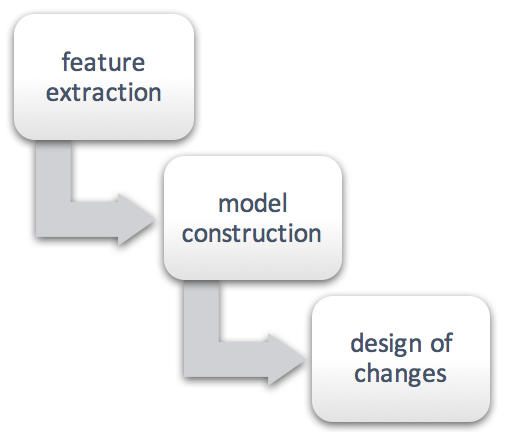
\includegraphics[draft=false,scale=0.6]{images/02-art/oppmodelproc.png}
  \caption{Basic work-flow for designing systems able to implement any kind of modeling of co-existing agents for competitive advantage.}
   \label{behaviorModWorkFlow}
\end{figure}

It is not a secret that in order to be able to increase the likelihood of winning a game one should also consider the extraction of knowledge from opponents in the environment. Opponent modeling \textit{per se} is seen as the attempt to predict and identify behaviors of co-existing adversarial agents and propose appropriate countermeasure actions toward maximizing a given utility~\citep{fathzadeh_opponent_2007}.

In the Robot World Cup Initiative (RoboCup) a body of research has been done in the last decade trying to address the problem of opponent modeling. The RoboCup is a multidisciplinary initiative for building, among other, a team of robots capable of playing soccer. In this scenario, opponent modeling concepts are seen as an important requirement for building a competitive team and also as a growing research topic not only on this domain but also in the more general multi-agent system area~\citep{rofer_overview_2012}. 

Since in most cases game history data is available, researchers have extensively used data mining and~\gls{ml} techniques in order to construct off-line models of opponents which could then be used as classes in a kind of ``prediction phase'' during actual game play. Often, this prediction phase basically means: try to match the current observed opponent behavior to one the existing models for then try to adjust the internal behavior parameters accordingly. This matches the basic work-flow scheme in figure~\ref{behaviorModWorkFlow}.

Some important contribution to the problem has been proposed by~\citep{fix_behavior_2000,riley_recognizing_2002,riley_coaching_2001,riley_planning_2002}. In~\cite{riley_recognizing_2002}, the authors explored the domain of RoboCup by studying how to improve their agent team by constructing a probabilistic model representing predicted opponents' locations given the recent history of ball's movement and initial team members' locations. As common in this scenario, their approach focused in the use of a ``coach'' agent, enabled with a number of predefined models and a centralized view of the world, whose main role is that of communicating a plan to the rest of the team. The big idea is to take into consideration how a model matches the observed data in order to predict the opponent general behavior. 

The main assumption made by the author was that the opponent behavior can be generated from a sample drawn from the predefined set of models given to the coach. Given the predefined models, it is a challenge to decide which model best describes the opponent at run-time. As in the common supervised learning paradigm, they assumed the opponents will behave similarly to how they performed in the past, and use that information to develop a plan. In all of the models used, the distribution of each player's final position was represented by a two-dimensional Gaussian with equal variance in all directions. On successive works~\citep{riley_coaching_2001,riley_planning_2002} the authors managed to improve the online model selection through a kind of Naive Bayes approach focusing on plan representation and execution expressing spatial-temporal relations. 

An interesting observation made by the authors, also pointed out in the work of ~\cite{rofer_overview_2012}, is that during the plan execution it was not possible to take advantage from single unpredictable opportunities that may emerge. For instance, the agents would follow the plan strictly even if there is a clear chance of being successful against the opponent team by taking an immediate off-plan action. It is important to observe how this issue may direct affect the efficiency of an autonomous agent involved in a~\gls{pirg}. It is extremely necessary for the agent to keep a closer loop with the environment, paying attention to every observation that may emerge, as opposed to follow blindly a pre-selected behavior. Naturally, this paves the road for solutions that can represent some degree of belief regarding plan execution and revision. A possible solution to this issue was also pointed out by the authors. They basically suggested to store alternative plans and intelligently add monitors for these plans as in~\cite{veloso_rationale-based_1998} so that they could make the plan execution opportunistic~\citep{riley_coaching_2001,riley_planning_2002,rofer_overview_2012}.

In~\cite{iglesias_comparing_2006} the goal was to use statistical dependency tests for the identification of significant sequences from which to relate states to chains of events. Their underlying assumption was that observed team behavior can be transformed into a sequence of ordered atomic behaviors. In the follow-up work~\cite{burgard_classifying_2008}, sub-sequences inside sequences of behaviors are analyzed by using a frequency-based method. The most relevant aspect presented on their work is that the model of an agent behavior is represented by a distribution of relevant sub-sequences. The behavior classification procedure is done using a modified Chi-square Test.

\cite{steffens_feature-based_2003} studied the application of feature-based models for representing opponent behavior. The gist of this approach is the identification of few features that could be observed by raw sensor data during game play, which diverged from~\cite{fix_behavior_2000} who stored every observation on the model. These features were classified by using a Bayesian method, then a knowledge base is used in order to respond to what has been classified, i.e, select the appropriate strategy. One example of such features were text-based description for in-game situations, like: ``The opponent often does long passes along the left wing to the forwards''. The methodology investigated in the paper was further studied in the context of Case-based Reasoning in~\cite{steffens_similarity-based_2005}. In this follow-up research, Steffens was able to identify some gain in classification accuracy showing that similarity-based opponent modeling could benefit from domain knowledge~\citep{rofer_overview_2012}. Case-base Reasoning, however, is likely to lead to high computational costs given the large number of cases to be retained in a highly dynamic environment~\citep{ahmadi_using_2004,rofer_overview_2012}.

\cite{kaminka_learning_2003} translate observations into a time-series of recognized atomic behaviors. For instance, given a stream of raw observations about the team members' position and orientation plus the position of the ball, their approach would recognize soccer-playing behaviors (passes, dribbles, etc.). Unlike other efforts, they did not care about how the low-level behaviors combine together for generating high-level strategies.  

\cite{ledezma_predicting_2002} also formulates the problem of opponent modeling as a classification task. In tackling the problem they proposed the decomposition of the learning task into procedures: the learning of the action name (passing the ball, kicking), and learning the parameters of the action. A follow-up work~\citep{ledezma_predicting_2005} further studied the subject by implementing~\gls{ml}-based methods to create modules that are able to infer the opponent's actions by means of observation. Their method, was called ``Opponent Modeling Based on Observation'' (OMBO) and was designed to make improvements along two pathways: First, tackling the creation of a generic module (Action Labeling Module) that is able to label the last action (and its parameters) performed by any robosoccer opponent. This happens via the observation of another agent. The justification for this method is that agents generally do not have access to input/output pairs of events generated by other agents. So, the approach must rely on sensor inputs only. Second, the construction of a model of the other agent is based on data acquired from the first module. This is what they called ``Model Builder Module''. In ~\cite{ledezma_ombo:_2009} they further discussed the applicability of the OMBO method giving a proof-of-concept of learning a model of two different goalies. The idea was that their team striker gets as close to the goal as possible, and shoots when the goalie is predicted to move, i.e, by anticipation of the opponent movement. Figure~\ref{OMBO_model_task} presents the holistic view of the method found in~\cite{ledezma_predicting_2005,ledezma_ombo:_2009}. 

\begin{figure}[htp]
  \centering  
  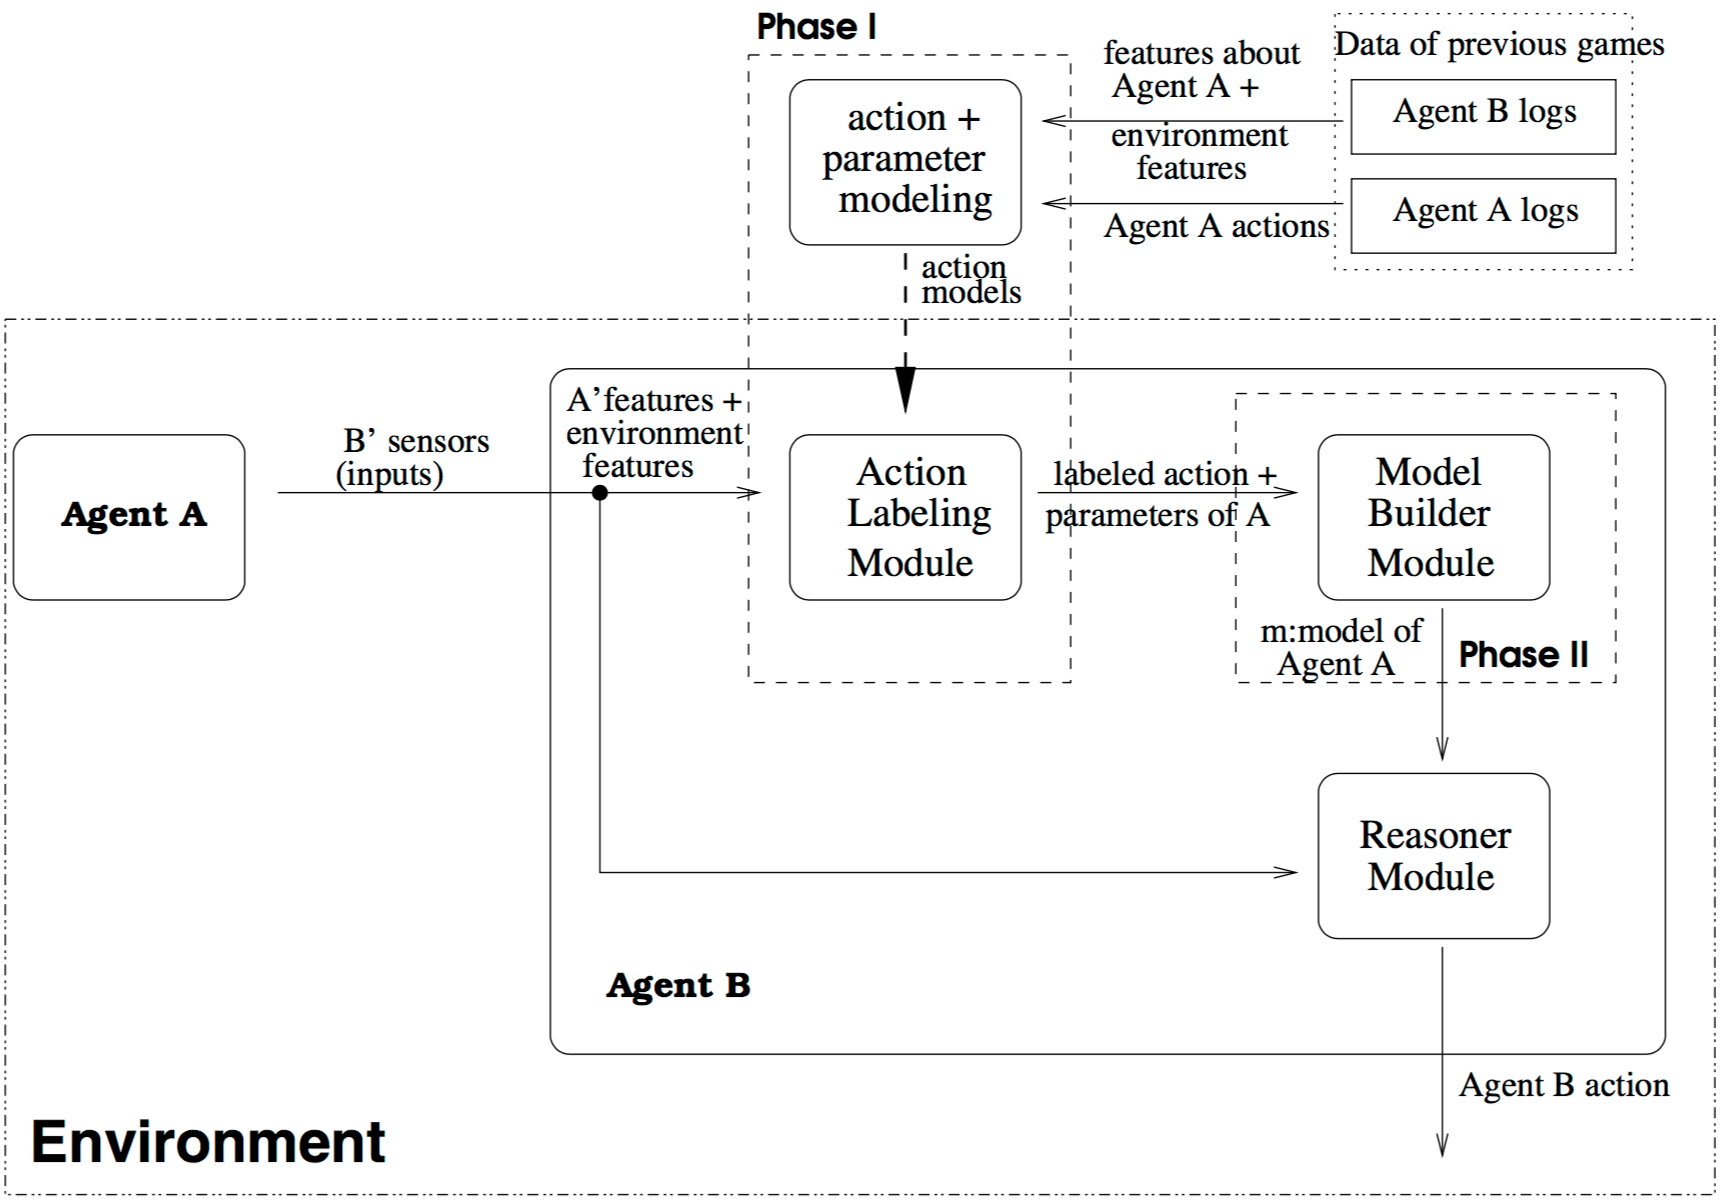
\includegraphics[draft=false, width=\textwidth]{images/04-competition/OMBO_model_task.png}
  \caption{The OMBO model from~\cite{ledezma_predicting_2005, ledezma_ombo:_2009}. The approach is based on two main phases: action labeling and model building.}
    \label{OMBO_model_task}
\end{figure}

Using data mining in order to define models of opponents in an off-line manner is the ideal scenario of an agent learning a model of other agents' behavior via direct observation of their past actions. However, this is only reliable when agents have many repeated interactions with one another or when the assumption of similar behavior between agents holds, otherwise it is hard to obtain any good generalization~\citep{stone_defining_2000}. Given the characteristics of the domain (physical interaction between agents), one may realize that the notion of proximity is quite important\footnote{Proximity is a notion that basically relates to how close/distant are interacting entities. It this turns out to be an ubiquitous notion even in simulated physical interaction as that showed in most videogames.}. Often, authors try to exploit proximity aspects as well as the spatial-temporal relations with certain property of the environment, for instance, the domain an agent exert over a field region (e.g,~\cite{riley_empirical_2002}). Obviously, proximity is not enough, but when combined with other aspects, like timing aspects, it is possible to get good estimates about the behavior of agents in their attitude with respect to in-game tasks. This trend is going to be present on the majority of papers focusing behavioral modeling.

Using the Rush 2008 American football simulator,~\cite{laviersa_using_2014} introduced methods for performing predictions about the players' physical movements when learning team policies. When focusing on recognition of team play they investigated the use of~\gls{svm}, an optimal margin classifier commonly used in supervised learning problems. They trained~\glspl{svm} for a multi-class objective by using a collection of simulated games under controlled conditions, so they got instances of every possible combination of offense and defense plays from a number of team starting formation configurations. The output of the play recognizer was defined as the system's best guess (at the current time step) about the opponent's choice of defensive play. Thus, they could use this information to select the most appropriate offense.

Also in~\cite{laviersa_using_2014}, the authors focused on proposing methods for discovering how to effectively  subgroup agents together so to accomplish a given formation task, similar to~\cite{stone_task_1999}. Here again they based their method on an analysis of game data from successful team plays. The idea was to implement a supervised learning mechanism in order to identify important groups of players in each play. It is interesting to mention the three general types of cues that were used for the purpose of subgroup extraction: \textit{spatial} -- i.e, the constant relationships between team members over a period of time; \textit{temporal} -- co-occurrence of related actions; \textit{coordination} -- dependencies between members' actions. These cues turn out to be basics features for most types of approaches in the discussed scenario.

When tackling team formation, one may observe that a large number of~\gls{ml} techniques have been tested in order to improve countermeasures for a specific team. Again, most of the methodologies use log files for the purpose of off-line learning of relevant characteristics. Neural Networks, for instance, have been extensively used for identifying the position of opponent team members with respect to given preset formations. After identifying a given formation, a plan could be transmitted by the coach agent to the rest of the team all for the purpose of performing the appropriated counteraction~\citep{nakashima_off-line_2010,ramos_discovering_2008, faria_machine_2010, visser_recognizing_2001}.

For a in-depth overview of opponent modeling in RoboCup the reader is invited to refer to~\cite{rofer_overview_2012}. In the work the authors classify methodologies into two categories which basically comprise \begin{inparaenum}[\itshape a\upshape)]\item``formation modeling'', as it stands for the task of modeling team plays under the umbrella of collective behavior, and \item``individual behavior modeling'', which is related to the idea of modeling a single opponent agent\end{inparaenum}.

%TODO You cannot limit this important section to the summary of an old paper reporting older results. I cannot believe there aren't any other approaches to model opponents for competitive advantage.
% EWERTON: I can try to insert more as soon as I solve the other more urgent issues in the text. 

\subsection{Commercial interactive simulated environments}

Virtual games have enabled a large amount of research effort into the design of player modeling methodologies. This is due to the increasing need for making~\gls{npc} believable, i.e, make them resemble human behavior by implementing similar (to human) deductive reasoning process for action selection. In summary, the need of such ability in virtual games is at least due to a few main facts: \begin{inparaenum}[\itshape a\upshape)]\item the growth as a commercial product; \item the increasing complexity; as well as \item the need for developing games that can exhibit a major level of intelligence and adaptation (personalization)\end{inparaenum}~\citep{bakkes_personalised_2012}. 

A growing collection of papers have been published trying to address the problem of predicting the player (opponent) behavior (actions) in different levels and in different contexts. Focusing on opponent modeling, \cite{herik_opponent_2005} presented an overview of efforts for commercial games. In this work, they emphasize types and roles of opponent models, such as ``speculation'', ``tutoring and training'' as well as ``mimicking characters''. In ``speculation'', the idea is that some kind of heuristic (or utility function) -- such as minimax in zero-sum games like chess or checkers -- is used in order to assess the quality of available opponent's actions during game-play. In simple terms, this relates to the idea of using knowledge of the opponent's preferences or skills in order to drive the game into positions/states that are considered to be \textit{less favorable} to the opponent. This is the same core idea behind the approach described in~\cite{markovitch_learning_2005}, where they defined the concept of \textit{opponent weakness} (as a quantifying measure) together with a method for learning a model of this concept. The key-point in~\cite{markovitch_learning_2005} was the care about the potential harm of modeling error and the incorporation of their concept as an extra feature in the decision process, not as the core itself.

Another example of such modeling type is the research done by~\cite{missura_online_2008}, where the authors propose to rank available actions for the player (at each turn of the connect four game) to find a way to balance the behavior of the computer-controlled agent to that of the human player. The aim was to estimate the player's expertise, when looking at the history of moves performed, and by assessing their quality (rank) based on a minimax approach.  Thus, at each turn, they could make their agent select only actions that have similar rank to that of the player\footnote{Despite the fact~\cite{missura_online_2008} is mentioned here as a ``speculation'' type of opponent modeling -- since there is a kind of simulation procedure for evaluating the player's quality of movement -- one may also see this work as an effort for tailoring the game for optimizing gaming experience, i.e., a kind of difficult adjustment approach.}.

Tutoring and Training is seen in~\cite{herik_opponent_2005} as a type of opponent modeling that has to do with the assistance of a human player. For instance, a model of the human opponent may be built as to teach him how to achieve certain in-game goals in a personalized manner. This is ideal for \textit{serious game} environments where the player is confronted with a simulation of real-world events while trying to solve a potential real-world problem. Even by knowing that serious games can be entertaining, in this scenario the main purpose is essentially to train or educate users, thus, coming up with models that support the game steering behavior towards those aspects that are definitely important. In this context, \cite{ha_goal_2011} tried to identify player's goals in the Crystal Island game -- a non-linear educational game about microbiology -- by using Markov Logic Networks\footnote{A probabilistic technique comprising a set of weighted first-order logic \textit{formulae} that enables uncertain inference over Boolean logic. }. Goal recognition is assumed to be an important piece for player modeling and generally tries to identify the user's goals from a set of low-level observation (abduction)\footnote{Also related to goal recognition are techniques like plan and activity recognition, both well-known problems in general~\gls{ai}~\citep{ha_goal_2011}.}. 

The study in~\cite{ha_goal_2011} follows previous work on goal recognition (such as~\cite{mott_probabilistic_2006}), but under a much broader view, that of having individual goals not independent from each another (which turns goal recognition into a classification problem) and that of having ambiguous causality effect between actions and goals. In terms of features for player actions, they targeted three properties: \textit{action type} (e.g, moving to a place), \textit{location} (game place where the action was taken), \textit{narrative state} (player's progress in the game narrative).  Once again, model parameters are learned from corpus of data collected from the environment. Their results were compared with two baselines based on \textit{unigram} (a model that predicts goals based on the current player action) and \textit{bigram} models (makes prediction based on previous action as well) obtaining a 82\% improvement over them.

In~\cite{herik_opponent_2005}, the ``mimicking characters'' type is said to correspond to the observation that the virtual game is designed to be fun and entertaining, as opposed to play as strong as possible all the time. This amounts to the well-known observation that when performing a companion role, for example, the agent must do what is possible to behave in accordance to the expectation of the player, otherwise the human may lose interest in the game. Thus, this requires a model of the human in order to be effective. Also, in a~\gls{pirg} scenario, this is an important aspect that would enable advancements in the interaction as a whole since the behavior of an autonomous agent should be dynamic enough to adjust to the individual experience. The central point is that of not designing static behaviors that are likely to be exhaustively exploited by the player. This type hugely overlap with the ideas of player modeling for creating a balanced game play, i.e., adjusting the game for the player individual experience. This subject is brought back on section.  

Often, games and simulations provide access to full-observability of in-game events and player's actions. When this is not true, there may be a (often large) corpus of data from usage history that is available for information extraction. This, naturally favors the use of off-the-shelf data-mining algorithms that can be easily set up and tested multiple times. However, on the design of~\gls{pirg}, specially on a brand-new project, one may suffer from the lack of data for constructing off-line models of players. To get around this problem there exist at least two main alternatives: \begin{inparaenum}[\itshape a\upshape)]\item setup a data collection procedure, for example, by designing a first version of the game, implementing it and then collecting data in order to refine the game design; or \item invest on online procedures that are able to extract features from the player and come up with models of player behavior on run-time\end{inparaenum}.

In~\gls{pirg}, it should be possible to design methods that account for the evaluation of the current state in order to know what are the corresponding chances of winning/losing at the moment, allowing for planning ahead how to overcome/support in case of need. However, it is worth to take into account the general constraints perceived in the domain, such as computing complexity, mobility and perception constraints. 

Moreover, there is to consider that computation in~\gls{pirg} should be supported by low cost platforms only, which have limitations in computing power, energy consumption and other.

\section{Considerations}
In this chapter we have described the concepts behind our platform's ability to play competitively,~\ie to select actions aimed at winning the game. We have kept this goal separate from that of modeling player for the purpose of entertainment maximization, and of driving the robot behavior towards this, since we view the two goals as often conflicting. While ideally we search for a robot that is able to act rationally under the later objective, it should also provide means for competitively engaging the player and obey the game rules. In theory, the robot should tend to balance its chances of winning the game with the player's ones. However, it should not do that in a way that can be interpreted by the player as ``letting'' him win. Therefore, in our experiments we decoupled the two styles of playing in order to easy tackle each style issues and concerns individually. For all factors, our work assumed the robot's ability to play the game well enough to be perceived as a competitive agent and we did not deal much with this dimension. This assumption was confirmed in the self-report given by players after the game. In the next chapters we present the contributions of our research in modeling the player for entertainment maximization.

\part{Engagement design}

\chapter{A review on player modeling for experience optimization}\label{ch:review_playing_optimization}
In virtual games, player modeling is best defined as the study of the use of artificial and computational intelligence techniques for the construction of models of players in dimensions regarding behavior, cognition, and affective states as well as beyond-game high level aspects spanning personality and cultural background~\citep{yannakakis_player_2013}. The idea behind such models is related to the goal of enabling a game to adjust the capability of its components and attributes towards an individual player satisfaction~\citep{herik_opponent_2005}. This idea has largely increased in importance over the last years. As one of the central reasons for that, is the increasing complexity of modern games fostered by the enhancement in computing power and graphics, as well as the commercial strategy of personalizing gaming experience~\citep{teng_customization_2010, herik_opponent_2005}. This chapter presents a brief overview of works targeting experience optimization, organized in three main parts, focusing on different aspects related to play experience optimization, namely: \textit{cognition}, \textit{behavior} and \textit{affection}. A relationship between our work and what proposed in literature is also presented.

\section{Focus on cognition and theoretical models of behavior}
One way researchers have addressed player modeling in games is by relying on theoretical frameworks mainly supported by psychology and neuroscience factors~\citep{yannakakis_player_2013}. By doing so, cognition aspects -- broadly seen as a set of all mental abilities and processes related to knowledge, such as: attention, memory, evaluation, reasoning, problem solving and decision making, learning and so forth -- are often investigated. 

Researches focused on theoretical framework of behavior are described in~\cite{yannakakis_player_2013} as being model-based. In this sense, they follow the \textit{modus operandi} of Humanities and Social Sciences which work, according to the authors, by coming up with a hypothetical model in advance, and investigate to what extent it fits the observations. When concerning the development of engaging experiences in entertainment systems,~\cite{yannakakis_how_2008} states that a comprehensive review of the literature regarding the elicitation of qualitative features and criteria derived from experimental psychological studies reveals a tendency of overlapping with the exploitation of theories of \textit{fun}, such as those discussed in~\cite{malone_what_1980},~\cite{lazzaro_why_2004} and~\cite{koster_theory_2013} envisioning to drive game design, as well as \textit{flow}~\citep{csikszentmihalyi_flow:_1991} (often used as a way of evaluating player enjoyment~\citep{sweetser_gameflow:_2005, cowley_toward_2008} (Fig.~\ref{flowDiagram})) and concepts like \textit{immersion}~\citep{calleja_digital_2007}. Most acceptably, according to theses theories and concepts, player engagement is most related to factors such as challenge, curiosity and fantasy.

\begin{figure}[htp]
  \centering  
  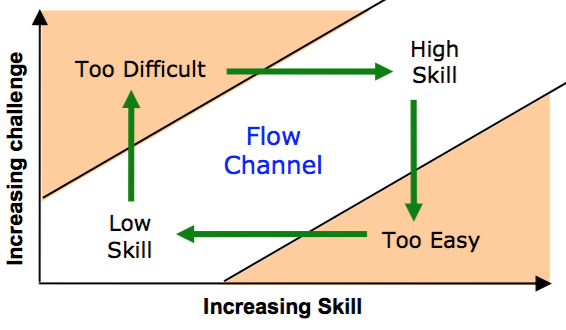
\includegraphics[draft=false]{images/02-art/flowDiagram.png}
  \caption{A flow diagram from~\cite{hunicke_ai_2004}. The figure shows the relationship between skill and level of challenge derived from the theory of flow~\citep{csikszentmihalyi_flow:_1991}. The point is to keep these two dimensions in a kind of positive correlation, meaning an increase that roughly approximates the diagonal.}
  \label{flowDiagram}
\end{figure}

Models aligned with cognition theories are seen as a valuable opportunity for understanding what the user is thinking when playing, which has direct relation with the ultimate desire of making the game respond intelligently to the player. According to~\cite{bohil_cognitive_2007}, the fundamental advantage of a direct focus on modeling principles supported by a theory of cognition is that it provides dynamic view at the individual player level, since it is possible to make statements about attention, learning, decision strategies, biases, an so on, unraveling indicators of the mental underpinning of observable behavior. 

The design of better~\gls{npc}s, for instance, is one of the central areas positively affected by the focus on cognition~\citep{funge_ai_1999}. Intuitively, once it is possible to measure some cognitive-related characteristics in the player (e.g., the attention level with respect to some in-game resource) it is possible to use them to steer the~\gls{npc} behavior towards the improvement of a desired~\gls{ai} capability -- Adaptive difficulty adjustment is one of these capabilities. Indeed, game difficulty is seen as having a direct link with challenge and fun, acting as source of satisfaction~\citep{koster_theory_2013,yannakakis_modeling_2006}. 

Cognitive models of players were also investigated with respect to psychological and cognitive neuroscience motivated question trough assessing physiological and/or psycho-physiological states during play. For instance, brain imaging techniques have been used to understand brain activity patterns related to aggressive thought stimulated via violent game content ~\citep{weber_does_2006}. The work of ~\cite{baumgartner_neural_2006} used Electroencephalography (EEG) combined with psychometric measures, as a first attempt to investigate neurophysiological underpinnings of spatial presence\footnote{spatial presence is considered as a sense of being physically situated within a spatial environment portrayed by a medium, such as television and virtual reality.} triggered in different virtual roller coaster scenarios.

Optimistically, as seen in~\cite{bohil_cognitive_2007}, the major point in cognition or related framework-based approaches for player modeling is to discover which model inputs -- in the sense of a parametric representation of cognition aspects -- place, for instance, unrealistic demands on a specific cognitive function, such as attention. Successful results on this, might heavily equip researches and game developers with valuable guidance for narrowing the range of necessary resource-consumption when aiming for desired results.   

\section{Focus on in-game actions, and behaviors}\label{sec:in_game_action_reviews}
A classical trend in player modeling is to investigate how primitive in-game activities can be used to describe the general behavior of the player. Originally, the first attempts for modeling players in this context used classical zero-sum board games (like chess, checker and go) as test-beds mainly by implementing search/heuristic methods to find the best moves in the game-tree. According to~\cite{bakkes_player_2012}, since tree-search techniques use evaluation functions in order to assess the pay-off of a particular move, they may be considered player models.

In-game actions are building blocks for any standard behavioral modeling approach. Most commonly, primitive actions are the unique way to identify player's preferences and decision-making style. Additionally, this modeling dimension is transferable across different game genres. A sequence of low-level actions -- such as moving from one direction to another -- is generally related to a classifiable behavior, such as ``attacking'', ``defending'', ``fleeing'', etc. In the RoboCup soccer league, for instance, a sequence of actions 9including targeted movements towards the opponent goalie may be commonly (and generally) classified as an ``attack''. Similarly, a sequence of actions intending to systematically prevent the opponent team from advancing on the field may be characterized as a ``defensive'' behavior. From this example, it is quite natural to realize that actions encode behaviors by perhaps acting as a kind of representation language for them. The important bit is that by keeping track of performed actions it is possible to find patterns that can be reasonably grouped together under the concept of a specific behavior. As discussed, actions were providing the raw information in most modeling approach for competitive advantage in section~\ref{compadvantage}.

Although classifying behaviors in this way may be relatively easy for simple, fully observable environments that involve a few possible deterministic actions and abstract behaviors, this classification process is limited in modern complex games since they normally have a large state-action space. Moreover, often behaviors lack the existence of a clear crossing point between them, and this makes the construction of player models even more challenging. Giving the size of the state-space, researchers have also to deal with the uncertainty involved in the fact that different action sequences may be related to the same behavior, while having a close relation with others. The fact that action sequence detection may be noisy is important, and also a challenge that has to be taken into account when using low-level actions to model behavior.  Furthermore, while computational constraints (such as memory demand) are the big key point, for instance, in search methods applied to turn based games, the dynamic characteristics in other types of games is the key. In~\gls{pirg}s, the inherent dynamism of the environment demands a special treatment of these aspects.

Besides all computational constraints involved and discussed in the previous paragraph, one might also see  the necessity of having different levels for behaviors. For instance, one might be interested on identifying when the player is mindless attacking, or when the player is using a full-fledged plan for performing the attack. In this context, what is the characteristic that separates these two behaviors? Again, using the RoboCup soccer league as an example,~\textit{is the player engaged in a proper ``attack'' or just keeping the ball in the attack field perhaps for the purpose of spending time?} Note that a ``proper'' attack may have more structured actions, perhaps including well-known patterns as opposed to a behavior of just ``spending time'', which in this case may use different sequences of actions.

The work of~\cite{bakkes_player_2012} presents an extensive discussion about the use of actions for player modeling, envisioning game experience optimization. In the authors' understanding, action models seem to be an attractive possibility for a model, since, once being able to predict accurately the future action that the player will take, acting accordingly would be a relatively easy task. However, they agree that the use of such models are limited unless when applied to relatively simple games. The justification for this is also related to the complexity of state-action space in state-of-art games. The authors also deem three more subdivisions for the topic, reported on Table~\ref{actionModels}.

\begin{table}[!ht]
\centering
\caption{The classification proposed by~\cite{bakkes_player_2012} for dimensions used in player modeling techniques based on virtual in-game actions.}
\label{actionModels}
\begin{tabularx}{\textwidth}{|c|X|} \hline
\textbf{Type of model}&\textbf{Brief description}\\ \hline
Tactic-based & relates to the automatic identification of short-term behavior as composed from actions targeting the achievement of a specific local goal. A common well-exploited concept is \textit{formation of game characters} which can be defined as a disposition of certain game agents.\\ \hline
Strategic-based & concerns global-term game behavior assessed via tactics sequences. This behavior may span over the entire game, some iterations of it or even across distinct genres of games.\\ \hline
Profiling-based & concerns psychological motivation for tactics and strategies.\\ \hline
\end{tabularx}
\end{table}

The divisions presented in Table~\ref{actionModels} are, in fact, not mutually exclusive and one can see them in a loose hierarchical manner. In other words, tactical-based models depend on action-based ones and, in the same way, strategy-based models may comprise a behavior inferred with the help of the previous two, etc. The main advantage, of modeling tactics over actions, however, is that the state-space complexity decreases as a result of higher information abstraction. But, since they are interrelated with each other aiming to achieve an overarching goal, modeling tactics alone, according to the authors, is not enough for effective player behavior modeling, since strategic play assumptions, as a high-level motivation for tactics, is commonly not incorporated, therefore, these models cannot generalize well over the underlying intentions behind observed tactics.

Additional to the use of actions in the modeling context discussed in section~\ref{compadvantage}, they are also the raw material exploited on designing games that can adjust difficulty automatically in order to keep the player's engagement at a high. Specifically, along-side procedural content generation -- the concept of generating game content on the fly --~\gls{dda} has taken a large piece of the virtual game community.

In essence, the idea is pretty simple: start by measuring the player's skill or level of challenge (difficulty) at a given moment and, based on this, steer the game behavior towards a state much likely to be compatible (in skills or challenge level) with that of the player. Following this recipe,~\cite{andrade_online_2004, andrade_extending_2005} aimed at investigating the usage of Q-learning and a challenge function in a 2D fighting game scenario. In their work the authors came up with a challenge function strictly based on the difference between the~\gls{npc} and player's health. From this, a game is assumed to be balanced if the function fluctuates around zero. By using a regular Q-learning they get to choose different best actions so to force the algorithm to choose the ones that most likely, according to the challenge function, matches the perceived player skill. 

~\cite{hunicke_ai_2004}, in turn, addressed~\gls{dda} by considering the notion of inventory analysis, that is, the processes of analyzing what resources are immediately available to the player w.r.t. the current challenge level of the game. During the game process, they observe certain player's characteristics, for example the level of damage the player takes, in order to generate an indication for the necessity of system intervention. When needed, their system would adjust supply and demand or resources so to control overall game difficulty. Ideally, the authors target the reduction of necessary intervention so to make it as seamless as possible. The system aims at keeping the player at the flow channel~\citep{csikszentmihalyi_flow:_1991} by encouraging certain events to take place or not. For example, the system basically tries to predict when the player is repeatedly putting himself on a state where current means can no longer achieve global or local goals.
When this happens, the system intervenes helping the player to progress.

Not surprising, the notion of having a ``challenger function'' that helps to guide adaptation is pretty much ubiquitous in the adapting game literature. Furthermore, any system relying on~\gls{dda} should also be concerned about the timing implication of such technique, i.e., the implications regarding the good moment to perform an attempt towards adjusting the game. For beginners, this is because a high frequency of adaptation is more likely to give the appearance of instability and so cause the game to be perceived as random. This instability is often referred to as the ``rubber-band'' effect as the IA appears to wobble around its skill level if the (human) player is too good and, conversely, overrun the player when he plays equivalent to the~\gls{ai}. Here though, appears clear the difficulty involving designing challenger functions. In the experiments done by~\cite{hunicke_ai_2004}, the authors noticed that a reactive approach, i.e. adjustment of onset elements, may run the risk of disrupting the player's sense of disbelief contributing to make the interpretation of the game harder and also make it ``schizophrenic''.%TODO the previous paragraph seems related to adaptation more than to player modeling. It is a further step possibly deserving a section per se, if you have collected enough info.
%EWERTON: But this section is dedicated to modeling for adaptation, i.e., to experience optimization.

In~\cite{hagelback_measuring_2009}, the authors went further on pooling people's opinion for the sake of knowing if playing an even game is more entertaining over being superior all the time. On their case study 60 people participated and they took the opportunity to conduct experiments using static and dynamic agents for their game test-bed. The dynamic agent type was able to react to in-game player behavior (for instance, to the player losing game resources). The obtained results suggested the dynamic agents were providing most entertainment to players during play while static ones presented themselves as too easy or too difficult. The authors' research provided good evidence for the implementation of~\gls{dda}-based systems.

\cite{spronck_-line_2004} propose one of the most popular examples of player modeling in virtual games. In their method, called ``dynamic scripting'' and defined as an unsupervised online learning technique for games, they maintain several rule-bases, one for each class of computer-controlled agents. Rules in the bases are manually designed using domain-specific knowledge and every time a new agent of a particular class is generated, the rules to compose the agent script are extracted from the corresponding rule-base. In this approach, the probability that a rule is selected for a script is proportional to the weight value that is associated with the rule. Also, the rule-base adapts by changing the rule weights to reflect the success or failure rate of the associated rules in scripts. %TODO Adaptation? EWERTON: in 

It did not take long until researchers realized that using a challenge function would pave the way for black-box optimization algorithm. Much of the literature covers the attempt of using evolutionary techniques as the main technique for~\gls{dda}. Among these works, it is worth notice that of~\cite{olesen_real-time_2008}, where the authors use evolutionary techniques to evolve agents so to balance an estimated challenge rating for the player skill. The take-away idea is that of making agents with a minimal difference in skill (w.r.t the player) to survive more and, on the other hand, lower the fitness of the ones whose difference is larger.%TODO Adaptation?

~\cite{demasi_-line_2003} focused on the use of~\gls{cea}s  proposing some methods and strategies for online evolution in an action (real-time) game. In this game, the~\gls{npc}s is evolved towards improving difficulty levels. The author presents four different methods: one that uses game specific information; one that merges offline-evolved data with online evolution; two others that focus on using online data only and using offline and online data together. Considerable drawbacks in the approach are the slow learning rate and the one-direction way of evolution, always toward the optimizing behavior. %TODO Adaptation? EWERTON: 

\cite{sejrsgaard-jacobsen_dynamic_2011} took a different approach by using~\gls{bt}, a kind of hierarchical finite state machine for controlling~\gls{npc}s, in order to dynamically adjust the difficulty in a 2D fighting game. They basically tested two different approaches. First, the traditional approach of defining predefined behaviors (encoded on~\gls{bt}s) and finding a way to switch between models (behavior) at run-time. For this, they developed an algorithm for selecting~\gls{bt}s based on perceived conditions. The second method, however, adjusts difficulty by changing~\gls{bt} properties themselves at run-time, such as the probability associated with children of selector nodes. This last method, was the one that obtained high capability in balancing the game. As claimed by the authors, their method served as a proof of concept for a small sized scenario (simple 2D fighting game) leaving the possibility for further investigation in larger game scenarios. Here, pops out an opportunity for testing on a~\gls{pirg} context, perhaps by following the current trend on applying such technique in robotics~\citep{scheper_behavior_2015, pereira_framework_2015, marzinotto_towards_2014}. %TODO Adaptation?

In summary, approaches addressing~\gls{dda} must, before the definition of the challenge function, identify important game characteristics affecting game difficulty, and challenge level. The overall philosophy is the adjustment of the game behavior to the perceived player's game skill, which should be made as seamless as possible. A good survey about adaptation-related challenges in games and simulations could be found in~\cite{lopes_adaptivity_2011}. The reader may refer to it in order to see a deeper treat on the identification and discussion of main challenges associated with the domain and also promising directions for research. %TODO Adaptation!

\section{Focus on affection aspects}\label{affectmodeling}
Also, some trend has emerged aiming on assessing the player's affective state (mainly emotion) as a mean of measuring the quality of interaction provided by the game. Here, the goal is related to the task of inferring internal traits of the player, such as personality and preference, during game-play~\citep{van_lankveld_psychologically_2009}. Methodologies that take this approach are more towards a research domain known as \textit{affective user modeling}, where the key point is that of assessing, heavily by using affection models, the inner state of the player regarding motivations for actions either based on action selection or through physiological data~\citep{van_lankveld_psychologically_2009}.

Being able to identify emotional profiles in this domain is useful given that they target a direct characterization of enjoyment level. For instance, after realizing that the player is compatible with an extroverted and highly responsible profile, the game~\gls{ai} may engage the user in rapid and repeated shifts of events, like from calm situation to a long and intense chain of events, or even a steep increase on motion abilities for~\gls{npc}s agents when proximity aspects, for instance, are important~\citep{bakkes_player_2012}.

Working on this,~\cite{tognetti_modeling_2010} proposed a framework to estimate player enjoyment preference from physiological signals in a car racing game. They collected 5 physiological signals from players, namely:~\gls{bvp},~\gls{ecg},~\gls{gsr}, Respiration (RESP) and Temperature (TEMP). From these basic signals, they were able to extract features such as: Heart rate (from ECG and~\gls{bvp}); magnitude and duration of~\gls{gsr}; expiration/inspiration time, apnea in/out time, respiration interval (all three from RESP); upper/lower envelope of~\gls{bvp}. Their data analysis, using Linear Discriminant Analysis, showed correlation between reported enjoyment and the described features, motivating further application on the use of biological signals without making any assumption on players' in-game activity.

Yannakakis and Hallam have published lots of papers on the matter of capturing and modeling affective state of entertainment, targeting children physiological state during physical game play. In~\cite{yannakakis_modeling_2006} and \cite{yannakakis_entertainment_2008}, children's heart rate, blood volume pulse and skin conductance were analyzed in the Playware prototype playground~\citep{lund_playware_2005}. Their findings suggested that a higher average and maximum heart rate, a steeper blood volume appear to correlate with higher levels of reported entertainment in children of 8-10 years-old. Essentially, the main effort is related to modeling entertainment based on selecting a minimal subset of individual features that are able to construct the quantitative user model for predicting the children's reported entertainment preferences. In doing so, they tested large margin algorithms (based on the~\gls{svm} principle) and Evolving Artificial Neural Networks. Successive works investigated feature selection and extend the approach for computer games~\citep{yannakakis_towards_2006,yannakakis_entertainment_2007,yannakakis_feature_2007,yannakakis_entertainment_2008-1}. 

There are indeed plenty of papers proposing the use of physiological data in game research. A widespread understanding is that measures from these methods are known for providing sensitive ways to assess the game experience, but they are hard to deal with since very often they require controlled experiments. In order to know more about this trend of research, the reader may refer to~\cite{kivikangas_review_2011} whose work presents a review focused on psycho-physiological methods for game research. For what concerns~\gls{pirg}s, physiological data are affected also by physical activity, thus behavior or emotion modeling based on these data could be negatively affected by the intrinsic way of playing this type of games.   
 
\section{Existing review papers and taxonomies}\label{reviews}
Taxonomies and reviews for player modeling have been recently proposed. \cite{smith_inclusive_2011} state that ``player modeling'' is a lose concept, since it can equally apply to everything from a predictive model of player actions resulting from machine learning to a designer's description of a player's expected reactions in response to some piece of game content. The authors introduced a broad taxonomy for the purpose of distinguishing between the major existing player modeling applications and techniques. Four facets were suggested: the scope of application, the purpose of use, the domain of modeled details, and the source of a model's derivation or motivation. The expectation involved is that the taxonomy would allow the identification of relevant player modeling methods for particular problems and clarify roles that a player model can take. As pointed out in the previous section, the work of~\cite{bakkes_player_2012} focuses on player behavioral modeling via in-game measurement of the human player distinguishing four types of player models: tactical models, strategic models, and player profiling. %TODO In the table 5.1, they were only 3, action models missing. Try to be consistent.
Through their examination, they noticed that these models are increasingly resource-intensive to build, but they also have an increasing tendency to generalize better.%TODO better than what?

\cite{machado_player_2011} also proposed and discussed a taxonomy for player modeling research gathering and organizing information from several different sources. They, in turn, tried to characterize the most important topics in the area expanding the discussion from~\cite{herik_opponent_2005} about the most common techniques, further presenting a new set of techniques. Additionally, they did an analysis of player modeling research possibilities in several game genres and also listed suitable game platforms for experimentation, discussing main characteristics.

Targeting a holistic view of player modeling with the aim of providing a high level taxonomy and discussion of key components of a player model,~\cite{yannakakis_player_2013} cluster the field into either \textit{model-based} approaches -- those that are built on a theoretical framework -- or \textit{model-free} ones -- those that refer to the construction of a model between player input and a player state representation by mainly relying on the \textit{modus operandi} of exact science, through computational techniques related to~\gls{ai} and~\gls{ml}. Additionally, they present a discussion about inputs and outputs to computational methods described as well as applications and current key challenges the field faces which are correlated to the inputs and outputs for the mentioned computational models.

\begin{table}[!ht]
\centering
\caption{Summary of existing popular survey-like papers concerning player modeling. {\mycirc} stands for proposal of taxonomy, {\mystar} stands for overview of literature and {\mydtriangle}, in turn, correspond to survey or review.}
\label{summaryReviews}
\begin{tabularx}{\textwidth}{|c|c|X|} \hline
\textbf{Paper}&\textbf{Type}&\textbf{Brief description}\\ \hline
\cite{smith_inclusive_2011}	& {\mycirc} & Build a broadly applicable taxonomy that can describe player modeling techniques across all games , both digital and non-digital, and in all games genres.\\ \hline
\cite{bakkes_player_2012} 	& {\mycirc} & An overview of methods by detailing four distinct approaches for modeling behaviour of players, namely: modeling player actions, modeling player tactics, modeling player strategies and player profiling. \\ \hline
\cite{yannakakis_player_2013} & {\mycirc},{\mystar} & A holistic view of player modeling, a high level taxonomy and discussion of key components as well as a description of challenges currently faced in the topic.\\ \hline
\cite{bakkes_personalised_2012} & {\mystar} & Motivation concerns for the topic, an broader overview, and  adaptive components for personalised games\\ \hline
\cite{machado_player_2011} &{\mydtriangle},{\mycirc} & Presents a survey of the field, discussing the main concepts and proposing a general taxonomy. \\ \hline
\cite{karpinskyj_video_2014} & {\mydtriangle} & Highlight most relevant trends and directions of research for the task of designing personalisation in games.\\ \hline
\end{tabularx}
\end{table}

Focusing on the point of personalized game experience in general,~\cite{bakkes_personalised_2012} provides a motivation for the promotion of methodologies in the topic as well as an extensive overview of scientific literature. To the former objective, they describe psychological foundations, the effect of satisfaction, the advantages to game development and requirements for achieving ambitions. To the extent of the overview, they go pretty much in the same direction of what has been exposed in~\cite{bakkes_player_2012}, however providing an intensive discussion about \textit{components of personalized games}, namely: space adaptation, mission/task adaptation, character adaptation, game mechanics adaptation, narrative adaptation, music/sound adaptation, player matching and difficulty scaling. An additional discussion about the relationship between personalized gaming and procedural content generation as well as the generalization to other domains (such as ambient games, human-computer interaction) is also mentioned.

Similarly, the work of~\cite{karpinskyj_video_2014} touches the subject of surveying the most relevant trends and directions of research in personalisation of computer games, to the extent that it is a true multi-disciplinary problem requiring contribution from areas as diverse as artificial and computational intelligence, game studies, psychology, game development and human computer interaction. Their survey considers five dimensions enabling to distinguish players from each other: preference, personality, experience, performance, and in-game behavior. Their discussion also aims to identify key research avenues that require further exploration. Table~\ref{summaryReviews} summarizes the most important points in the mentioned papers. 

Competitive advantage and/or experience optimization (section~\ref{ch:review_playing_optimization}) 
are not the unique types of approaches. There were also attempts for classifying opponent behavior to support the design of the game itself. An example of this is the work of~\cite{etheredge_generic_2013} where it is possible to see the implementation of fuzzy cluster analysis and~\gls{hmm} for finding player styles. %TODO Shouldn't this stay in player modeling section? Why is it here, in the "review papers" section?
The approach works as a classification method for player behavior, defined as a sequence of game actions. It consists of three components: interaction registry, cluster analysis and~\gls{hmm}. The first, serves as a data storage for actions maintaining a cumulative score value for them. The idea behind this is that actions that are not frequent are going to have an exponentially decreasing value in importance. On the other hand, frequently used actions have high importance score. These importance values for actions then constitute a primary source of information that is going to be used by cluster analysis as a way to group, i.e. classify, the player's styles.~\gls{hmm} is then used during game-play aiming to classify new players, as they play, and helping to spot appropriate and dependent game adjustments. The author claimed their method would be able to be used across different games (given their definition of player behavior) which can be considered as a possible generic design tool.

%TODO the same comment holds for the following one
Using the Rush 2008 American football simulator,~\cite{laviersa_using_2014} introduced methods for performing predictions about the players' physical movements when learning team policies. When focusing on recognition of team play they investigated the use of~\gls{svm}, an optimal margin classifier commonly used in supervised learning problems. They trained~\gls{svm}s for a multi-class objective by using a collection of simulated games under controlled conditions, so they got instances of every possible combination of offense and defense plays from a number of team starting formation configurations. The output of the play recognizer was defined as the system's best guess (at the current time step) about the opponent's choice of defensive play. Thus, they could use this information to select the most appropriate offense.

%TODO the same comment holds for the following one
Also in~\cite{laviersa_using_2014}, the authors focused on proposing methods for discovering how to effectively  subgroup agents together so to accomplish a given formation task, similar to~\cite{stone_task_1999}. Here again they based their method on an analysis of game data from successful team plays. The idea was to implement a supervised learning mechanism in order to identify important groups of players in each play. It is interesting to mention the three general types of cues that were used for the purpose of subgroup extraction: \textit{spatial} -- i.e, the constant relationships between team members over a period of time; \textit{temporal} -- co-occurrence of related actions; \textit{coordination} -- dependencies between members' actions. These cues turn out to be basics features for most types of approaches in the discussed scenario. Undoubtedly, a larger number of papers focused on player modeling for improving playing experience as to maximize the chances of maintaining the player engaged. 
%TODO To eliminate, I imagine -> This is the topic of discussion of the next section.

\section{Our work and the literature}
In accordance with what exposed so far, our research concentrated the aspects of playing for entertainment maximization aiming at developing new strategies for supporting acceptability of~\gls{pirg}s. To what concerns the literature, we define our work as related to the application of latent~\gls{ml}-model-based approaches %TODO Do I have missed this term in the classification? If you refer to the chapter just above, you should use the same classification terms.
to the problem of modeling the general behavior of a player. 

Our work concentrated on the exploitation of classification and clustering to differentiate among players. We have focused on modeling physical behavior and show how such aspect of interaction can be used to achieve player categorization and eventual robot adaptation. In terms of the related works presented above, we tend to be related to approaches that model the in-game activity as those presented in section~\ref{sec:in_game_action_reviews}. The main concerns in this phase are depicted in the conceptual relationship in the graph in figure~\ref{graph:ENGAGEMENT_structure}. %TODO It has to be clear to us, and to the reader, that ENGAGEMENT IS NOT ENTERTAINMENT. A part the problems in the correct and formal definition of the two terms, which should be provided, we cannot just assume that engaged people is also enjoying the game. For sure if engaged, he is motivated to play

\begin{figure}[ht]
    \centering
    \begin{tikzpicture}[ every annotation/.style = {draw,
                         fill = white, font = \Large}, scale=0.75,transform shape]
                         
      \path[mindmap,concept color=black!40,text=white,
        every node/.style={concept,circular drop shadow},
        root/.style    = {concept color=black!40,
          font=\large\bfseries,text width=10em},
        level 1 concept/.append style={font=\Large\bfseries,
          sibling angle=60,text width=7.7em,
        level distance=15em,inner sep=0pt},
        level 2 concept/.append style={font=\bfseries,level distance=9em},
      ]
        node[concept, font=\fontsize{16pt}{17pt}\selectfont\bfseries] {Engagement\\ Optimization}
        [clockwise from=0]
        child[concept color=green!50!black] {
          node[concept] {Player\\Modeling}
          [clockwise from=90]
          child { node[concept] {Behavior} }
          child { node[concept] {Learning} }
          child { node[concept, scale= 1.2, font=\fontsize{7pt}{17pt}\selectfont\bfseries] {Engagement} }
        }
        child[concept color=orange] { node[concept] {Difficult\\Selection}
        child { node[concept, scale=1.5, font=\fontsize{7pt}{17pt}\selectfont\bfseries] {Deception} }
        };
    \end{tikzpicture}
    \caption{Some relevant concepts in the engagement optimization dimension for our ~\gls{pirg} agent.}
    \label{graph:ENGAGEMENT_structure}
\end{figure}

Player modeling here takes into consideration several aspects like the general behavior (usual in-game actions), learning curve (changes in the usual behavior) and engagement (direct modeling of engaging variables). 

For all effects, we concentrated on tackling the general behavioral aspects so as to avoid the complexity of modeling dynamics. However, as one can see, the latent modeling algorithm we use can be easily extended to allow for modeling dynamics. This is in fact a direction of future work.

Additionally to modeling the player, we also investigated the advantages of implementing deceptive navigation and how this relates to self-reported game acceptability. The results indicate the need to further explore the concept and to isolate variables that can make the player perceiving the deceptive behavior. 
\chapter{Activity Recognition in RoboTower 2.0}\label{ch:activity}
When developing a~\gls{pirg}, designers are often interested in modeling the human player behavior and, from such modeling, program the system to respond properly. Our research towards this objective began by exploring activity recognition and how it could provide insights to characterize player behavior. 

In literature, some approaches for activity recognition are based on the analysis of data coming from camera devices. Others, instead, focus on data coming from wearable devices, such as: cellphones, watches and~\gls{imu} -- a specific-purpose device for measuring accelerations and rotation angles. Across years, the type of analysis carried out has pretty much shifted from basic exploratory analysis,~\eg descriptive statistics, %TODO 
% EWERTON: Actually it address this by changing summary to descriptive. ANDY Descriptive statistics is a name much more common than summary statistics, and more significant.
to complex data-based models, such as those from the~\gls{ml} community. The advantage of this is that~\gls{ml} models often grant better results due to the identification of hidden structures present in the data.

Proper measurement and classification of an individual's physical activity is fundamental to model players in~\gls{pirg} and to adapt the robot strategy to support the player's entertainment during the game. Here, we propose a model which aims at classifying player's activity using a 3-axis custom accelerometer positioned on the player's chest. We define a set of high level activity classes that are meaningful to the game scenario and are automatically classified \textit{on-line} relying on a supervised machine learning framework. Our methodology consists of transforming the raw input space into one that is able to capture variance of the signal to emphasize the recognition of the target activities. 

We show that we can obtain good results in accuracy by applying a transformation on the distribution of inputs, which helps to emphasize better the in-data events. Standard methods in the literature segment the data into contiguous (possibly overlapping) frames from which features are then computed. These segments are called \textit{windows} and features are calculated for each of them to summarize the data they contain. A major drawback in using sliding windows methods, is that they require hyper-parameter selection (such as size of the windows, amount of overlap, and windowing functions). In our experiments, we have eliminated the need for hyper-parameter selection via the transformation of the input and the definition of the motion primitives. Despite the transformation being simple, it turns out to produce good classification results, in real-time, which makes our method feasible for real applications, but at lower data processing cost.

The chapter is organized as follows: we first present some related works about activity recognition and classification; In section~\ref{sec:data_collection} we explain how we collected data, while in section~\ref{sec:activity_analysis} we provide the description of the activity model. The results are finally discussed in section~\ref{sec:activity_discussion}.

\section{Related Works}\label{sec:act_related_works}

%TODO I have put this here, since in the previous section it was not motivated. I do not know whether you like to consider this to frame the section or find a motivation for it.
%One may spot at least two groups into which to classify works in the area: those performed \textit{off-line} and those performed \textit{on-line}. The first focus on the exploitation of methods for the case were data are first collected, tagged, and then processed. On-line methods process the data on the go, providing information about the estimated activity in real-time. In all of the vast literature in this field,~\gls{ml}-based approaches rely on some kind of transformation to the data in order to increase recognition results. %%%%%%%

A number of studies have investigated activity recognition using one or more accelerometers placed in different parts of the body. In~\cite{ravi_activity_2005}, the authors have used a triaxial accelerometer worn near the pelvic region in order to classify eight different daily-life activities: \textit{standing}, \textit{walking}, \textit{running}, \textit{climbing up stairs}, \textit{climbing down stairs}, \textit{sit-ups}, \textit{vacuuming}, and \textit{brushing teeth}. The windows had 256 data points, from which 128 samples where overlapping with consecutive windows (a total of 50\% overlap). At a sampling frequency of 50Hz, each window represented 5.12 seconds of user activity. The same window characteristic was also used by~\cite{bao_activity_2004} when classifying 20 different activities with five small biaxial accelerometers worn simultaneously on different parts of the user body.

Considering a game environment,~\cite{jablonsky_evaluating_2017} investigated sensor placement and modality for activity recognition within the context of children playground  activities. By mean of parallel sensing, performed using a set of smart-phones, activity dependent data have been generated. The obtained set of data was then used to train decision tree classifiers. This study showed that sensors placed closer to the center of the body generate better models than sensors placed on the extremities. 

Similarly, in~\cite{alshurafa_designing_2014} a stochastic approximation framework for intensity independent activity recognition based on clustering techniques is proposed. They aimed at enhance and automate the calculation of~\gls{met} and also to improve an exergaming (videogames that are also a form of exercise) platform consisting of two main components: an accelerometer-embedded belt and a~\gls{rpg} videogame called \textit{FreedroidRPG} that was used as incentive for the participant to perform physical activity throughout the day. The study shows the ability of the used stochastic approximation framework to extrapolate unknown intensity levels from a few known ones that can be used to enhance activity recognition.

Several studies in the literature also focused on the comparison between multi-sensor versus single-sensor activity detection and also on the optimal body placement of such sensors. The work of~\cite{gao_evaluation_2014} compared two distinct types of wearable systems: single-sensor wearable systems adopting complex algorithms and multi-sensor systems that employ lightweight algorithms. The impact of the sampling rate on the recognition accuracy was then investigated using four classifiers. The experimental results illustrated that the recognition accuracy was steady at 50-Hz and above, and the single sensor system was more sensitive to the sampling rate than the multi-sensor system.

The work of~\cite{trost_machine_2014} was, in turn, focused on making a comparison between the activity recognition rates of an activity classifier trained on acceleration signal collected on the wrist and hip. During the experiments 52 children and adolescents completed 12 activity trials that were categorized into 7 activity classes: \textit{lying down}, \textit{sitting}, \textit{standing}, \textit{walking}, \textit{running}, \textit{basketball}, and \textit{dancing}. As result, the hip model exhibited great classification accuracy for \textit{sitting}, \textit{standing}, \textit{walking}, and \textit{running}; acceptable classification accuracy for \textit{lying down} and \textit{basketball}; and modest accuracy for \textit{dance}. The wrist model, in turn, exhibited excellent classification accuracy for \textit{sitting}, \textit{standing}, and \textit{walking}; acceptable classification accuracy for \textit{basketball}; and modest accuracy for \textit{running}, \textit{lying down} and \textit{dance}.

We followed the popular approaches, such as~\cite{ravi_activity_2005} and~\cite{bao_activity_2004}, where the methodology relies on the use of supervised learning methods, powered by the extraction of informative features from a slice of the data. The use of such method in our application scenario, however, rises same special issues: since the annotated data come from real game interaction between a human and a mobile robot, the activities are sometimes not easily delimited. For instance, in our game it was possible to identify multiple types of jogging/run as well as different types of in-place quick movements that could be collected under the umbrella of ``dodging'',~\ie movements in order to provoke or trick the robotic opponent. 

When using a traditional sliding window method, special attention has to be given to the choice of window size. This is because while a too narrow window will produce very accurate representations of the current state, the results will also be heavily affected by noise. On the other hand, a too wide window results in more stable, yet similarly inaccurate results due to the effects of change in the underlying data~\citep{bifet_learning_2007}. For our purposes, the game dynamics offers a natural way to capture events from accelerometer data since we can exploit the small period of time in which the player rest as boundaries for the activities. 

For systems using a fixed-size window, the system is likely to ignore differences in the duration of activities. In our domain, activities are likely to occur in different time spans, since the game produces different situations in which the player can react to. For instance, the time the player spends running is a product of multiple factors, including personal motivations and robot state given in-game situation. This would demand adaptive strategies for using sliding windows, as those suggested by~\cite{noor_adaptive_2016}. However, in this work we follow a different route, by proposing to perform activity recognition by first transforming the data stream input space (acceleration raw data) into a different space that would capture the ``turbulence'' of the signal underlying each activity of interest. The motivation is that a ``running'' activity, for example, would be categorized by a different amount of turbulence compared to other activities.

\section{Data Collection}\label{sec:data_collection}

To detect player movement, we have used a custom accelerometer board attached to the player's chest in order to capture detailed player motion information. The device is based on the InvenSense MPU-6050 3-axis accelerometer board and an Arduino Uno micro-controller. The circuit also contains a Nrf24l01 radio-frequency module that allows the accelerometer data to be sent to the on-board computer. Figure~\ref{fig:the_accelerometer} shows our custom accelerometer device.

\begin{figure}[H]
      \centering
      \begin{subfigure}[t]{0.5\textwidth}
      	\centering
	    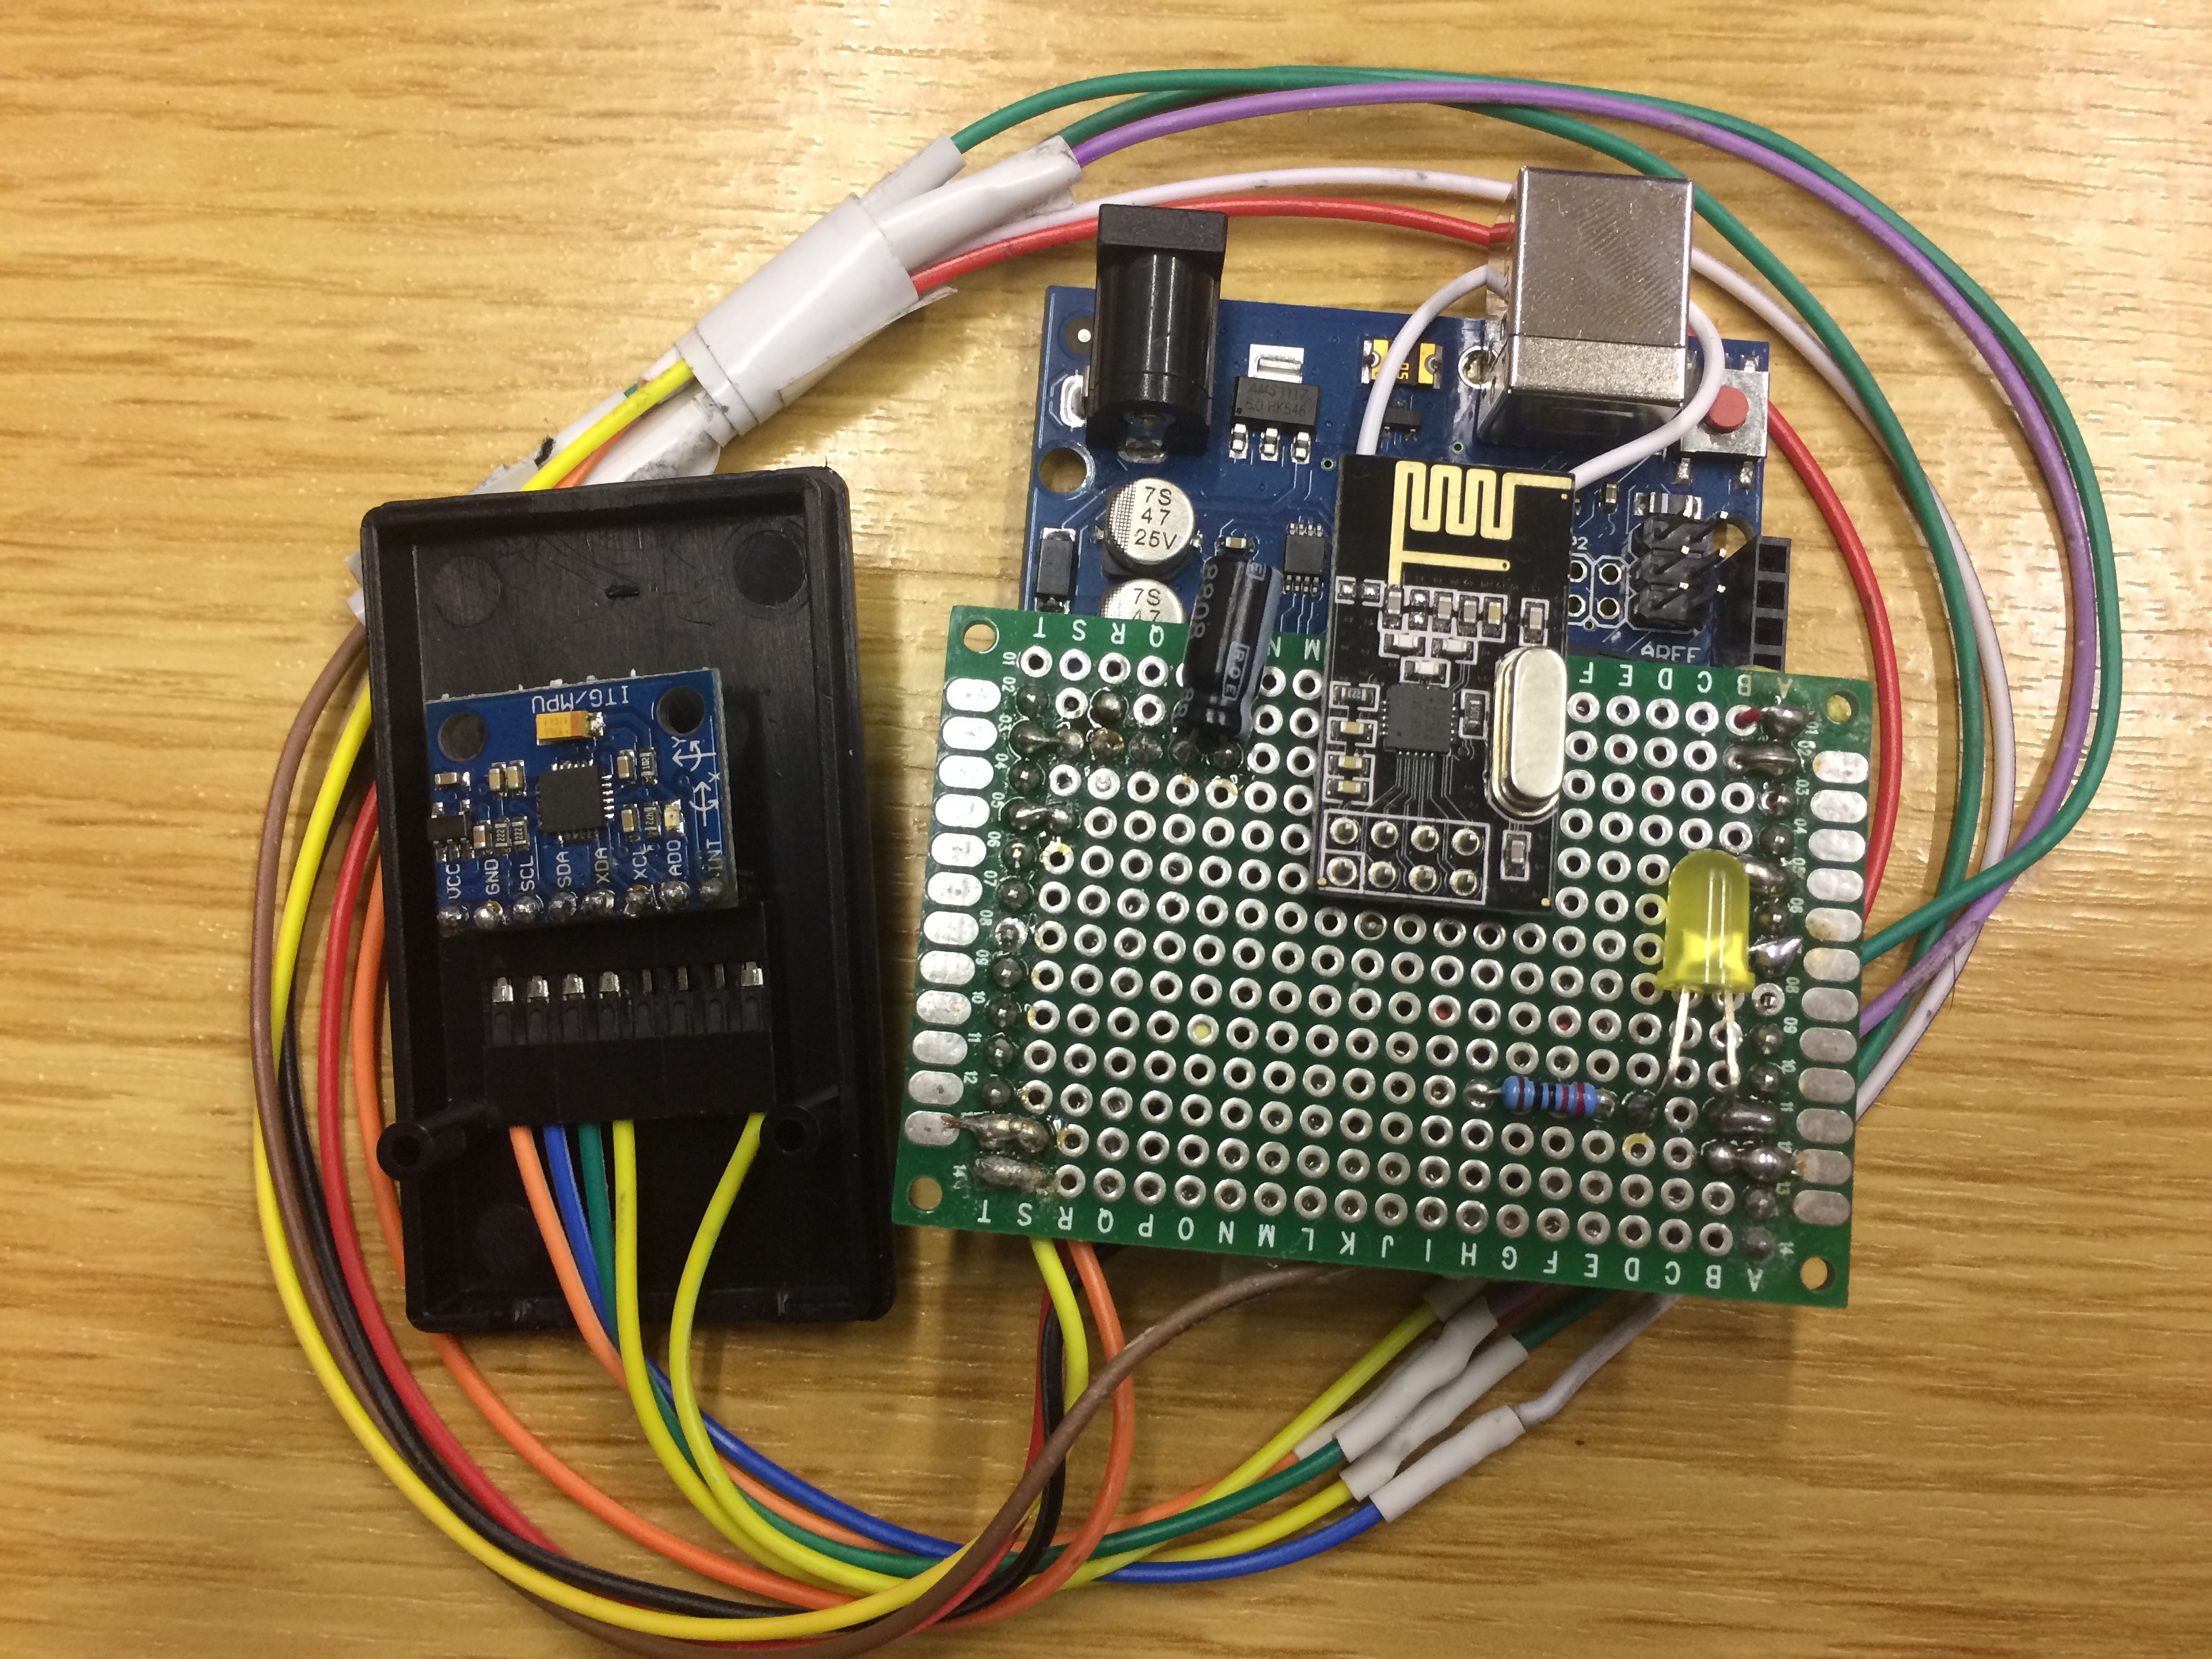
\includegraphics[width=5cm,height=3cm]{images/04-activity/sender.jpg}
	    \caption{}
	  \end{subfigure}
	  ~
	  \begin{subfigure}[t]{0.5\textwidth}
      	\centering
	    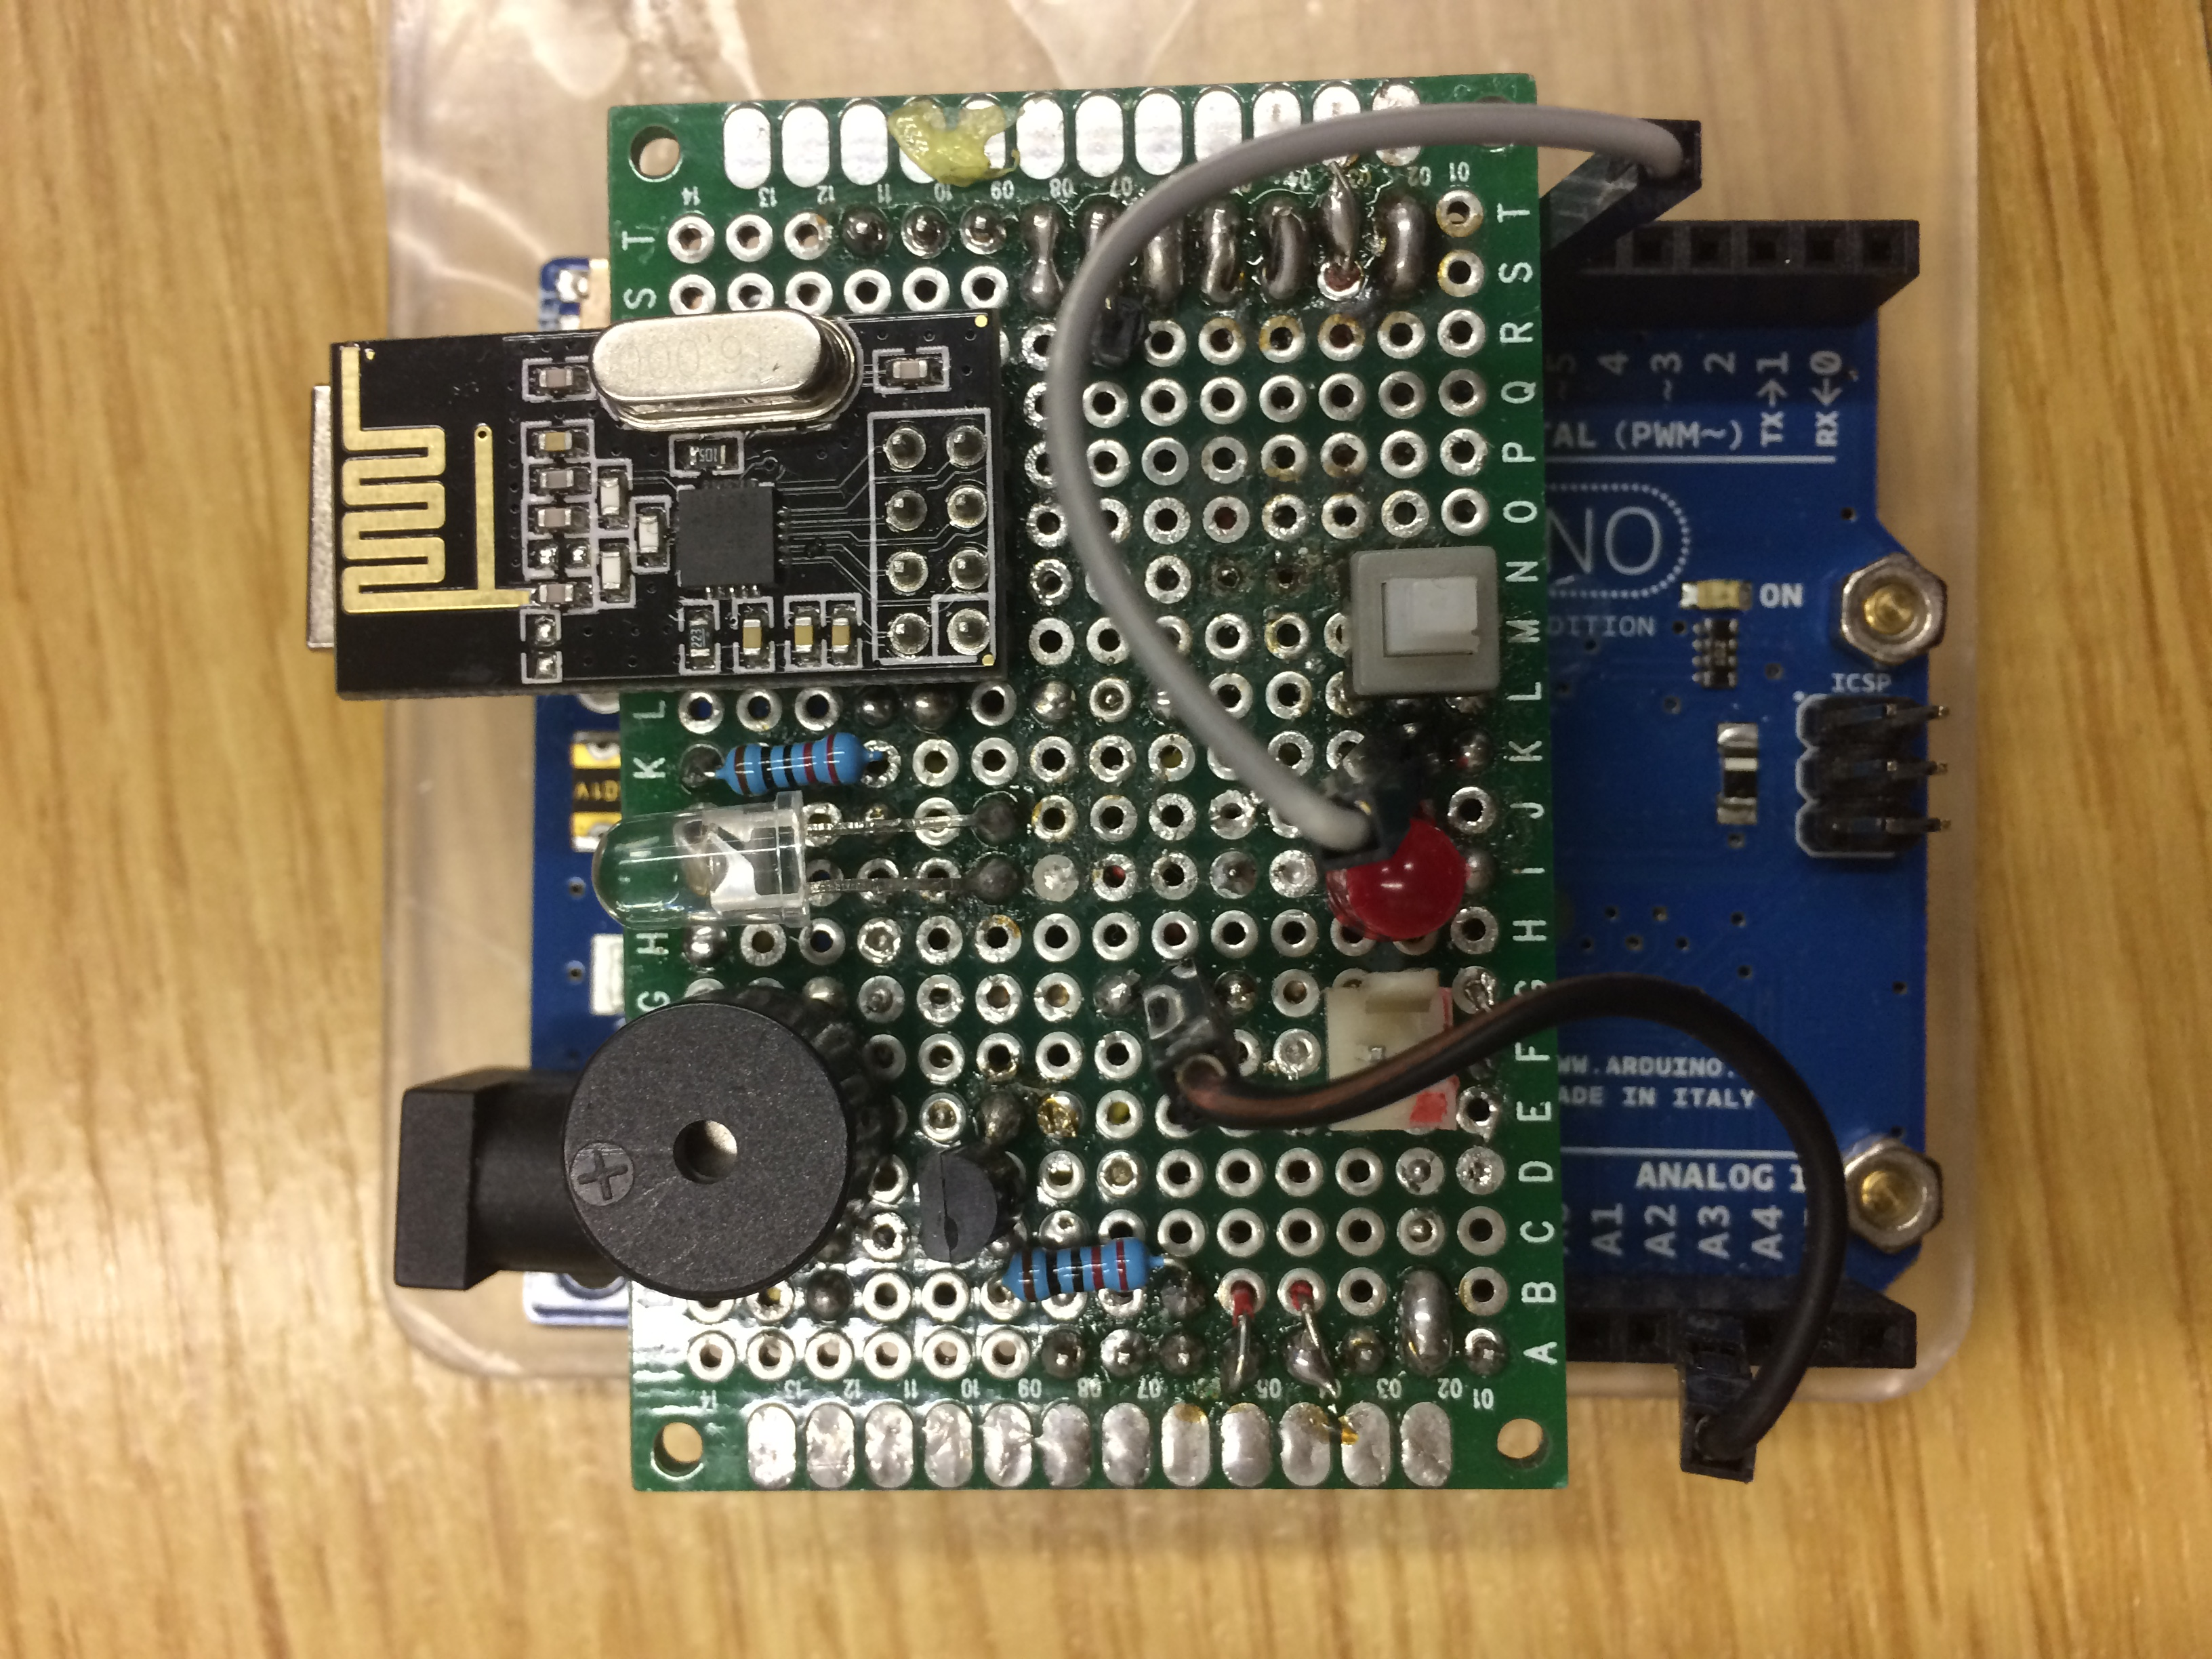
\includegraphics[width=5cm,height=3cm]{images/04-activity/receiver.jpg}
	    \caption{}
	  \end{subfigure}
      \caption{a) the accelerometer transmitter circuit and b) the receiver circuit used onboard. Both circuit are based on Arduino boards.}\label{fig:the_accelerometer}
\end{figure}

The choice of the accelerometer position was conditioned by the need to minimize the influence of noise due to irrelevant player motion.

\begin{figure}[thpb]
      \centering
      {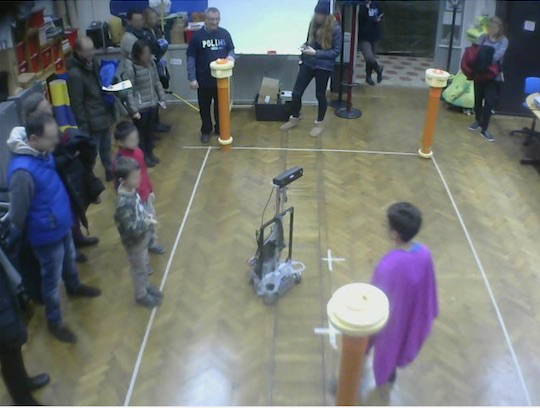
\includegraphics[width=8cm]{images/04-activity/event.jpg}}
      \caption{Human player (in magenta) during the game. The playground configuration in this trial consisted of 3 target towers.}
      \label{game}
\end{figure}

For example, hand-waving when pressing buttons are not supposed to be meaningful to identify player activities, since the full state of towers is transmitted to the robot via wireless communication including the fact that the player is pressing the button. Therefore, having the device placed on the wrist, or other highly movable body-part (as the feet or head) would capture useless acceleration information contributing to a worsening in classification accuracy. We decided to place the accelerometer on the chest, in order to capture the essential player motion.

In terms of collected data, for this work, we considered 29 matches involving 15 male participants of different ages. The age distribution consisted of children (7-10) and adults (26-40). Matches had a minimum time duration of about 40 seconds and a maximum of about 1 minute and 10 seconds. 

The collected data correspond to acceleration values along x, y, and z axis with a sampling frequency of 50Hz, which is five times higher than the frequency considered to be sufficient for detecting daily activities from accelerometer data (10Hz)~\citep{atallah_sensor_2010, ravi_activity_2005, kikhia_analyzing_2014}.

\begin{figure*}[!t]
\normalsize
      \centering
      {\includegraphics[width=\textwidth, height=4cm]{images/04-activity/diagram.png}}
      \caption{Overview of the activity recognition system.}
      \label{approach}
\end{figure*}
  
\subsection{Activity analysis}\label{sec:activity_analysis}

In our game, by using an accelerometer attached to the player, we were mainly interested on identifying activities that would help to describe the player interaction level. For the scope of this work, we aimed at identifying recurrent physical activities that would be useful for achieving that goal. From the collected data, we were able to identify a few high-level activity types, listed below:

\begin{itemize}
\item  \textbf{running:} describes a running activity. For this experiment, multiple styles of running are not considered. For instance, ``fast'' or ``slow'' running are considered as the same.
\item \textbf{walking/dodging:} represents the walking and dodging activity. The latter refers to a sudden quick movement to avoid the robot or to call its attention.
\item  \textbf{locally\_moving:} a player generic motion that is too small to fall into other categories, but not so small to be characterized as inactivity. Motion to block to block the path of the robot also fall into this type of motion.
\item  \textbf{inactive:} motion that are too low in intensity to be characterized as one of the above activities. A crisp threshold is used to delimit this category. 
\end{itemize}

By analyzing the data, we observed that player activities occur in ``bursts'' that are followed by a short period of inactivity (or rest), i.e., a short period where the player is not really moving, or the expressed acceleration is too small to be related to any activity of interest.

Resting periods are a common characteristic present in any physical game and is related to the organic human need for resting after an intense physical activity or even during strategic moments of pause. Examples of this can be seen when the player is pushing a button on a tower, or is trying to block the robot's path or even when is waiting still for a specific robot position on the environment.

On such moments of inactivity, the changes in acceleration are usually small, reflected in a relative flatness of the signal (e.g., secs 9-12 and 15-18 on Figure~\ref{acc_graph}) and this enables the delimitation of an activity begin/end moment.

\begin{figure}[h]
      \centering
      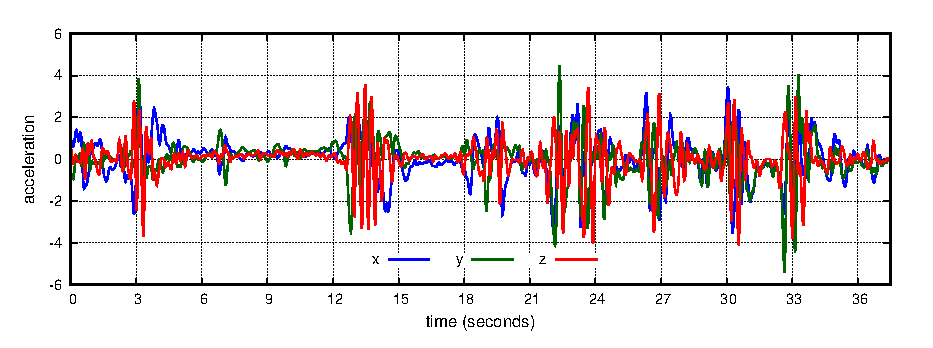
\includegraphics[width=\linewidth]{images/04-activity/newGraph.eps}
      \caption{Graph of acceleration in x, y and z axis for a game that lasted about 40 seconds.}
      \label{acc_graph}
\end{figure}

One way to describe the activity information associated to the acceleration patterns is by considering the amount of signal ``turbulence''. As a measure of such turbulence, we rely on the information present on the signal variance. 

For this, we processed the incoming data stream by computing the standard deviation of the signal inside a sliding window. This transforms the original input space in a new space where activity information is much more evident, resulting in the generation of a continuous graph, where pulses refer to a given player's physical activity (see Figure~\ref{fig:std_graph}).

Working in this way turns out to be simpler than to perform data annotation by, for instance, using a predefined sliding windows size. In our case, activities, such as ``running'', do not have fixed time duration, which makes the applicability of fixed sliding windows methods not quite suitable~\cite{noor_adaptive_2016}.

\begin{figure}[H]
      \centering
      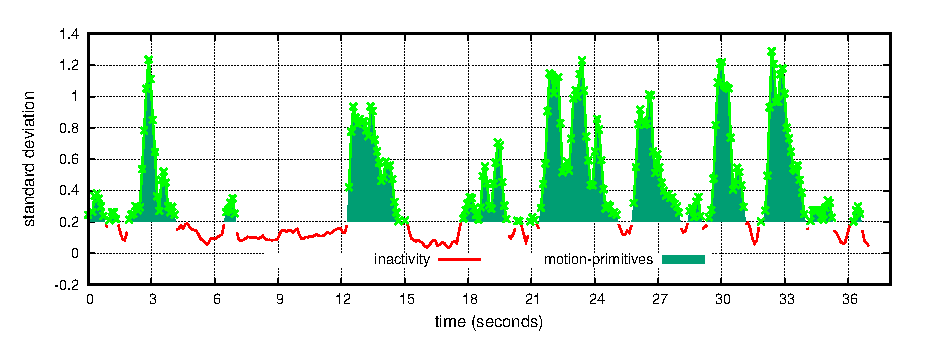
\includegraphics[width=\linewidth]{images/04-activity/newStdGraph.eps}
      \caption{Standard deviation of the acceleration in Figure~\ref{acc_graph}, computed using a sliding window of half a second. The red line portions represent variance values inside the inactivity zone (below a threshold of 0.2). Green areas are referenced as ``motion primitives''.}\label{fig:std_graph}
\end{figure}

After performing the mentioned data transformation, we have empirically identified a crisp threshold that would catch irrelevant signal values, thus, we say that any value below that threshold is related to player's inactivity.

The inactivity threshold is game-dependent and sensitive to the position of the accelerometer as well. On our experiments, the selection of the inactivity threshold is done manually, via inspection of video recorded during the game.

\begin{figure}[H]
    \centering
    \begin{subfigure}[b]{0.3\textwidth}
     	\centering
        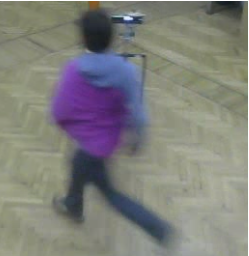
\includegraphics[width=3cm,height=3cm]{images/04-activity/enricorun.png}
        \caption{}
	\end{subfigure}
	~
    \begin{subfigure}[b]{0.3\textwidth}
     	\centering
        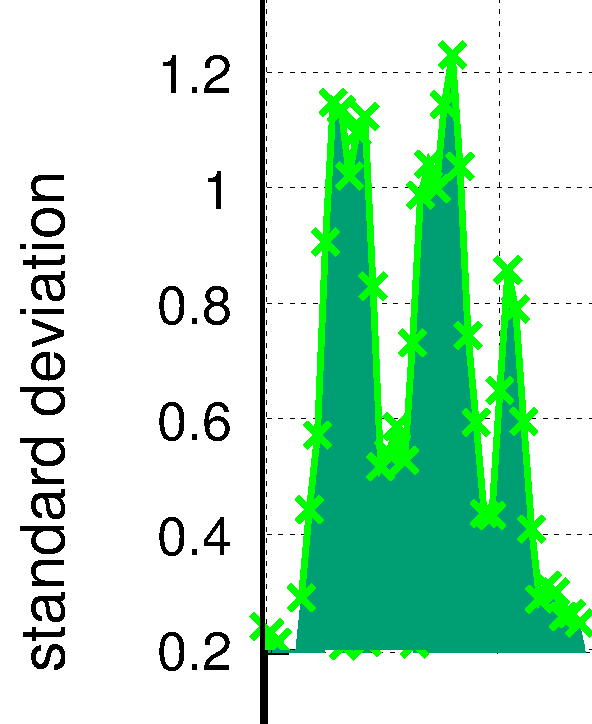
\includegraphics[width=3cm,height=3cm]{images/04-activity/run1.png}
        \caption{}
	\end{subfigure}
	\caption{a) Player performing a running activity;  b) Associated running motion primitive.}\label{fig:running}
\end{figure}

\begin{figure}[H]
  \centering
  \begin{subfigure}[b]{0.3\textwidth}
  	 \centering
      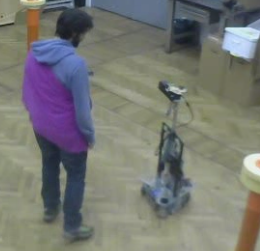
\includegraphics[width=3cm,height=3cm]{images/04-activity/enricostill.png}
      \caption{}
  \end{subfigure}
  \begin{subfigure}[b]{0.3\textwidth}
  	 \centering
      
\includegraphics[width=3cm,height=3cm]{images/04-activity/still.png}
      \caption{}
  \end{subfigure}
  \caption{a) Player performing local movements; b) Associated motion primitive.}    
  \label{fig:localmov}
\end{figure}
    
Since any motion information below the threshold is used to determine the ``inactivity'' of the player, we use machine learning-based classification only on each data interval above the threshold. This interval is called a ``motion primitive'' (Figure~\ref{fig:std_graph}). The motion primitives are the data aggregations to which we associate a class label in the annotation procedure. 

Following the classification need, we have extracted the following descriptors from the motion primitives (recall: they refer to standard deviation of the raw values): 

\begin{itemize}
\item \textbf{mean}:  the mean values.
\item \textbf{activity\_time}: the time duration in seconds.
\item \textbf{max\_peaks}:  the max peak.
\item \textbf{number\_of\_peaks}:  the number of peaks.
\item \textbf{mean\_of\_peaks}: the mean of all peaks.
\item \textbf{max-min}: difference between max and min.
\item \textbf{std}: standard deviation.
\item \textbf{mad}: median absolute deviation.
\item \textbf{sma}: signal magnitude area.
\item \textbf{energy}: the signal energy.
\item \textbf{iqr}: interquartile range.
\item \textbf{mean\_over\_max}: mean of peaks divided by the max peak.
\item \textbf{maxInd}: index of the frequency component with largest magnitude.
\item \textbf{meanFreq}:  weighted average of the frequency components to obtain a mean frequency.
\item \textbf{skewness}:  skewness of the motion primitive.
\item \textbf{kurtosis}:  kurtosis of the motion primitive.
\item \textbf{freq-skewness}: skewness of the frequency domain signal.
\item \textbf{freq-kurtosis}: kurtosis of the frequency domain signal.
\item \textbf{pse}: Power spectral entropy.
\item \textbf{rms}: Return the root mean square.
\end{itemize}

\begin{figure}[htbp]
     \centering
     {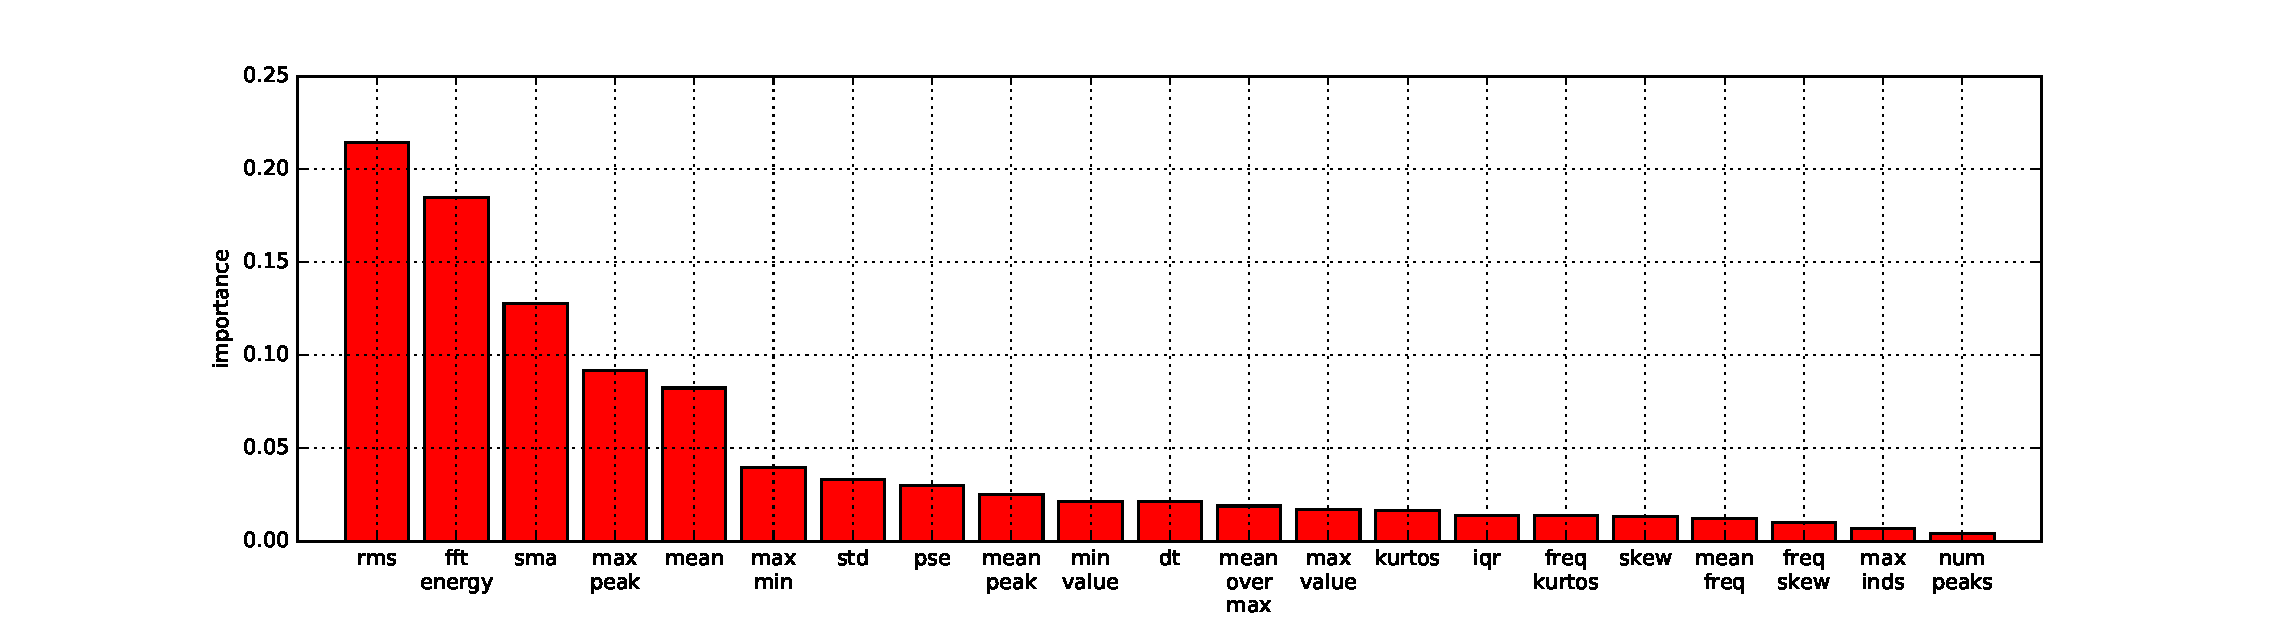
\includegraphics[width=\textwidth]{images/04-activity/featureImportance}}
     \caption{Feature importance computed by a forest of decision trees classifiers.}
     \label{fig:feature_importance}
\end{figure}

Note that the motion primitives carry sufficient information to distinguish between target physical activities. For example, ``running'' is related to a motion primitive that has a longer duration and a higher amplitude value (see Figure~\ref{fig:running}) as opposed to the duration and amplitude values of a player local motion (figure~\ref{fig:localmov}). Following the same argument, a ``walking'' activity has higher amplitude values compared with a local movement. A holistic view of the classification approach is detailed in Figure~\ref{approach}. 

\subsection{Classification setup}

For the automatic classification, we first build the standard deviation graph from the raw accelerometer data, and then we manually label motion primitives. 

On our experiments, the std graph was generated considering a sliding window 500msec long with no overlap, resulting on a dataset composed by $367$ motion primitives. Empirically, this time length turned out to be descriptive enough to produce variance intervals that made it possible to distinguish activities. Naturally, the windows size has an impact on the total number of motion primitives generated per game match, as well as on the inactive threshold value. With a windows size of half a second, however, it was possible to capture immediate transition between activities, given that such transition would manifest on higher spikes on variance at the beginning of an activity. For this reason, we kept the mentioned size. 

The primitives were labeled as follows: $34\%$ as ``locally\_moving''; $25\%$ as ``walking/dodging'' and $41\%$ as ``running''. The remaining percentile was left out due to the incapacity in identifying a underlying activity (maybe because the player was moving too slow or aimlessly) or because the data explicitly did not corresponded to one perform when playing. As argued above, the ``inactive'' type had not to be labeled, since it is directly classified by the inactive threshold. From video log inspection, we observed that most of the useless motion would occur below a threshold of $0.2$.

Before training classifiers, we performed feature selection by evaluating the importance of the extracted features (see section~\ref{sec:activity_analysis}) using random forest method, composed by 300 decision trees. (see Figure~\ref{fig:feature_importance}).

\section{Results and discussion}\label{sec:activity_discussion}

We tested different classifiers using 10-fold cross validation in order to have a more descriptive accuracy information. Following common practice, the train-test dataset ratio was defined as 80\% and 20\% respectively.

\begin{table}[h]\footnotesize
  \centering
  \caption{Cross-validation accuracy results for several classification methods using the 5 most significant features shown in Figure~\ref{fig:feature_importance}.
  }
  \begin{tabular}{| c | c |}
    \hline
  	   \textbf{Method}          & \textbf{Accuracy}\\\hline
       SVM (Linear Kernel)      & 0.80 (+/- 0.08)  \\\hline
       Random Forest            & 0.81 (+/- 0.06)  \\\hline
       Gaussian Naive Bayes     & 0.80 (+/- 0.11)  \\\hline
       Ensemble (Hard voting)   & 0.82 (+/- 0.10)  \\\hline
       AdaBoost                 & 0.65 (+/- 0.40)   \\\hline
  \end{tabular}
  \label{accuracy5best}
\end{table}


Table~\ref{accuracy5best} presents 10-fold cross validation results using different classifiers on the five most important features, that is: \textit{rms}, \textit{fft\_energy}, \textit{sma}, \textit{max\_peak} and \textit{mean}. 

The ensemble reported in Table~\ref{accuracy5best} is defined as a majority (Hard) voting approach by the combination of the SVM, Gaussian Naive Bayes and Random Forest. The Adaboost method, in turn, takes a combination of 100 weak classifiers (Decision Trees). All methods were trained by using Python Scikit-learn machine learning library.

Despite the effort, with a confidence interval of 95\% we see that SVM, Random Forest, Gaussian Naive Bayes as well as their ensemble have a similar accuracy result. By considering the variance in their result, we see that Random Forest gives the most stable result. 

\begin{table}[h]\footnotesize
  \centering
  \caption{Classification report for the chosen ensemble method (Random Forest). F1-score is the classical metric for binary classification evaluation. LM, WD and R stands for \textit{Locally Moving}, \textit{Walking/Dodging} and \textit{Running}, respectively.
  }
  \begin{tabular}{| c | c | c | c | c |}
    \hline
  	   & precision   & recall & f1-score &  support \\\hline
    LM &      0.88   &  0.91  &    0.89  &      23  \\\hline
    WD &      0.79   &  0.60 &     0.68 &       25  \\\hline
     R &      0.77   &  0.92 &     0.84 &       26  \\\hline
avg/total &   0.81   &  0.81 &     0.80 &       74  \\\hline
  \end{tabular}
  \label{report}
\end{table}

Given the 10-fold cross validation results, we decided to use as final method the Random Forest ensemble classifier (10 decision trees). Detailed results for the method are shown in table~\ref{report} and the corresponding confusion matrix and~\gls{roc} in Figure~\ref{fig:mtx-roc}. The majority of mistakes in the classification correspond to the difficulty in separating ``walking/dodging'' from  a ``running'' activity. 

The justification for this may be on the fact that occasionally the player walks in a fast way, which is similar to proper running. This is acceptable given that even for humans it is not straightforward to decide about the boundary conditions of two different, but related activities.

Despite the fact that our method relies on the computation of a fixed sliding window when transforming the input data, we see that our method also allows for a small improvement in the annotation procedure. Consider, for example, that we do not have to worry about the effects of overlapping windows. Things like the choice of windowing functions, which are used to mitigate the effects of overlap, are not needed. Also, it allows for a more intuitive way of perceiving what underlying activity has occurred.

We have conducted experiments on using our method online, and the results have been satisfactory. One drawback, however, is on the possibility of having two different activities associated to the same motion primitive. This is likely to occur when the player rapidly shifts between two activities. For example, this happens when the player stops running for a fraction of a second and then immediately starts walking. In that case we see a small decrease in the signal variance that may not be enough to characterize an inactivity period. Note that a value below the inactive threshold is the event that separates motion primitives.

\begin{figure}[h]
    \centering
    \begin{subfigure}[h]{7cm}
       \centering
       \includegraphics[width=7cm, height=5cm]{images/04-activity/conf_mtx.eps}
       \caption{}
	\end{subfigure}
	~
    \begin{subfigure}[h]{7cm}
     	\centering
        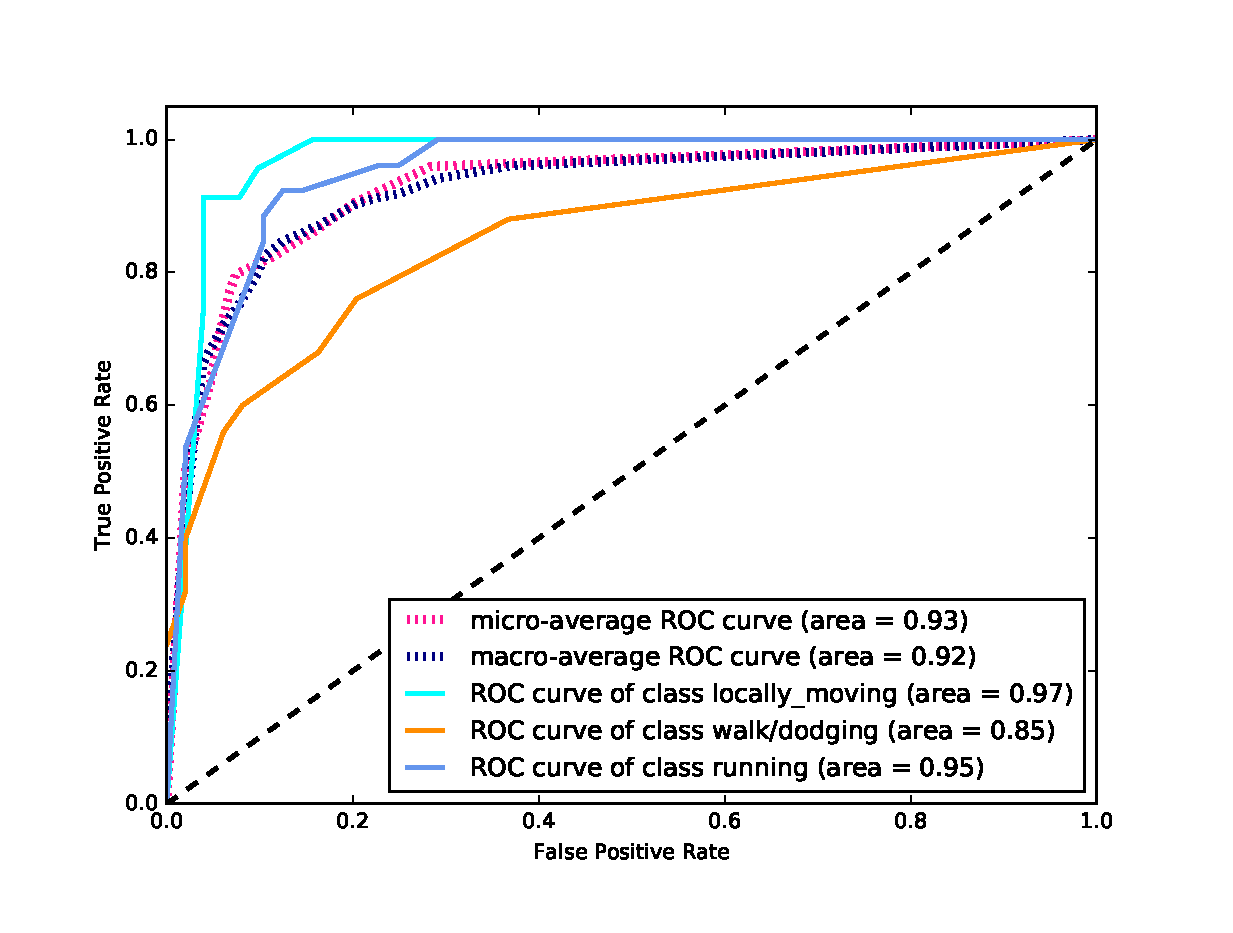
\includegraphics[width=7cm, height=6cm]{images/04-activity/roc.eps}
        \caption{}
	\end{subfigure}
	\caption{a) Confusion matrix for the trained Random Forest ensemble method and the associated. b) \gls{roc} curve.}\label{fig:mtx-roc}
\end{figure}

\section{Considerations}

In this activity recognition work, we have investigated the recognition of high-level human player activity in our~\gls{pirg} scenario. We have used the variance in player acceleration as data instances and primary source of information from where to extract features and then train a~\gls{ml} model. The devised system can be used as base to model the overall player behavior by differentiating activity frequencies among the different players. This model can than be used to guide the agent in the adaption of its strategies to support the player entertainment. Following this goal, in the next chapter we present some insights for player models, building up from the activity system presented in this chapter.

In chapter~\ref{ch:modeling} we will present some ideas on modeling player activity by features extracted from their spatial relationship with the robot as estimated from laser data

This type of data is more reliable compared to those from the accelerometer. Additionally, the use of lasers removes the concerns related to the introduction of noise from eventual misplacement of the accelerometer on the player's chest. Since the accelerometer had to be placed on each new player, eventual misplacements may modify the distribution of data used for training (input space) the algorithm, resulting in loss of accuracy. 

\chapter{Player behavior modeling}\label{ch:modeling}

Having identified an activity recognition system, we aimed at the definition of an approach to model user behavior that could account for the combination of the player physical effort and interaction level. The proposed model is based on the human activity recognition (chapter~\ref{ch:activity}) and a description of interaction (proximity and body contraction index) relative to the robot co-player.

\section{Relational Activity Model}\label{sec:simple_model}

As in~\cite{etheredge_generic_2013}, we defined as behavior a sequence of discrete time-bounded actions performed by the player. Since we are dealing with a physically interactive scenario, these time-bounded actions have strong relation with the amount of physical activity spent, hereby considered as the human ``activity effort''. The relationship with the robot, on the other hand, is considered as the ``relative interaction''. 

In the proposed model, the two dimensions (activity and interaction) are combined into a simple overall scoring system capable of describing quantitatively the player's active participation in the~\gls{pirg}. The proposed model is detailed in the next.

\subsection{Activity}\label{activity}

Equation~\ref{eq:activity_eq} is used to compute the general amount of activity $\alpha(m)$, given the classification of primitive motions from chapter~\ref{ch:activity}:

\begin{equation}
	\alpha(m)=\sum_{i \in \mathcal{A}} \omega_{i}\varphi_i(m);\qquad m \in \mathcal{M}
	\label{eq:activity_eq}
\end{equation}
, where $\mathcal{A}$ stands for the set of activities \{``running'', ``locally moving'', ``walking/dodging''\}; $\omega$ stands for the activity weight; $\varphi$ for the stochastic prediction value for the motion primitive $m$.

We consider equation~\ref{eq:activity_eq} as a measure of the ``effort'' of the player. The weight $\omega$ states how much each physical activity contributes to the overall quantification and is a hyper-parameter intended to capture the partial ordering among activities.

\subsection{Interaction}\label{Interaction}
In order to model the interaction we take into account the spatial relationship between the player and the robot defined as \textit{proximity} and a measure of body contraction named~\gls{ci}.

Proximity is a measure defined in the interval [0, 1], computed from the data provided by Microsoft Kinect\textsuperscript{\textregistered}, normalized according to the sensor specifications (see section~\ref{sec:kinectsec}).~\gls{ci} is also in [0, 1] and it is calculated using a technique related to the bounding region, i.e., the minimum rectangle surrounding the body: the algorithm compares the area covered by this rectangle with the area currently covered by the player's silhouette~\citep{castellano_recognising_2007}.


%EWERTON: I have red
%ISSUE: Not providing data and analysis to support this makes this assumption quite weak.
    %PROBLEMATIC PARAGRAPH: A high~\gls{ci} is associated with an intense interaction because a wide openness of the body is interpreted as a higher focus level of the player w.r.t the robot and the game; for this reason it will boost the final outcome. Low~\gls{ci}, in turn, is interpreted as a lack of focus or, in general, limited motivation of the player, which penalizes the interaction.
% REWRITTEN: (BELOW)
The~\glsdesc{ci} can be viewed as a measure of focus and in our application it tries to capture, via body contraction, the amount of attention in the robot movement. It is so because~\glsdesc{ci} can be seen as correlated with situations demanding high attention in other physical games. For example, highly concentrated players in a soccer game tend to keep their arms opened when dealing with a situation demanding high attention, like and attack or penalty. To us,~\gls{ci} tends to be high when players are expecting a response by the robot and tends to be low when situations are not risky. Figure~\ref{fig:low_high_CI} depicts two situations where the~\gls{ci} is different and show different level of attention.

\begin{figure}[h]
    \centering 
	\begin{subfigure}[h]{0.48\textwidth}
		\centering      
		\framebox{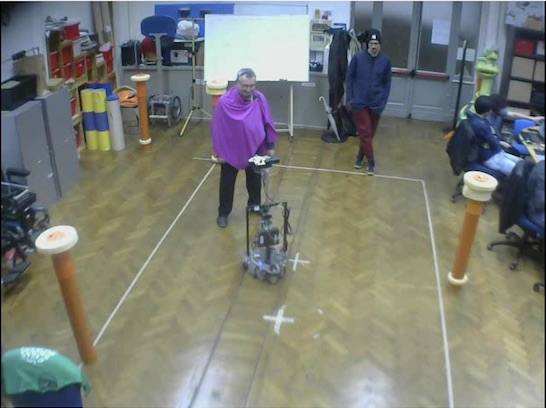
\includegraphics[width=5cm]{images/07-modeling/lowCI.jpg}}
		\caption{}
	\end{subfigure}
	~
	\begin{subfigure}[h]{0.48\textwidth}
		\centering      
      	\framebox{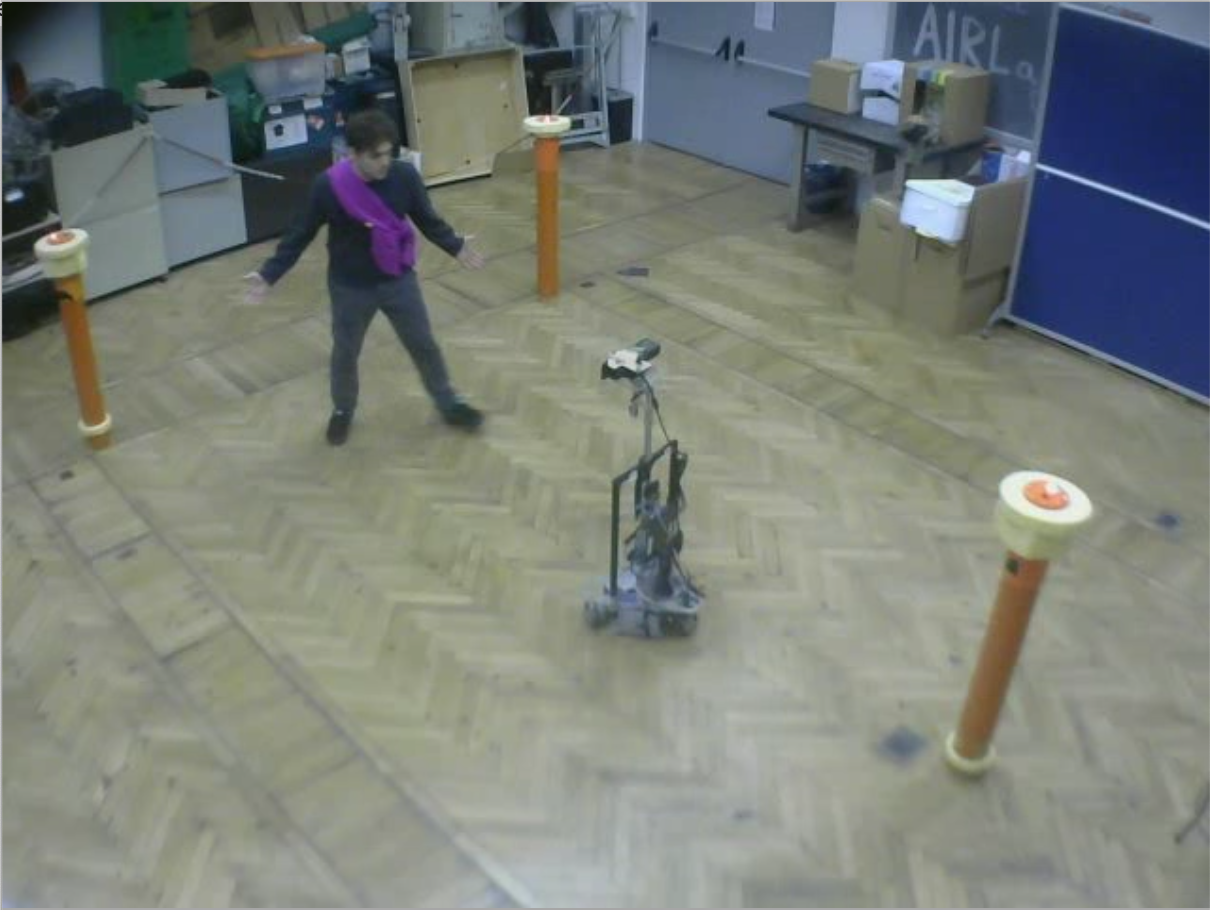
\includegraphics[width=5cm]{images/07-modeling/highCI.png}}
      	\caption{}
     \end{subfigure}
      \caption{Example of situations with different CI values. a) Situation with low CI were the player has a more contracted body. b) Situation with a higher~\gls{ci} compared to the situation in the left. Here the player has a larger body aperture.}
      \label{fig:low_high_CI}
\end{figure}

\subsection{Combined model}\label{sec:engagement}
The model to describe the player relational activity is a combination of the activity level and the degree of interaction, named $\epsilon$; it summarizes the player physical activity during the game and has a linear relationship with his interaction with the robotic opponent as follows: 
\begin{equation}
\label{enagementeq}
\epsilon=\rho\alpha(m),
\end{equation}
, where $\rho$ is the estimated amount of interaction between the players. The variable $\epsilon$ is a simple linear relation that puts in relation interaction and physical activity. Here $\rho$ is an overall degree of interaction, i.e., the combination of~\gls{ci} and proximity and should not be zero. The combination of the interaction signals is not bound to a specific method. In this work, we have used a fuzzy logic system to obtain the desired combination, described in a linguistic way. In principle, the combination of the signals depends on the specifics of the~\gls{pirg} environment.

For the evaluation of the model we have reused the same data from section~\ref{sec:data_collection}. The model output for two different players can be seen in Figure~\ref{fig:model_output}. In Figure~\ref{fig:fun}, the player is perceived as more active than the one in fig.~\ref{fig:nofun}, which is reflected by the difference in the inactivity time and the amplitude of the bars.

\begin{figure}[h]
    \centering 
	\begin{subfigure}[h]{5cm}
		\centering      
		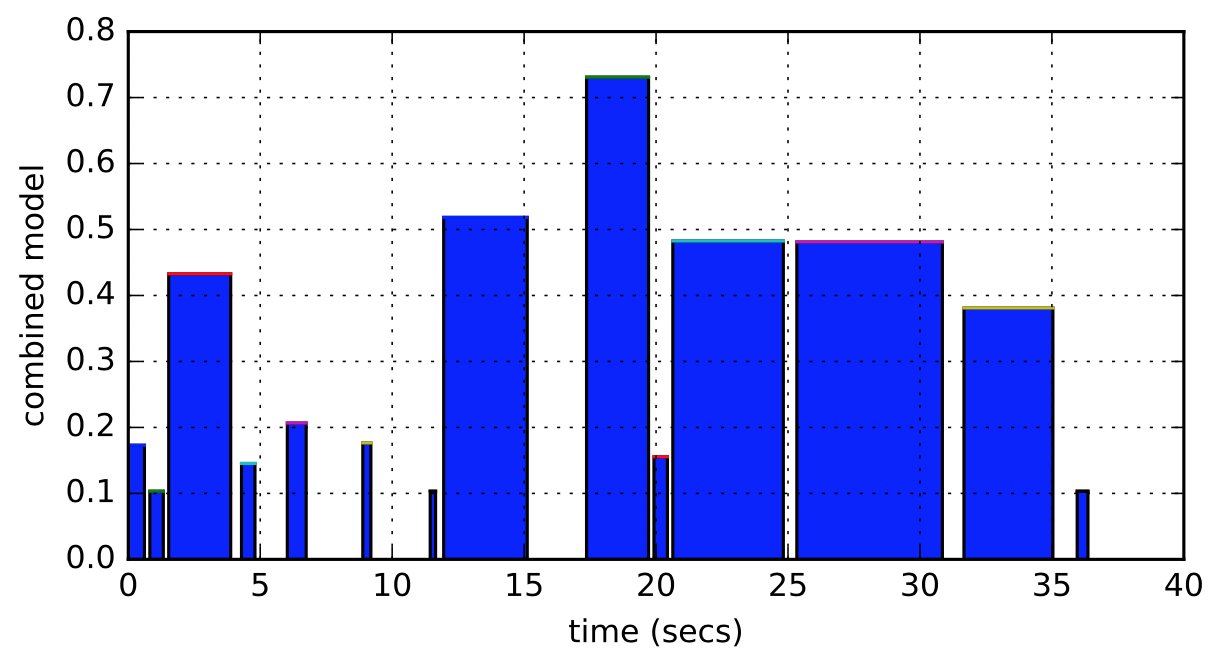
\includegraphics[width=5cm]{images/04-activity/combined.png}
		\caption{}
		\label{fig:fun}
	\end{subfigure}
	~
	\begin{subfigure}[h]{5cm}
		\centering      
      	\includegraphics[width=5cm]{images/04-activity/combined_less.png}
      	\caption{}
      	\label{fig:nofun}
     \end{subfigure}
      \caption{a) Model results for a single match that lasted 45 secs. b) Model output for a less active player. The plot refers to 30 initial secs of activity.}		
      \label{fig:model_output}
\end{figure}

The model quantitatively describes, in a simple way, the player's relational activity by the combination of the amount of physical activity and interaction relative to the robot. This can be used as a metric expected to enable the robot to take into account the player's attitude in order to adapt its own activity to match it. Using this model, for instance, an active player could be viewed as one having a larger cumulative sum of $\epsilon$ values up to a point in time.

However, this model is limited in several ways, %TODO I cannot evaluate it since I cannot understand it
one of which is the manual definition of weights for the activities ($\omega$). Manually selecting these scaling factors becomes difficult as the number of activities grows. With this in mind, we have then worked on a definition of a more robust player model relying on latent representation which is described in the next section.

\section{Latent player modeling}

We attempted to improve the previous model in several ways. First, by mapping the stream of accelerometer data to an image representation, called Gramian Angular Field (GAF) images~\citep{wang_imaging_2015}, in order to take advantage from algorithms for unsupervised feature extraction, such as autoencoders~\citep{goodfellow_deep_2016}, and reduce the effort of handcrafting representation features for the user behavior. After the definition of a dictionary of primitives on the feature space, we apply ~\gls{lda}~\citep{blei_latent_2003}, a discrete generative model (an admixture model) mostly used for document retrieval and classification, to uncover coherent groups of motion patterns that can be used to categorize players.

The model here is comprehensively different from the simple one presented in the previous section: it does not take into account features of interaction, but only the player's acceleration patterns (despite not being considered in literature, there is no fundamental constraint that prevents the use of such data). There is also no need to manually set scaling factors from target activities since the model explores the importance of each acceleration spike by itself. Furthermore, the model is able to provide the distinction between players so that it can be easily used for clustering. Each player is represented by a normalized vector where each component denotes the proportion of membership to a given class of players obtained from data.

In particular, our decision to use~\gls{lda} was inspired by the work of~\cite{smith_mining_2016}, which considers each game session as a ``document'' and the player generated data stream as the ``words'' of such document. The interpretation of game session as documents and player data as words preserves the jargon of the text mining and information retrieval literature from which~\gls{lda} is most used for. The main assumption is that different players generate different streams of input words, thus different ``documents'', depending on their own motivation or play style. 

The feasibility of applying~\gls{lda} to this problem is further reinforced by noticing the apparent difficulty in objectively separating the existing types of motion patterns in the acceleration signal via inspection. A player in his/her playing activity may show different motion patterns that are often not clearly distinguishable from each other and thus not easy to provide a supervision for,~\ie a class tag. Here, the assumption is that a high motion profile, i.e., high turbulence in acceleration signal, is typical for a highly motivated player, since we believe a non-motivated player tends to stay relatively still, or to show a very low acceleration profile.

The claim that motion patterns convey engagement or even emotional state~\citep{aristidou_emotion_2015,shafir_emotion_2016,tsachor_somatic_2017} has been supported by several academic papers. Systematic approaches for describing body movement, such as~\gls{lma}~\citep{laban_language_1974} are used to derive low-dimensional representation of mood, facilitating affective motion modeling~\citep{burton_laban_2016}. This same type of analysis has been applied when investigating motor elements that characterize movements whose execution enhances basic emotions, such as: anger, fear, happiness and sadness~\citep{shafir_emotion_2016}. In game situations, despite the limited capacity for entertainment detection and modeling in Exergames, \gls{lma} had been reported as useful in fostering emotion recognition in states like: concentration, meditation, excitement and frustration~\citep{zacharatos_emotion_2013}.

Here, we hypothesize that, on average, a player will display his/her game-intrinsic motion style and convey some information about his/her interest in playing. Discovering which coherent groups of motion style exist in a dataset makes it possible to estimate to what extent an unknown player relates to known groups in terms of his/her own motion profile. This may ultimately support the design of~\gls{pirg}s able to adapt in order to offer a better play experience.

In summary, in our methodology a player is represented by how much of each discovered motion groups (called motion \textit{topics}) his/her data is likely to be generated from. Such representation is called the player's \textit{mixture proportion} of motion types and is akin to the mixture proportion of documents in topic modeling applications~\citep{blei_latent_2003}. We expect to see similar players grouped together in a coherent collection, enabling to distinguish among them and their motion types. The results obtained using the dataset detailed in section~\ref{sec:data_collection} are validated with human supervision, suggesting the applicability of our method to future mechanisms for designing auto-adapting agents.

\subsection{Problem Statement}
This section formulates the problem of modeling the player as a probabilistic mixture of player styles derived from data. One can see that it is a step towards advancements in the dimension of design referred to the ability to play for engagement maximization, as discussed in section~\ref{sec:dimensions}.

Here, we use data coming from a single accelerometer placed on the human player's body as in Chapter~\ref{ch:activity}. For the current study, player movement is our primary source of information for characterizing the playing style. The basic assumption is that a highly active player would naturally express his/her status by a very turbulent motion signal, making the signal compatible with strong in-game activity. Consider, for instance, the difference in signal shapes reported in Figure~\ref{figure:acc_signal_shape}.

\begin{figure}[h]
    \centering
    \begin{subfigure}[h]{\textwidth}
        \centering
        \includegraphics[width=0.2\textwidth]{images/05-modeling/enricorun} 
        \includegraphics[width=0.6\textwidth]{images/05-modeling/running_sig_profile} 
        \caption{}
    \end{subfigure}\vspace{6pt}
    ~
    \begin{subfigure}[h]{\textwidth}
        \centering
        \includegraphics[width=0.2\textwidth]{images/05-modeling/enricostill}
        \includegraphics[width=0.6\textwidth]{images/05-modeling/standing_sig_profile} 
        \caption{}
    \end{subfigure} \vspace{-6pt}
    \caption{Three-axis accelerometer signal during game play. a) A running player. b) A player standing still. Signal shape and amplitude are very characteristic for the respective activity.}
    \label{figure:acc_signal_shape}
\end{figure} \unskip

In other words, following this line of reasoning, we also assume players do not fake their engagement by unnecessarily performing strong activities, like running, when they are actually not engaged in the game or feel bored by the robot behavior. Therefore, we assume that a highly motivated player would act more intensively and frequently than a non-motivated one, thus showing a more turbulent acceleration signal profile. In situations like~\gls{pirg}, movement information is useful and should not be disregarded. Furthermore, a model that is able to extract a description of the player's movement profile for the purpose of robot behavior adaptation would generate interesting insights on the capability of the application to engage humans.

\subsection{Mathematical background}
This section presents the basic concepts and principles behind~\gls{gaf}, autoencoders and~\gls{lda}, which are important to understand our modeling procedure.

\subsubsection{\glsdesc{gaf} Images}

The results obtained in this work rely on the transformation of the acceleration time series generated by the player into images that are then processed and understood in terms of emergent patterns. The types of image we have chosen are~\gls{gasf} and~\gls{gadf}. Such images had been proposed in the field of time series classification~\citep{wang_imaging_2015}, where the authors evaluated the efficacy of representing time series in a polar coordinate system instead of the typical Cartesian coordinates. For a deep understanding of the method, we suggest reading the work of~\cite{wang_imaging_2015} where the authors did not only present the idea of~\gls{gasf}/\gls{gadf}, but also reported experimental results comparing them with other time series techniques. Here, we present an overview of the idea behind the method in order to familiarize the reader and to point out its role in our proposal.

In general, in order to obtain a~\gls{gasf}/\gls{gadf} representation for a time series $\mathcal{X}=\{x_{1}, x_{2}, ... x_{n}\}$ of size $n \in \mathbb{N}_{>0}$, rescaling is first performed in order to put the time series in the interval $[\,-1,1] \,$ or $[\,0,1]\,$. The second step is to represent the rescaled time series $\widetilde{\mathcal{X}}$ in polar coordinates, where each sample value is now mapped into the angular cosine and the time stamp information is represented as the radius. 
The formula for this step is as follows:

\begin{equation}
\begin{dcases}
  \phi = \arccos(\widetilde{x}_{i}) \quad -1 \leq \widetilde{x}_{i} \leq 1, \widetilde{x}_{i} \in \widetilde{\mathcal{X}} \\
  r = \frac{t_{i}}{N} \quad \quad t_{i} \in \mathbb{N}_{>0},
\end{dcases}
\label{equation:GAF}
\end{equation} 
where $t_{i}$ is the time stamp and $N$ plays the role of a normalizer for the span of the polar coordinate system. Some properties of this transformation are known:

\begin{itemize}[leftmargin=*,labelsep=5.8mm]
\item \textbf{{Property \#1}}: equation~(\ref{equation:GAF}) is bijective as $\cos(\phi)$ is monotonic when $\phi \in [\,0,\pi]\,$. Given a time series, the proposed map produces a unique result in the polar coordinate system together with a unique inverse map. 
\item \textbf{{Property \#2}}: as opposed to Cartesian coordinates, polar coordinates preserve absolute temporal~relations.
\item \textbf{{Property \#3}}: rescaled data in different intervals have different angular bounds. That is, $[\,0,1]\,$ corresponds to the cosine function in $[\,0,\frac{\pi}{2}]\,$, while cosine values in the interval $[\,-1,1]\,$ fall into the angular bounds $[\,0,\pi]\,$. These intervals are known to produce different information granularity in the~\gls{gaf}, especially for classification tasks~\citep{wang_imaging_2015}.
\end{itemize}

The third step in completing the transformation is to exploit the angular perspective by considering the trigonometric sum/difference between each point. This allows for the identification of the temporal correlation within different time intervals. The two types of~\gls{gaf}, namely~\gls{gasf} and~\gls{gadf}, are obtained as follows:

\begin{equation}
    \begin{aligned}
    \gls{gasf} &= [\,\cos(\phi_{i} + \phi{j}]\, \\
    	 &= \widetilde{\mathcal{X}}' \cdot \widetilde{\mathcal{X}} - \sqrt{I-\widetilde{\mathcal{X}}^2}' \cdot \sqrt{I-\widetilde{\mathcal{X}}^2}
    \end{aligned}
\end{equation}

\begin{equation}
    \begin{aligned}
    \gls{gadf} &= [\,\sin(\phi_{i} + \phi{j}]\, \\
    	 &= \sqrt{I-\widetilde{\mathcal{X}}^2}' \cdot \widetilde{\mathcal{X}} - \widetilde{\mathcal{X}}' \cdot \sqrt{I-\widetilde{\mathcal{X}}^2}\\
    \end{aligned}
\end{equation}

The symbol $I$ is the unit row vector. After translating the time series from the Cartesian to polar coordinate system, each time step in it is taken as a 1D metric space. By defining the inner product as $<x,y> = x \cdot y - \sqrt{1-x^2} \cdot \sqrt{1-y^2}$ and $<x,y> = \sqrt{1-x^2} \cdot y - x \cdot \sqrt{1-y^2}$, respectively,~\gls{gaf}s become {quasi-Gramian} matrices, since the defined $<x,y>$ do not satisfy the property of linearity in inner-product space.

According to~\cite{wang_imaging_2015}, the~\gls{gaf}s have several advantages:

\begin{itemize}[leftmargin=*,labelsep=5.8mm]
\item \textbf{{Advantage \#1}}: they provide a way to preserve temporal information. The temporal correlation is present because $G_{(i,j||i-j|=k)}$ represents the relative correlation by the superposition/difference of directions with respect to time interval $k$. The main diagonal $G_{i,i}$ is the special case when $k = 0$, which contains the original value/angular information. 
\item \textbf{{Advantage \#2:}} from the main diagonal, it is possible to reconstruct the time series back into the original Cartesian space. This is useful especially in a classification task, where we can convert the time series back to numerical Cartesian space from the high level features learned by, for instance, a deep neural network.
\end{itemize}

However, the size of the Gramian matrix $G$ is $n \times n$, for $n$ being the length of the raw time series, which may produce issues regarding memory complexity. For this issue~\cite{wang_imaging_2015} propose a solution by attempting to reduce the size of the produced~\gls{gaf} using, for instance,~\gls{paa}~\citep{keogh_scaling_2000} to smooth the time series while preserving the trends. An example of the conversion from time series to~\gls{gasf} image is shown in Figure~\ref{figure:gasf_example}.

\begin{figure} [h]
\centering
\includegraphics[width=\textwidth]{images/05-modeling/gasfpipeline} 
 \caption{Conversion of time series into a~\gls{gasf} image and then back into its original space.}
 \label{figure:gasf_example}
\end{figure}

\subsubsection{Latent Dirichlet Allocation}
\glsdesc{lda} is one of the most simple and influential topic models. A topic model is a formal statistical relationship between a group of observed and latent (unknown) random variables, which specifies a probabilistic procedure to generate \textit{topics}. The \textit{topics} are defined as a probability distribution over a collection of words and can be seen as generating mechanisms for words in a documents. The idea behind the method is that of assuming a generative procedure from which several topics are likely to have generated the words. Each document then is represented by a vector of proportions describing to which proportion each topic is estimated to have contributed to the document, which is related to the presence in it of words characteristic of the topic. Such vector is called the \textit{mixture proportions}.

\begin{figure}[H]
  \centering
  \begin{tikzpicture}
    [
      observed/.style={minimum size=15pt,circle,draw=blue!50,fill=blue!20},
      unobserved/.style={minimum size=15pt,circle,draw},
      hyper/.style={minimum size=1pt,circle,fill=black},
      post/.style={->,>=stealth',semithick},
    ]

    \node (w-j) [observed] at (0,0) {$w_{d,n}$};
    \node (z-j) [unobserved] at (-1.5,0) {$z_{d,n}$};
    \node (z-prior) [unobserved] at (-3,0) {$\theta_d$};
    \node (z-hyper) [label=above:$\alpha$] at (-4.5,0) {};
    \node (w-hyper) [unobserved] at (2,0) {$\beta_k$};
    \filldraw [black] (-4.5,0) circle (3pt);
    
    \node (eta-hyper) [label=above:$\eta$] at (3.5,0) {};
    \filldraw [black] (3.5, 0) circle (3pt);
    
    \path
    (z-j) edge [post] (w-j)
    
    (z-hyper) edge [post] (z-prior)
    (z-prior) edge [post] (z-j)

    (w-hyper) edge [post] (w-j)
    (eta-hyper) edge [post] (w-hyper)
    ;

    \node [draw,fit=(w-j) (z-prior), inner sep=14pt] (plate-context) {};
    \node [above right] at (plate-context.south west) {$D$};
    \node [draw,fit=(w-j) (z-j), inner sep=10pt] (plate-token) {};
    \node [above right] at (plate-token.south west) {$N$};
    \node [draw,fit=(w-hyper), inner sep=10pt] (plate-topic) {};
    \node [above right] at (plate-topic.south west) {$K$};
  \end{tikzpicture}
  \caption{LDA model diagram~\citep{blei_latent_2003}. In our context, each word $w_{d,n}$ corresponds to a window of data from the accelerometer attached to the player during play. In turn, a gameplay is interpreted as a document d (set of player generated words). $z_{d,n}$, represents the type (topic) assignment for a given word $w_{d,n}$ and $\theta_{d}$ is the mixture proportions representing the game session. In this work we are interested in representing the player game session by $\theta_{d}$.}
  \label{fig:graphical-model}
\end{figure}

For instance, consider a text document about governmental investments in sport stadiums. It can be assumed that it is a collection of words generated from different distributions (different topics) that take into account contexts like \textit{finance}, \textit{sports}, \textit{public administration} and \textit{life quality} improvements. In such discrete word distributions (over the same vocabulary) each word is weighted by its relationship to the context its is associated to. As an example, the word \textit{stadium} would have a higher likelihood under the topic about sports than under a one representing public administration or finance. Thus, each word, yet present in all topics, is weighted differently according to their relationship in the document corpus. The~\glsdesc{lda} algorithm does not provide a meaning to the topics, but the designer can attribute a meaning to it based on the words with higher probability.

The graphical model shown in Figure~\ref{fig:graphical-model} presents the basic structure of the~\gls{lda} model~\citep{blei_latent_2003}. For our purposes, as in~\cite{smith_mining_2016}, the \textit{K}-th probability distribution over input words $\beta_{k}$ (topic k) is representative of the $K$ groups (types) of player motion styles in which we are interested in. Each document $d$ corresponds to a game play session for the game and belongs to the corpus $D$ of all observed player sessions.

In these terms, a document may present multiple types $\beta_{k}$ with mixture proportions $\theta_{d}$. The mixture of proportions $\theta_{d}$, as explained above, defines a player at each instant of time by describing to what proportion each discovered topic contributes to the data generated in play session $d$. The choice of the $N_{D}$ words comes from $\overline{\beta}_{d}$, which acts as the weighted average of the game play types for a given document. This average is defined as follows~\citep{blei_latent_2003,smith_mining_2016}:

\begin{equation}
\overline{\beta}_{d} = \sum_{n=1}^{K} \theta_{d}(k) \cdot \beta_{k}
\end{equation}

The \textit{n}-th word $w_{d,n}$ of document \textit{d} is, in our case, the~\gls{gasf} obtained encoding, as we will explain later. $z_{d,n} \in \{1:K\}$ refers to the random motion type from which a word is drawn, and it is an auxiliary variable that makes inference easier. Following the standard~\gls{lda} model, $\alpha$ and $\eta$ are hyperparameters that control the sparsity in the mixture proportions and word distributions~\citep{smith_mining_2016}.

\subsubsection{Autoencoder}\label{sec:autoencoder}

In many problems, we may have to deal with highly dimensional data that represent the situation of the world as captured by the sensors. Given that the raw data dimensionality could be practically intractable, the common procedure in these cases is to reduce the dimensionality possibly keeping only the important features of the input data.

In image processing, for instance, understanding which pieces of an image represent a significant aspect for the task ahead is not a trivial issue. Significance may be related to specific parts of the image and may depend on many aspects. A common technique to face this issue is autoencoder.
Autoencoder is an unsupervised learning technique that learns a representation of the input data, usually derived by means of non-linear transformations of the input~\citep{goodfellow_deep_2016}. A typical implementation of autoencoder consists of a feedforward neural network that first encodes the input into a code, the representation, and then reconstructs the input from it by means of a decoder (see Figure~\ref{fig:autoencoder_architecture}).

\begin{figure}[h]
\centering
\includegraphics[width=.9\columnwidth]{images/05-modeling/autoencoder_architecture}
\caption{General architecture of an autoencoder; the input layer is processed by an encoder that transforms it. The derived representation is then decoded by a decoder that yields a reconstruction.}
\label{fig:autoencoder_architecture}
\end{figure}

In general, autoencoders are good at capturing the structure of the input and tend to represent it well~\cite{goodfellow_deep_2016}. We can understand an autoencoder as a neural network that tries to copy its input to its output. We can represent its general architecture with the following terminology:

\begin{itemize}[leftmargin=*,labelsep=5.8mm]
	\item the input $x$,
  \item the {encoder function}, $f(x)$, composed of some hidden layers,
  \item the {code}, or internal representation, of the input $h$,
  \item the {decoder function}, $g(x)$, composed of other hidden layers,
  \item the reconstruction obtained from the decoder, $r$.
\end{itemize}

A {loss function}, $L(x, r)$, should also be defined to evaluate how close the reconstruction is with respect to the input.
A simple loss function is shown as Equation \eqref{eq:loss_autoencoder}.

\begin{equation} \label{eq:loss_autoencoder}
L(x,r) = \sum_{i} (x_i - r_i)^2
\end{equation}

However, if we do not impose any restriction, the transformation it learns would be an identity, since this would perfectly reconstruct the input. To prevent this transformation, two approaches have been devised~\citep{goodfellow_deep_2016}. The first, called \textit{undercomplete autoencoder}, adopts a representation smaller than the input (see Figure \ref{fig:under_over_autoencoder}a), while the latter, \textit{overcomplete autoencoder}, uses a representation with a dimension larger than the input (see Figure~\ref{fig:under_over_autoencoder}b). Although increasing the representation size is counterintuitive in order to sparsely represent the input, this technique has proven its effectiveness.

\begin{figure}[h]
\centering
    \begin{subfigure}[h]{5cm}
        \centering
        \includegraphics[width=4cm]{images/05-modeling/undercomplete_autoencoder}
        \caption{}
        \label{fig:undercomplete}
    \end{subfigure}
    ~
    \begin{subfigure}[h]{5cm}
        \centering
        \includegraphics[width=4cm]{images/05-modeling/overcomplete_autoencoder}
        \caption{}
        \label{fig:overcomplete}
    \end{subfigure}  \vspace{-6pt}
    \caption{a) Representation of an undercomplete autoencoder, where the representation has a lower dimension with respect to the input. b) Representation of an overcomplete autoencoder, which uses a larger space to represent the input.}
    \label{fig:under_over_autoencoder}
\end{figure}

The undercomplete autoencoder is the oldest and best known architecture for the autoencoder and also the one we use in our work. The code the autoencoder derives is smaller than the input: it learns how to combine the input so that the relevant information is retained in a lower dimensional space. The combination is often non-linear due to a non-linear activation function of the neurons. On~the other hand, the decoder function learns how to unroll such compressed code in order to obtain an extended representation. This architecture could be trained using the classic back-propagation approach, although different methods are available~\citep{goodfellow_deep_2016}.

The overcomplete autoencoder, instead, increases the dimension of the representation; however, as already mentioned, the model could easily learn the identity transformation. In order to tackle this issue, the common approach is to apply a regularization term over the weights of the network. In general, a $l_1$ penalization is added to the loss function.
In this way, the representation will be sparse since some of the dimensions are set to zero.
However, this new architecture would be more complex to train since the model would be larger than the previous one, although still providing a sparse representation. Despite its sparsity, this architecture is able to extract more information from the input, and it is often used to capture also the input distribution and not just the structure of $x$. It is not possible to estimate such a distribution with an undercomplete autoencoder since such a task would require a higher representation capacity.

\begin{figure}[h]
    \centering
    \begin{tabular}{ccc}
        \includegraphics[width=0.2\columnwidth]{images/05-modeling/autoencoder_levels/autoencoders_2_0} &
        \includegraphics[width=0.2\columnwidth]{images/05-modeling/autoencoder_levels/autoencoders_2_1} &
        \includegraphics[width=0.2\columnwidth]{images/05-modeling/autoencoder_levels/autoencoders_2_2} \\
        (\textbf{a}) & (\textbf{b}) & (\textbf{c}) \\
        \includegraphics[width=0.2\columnwidth]{images/05-modeling/autoencoder_levels/autoencoders_4_0} &
        \includegraphics[width=0.2\columnwidth]{images/05-modeling/autoencoder_levels/autoencoders_4_1} &
        \includegraphics[width=0.2\columnwidth]{images/05-modeling/autoencoder_levels/autoencoders_4_2} \\
        (\textbf{d}) & (\textbf{e}) & (\textbf{f}) \\
        \includegraphics[width=0.2\columnwidth]{images/05-modeling/autoencoder_levels/autoencoders_7_0} &
        \includegraphics[width=0.2\columnwidth]{images/05-modeling/autoencoder_levels/autoencoders_7_1} &
        \includegraphics[width=0.2\columnwidth]{images/05-modeling/autoencoder_levels/autoencoders_7_2} \\
        (\textbf{g}) & (\textbf{h}) & (\textbf{i}) \\
    \end{tabular}
    \caption{Example layers from the trained autoencoder. (a--c) represent the information extracted by the first layer of the autoencoder. It is hard to grasp the meaning of the representation derived. Going deeper, in (d--f), the representation seems to become more clear and with a structure. Indeed going directly to the obtained code, in (g--i), we can see a more accentuate structure composed mainly of horizontal or vertical lines.}
    \label{fig:levels_autoencoder}
\end{figure}

In this work, we adopt an undercomplete autoencoder, since our goal is to represent an image in a lower dimensional space. 
Our architecture has multiple layers: the first layer takes only the input, while the following ones decrease in size with the power of two.
We represent the input with a code having 64 dimensions requiring 4 bits each for %TODO What do they represent?
; thus, from an input of 1024 features, we derive a representation of 64 components using an autoencoder.

The reconstruction of the input by the decoder function has a very low loss, below 0.05\%. The~layers obtained by the encoder are often difficult to understand by people. For instance, in Figure~\ref{fig:levels_autoencoder}a--c, we can observe the first layer, and we cannot derive any structure or meaning from it. However, looking at deeper levels, the layers show a clear structure; in Figure~\ref{fig:levels_autoencoder}g--i, we can observe that the filters are extracting horizontal and vertical patterns. Indeed, most of the original images show a cross pattern, or multiple crosses; therefore, this representation seems to be able to represent the input data with a lower dimensionality.

\subsection{Modeling}
This section describes our approach to model the activity of the player, while emphasizing differences and similarities with respect to existing methods. We take inspiration from approaches like~\cite{smith_mining_2016, wang_encoding_2015, wang_imaging_2015} and aim at modeling game sessions as ``documents'', where player's acceleration data are considered as ``words''. We use~\gls{lda}~\cite{blei_latent_2003} to categorize the player's motion profile as a composition or mixture of game play motion types, the latter being analogous to the ``topics'' in the general application of \gls{lda} for document modeling.

Differently from~\cite{smith_mining_2016}, our input word atoms are not discrete, but continuous (acceleration data), and also they are not attached to any explicit meaning. For instance, in~\cite{smith_mining_2016} the natural interpretability of joystick input signals like ``left'' and ``right'' is available: the inputs convey their respective meaning when controlling a game character. In our case the raw accelerometer data carry no obvious absolute meaning that a discrete tag could easily describe. In other words, in our scenario tagging is difficult, but also not not required in this development stage.

The method adopted for selecting the input words is based on sliding windows (just as in~\cite{smith_mining_2016}), without overlap. This means that we segment the entire accelerometer signal into subsets, called windows, so as to produce words. For all effects, as mentioned above, to the context of the application of~\gls{lda}, the \textit{document} produced by a given player is the whole raw acceleration during a game session and the \textit{words} of such document are the windows extracted from the acceleration.

For the job, we have used~\gls{gasf} images instead of~\gls{gadf} because the mapping functions of the re-scaled time series in $[\,0,1]\,$ are bijections, which enable precise reconstruction of the original time series~\citep{wang_imaging_2015}. The reconstruction considers the the main diagonal of the~\gls{gasf}s, i.e., $\{G_{ii}\} = \{\cos{2\phi_{i}}\}$, and is performed as reported in Equation~(\ref{equation:reconstruction})~\cite{wang_imaging_2015}:

\begin{equation}\label{equation:reconstruction}
    \cos(\phi)=\sqrt{\frac{G_{ii}+1}{2}} \qquad \phi \in [\,0,\frac{\pi}{2}]\,
\end{equation}

An example of signal decomposition into~\gls{gasf} images is shown in Figure~\ref{fig:acc_signal_gasfs}. The figure shows data of about 30 seconds of real game play from a three-axis accelerometer (48.8 Hz). It also displays thirty five~\gls{gasf} segments of a linear combination of the multidimensional time series. The combination collapses the signal into one dimension, and makes easy the transformation into~\gls{gasf}. For this case, each image corresponds to 0.65 seconds and includes 32 samples.

\begin{figure}[H]
    \centering
    \begin{subfigure}[h]{\textwidth}
        \centering
        \includegraphics[width=0.9\textwidth]{images/05-modeling/example_signal}
        \label{figure:accelerometer_signal}
        \caption{}
    \end{subfigure} \vspace{-6pt}
    ~
    \begin{subfigure}[h]{0.8\textwidth}
        \centering
        \includegraphics[width=0.8\textwidth]{images/05-modeling/example_gafs_seg}
        \caption{}
    \end{subfigure} \vspace{-6pt}
    \caption{Example of the conversion of a time series into~\gls{gasf} images. a) Three-axis accelerometer data (48.8 Hz) of about 30 seconds of real game play. b) Thirty five~\gls{gasf} segments of a linear combination of the multidimensional time series. Each window comprises 0.65 seconds with 32 samples.}
    \label{fig:acc_signal_gasfs}
\end{figure}

Given recent advances in deep learning and pattern recognition for images, we take the route of~\citep{wang_encoding_2015} and exploit the applicability of autoencoders for extracting unsupervised features from~\gls{gasf} images (see Section~\ref{sec:autoencoder}). This is relevant since the process of feature engineering is time-consuming and laborious. Moreover, unsupervised feature extraction from such methods has been proven to work well~\citep{wang_imaging_2015, wang_time_2016}.
Sparse encoding via linear-algebra methods for dictionary learning is also a possibility. However, in our experiments, it turned out to be not as efficient as autoencoders. After encoding the images using an autoencoder we are left with a continuous description of each image and a procedure of discretization and dictionary learning for~\gls{lda} had to be performed. For this, we clustered the representations and used the so-obtained cluster centroids as dictionary words. This methodology is summarized in Figure~\ref{diagram:methodology}. In summary, 
for each available raw acceleration, time series segments (windows) are extracted. Such segments are then turned into~\gls{gasf} images, whose representations (features) are obtained using an autoencoder. Since the basic \gls{lda} method works with a multinomial distribution of topics, hence a discrete distribution, we define a dictionary of visual ``words'' (through clustering) before inferring the~\gls{lda} variables. Therefore, for each~\gls{gasf} vector of representation we use its cluster centroid as a surrogate, allowing for the discretization into representative words. In the~\gls{lda} model, the latent variable of interest are the \textit{mixture proportions} and the \textit{topic} distributions, which basically estimate the participation of each uncovered topic (player types) in the generation of the player data.

\begin{figure}[h]
	\centering
    \begin{tikzpicture}[auto]
	\tikzstyle{b} = [rectangle, draw, fill=blue!20, node distance=0.5cm, text width=4em, text centered, rounded corners, minimum height=5em, thick]
    \tikzstyle{c} = [rectangle, draw, inner sep=0.2cm, dashed]
    \tikzstyle{l} = [draw, -latex',thick]
    
     \node [b] (time series) {Game time series};
     \node [b, right=of time series] (segments) {Segments};
     \node [b, right=of segments] (gasfs) {GASFs};
    	\node [b, right=of gasfs] (features) {GASFs features};
     \node [b, right=of features] (dict) {Dict. Learning};
     \node [b, right=of dict] (lda) {LDA};
    
     \path [l] (time series) -- (segments);
     \path [l] (segments) -- (gasfs);
     \path [l] (gasfs) -- (features);
     \path [l] (features) -- (dict);
     \path [l] (dict) -- (lda);
    \end{tikzpicture}
    \caption{The pipeline of our methodology.}
    \label{diagram:methodology}
\end{figure}

\subsection{Experimental Results}
In this section, we first report how to come up with the undercomplete representation for the~\gls{gasf} images using a simple autoencoder architecture, then we discuss how do we transform the extracted features into input words for the \gls{lda} model. Finally, we show the results when confronting the model output with human judgment. All experimental code used is available at the address ~\url{https://github.com/ewerlopes/lda-player-model.git}.

\subsubsection{Feature Extraction}
The first question we need to answer concerns the size of the windows used to segment the raw acceleration signal. This parameter regards the definition of the~\gls{gasf} images used as building blocks for the dictionary learning. The~window size should be large enough to capture motion patterns relevant for player characterization, but not so large to confound their interpretation. We tried different window sizes and, similarly to our previous experiments~\citep{oliveira_activity_2017}, decided to consider half a second of data per window without overlap, which allows for a quite fine-grained data representation.

We applied no preprocessing to the signal, since we were interested in observing how an autoencoder would perform using the unfiltered input. The expectation was that it would naturally compensate for the differences in the images, decisively choosing to capture important features and disregarding non-representative ones. We defined an architecture composed by dropout and dense layers where only hyperbolic tangent activation functions where used, except in the last layer, where a linear activation function was used instead. The best performing architecture was composed by the following layers: dropout (0.1 drop fraction), dense (size = 256), dropout (0.2) and dense (size = 64). The same layers (in reversed order) were used for the decoder part. The decoder part is only used for assessing the quality of the representation in terms of the cost function defined in section~\ref{sec:autoencoder} and is ignored once a good representation is acquired.

A window of half a second corresponds to 32 samples given our accelerometer average frequency of 48.8 Hz. As a consequence, we obtain images with a total of 1024 pixels. We did not applied~\gls{paa} for memory complexity reduction~\citep{wang_time_2016} since our computing environment was capable to handle well the size of our representation. Using the autoencoder, we managed to reduce the representation down to a 64-dimensional input, resulting in the reconstruction presented in Figure~\ref{fig:reconstruction}. The choice of a 64-dimensional representation is empirical, meaning that we were in principle searching for an undercomplete representation of the data and, upon testing with different configurations, we have chosen the one with the lowest reconstruction error.  

\begin{figure}[h]
	\centering
	\includegraphics[width=\textwidth]{images/05-modeling/reconstructions}
	\caption{Autoencoder reconstruction for five input segments corresponding to half a second of data (linear combination of the acceleration axis). ({Top line}) Input~\gls{gasf} images. ({Second line}) Original time series for each~\gls{gasf} input. ({Third line}) The autoencoder reconstruction for the input images. ({Forth line}) Time series from the reconstructed~\gls{gasf} images. Holes in the reconstruction are due to the error in the reconstruction of the images using the autoencoder.}
  \label{fig:reconstruction}
\end{figure}

It is possible to notice from the reconstruction result that, despite such a large compression (from 1024 to only 64 values), the input image relevant structure is captured. This can also be seen in the reconstructed time series. A closer look reveals that the autoencoder practically smoothed the time series while preserving the overall shape, this being a nice property that can help to prevent overfitting.

From Figure~\ref{fig:reconstruction}, we can also see that the obtained time series reconstruction presents some holes. This seems to be caused by the information loss in the reconstruction. In our experimentation, the data is well approximated and did not seem to affect the learning performance.

\subsubsection{Dictionary Learning and input word definition}
\glsdesc{lda} works by considering the relationship among word tokens with respect to a collection of documents. Therefore, in order to use the method, we needed to come up with a way to encode the diversity of~\gls{gasf} images into a discrete set of fixed tokens describing the motion primitives appearing in each game session. We opted to follow an approach similar to~\cite{prince_computer_2012} and further encode each extracted vector of feature as \textit{visual words}, finally composing the game session document. 

Here is how we proceeded: after getting the 64-dimensional vector representation for each~\gls{gasf} image, we cluster them into $V$ groups using the K-means algorithm. In this way, we define a dictionary of size $V$, with each word corresponding to a cluster centroid. Each game session is then translated into a collection of $V$ possible clusters, which can then be fed into the \gls{lda} algorithm.

From text mining and information retrieval, we know that having documents with different sizes can lead to some issues. In special, when using the bag of words assumption, \ie when not considering the ordering of words as does~\gls{lda}, a small document may be included as a larger one. This can lead to accuracy problems and misleading interpretation of performance. Additionally, in our scenario, it is problematic to have to evaluate long play session given that multiple interpretation about the player behavior can be assigned to the same session depending on the evaluator. Such ambiguity can definitely worsen the estimation of the model parameters.
In text mining, this issue is handled by imposing a weight based on the length of the document. In our case, instead, we decided to split each session into smaller segments of 15 sec each. In this setting, the evaluation is more consistent, and it is possible that the behavior of a player will be maintained within segments. We decided this length for each document both for convenience with respect to the window length and from the empirical assumption that in each fraction of 15 seconds, the player can show a consistent behavior and that it can be somehow easily identifiable. In the next section, we present the obtained results.

\subsection{Validation}

Our ultimate objective is to represent the player motion style by a mixture of topic proportions following the \gls{lda} framework. The method by itself demands the programmer to initialize the desired number of topics. Thus, we had to perform a search for the optimal value for our dataset.

By performing grid search, we selected a range of values for the two main hyperparameters, namely dictionary size, for the input word definition, and number of topics. We would like to keep the number of topics low, preferably less than 10, since by observing our dataset, it is not possible to distinguish many groups of different motion styles; this suggests that a coarse-grained definition would be better. Choosing the number of topics to be at most 10, as in~\cite{smith_mining_2016}, the evaluation of the uncovered topics remains manageable, while maintaining a certain degree of freedom for the existing motion diversity.

The distribution of cluster centroids (words) given topics (our player motion types) is shown in Figure~\ref{fig:overall_game}.
Each line represents a topic, while each column represents a word. As one can see, there are no topics represented by the same distribution over the same word. Figure \ref{fig:overall_game} shows how much each word is important for the specific topic.

\begin{figure}[h]
    % TODO: fix the typo in the xlabel. I cannot see whether it has actually been fixed, since some figures are not compiled in the pdf.
	\centering
	\includegraphics[width=\textwidth]{images/05-modeling/lda_heatmap}
	\caption{Schematic representation of the game: each line represents a topic, while each column represents a word that is representative of the specific topic.}
  \label{fig:overall_game}
\end{figure}

In order to validate the discovered topics, we use human judgment. We invited volunteers to watch a set of pairs of recorded game segments (15 s each) and point out the similarities between players in their motivation as perceived by their motion. Subjects had to judge how similar, on a scale from 0--5, the movements of two players were. With this, we generated a similarity matrix to be used as the ground truth and main guide for deciding which hyper-parameter value to use and to check whether the proposed method could achieve reasonable results.

The similarity matrix was composed of $406$ independent evaluations from six different human subjects. The generated evaluation matrix was then compared with a cosine similarity matrix generated after training the~\gls{lda} in our dataset. The similarity, in this case, is based on the mixture proportions among the discovered topics. 

We used this information to define the number of topics and the number of words. The best set of parameters is the one that presents a higher similarity compared to the one expressing human judgment. The metric used for evaluation was the~\gls{mse}. The graph in Figure~\ref{hyperparameter_results} shows the results obtained varying the size of the dictionary (number of cluster centroids) and the number or topics. From it, we have decided to pick 100 as the number of visual words and 10 for the topics present in our dataset.

\begin{figure}[h]
	\centering
	\includegraphics[scale=0.6]{images/05-modeling/mse_dictsize-50_100_10.png}
	\caption{Different lines represent the~\gls{mse} obtained for different dictionary sizes and number of topics. The~\gls{mse} is estimated w.r.t. the similarity expressed in the matrix containing human similarity judgment.}
  \label{hyperparameter_results}
\end{figure}

The observed similarity results were verified by visual inspection of video logs of estimated similar players, by checking how reported mixture proportions actually look similar in video. However, we state that much work should still be performed towards easily and reliably assessing model correctness and selection. This also relates to the possibility of confidently giving names to discovered motion types, very much in the way as is done in classic \gls{lda} for text categorization.

Another aspect that demands further investigation is how to avoid the decrease in accuracy when considering variable-sized game sessions. As mentioned before, game sessions with different sizes may artificially increase similarity in case one is a subset of another. The solution to this problem provides only a baseline, and much more sophisticated approaches to the problem should be~devised.

We believe that a potential way for improvements in interpretability and accuracy is that of removing the vector quantization in defining each topic. It would be interesting to remain in the continuous domain defined by our input data representation (GASF features), instead of relying on a fixed predefined vocabulary set used for training the \gls{lda}. Such vectorization is known to lead to information loss~\cite{hu_latent_2012}. To avoid such an issue, one possibility may be replacing the topic multinomial distribution by a mixture of continuous distributions such as Gaussians. This is akin to consider a word as a multidimensional point generated from the continuous mixture. Regarding this, we acknowledge the work of~\cite{hu_latent_2012} in which the authors propose the use of a continuous admixture model, named Gaussian-LDA, as an alternative to model a corpus of audio data. 

\subsection{Discussion}
The main advantage in using this approach, which can be used for clustering players into coherent groups based on the activity level, is that by using an autoencoder for representing the obtained~\gls{gasf}s the workload necessary for hand-crafting features is reduced. Also, one may play with other methods for image classification  as well as explore results from other clustering methods.

A probabilistic graphical model, such as~\gls{lda}, offers the possibility to capture players' style as a composition of multiple existing player profiles, which makes the model robust in capturing the high diversity of acceleration signals in our scenario. The basic assumptions are~\citep{smith_mining_2016}:

\begin{enumerate}[label=\Alph*.]
\item The ``input words'' (gameplay types, in our case) are assumed to occur in a document (session play) and describe a text (game session), allowing the categorization of types of gameplay;
\item A game setting (level, or in our case robot parameters related to difficulty) is assumed to foster and be represented as a mixture of several gameplay types;
\item Similar gameplay types can co-occur;
\item Similar players tend to produce similar gameplay types.
\end{enumerate}

While being able to quantify the extent to which each gameplay type is present in a game level, the related approach in~\cite{smith_mining_2016} has several limitations that prevent its direct use in~\gls{pirg}s, including:

\begin{enumerate}[label=\Roman*.]
    \item In a~\gls{pirg}, like RoboTower 2.0, the human player is not likely to use controller inputs and, therefore, the structured information, present in controller inputs, is not well-defined in~\gls{pirg}s ;
    \item In~\gls{pirg}s, we often have a continuous stream of data coming from multi-channel sources;
    \item In~\gls{pirg}s the difficulty to assign semantic meaning to some of the discovered gameplay types is high, since the source of information is a time series of data (e.g., player's quantity of motion, physiological signals), rather than controller inputs such as ``move left'', ``move right'', ``jump'', etc.;

\end{enumerate}

Our approach addresses the problem in the points I and II by giving means to process the continuous data available. In fact, the use of~\gls{gaf} images can be further exploited in multi-channel sources by putting together different sources in the same image similar to what is done in standard RGB image -- one color for each channel. 


\section{Considerations}
In this chapter, we have proposed some ideas for player modeling in~\gls{pirg}s. The main contribution stems from the use of popular~\gls{ml} algorithms, such as~\gls{lda}, K-means, and autoencoder to evaluate phenomena in our game scenario. The results show the capacity of the model of approximating the human evaluation as to what concerns the similarity among players. Further investigation can address strategies for increasing interpretability of the uncovered topics in the sense of whether each topic can confidently be associated with meaningful tags (\eg ``over excited'', ''lazy'', etc) similar to the ones given when using~\gls{lda} to text mining. We expect that the experimentation detailed in this chapter will inspire further research and help to increase interest in the design of~\gls{pirg}s.

\chapter{Supporting entertainment using social interaction analysis and deception in RoboTower v2}\label{ch:deception}

In this chapter we report our effort in investigating the quality of interaction between a human player and a mobile robot in our game environment (see section~\ref{sec:game_environment}). We apply previous development in social interaction analysis and, in particular, we focus on the applicability of deception theory as a mean to support engagement. By analyzing the social situation between the players, identifying the need for deception, and acting upon it, we aim at decreasing robot movement predictability by the human while increasing engagement and amusement. Being able to do so, we tackle the human perception of the robot as being an opponent smart enough to compete at the right level. Experiments have been conducted on a population of human players which have been asked to play the game and answer a post-game questionnaire. The majority of the participants enjoyed the game and agreed in perceiving the robot as a rational agent whose aim is to win the game. Deception was also perceived by most of the players, but main conclusions from its effect demands further careful investigation.

The present chapter is organized as follows: In section~\ref{sec:deception_main_objectives} we point out the main experiment detailed in the chapter; Section~\ref{sec:deception_related_works} introduces related works; Section~\ref{sec:deception_detecting_it}, the method for detecting the need of deception and how to translate it into robot movement (section~\ref{sec:deception_communicate}); Experiments and validation of the proposed method are presented in section~\ref{sec:deception_validation}. Discussions and conclusions, in turn, are presented in section~\ref{sec:deception_discussion}.

\section{Main objective}\label{sec:deception_main_objectives}

Past studies have demonstrated that the use of some deceptive ability has been recognized as a way to increase attributions of mental states to the robot~\citep{shim_taxonomy_2013}. In a game situation, we try to improve the study of adversarial interactions between the human player and the robotic agent using motion strategies as a mean of support interaction and increase fun. In special, we use \textit{deception} as one of such strategies and we show that the effective communication of deception by robot motion is by no means a trivial task. Our work gives a baseline for detecting and communicating deception in~\gls{pirg} applications and points out further research direction towards mitigating reported issues. To the best of our knowledge, this is the first research work that applies deception theory towards understanding engagement in a~\gls{pirg} with a mobile robotic platform.

\section{Related Works}\label{sec:deception_related_works}

Interpersonal situations and interaction between individuals have been studied in sociology. A theory for that, called \textit{Interdependence} theory, has been introduced in~\cite{kelley_interpersonal_1978}, where the authors studied the fact that people adjust their interactive behavior as consequence of their perception of a social situation. The adjustment is dictated by rewards and costs that every choice in a determinate moment in time can lead to. Every situation, then, can be expressed as a multiple choice of rewards in a matrix form, called \textit{outcome matrix}. This concept can be seen as an equivalent Game Theory's normal form game. 

In their work~\citep{kelley_interpersonal_1978}, the authors introduced a four dimensional space where mapping of social situation occur using the constructed outcome matrices. \textit{Interdependence}, \textit{correspondence}, \textit{control} and \textit{symmetry} are the four dimensions that define that space. The first two respectively represent how much individuals influence each other's reward and whether outcomes of such individuals are consistent. 

An algorithm for analyzing social situations for robot interactive behavior that uses interdependency theory, is described in~\cite{wagner_analyzing_2008}. Our proposed method takes inspiration as well from~\cite{kelley_interpersonal_1978}, but in opposition to~\cite{wagner_analyzing_2008}, revisits the interdependence space (only 2D space interdependence-correspondence) and the way of mapping the outcome matrices as it will be discussed in section~\ref{sec:deception_detecting_it}.

In~\cite{wagner_robot_2009} an algorithm for detecting when and whether a robot should deceive has been proposed; the decision is based on the mapping of the outcome matrix to the interdependence-correspondence space. This algorithm was also used in a follow up work~\cite{wagner_acting_2011}, where the analysis of the social situation is performed in order to allow to choose between paths while leaving a false hint of its choice; the experiments confirmed that outcome matrices can be used for detecting if deception is granted.

The works of~\cite{kelley_interpersonal_1978} and ~\cite{wagner_analyzing_2008, wagner_acting_2011, wagner_robot_2009} have laid the foundation for many research activities in social aspects involving humans and robots, in particular on the aspect of \textit{deception}. From the taxonomy in~\cite{shim_taxonomy_2013}, it is possible to classify deception according to the interaction object. Objectively, there are two types of deception: \textit{human-robot} and \textit{nonhuman-robot}. An example of nonhuman-robot deception is given in~\cite{shim_biologically-inspired_2012}, where a squirrel-robot was capable of deceiving another one for gaining more food. 

Deceiving a human is not trivial. Studies about a robot able to deceive a human have been reported in~\cite{terada_can_2010}, where the authors discuss whether the feeling of being deceived by a robot would be an indicator that the human treats the robot as an intentional entity. 

Further experiments about the increase of engagement in a game due to a robot able to deceive, have been conducted in~\cite{short_no_2010}. In it, a cheating ``rock-paper-scissors'' interactive robot takes advantage of the deception for its own benefit. It is able to change its choice after seeing the opponent's one. The authors claim a noticeable increased in engagement by the participants when the robot cheats.

Differently, the robot presented in~\cite{vazquez_deceptive_2011} has been programmed for following a adversarial, multi-player, reaction-time game. Its main role is to establish who is winning. The robot does not really play the game, but it occasionally alters the record of victories in order to make the game more socially engaging.

The most important part in a deceiving algorithm, however, is the proper transmission of the false communication. This is a not a trivial task because the deceived should not understand it is under deception. In~\cite{dragan_analysis_2014} the authors propose a way to study the communication of false information (deception) using a robotic arm. In the work, the authors reinforce the applicability of robot deception in making games against robot more engaging. All the work is concentrated on robot deception in goal-directed motion, by learning deceptive trajectories in which the robot is concealing its actual goal. Our work can be viewed as similar to ~\cite{dragan_analysis_2014} in the sense that it also explores goal-directed motion by following trajectories. However, we differ on using a full mobile robot in a real game scenario. 

\section{Detecting the need for deception}\label{sec:deception_detecting_it}
During the game (see section~\ref{sec:game_environment}), the robot continuously (re)calculates the payoff of attacking (moving closer to) a given tower. For doing that, the robot uses two arrays, $\overrightarrow{t_{robot}}$ and $\overrightarrow{t_{player}}$. The former quantifies the robot's own payoff and the later quantifies the player's payoff. Both payoff are defined by spatial relation. Considering the set of tower positions $\mathcal{T} = \{\tau_{i}\}_{i=1}^{N=4}$, the arrays are defined as in~\ref{eq:array1} and ~\ref{eq:array2}.

\begin{equation}
\overrightarrow{t_{robot}} = \begin{bmatrix}
\delta(\tau_{1},player) -\delta(\tau_{1},robot)  \\ 
\delta(\tau_{2},player) - \delta(\tau_{2},robot)  \\
\delta(\tau_{3},player) - \delta(\tau_{3},robot) \\
\delta(\tau_{4},player) - \delta(\tau_{4},robot)
\end{bmatrix}
\label{eq:array1}
\end{equation}

\begin{equation}
\overrightarrow{t_{player}} = \begin{bmatrix}
\frac{1}{\delta(\tau_{1},robot)} + \frac{1}{\delta(\tau_{1},player)} \\ 
\frac{1}{\delta(\tau_{2},robot)} + \frac{1}{\delta(\tau_{2},player)}  \\
\frac{1}{\delta(\tau_{3},robot)} + \frac{1}{\delta(\tau_{3},player)}  \\
\frac{1}{\delta(\tau_{4},robot)} + \frac{1}{\delta(\tau_{4},player)} 
\end{bmatrix}
\label{eq:array2}
\end{equation}

% \begin{equation}
% target\textunderscore array_{player} = [\forall tower :\frac{1}{\delta_{tower_{i}-robot}} + \frac{1}{\delta_{tower_{i}-player}}]
% \label{eq:array2}
% \end{equation}
Where $\delta(a,b)$ refers to the Euclidean distance between argument $a$ and $b$. Choosing the target tower is done by detecting the maximum value in the arrays:
\begin{equation}
target_{robot} = \operatorname*{arg\,max}_i \, \overrightarrow{t_{robot}}^{(i)}, 
\end{equation}, where $i$ refers to the vector component index.

\begin{equation}
target_{player} = \operatorname*{arg\,max}_i \, \overrightarrow{t_{player}}^{(i)}
\end{equation}

The robot calculates the target preferences for the player as well, in order to be able to predict what would be the opponent's move, as described later.

For recognizing the particular moment in time where deception may be needed, a set of outcome matrices that model the in-game interaction have been defined. Such matrices quantify the payoff, also referred to as utility, associated with each player's actions. As actions, the players can choose to move towards one of the four towers. 

\begin{figure}[h]
    \centering
    \includegraphics[scale=0.35]{images/06-deception/matrix}
    \caption{Example of outcome matrix. The columns represent the  robot's payoff in attacking one of the four towers. The rows represent the player's one. Each element is a couple of values, namely the player's payoff and the robot's payoff.}
    \label{fig::matrix}
\end{figure}

As the game is a conflicting game, the two players gain benefit in each other's loss. For this reason, the design of the outcome matrices has been made as described here below: the robot earns a higher payoff when itself and the opponent choose a different target. From a matrix point of view, this is seen as a lower payoff in the diagonal elements, because it represents when the two opponents choose the same action.
On the other hand, the player's outcome matrix is built starting from the fact that the human player earns a higher payoff when his/her choice is the same as the robot's one. For this reason, the values of the diagonal elements must be greater than the non-diagonal ones. 

The approach for calculating the robot's outcome matrix is the following:
\begin{itemize}
\item \textit{Non-diagonal Elements:}\\

\begin{equation}
\gamma_r \cdot \frac{\overrightarrow{t_{robot}}^{(i)}}{\sum_{i}{\overrightarrow{t_{robot}}^{(i)}}} \cdot \frac{\delta(\tau_{i},player)}{\sum{\delta(\tau_{i},player)}}, \forall\tau_{i} \in \mathcal{T}\\ 
\end{equation}
, where $\overrightarrow{t_{robot}}^{(i)}$ refers to the component $i$ on the vector $t_{robot}$.
\item \textit{Diagonal Elements:}
\begin{equation}
\delta(\tau_{i},robot)
\end{equation}
Where $\gamma_r$ is a tuning constant. In the robot's outcome matrix, $\gamma_r$ has been used to weight the values of the non-diagonal values, equation (5), while in the player's matrix, another tuning constant has been used for the diagonal values, equation (8). Tuning the values of the outcome matrices is needed for highlighting the fact that the two players win in two different situations. Giving the right value to $\gamma$ is necessary for having a balanced values for the correspondence-interdependence value.
%TODO It is not clear why a tuning is needed, and hwy the two are the same. 
%[LAURA]: tuning is needed for highlighting the fact that the two players win in different situations or it would best saying that the two win with opposite actions (the robot wants to run 'alone' to the tower while the player prefers to have the robot next to him/her so the robot cannot run and win another tower. Giving the right value to gamma is necessary for having a balanced values for the correspondence-interdependence value. They do not have to be the same
The second term in (5) has been used for giving a weight to the payoff: the more an individual is interested in a given target (supposed that this is a consequence of rational~/~maximizer thinking), the higher the payoff is if the player can obtain it.
The third and last term in (5) expresses how much advantage the player has on the other one.
%TODO This explanation is not clear at all. What are the first, second and third terms? It is hard to understand what they are, both because they are in two different equations (numbers could be used to select them
%[ISTEFF] What about refrasing it in ``payoff from equation 5 and 7 can be expressed as a multiplication of three terms: the first one etc...
% The first one, \gamma, is a tuning parameter needed for/because of X;
% Payoffs from equations (5) and (7) can be decomposed in a multiplication of two different terms. The first one is the absolute payoff of a given target (%metacomment what I want to say is that this is the payoff not considering the opponent, which is taken into consideration by the next weight) , as it represents the interest of an individual for it given its own state; the second one expresses the advantage the individual has over the opponent to reach the given target, providing a metric of the reachability of the target considering the opponent.
\end{itemize}

Similarly, the player's outcome is described below:
\begin{itemize}
\item \textit{Non-diagonal Elements:}\\
$\forall\tau \in \mathcal{T}$\\
\begin{equation}
 \frac{\overrightarrow{t_{player}}^{(i)}}{\sum_{i}{\overrightarrow{t_{player}}^{(i)}}} \cdot \frac{\delta(\tau_{i},robot)}{\sum_{i}{\delta(\tau_{i},robot)}}, \, \forall\tau_{i} \in \mathcal{T} 
\end{equation}
\item \textit{Diagonal Elements:}
\begin{equation}
\gamma_p \cdot \frac{1}{\delta(\tau_{i},robot)}
\end{equation}
\end{itemize}

From this, a player's utility is periodically (re)computed and then incorporated into the interdependence-correspondence space~\citep{wagner_acting_2011}.

For our purposes, the \textit{interdependence} dimension represents the correlation between the two players' outcome matrices, while \textit{correspondence} one quantifies how much conflict exists between the two selected actions.

The two values are calculated keeping in mind three concepts: the variation of the robot's outcome matrix resulting from its own decisions; the variation of the player's outcome matrix resulting from the partner's decisions; the variance in outcome matrix resulting from both, joint, interactive decisions.

The calculations for interdependence are made as in algorithm~\ref{alg:interdependence}, where $\alpha \in[-1;0]$, and $\Delta$ expresses the maximum variation the player can obtain on the robot's outcome matrix. The variable \textit{total} expresses the range used for normalization, and $n(\mathcal{T})$ the number of towers.

\begin{algorithm}[h]
\SetAlgoLined
\SetKwInOut{Input}{input}\SetKwInOut{Output}{output}
\Input{Robot's outcome matrix}
\Output{Float value}
\BlankLine
\For{$i \in range(1,n(\mathcal{T}))$ }{
$\Delta_{outcomes} = | max_{outcome(:,i)} - min_{outcome(:,i)} | $ \\
$total = max_{outcome(:,i)} + min_{outcome(:,i)} $\\
$\alpha \mathrel{{+}{=}} \frac{\overrightarrow{t_{robot}}^{(i)}}{\sum_{i}{\overrightarrow{t_{robot}}^{(i)}}} \cdot \frac{\Delta}{total}$
}
\caption{Interdependence algorithm}
\label{alg:interdependence}
\end{algorithm}

The procedure to calculate the correspondence value is defined in algorithm~\ref{alg:correspondence}, where $\beta \in[0;1]$.
\begin{algorithm}[h]
\SetAlgoLined
\SetKwInOut{Input}{input}\SetKwInOut{Output}{output}
\Input{Outcome matrices}
\Output{Float value}
\BlankLine
\textit{Avg(outcome $\forall$ Robot's action)}\\
\textit{Avg(outcome $\forall$ Player's action)}\\

\For{$i \in range(1,n(\mathcal{T}))$}{
\textit{amr = tower index that maximizes robot's outcome} \\
\textit{amp = tower index that maximizes player's outcome} \\
$\Delta_{robot} = outcome_{robot}(amr,i) - outcome_{robot}(amp,i) $ \\
$\Delta_{player} = outcome_{player}(amr,i) - outcome_{player}(amp,i) $ \\
$total_{robot} = outcome_{robot}(amr,i) + outcome_{robot}(amp,i)$ \\
$total_{player} = outcome_{player}(amr,i) + outcome_{player}(amp,i)$ \\
$\beta \mathrel{{+}{=}} \frac{1}{2} \cdot \frac{Avg_{robot}}{\sum{Avg_{robot}}} \cdot \frac{\Delta_{robot}}{total_{robot}} \cdot \frac{\Delta_{player}}{total_{player}}$
}
\For{$i \in range(1,n(\mathcal{T}))$}{
\textit{amr = tower index that maximizes robot's outcome} \\
\textit{amp = tower index that maximizes player's outcome} \\
$\Delta_{robot} = outcome_{robot}(i,amr) - outcome_{robot}(i,amp) $ \\
$\Delta_{player} = outcome_{player}(i,amr) - outcome_{player}(i,amp) $ \\
$total_{robot} = outcome_{robot}(i,amr) + outcome_{robot}(i,amp)$ \\
$total_{player} = outcome_{player}(i,amr) + outcome_{player}(i,amp)$ \\
$\beta \mathrel{{+}{=}} \frac{1}{2} \cdot \frac{Avg_{player}}{\sum{Avg_{player}}} \cdot \frac{\Delta_{robot}}{total_{robot}} \cdot \frac{\Delta_{player}}{total_{player}}$
}
\caption{Correspondence algorithm.}
\label{alg:correspondence}
\end{algorithm}
The procedure works by going through every action the robot and the player can take. For example, if the robot decides to take action 1 (go to tower 1), it temporally ignores all the other columns of the robot's outcome matrix and checks what are the indexes that maximize the robot's outcome and the player's one. It then calculates the difference between the outcomes using the two indexes (for both robot and player); a negative $\Delta$ means for the subject that the situation is a conflict (the values of the outcome matrix are positive). The variations are normalized and multiplied by each other and then multiplied by a factor that expresses how likely the action would be taken (if an action will not be chosen, $\beta$ will have a lower impact). Similarly, the same procedure is done w.r.t. the player's actions.

In Figure~\ref{fig::interdependece} the correspondence and interdependence space distributions are represented. By making a discretization of the playground into a grid and placing the robot at (4,5), while varying the  player's position on every other coordinate, it is possible to notice that the diagonal that leads to the towers has a higher value of dependency and conflict.

The mapping of the situation to the space shows when deception may be needed. Once an extremely dependent and conflicting situation is detected, deception is triggered.

\begin{figure*}[t]
\centering
\includegraphics[draft=false, width=\textwidth]{images/06-deception/flowchart}
\caption{The procedure to select deception.}
\label{fig:flowchart}
\end{figure*}

Once deception is warranted, the algorithm calculates the fake target to be communicated to the player. The fake target is chosen in the following steps: after the real target is established, the robot calculates two actions that would give the robot the highest rewards and, finally, it calculates which of the two maximizes the player's payoff. This last step expresses the incentive for the player to approach the fake target. The algorithm is detailed in Figure~\ref{fig:flowchart}.

\begin{figure}[H]
    \centering
    \begin{subfigure}[t]{0.49\columnwidth}
        \centering
        \includegraphics[width=\linewidth]{images/06-deception/interdependence.jpg}
        \caption{}
        \label{fig:interdipendence}
    \end{subfigure}
    ~
    \begin{subfigure}[t]{0.49\columnwidth}
        \centering
        \includegraphics[width=\linewidth]{images/06-deception/correspondence.jpg}
        \caption{}
        \label{fig:correspondence}
    \end{subfigure}
    \caption{Space distribution of \textit{correspondence} and \textit{interdependence} when the robot is placed in cell (4,5). (a) Interdependence space distribution; darker cells correspond to lower interdependence. (b) Correspondence space distribution; brighter cells indicate lower correspondence.}
    \label{fig::interdependece}
\end{figure}

\subsection{Communicating false goals}\label{sec:deception_communicate}
Having presented how to trigger deception, in this section we describe means of effectively using deceptive behavior by communicating false goals, i.e., false attempts to knock down towers. We begin by describing the two methods used.
\subsubsection{Static trajectory approach}
In this first method the trajectories are established a priori. It means that once the navigation node receives the fake and real target information, it calculates, based on the actual position of the robot, the series of points the robot needs to follow in order to communicate the deception.
The algorithm can choose between two different types of trajectories. The first one is activated when the robot is halfway through the fixed frame of localization (map, on the ROS jargon). The robot will then move forward without letting the player know which tower is going to be hit, leaving 50\% of chance of guessing. Only when ``close'', within a predefined threshold, to the midpoint of a virtual line connecting the two towers (true and fake target, respectively), the robot changes trajectory towards the true target.

The second type of deception will try to communicate from the beginning the fake target in order to let the player run and stay to a particular tower, and in this way take spatial advantage when trying to knock down the real target. A pictorially description of such trajectories is shown in Figure~\ref{fig::trajectoryStatic}.

\begin{figure}[h]
    \centering
    \begin{subfigure}[t]{0.45\columnwidth}
        \centering
        \includegraphics[width=\linewidth]{images/06-deception/trajectoryLaura}
        \caption{Moving forward and then changing the direction.}
        \label{fig:1}
    \end{subfigure}
    \hspace{0.01\columnwidth}
    \begin{subfigure}[t]{0.45\columnwidth}
        \centering
        \includegraphics[width=\linewidth]{images/06-deception/trajectoryLaura2}
        \caption{Moving toward the false target and then changing direction.}
        \label{fig:2}
    \end{subfigure}
    \caption{The two types of deception when using the static trajectory approach.}
    \label{fig::trajectoryStatic}
\end{figure}

The trajectories are implemented by deciding a series of points to be followed. Those points are spatially distributed along the desired trajectory (Figure \ref{fig::trajectoryStatic}).
% In the first type of deception, the middle point between the two targets is calculated, then three points are extracted in the segment between the robot's position and the middle point. Once reached the third point, the robot changes direction and goes to the real target. %TODO This is different from what shown in the figure.
% Similarly happens in the other type of deception where the subsequent points are calculated between the robot and the fake target, once reached the second or third point of this sequence, the robot changes direction and goes to the real target.

In the present proposal, deception is considered as a complete 'path' that starts when the robot receives the deception information (true and fake tower) and lasts until the robot hits the tower. Since no look-ahead for determining the player position in the future has been considered, it can happen that the player understands the deception and/or the player is really reactive and blocks the robot, so that it would be difficult to finish the deception procedure coherently.
For this reason, the algorithm calculates the time required for successfully making the deception and, every time something goes wrong (for example, the player blocks the robot), the estimated time expires and the deception procedure is aborted. Once it happens, the normal procedure starts again to compute a regular target, until a new need for deception is detected.

\subsubsection{Dynamic steering behavior approach}
The second approach we propose in order to implement a deceiving trajectory is based on steering behaviors~\citep{reynolds_steering_1999}. The paper by~\cite{reynolds_steering_1999} proposes a force-based approach to guide an actor in a life-like and improvisational manner. Given a target, it will generate a force, either attractive or repulsive, based on its position with respect to the robot: by applying this force on the robot, it will be driven either towards or away from the target following a smooth path.

Being our robot holonomic, it has been represented as a point mass to calculate the results of the application of the forces generated by the steering behavior. This approach gives us the possibility to dynamically change the robot response to forces by changing the kinematic properties of our representation during the calculation process.

Instead of planning the complete trajectory, only the point where we want to change the motion parameters of the robot and reveal the true target is computed and set as a temporary target. The steering behavior framework drives the robot to reach this target following a slightly different trajectory each time based on its initial velocity and position.

In order to follow a deceptive trajectory as previously described, the dexterity of the robot is dynamically increased when revealing its real target: once the temporary target is reached the virtual mass of the robot is lowered and a higher force is allowed to be applied to it, along with a slight increase on its maximum velocity: then the target to be reached is set to the real target. This procedure generates a sharp turn and an acceleration of the robot towards the real goal. A visualization of the parameter change effect can be seen in Figure~\ref{fig::trajectorySteering}. 

Given this framework, we wanted to investigate whether such change of motion pattern helps the player to realize that the intention carried out by the robot had been to deceive and whether diversity of trajectories increases the appeal of the game by making the robot movements less predictable.

\begin{figure}[htbp]
    \centering
    \includegraphics[scale=0.33]{images/06-deception/parameterUpdate}
    \caption{Update in vehicle parameters and target will produce an increment in robot velocity as well as a smooth bend in the real target direction: on the left we're approaching the temporary target; on the center we change the parameters as we reach the temporary target; on the right we move towards the real target with new parameters}
    \label{fig::trajectorySteering}
\end{figure}

%[EWERTON] --> \subsubsection{A machine learning approach} {\color{red} This is going to be used in a follow up project. What about some Journal? YES Social Robotics}

\section{Validation}
\label{sec:deception_validation}
In this section, we describe the acceptability of our strategy within the mentioned interactive scenario. We first present the experimental setup, stating the hypothesis and the use of a post-match survey for evaluating them. The analysis and related discussion follow next. 

%TODO The following sentence was probably left here in editing -> Results from self-report responses to questionnaires filled-up by the participant after each game match.

\subsection{Experimental setup}
\subsubsection{Hypotheses}

\paragraph{H1} The subjects enjoy the game.
\paragraph{H2} The subjects consider the robot as a rational agent, aiming at winning since it is participating to a competitive game.
\paragraph{H3} The two trajectory approaches are both able to create a recognizable level of deception. 
\paragraph{H4} The dynamic steering approach appeals more than the static one.

\subsubsection{Factors}
During our experiments we have kept the parameters that control the general game difficulty discrete such as: maximum speed and maximum acceleration. It was part of our project decision to limit the effect of such variables in this study, while, at the same time, improve safety (since a possible collision against a fast robot is dangerous) and reduce the risk of mechanical problems, since frequent, abrupt acceleration/deceleration might damage the wheel-motor joints.

Speed and acceleration values define two different levels: easy (speed = $0.5m/sec$ and acceleration = $0.1m/sec^2$) and medium (speed = $0.7m/sec$ and acceleration = $0.5m/sec^2$).

However, during experimentation we have noticed that the difficulty level set to easy turned out to be too slow. Therefore, in order to maintain consistency in the analysis while also improving fun we have decided to keep the difficulty fixed at the medium level for all the subjects.

In summary, the only varying factors were the approaches for communicating false goals, i.e., the static trajectory and dynamic steering behavior.

\subsection{Post-Match Survey}

After every match, a questionnaire was administered to each player. It included few questions about the subject (including age and gender) and eleven questions about the game. In this paper, we present results about only four of them, relevant to evaluate the specific hypotheses.

\subsection{Participants}
We recruited 91 participants among the visitors of a science fair in Milan held between September 28th and 29th, 2018. Most of the experiments were conducted with children, spanning from 5 to 15 years old, while some adults from 16 to 54 years old also accepted to play the game. The distribution of subjects is reported in table~\ref{table::subjectDistribution}. Data collection was performed with subjects being sampled on different times of the day in the attempt to randomize the subjects as best as possible. 

\begin{table}[htbp]
    \caption{Gender distribution during the experiments with the static and dynamic trajectory approach.}
    \begin{center}
        \begin{tabular}{|c|c|c|c|c|}
            \hline
            \multirow{ 2}{*}{\textbf{Trajectory}} & \textbf{Subject}&\multicolumn{2}{|c|}{\textbf{Gender}} & \multirow{ 2}{*}{\textbf{\textit{Total}}} \\
            \cline{3-4}
             & \textbf{Age} & \textbf{\textit{Male}}& \textbf{\textit{Female}} &  \\
            \hline
            \multirow{ 2}{*}{\textbf{Static}} & Children $(<16)$ & 29 & 19 & 48 \\\cline{2-5}
            & Adults $(\geq 16)$ & 6 & 7 & 13 \\
            \hline
            \hline
            \multirow{ 2}{*}{\textbf{Dynamic}} & Children $(<16)$ & 12 & 16 & 28 \\\cline{2-5}
            & Adults $(\geq 16)$ & 2 & 0 & 2 \\
            \hline
        \end{tabular}
        \label{table::subjectDistribution}
    \end{center}
\end{table}

\begin{figure}[h]
    \centering
    \begin{subfigure}[h]{0.49\columnwidth}
        \centering
        \includegraphics[width=\linewidth]{images/06-deception/staticTooShortYoung}
        \caption{Too short - children.}
        \label{fig::staticTooShortYoung}
    \end{subfigure}
    ~
    \begin{subfigure}[h]{0.49\columnwidth}
        \centering
        \includegraphics[width=\linewidth]{images/06-deception/staticTooShortAdults}
        \caption{Too short - adults.}
        \label{fig::staticTooShortAdults}
    \end{subfigure}
    ~
    \begin{subfigure}[h]{0.49\columnwidth}
        \centering
        \includegraphics[width=\linewidth]{images/06-deception/staticWinYoung}
        \caption{Robot wants win - children.}
        \label{fig::staticWinYoung}
    \end{subfigure} 
    ~
    \begin{subfigure}[h]{0.49\columnwidth}
        \centering
        \includegraphics[width=\linewidth]{images/06-deception/staticWinAdults}
        \caption{Robot wants win - adults.}
        \label{fig::staticWinAdults}
    \end{subfigure}
    ~
    \begin{subfigure}[h]{0.49\columnwidth}
        \centering
        \includegraphics[width=\linewidth]{images/06-deception/staticDeceiveYoung}
        \caption{Deception - children.}
        \label{fig::staticDeceiveYoung}
    \end{subfigure} 
    ~
    \begin{subfigure}[h]{0.49\columnwidth}
        \centering
        \includegraphics[width=\linewidth]{images/06-deception/staticDeceiveAdults}
        \caption{Deception - adults.}
        \label{fig::staticDeceiveAdults}
    \end{subfigure}
    \caption{Distribution of the agreement with the statement ``The game was too short''. a), b) ``The robot aimed at winning''. c), d) ``The robot was deceiving''. e), f) 1=Fully disagree 2=Disagree 3=Indifferent 4=Agree 5=Fully agree.}
\end{figure}

\subsection{Results}
All the subjects either agreed or strongly agreed with the statement: ``I have enjoyed the game'' (median = ``strongly agree'').

\subsubsection{Static deceiving strategy}
The distribution of the answers to the question: ``Was the game too short?'' aimed at evaluating the effort to  participate to the game, is reported in Figures~\ref{fig::staticTooShortYoung} and~\ref{fig::staticTooShortAdults}

The distribution of the agreement with the statement: ``The robot aimed at winning'', aimed at evaluating the perception of playing against a rational agent, is reported in Figures~\ref{fig::staticWinYoung} and~\ref{fig::staticWinAdults}.

The distribution of the agreement with the statement: ``The robot was deceiving'', aimed at the perception of the deceiving strategy, is reported in Figures~\ref{fig::staticDeceiveYoung} and~\ref{fig::staticDeceiveAdults}.

\subsubsection{Dynamic deceiving strategy}
The number of adult subjects playing with the dynamic deception strategy active was too small to be considered, so we report in this section only data concerning young subjects.

The distribution of the agreement to the statement: ``The game was too short'' aimed at evaluating the effort to  participate to the game, is reported in Figure~\ref{fig::dynamictooShortYoung}.

\begin{figure}[h]
    \centering
    \begin{subfigure}[h]{0.49\columnwidth}
        \centering
        \includegraphics[width=\linewidth]{images/06-deception/dynamicTooShortYoung}
        \caption{Too short.} 
        \label{fig::dynamictooShortYoung}
    \end{subfigure}
    ~
    \begin{subfigure}[h]{0.49\columnwidth}
        \centering
        \includegraphics[width=\linewidth]{images/06-deception/dynamicWinYoung}
        \caption{Robot wants win.}
        \label{fig::dynamicWinYoung}
    \end{subfigure}
    ~
    \begin{subfigure}[h]{0.49\columnwidth}
        \centering
        \includegraphics[width=\linewidth]{images/06-deception/dynamicWinYoung}
        \caption{Deception.}
        \label{fig::dynamicDeceiveYoung}
    \end{subfigure}
    \caption{``The game was too short''. a) ``The robot aimed at winning''. b) ``The robot was deceiving''. c) 1=Fully disagree 2=Disagree 3=Indifferent 4=Agree 5=Fully agree. All subjects were children.}
\end{figure}

The distribution of the agreement with the statement: ``The robot aimed at winning'', aimed at evaluating the perception of playing against a rational agent, is reported in Figure~\ref{fig::dynamicWinYoung}.

The distribution of the agreement with the statement: ``The robot was deceiving'',aimed at the perception of the deceiving strategy, is reported in Figure~\ref{fig::dynamicDeceiveYoung}.

\section{Discussion}
\label{sec:deception_discussion}
We designed a game that obtained a good acceptance by all the participants, most of which queued for participating and were pleased after the game. From the values of the agreement to the statement ``I have enjoyed the game'', none of which was lower than ``Agree'', it can be said that hypothesis H1 is satisfied.  

%The length of the game was considered differently by the two classes of players with no big differences w.r.t. the different playing algorithms. It seems that adults had liked a longer play time, while children almost evenly distributed their answers among the five options.

The robot was generally perceived as a rational agent, aiming at winning the game. So we can consider hypothesis H2 as satisfied. This is a good result since the implemented strategies purposefully reduced the capabilities of the robot to adapt its behavior to match those of the players.

Furthermore, deception was perceived by most of the players, with a slightly higher number of subjects among the children strongly agreeing on the fact that the robot was actually deceiving. Hypothesis H3 can also be considered as satisfied.

No significant difference can be detected between the two algorithms in the children population, where it is possible to compare the data, so hypothesis H4 has to be rejected for this sample. Possibly, the difference between the trajectories has been washed out by the quick dynamics of the game, and the high requirement of attention to many different aspects such as the robot movement and position, the position w.r.t. the towers, and the~\gls{led}s on the towers.

Among the limiting conditions of our work in this chapter is the lack of a player model that can be used to tailor the deceptive motion on line. For instance, Machine Learning algorithms can be used to model the player's actions and try to maximize the level of surprise~\citep{baldi_bits_2010} regarding tower attack.

Another limitation comes from constraints that prevent quick changes in motion direction, imposed for safety reasons, which, in turn, may produce negative impacts on the perception of the deceptive movements.

\chapter{A theoretical model for adjusting robot playing behavior}\label{ch:adaptation}

The ultimate goal in a~\gls{pirg} application is to be able to present some degree of behavior personalization as a mean to increase entertainment. Before achieving this goal, as previous chapters demonstrate, one must provide the basic game capabilities. Considering that other phases of design are completed and the game is able to provide a basic experience, it is then possible to study how to effectively tailor the behavior of the robot to the individual human player so as to present an engaging interaction in terms of an appropriate game difficulty. This can be achieved by the modulation of the robot's ability to play considering the existence of a set of discrete styles each one of which presenting its own difficulty. These styles can be viewed as difficulty settings from which an appropriated one is selected for the player at hand. This is the main idea in strategies for~\glsdesc{dda}, where game designers define approaches to select which game difficulty (\eg, easy, medium, hard) are ideal. 

In our game, the only way to control difficulty is to change properties in the robot behavior, such as speed, and, thus, the difficulty perception is affected only by the modulation of its properties. It is possible that, in other~\gls{pirg}, other elements external to the robot affect the difficulty perception, making an appropriate difficulty selection for the game more complex. Such types of~\gls{pirg}s are outside of our research scope, but the insights we provide can be extended to such cases. 

In our approach, the effective game difficulty encountered by players is estimated using latent skill representation through the definition of a similarity space. Encoding players and difficulty parameters into such space allows for adaptation, by turning the problem into a recommendation one. Driving the difficulty towards an appropriated level is extensively reported in the literature as responsible for impacting player satisfaction and fun. %TODO Insert citations here
We also provide observations for robogame designers via the analysis of a theoretical ``risk-ability'' space. This chapter begins with the problem definition.

\section{Problem definition}
We want to exploit past interaction in order to select an ideal robot behavior to be used against the user at hand, thus, hopefully increasing his entertainment. The selected behavior is intended to be one maximizing the entropy of a distribution representing the probability of victory for the player. For this binary probability mass function, which can be thought of as a Bernoulli distribution, the probability of success, $\rho$, indicates the chances of victory for the player and, conversely, $1-\rho$ indicates the chances of the player losing the game. We hypothesize that the entropy of such binary distribution can be used as a criteria for the task of selecting a balanced behavior, and that this happens when we are not sure which event is expected to occur. In other words, when the entropy of the distribution is high. %TODO Is this correct? Is the entropy of the distribution?. EWERTON: I Think so. For a binary distribution, maximum uncertainty occur when the two outcomes are equally likely.
Notice that at the beginning, the distribution can have high entropy due to the lack of information. However, as the number of plays increase, the entropy is expected to settle around their true values for all players.

In the process of selecting the appropriate behavior, we assume the game designer has defined a number of distinct robot parameters which the system can choose from. These parameters are supposed to be related to the game difficulty so as to allow some control over it. In particular, we assume the designer has divided the range of each parameter values into meaningful discrete values, such that it is possible to obtain a finite set $M$ of difficulty-related parameters, henceforth called~\gls{ds}. For instance, in RoboTower 2.0, a parameter related to the difficulty of the game is the maximum velocity of the robot, which can be used to control the amount of physical activity the human player will engage against. Another parameter is the blocking factor, which essentially defines the tolerance of the robot when competing for a tower. A joint assignment of such variables makes up for a~\gls{ds}. 

One perspective for solving the problem is to take advantage from parametric modeling ideas regarding latent skill modeling. In particular, we tackle the problem from the perspective of jointly modeling players and difficulty parameters into a latent space such that it makes it easy to search for balanced settings. These characteristics make our methodology bear some similarity with recommender systems where the item being recommended, in this case, is a game level configuration such that the estimated fun is maximized. 

This way of posing the problem,\ie by having discrete behaviors and appealing for some mechanism for selecting them, had been proposed before in the work of~\cite{sejrsgaard-jacobsen_dynamic_2011}, and can be motivated by the fact that we can separate behavior definition from adaptation. This can also favor other aspects system development, like modularity and maintenance.

Formally, for a player $p$ and a set of $M$ distinct~\gls{ds} $\{m_{j}\}^{j=M}_{j=1}$ we aim at choosing a setting $m^{\star}$ such that:

\begin{equation}
m^{\star} = \argmax_{m \in \mathcal{M}} \mathcal{G}(m, p, f_{p}),
\end{equation}
where $\mathcal{G}$ represents the game, $f_{p}$ features of the player, and $m^{\star}$ the best game~\gls{ds} $m$. %TODO What about p? If it is the player it is important to make the reader noticing the dependency. EWERTON: I just included that the fuctions depends on the player and his score.
In the next section we discuss our proposal to solve for $m^{\star}$.

\section{Quantifying difficulty}\label{sec:quant_difficulty}
The notion of difficulty is related to several variables. To the extent of a game, it is mostly related to factors like: game controllability, motor coordination, cognitive load management, memory, reasoning, and several others. Although difficulty in itself accounts for all such aspects at once, one usually considers to control a particular subset of variables, and try to understand up to which point their correlation may alter the perceived entertainment.

Following this, we investigate the relation between the dimensions of \textit{progress} and \textit{effort}. The former relates to the quantification of the amount of game progress a given player is likely to have when facing a given difficulty level. %TODO Wouldn't be "performance" more direct than "progress"
This is usually measured in relation with the game score, the state evaluation (as standard practice in games like chess), or even statistics from previous plays. Effort, in turn, relates to the amount of ``resource expenditure'' by the player as, for example, the cognitive effort, the number of actions taken, the number of in-game resources wasted, etc. In other words, it is designed to quantify the amount of energy spent when playing.

We consider the relationship between effort and progress as providing enough information to support the selection of an appropriate level of play. One obstacle, however, is in the fact that effort does not generally offer a linear relationship with perceived difficulty and it is not straightforward to assume that difficulty is inversely proportional to it,~\ie, it is not always true that a higher resource investment means less ability to play. 
Nonetheless, it is reasonable to assume that players do not conscientiously obtain more entertainment, or advantage, by allocating unnecessary efforts. Following such assumption, one may view a skilled player as one that is constantly trying to minimize energy expenditure while maximizing progress, which supports the hypothesis that players are reasonably classified by considering their progress and effort.

\section{A proposed model: Collaborative effort regression}

Among the most successful techniques for recommender system is~\gls{cl}~\citep{su_survey_2009, schafer_collaborative_2007}. %TODO Insert citation. EWERTON: Done.
This technique is able to make automatic predictions about the interests of a user by collecting preferences from many others. The underlying assumption of the method is that if a user X has the same opinion as a user Y on an issue, X is more likely to have Y's opinion on a different issue than that of a randomly chosen user. In general, the technique differs from the simpler approach of giving an average (non-specific) preference, since it glean information from many users when exploiting their similarities.

From the class of~\gls{cl} approaches, one may observe the potential advantage of~\gls{pmf}~\citep{mnih_probabilistic_2008}. This approach was invented as a type of matrix factorization method. Essentially, it models the user's preference matrix (a matrix of scores, votes, etc.) as a product of two lower-rank user and item matrices. Mathematical details regarding the standard~\gls{pmf} is given in appendix~\ref{app:pmf}. 

In general, in the recommendation by matrix factorization, one represents the users and the items being recommended in a shared latent space of dimension K, where a user $i$ is represented by a latent vector $u_{i}$ defined in this space, \ie $u_{i} \in \mathbb{R}_{K}$ and a item $j$, in turn, by its own vector $v_{j} \in \mathbb{R}_{K}$. The predictions of whether the user $i$ is going to like item $j$ is then modeled by the inner product of their latent vectors.

\begin{equation}
    s_{ij} = u_{i}^{T}v_{j}
\end{equation}

The common approach to estimate the latent vectors is to minimize the regularized squared error loss with respect to all users $U=(u_{i})_{i=1}^{I}$ and $V=(v_{i})_{j=1}^{J}$, with $\lambda_{u}$ and $\lambda_{v}$ as regularized terms (appendix~\ref{app:pmf}). For the probabilistic version of matrix factorization it is assumed the following generative process~\citep{wang_collaborative_2011}, where $I_{K}$ is a K-dimensional identity matrix.

\begin{enumerate}
    \item For each user $i$, draw user latent vector $u_{i} \sim \mathcal{N}(0,\lambda_{u}^{-1}I_{K})$.
    \item For each item $j$, draw user latent vector $v_{j} \sim \mathcal{N}(0,\lambda_{v}^{-1}I_{K})$.
    \item For each user-item ($i$, $j$), draw the response $s_{ij} \sim \mathcal{N}(u_{i}^{T}v_{j}, c_{ij}^{-1})$
\end{enumerate}


Concerning our scenario of interest, one can conveniently arrange the score data from players in a matrix form, with rows indicating the player and columns the score when playing against a particular~\gls{ds}. The objective is then to probabilistic model the scores by estimating low-rank matrices associated with users and low-rank matrices associated with each~\gls{ds}. %TODO You mean "so to model probabilistically the score matrix"? Does this make sense?. EWERTON: Fixed the parameter.
Following the standard approach in~\gls{pmf}, this can be a linear model with Gaussian observation noise. 

The~\gls{pmf} model, in its standard form, cannot incorporate the role of effort and the quantification of difficulty discussed in section~\ref{sec:quant_difficulty}. One alternative to this issue is to reuse the~\gls{lda} model from chapter~\ref{ch:modeling} in order to account for different types of effort. The mixture proportions learned in this model, which categorize a player as a combination of effort types uncovered from the data, can be used to represent players and be combined with the latent variables for the~\gls{ds} in the generative process of the score matrix.

It turns out that a model of this type was proposed in~\cite{wang_collaborative_2011} and was named as~\gls{ctr}. It combines collaborative filtering and topic modeling in order to fit a model that uses the latent topic space to explain both the observed ratings (votes for an item) and the observed words from the item descriptions. 

The~\gls{ctr} represents users with topic interests and assumes that item description are generated by a topic model. The model additionally includes a latent variable, $\epsilon$, that offsets the topic proportions when modeling the user ratings. the more user rates are available, the more the offset becomes important in explaining preference nuances.

%Below, we present the derivation of important variables of this model in our domain, here termed~\gls{cer}. Details regarding the general applicability of~\gls{ctr} can be viewed in~\cite{wang_collaborative_2011}.

As before, for our context, we consider $M$ robot difficulty settings, $N$ players and a matrix $S_{ij}$ representing the score of player $i$ when playing against a~\gls{ds} $m_{j}$. We also define $U \in \mathbb{R}^{D\times N}$ and $V \in \mathbb{R}^{D\times M}$ as the latent player and~\gls{ds} feature matrices, with column vectors $U_i$ and $V_j$ representing player-specific and~\gls{ds}-specific latent feature vectors respectively. 

Since~\gls{ctr} uses~\gls{lda} as sub-component, we also consider a variable $\xi$ representing player effort. This variable can be, as suggested, described as the actions the player performs when playing. By reusing~\gls{lda} the model attempts to capture the player behavior as a collection of actions whose modeling variables has some correlation with the game score. Similar to the exposed in chapter~\ref{ch:modeling}, in the context of the~\gls{lda}, such collection would be a document, where words are the actions performed by the player. Naturally, the job of the~\gls{lda} is to separate the documents into coherent groups all in terms of actions frequency and diversity. 

To our score, we call the topics find by~\gls{lda} \textit{effort topics} and we rename the entire model as~\gls{cer} in order to accommodate it in the context of our application.
%S%TODO This is quite obscure here. We are very far from LDA. At least put a reference... EWERTON: actually we are not. The model, as explained in equation for the joint has LDA as sub-component.
The joint likelihood of variables in~\gls{cer} can then be divided in two parts: the~\gls{lda} and the~\gls{pmf}:

\begin{equation}
    p(U,V,\Theta|S,\xi,\sigma^{2},\sigma_{U}^{2},\sigma_{V}^{2}) = \underbrace{p(Z,B, \Theta | \xi)}_{\gls{lda}} \underbrace{p(U,V|S,\Theta)}_{\gls{pmf}},
\end{equation}
where $\Theta$ represents the players effort mixture proportions, $B$ the effort topics and $Z$ the topic index variable. %TODO Can we shift here from topics to players, so that everything is uniform and more clear? %EWERTON: Actually no, players are different from topics. The reader needs to keep in mind the background of LDA from chapter\ref{ch:modeling} in order to understand the proposal.

Given topic parameters, the full posterior of the variables $u_{i}$, $v_{j}$ and $\theta_{j}$ is intractable. A~\gls{map} estimate can be learned using a~\gls{em}-based algorithm for the maximization of the log likelihood of U, V, $\Theta$ and S given $\lambda_{u}$, $\lambda_{v}$ and $B$. The algorithm proposed in~\cite{wang_collaborative_2011} can still be used to learn the variable in~\gls{cer}. 

The key aspect we would like to explore from the~\gls{ctr} model is how the latent vector of the user is taken to be $u_{i} \sim \mathcal{N}(\theta_{i}, \lambda_{u}^{-1}I_{K})$ %TODO here we are under a "how". What would you mean? The next sentence should be separated or rephrased to match the "how" grammar construction % EWERTON: we are interested in model the u_{i}, thus, we are interested in "how" it comes to be.
. In the process, it is assumed $u_{i}$ is close to the topic proportions $\theta_{i}$, which for us represents the proportion of effort topics. The expectation of the score signal, $s_{ij}$, under the model is a linear function of the $\theta_{i}$.

\begin{equation}
    \mathbb{E}[s_{ij}|u_{i}, \theta_{i}, \epsilon_{i}] = (\theta_{i} + \epsilon)v^{T},
    \label{eq:expect_ctr}
\end{equation}
where $\epsilon_{i}$ is the offset associated with the mixture proportion of efforts $\theta_{i}$ and it is distributed according to a zero-mean Gaussian with variance equal to $\lambda_{v}^{-1}$. For the effective selection of the new~\gls{ds}, one may estimate appropriate criterions from the expectation in equation~\ref{eq:expect_ctr}.

%EWERTON: I think that putting the derivation of the equations here is going to make the chapter too heavy. After all, the algorithm is the same with the variables changed for our context. My proposal to reuse this algorithm, however, inverts the role of the LDA: While the CTR uses a LDA for the recommended items, I propose to use it on the user description. However, the algorithm has minor changes and one can fully understand it by reading the original CTR in~\cite{wang_collaborative_2011}.
%TODO OK, but explain well what are the differences and what is your contribution

\section{Considerations}
Although in this chapter we do not provide any experimental result, we intended to give an overview of our current modeling assumption and thought process on how to adapt the robot behavior toward increasing the player entertainment.

We have framed our problem as a recommendation process into which the items being recommended are the possible robot~\glsdesc{ds}s and we ideally search for the one that is expected to be balanced w.r.t the chances of winning by both players, \ie human and robot alike. The score signal modeled is not limited to a scalar score, but can be redefined as a much general utility function that can map the game and player behavioral features to a scalar. 

The model presented above can also be seen from the perspective of putting together ideas from our previous experiments (such as those from chapter~\ref{ch:modeling}) in a much comprehensive scenario, extending further the contribution of our research.
\chapter{Future work and conclusion}\label{ch:future}

There is a series of future developments for the work we have conducted. We begin by the futures works related to the~\gls{lda} based approach in chapter~\ref{ch:modeling}.

\section{Future research directions}
\subsection{Latent modeling}\label{sec:future_lda}
As future work, one alternative could be the incorporation of \textit{proximity} information in order to capture how distance patterns relate to playing style and interest. This measure, similar to what has been done in section~\ref{sec:simple_model}, would add up to the physical activity description and allow for a fine-grained topic description.

Another opportunity for improvements is the incorporation of time dependency between the extracted windows. In other words, one would go beyond the \textit{bag-of-words} representation explored by the basic~\gls{lda}. We believe the incorporation of time dependencies would help to describe variations in playing style during play, given the opportunity to detect change points in styles and favor behavior adaptation. Additionally, it would be important to study how the model shows~\gls{rbe} issues when used on an adapting system, since it is necessary to avoid making the player perceive the robot as trying to explicitly adjust to his behavior.

Vector quantization is a standard practice and it is used across different applications,~\eg acoustic topic models~\citep{kim_acoustic_2009,kim_audio_2009} and scene understanding~\citep{cao_spatially_2007,li_towards_2009,niu_context_2012}. On our approach, vector quantization was necessary for the definition of the multinomial distribution of words that defines each topic\footnote{Recall that the~\gls{lda} in its basic form is a discrete model}. Despite its usage, vector quantization for obtaining clusters as word-like units has some drawbacks. Among these are the loss of information and the difficulty in clustering the quantization results coherently, mostly in presence of closely spaced elements in the vector space~\citep{hu_latent_2012}.
We believe that it would be interesting to remain in the continuous domain defined by the feature data, instead of relying on a fixed predefined set of tokens, i.e., the vocabulary set used for training the~\gls{lda}. This open new ways to experiment with the model definition.

One important aspect not considered by our model is the role of skill. For example, a highly skilled player could try to minimize his/her energy expenditure by performing precise movements towards winning the game and in theory could perfectly show a low-movement profile.  The incorporation of such notion can occur by imposing new variables to describe the skill and dependencies between them. 

To the best of our knowledge, our work is the first one to model the motion behavior of the player using raw accelerometer signal in conjunction with~\gls{lda} in a~\gls{pirg} scenario. We have demonstrated that the proposed approach is able to cluster and represent different play types learned from data. Our results indicate the approach is able to approximate well human similarity and is believed to be useful to support player modeling in such situation. We expect that further research in the direction of what has been exposed above will provide a definitive proof of the method and better quantify its efficacy. 

\subsection{Deception for entertainment support}
We have implemented a lively, enjoyable, physical robogame, where humans reported the robot as a rational agent, whose goal is to win. From the responses to the post-game questionnaire, deception is an expected component for the robot behavior. It is interesting that such reports are given to a scenario where the robot capabilities are strongly reduced w.r.t. its possible top performance (\eg velocities are reduced due to the need for satisfying safety issues as detailed in chapter~\ref{ch:playing_for_advantage}), yet it is able to provide good capacity to provide fun. In the overall picture, when using deception our robot matches the expectation of interacting people to attribute rationality to the robot companion, which is one of the aims of human-robot interaction.

In the future, it would be interesting to isolate study variables even more and perform a more controlled experiment to estimate the causal relationship with engagement. One supposition, for example, is that there exist a natural bias for players interacting with a robot for the first time in a game situation. We understand that the novelty of the situation tend to positively favor attributes in the robot behavior, such as the perception of rationality. Also, an important direction would be aimed at understanding how to limit factors from the evaluation of engagement itself, so as to effectively estimate the contribution of proposed methods for engagement/entertainment support in ~\gls{pirg}s. In other words, this could address the Hawthorne Effect~\citep{jones_was_1992} and its implication in the scenario.

The heavy cognitive load required by our game, due to the demand in memory, spatial reasoning and  physical activity, is also suspected to add bias to the overall perception of the game. To some players, when they are busy, some robot misbehavior's may not be taken into account properly, which thus reduces the human player chances of spotting platform defects and lowers the general perception of opponent rationality. Additionally, as reported in our experiments, players often cannot distinguish between the robot's obstacle avoidance movements and those properly aimed at providing deception. A further study on this distinction is necessary in order to understand to what extent deceptive movements are really interpreted as so.

A proper definition of the population of players is also an interesting direction of research. The stratification of groups by age, considering a fine grained separation, would provide useful answers to the question of interpreting the impact of deception in the engagement of players.

Finally, the use of a player model using~\gls{ml} techniques for triggering the deceptive movement would provide means to ease the ability of the player to distinguish the robot's actions. For example, instead of considering only momentary position of the player as the main factor to trigger deception, the system may consider the probability that the player is paying attention to its current movement or, in other words, the system would monitor the probability that the player will interpret the next trajectory as a deceptive one. Therefore, the model would allow deception only when the probability is above a certain predefined value. This, in principle, would help to separate actions well, boost human perception of the game opponent as well as facilitate evaluation of methods.

\subsection{Behavior adaption}
Despite providing theoretical insights to behavior adaption, experimental results are needed for accessing the model capabilities. An immediate direction for future research is thus to implement the~\gls{cer} model in our robot and design experiments to evaluate its impact in the interaction. 

The model in its basic form does not offer conditions to detect changes in the player effort profile in a way filtering algorithms do, for instance. Therefore, a potential issue might be its usage as a real-time adaptation procedure. Nonetheless, we note that an estimation of effort and progress is not needed in a very small scale since it would be prone to~\gls{rbe}, as mentioned above.

As a potential solution, one may define ``checkpoints'' (intended as moments in time) during the game from which to allow the re-estimation of the model parameters and effectively select a new~\gls{ds}. The time distance between the checkpoints will need to be large enough to account for the collection of sufficient information about the player.

Remove some hyper-parameters and eliminate the necessity for model selection is an interesting direction for research as well. In~\gls{cer}, since it is based on a~\gls{lda} model requiring the number of effort topics as hyper-parameters, one possibility is to use a non-parametric approach and select the number of topics from data. There has been several works on the use of Dirichlet Priors and Bayesian non-parametrics for such purpose. A popular work in this matter is~\cite{teh_sharing_2005}. 

\subsection{System architecture}
Another important aspect is the system architecture for the playing robot. In our experiments we have used~\gls{ros} as the main programming framework. This development environment turned out to be very useful specially to what concerns the reuse of important pieces of software. For instance, instead of redesign the  mapping acquisition and SLAM software from scratch, we have saved time by reusing the ones available in~\gls{ros}: \verb|gmapping| and \verb|amcl|. 

Following software engineering practices, a possible direction for research is to develop and test a system architecture that is able to optimally place the different components and demands of a~\gls{pirg} system towards easy development. The development of best practice and design pattern to increase the code maintainability and interpretation would be useful specially to what concerns the reduction of the time to deploy the application.

\section{Final considerations}
On our work we have contributed with some new insights for the development of~\gls{pirg}s. We have tested some models for taking into account the player activities and classify them into meaningful profiles from data. In the process, we have also contributed in showing how a popular discrete model from Data mining (the~\gls{lda} model) could be used in our game scenario. Being such model discrete, we provided a way to extend it to the continuous setup through the use of~\gls{gaf} images and unsupervised methods for feature extraction.

Our research provided evidence that the game is well accepted by players, easy to understand and safe to play. Despite not being able to reject the null hypothesis regarding the difference in the median distribution of responses for the perception of deceptive movements in the control and test groups, the obtained results show that deception is an expected behavior, which foment new research in its applicability of as a mean to increase entertainment. It is clear that deception should be a well designed behavior and its interpretation by the players ought to be accurate. New research on this topic is expected to include a player attention model in order to determine when to trigger and maximize the chances of the motion being actually interpreted as a deceptive behavior. Our research has provided the ground environment from which to pursue new inquiries.

The research and development of~\gls{pirg}s is still in its infancy, since works in the area are few and still mostly independent. In our research, and specially for its future directions, the use of~\gls{ml} algorithms turned out to be useful since data analysis was a required component for different platform tasks, from player tracking to player modeling, including navigation. The use of~\gls{ros} turned out to be of great importance in order to manage contemporaneously the different attributions needed in the application.

We believe we achieved the overall objective of our thesis, which was that of investigating different aspects of~\gls{pirg} design with the aim of obtaining a game that is entertaining. On this way, we have pointed out the different factors that can affect the perception of the robot as an agent not only rational (i.e., which has a goal), but as a player (that follows the rules of the game) ``smart enough'' to entertain. We hope that the game we developed for the necessary experimentation,~\ie Robotower 2.0, will inspire the community, provide new useful insights and demonstrate the contribution of our present work. Full code of the application is available in our GitHub repository: \url{https://github.com/ewerlopes/phd_thesis.git}.




%=============================================
% Bibliography
%---------------------------------------------
\cleardoublepage
\phantomsection
%\printbibliography
\bibliography{bibliography}


%=============================================
% Appendices
%---------------------------------------------

\cleardoublepage
\appendix

\chapter{Hardware Details}\label{app:hard_appendix}

\section{Additional technical information on Game Towers}

\begin{figure}[h]
    \centering
    \includegraphics[width=5cm]{images/03-foundation/node_mcu_pinout}
  \caption{The pinout of the NodeMCU V3 ESP8266 ESP-12E WiFi module used for data transmission.}
  \label{fig:tower_board}
\end{figure}

\begin{figure}[H]
	\centering
	\includegraphics[width=5cm]{images/03-foundation/tilt_sensor_circuit}
	\caption{The circuit for detecting when a tower has fallen. A tilt switch detects the inclination and the low-pass filter smooths out noise from vibrations such as those caused by the player touching the tower. The signal wire is attached to a pin on the NodeMCU V3 ESP8266 ESP-12E WiFi Module, which allows communication with the robot's onboard computer.}
    \label{fig:tilt_circuit} 
\end{figure}

As power supply for the towers, a 7.4V LiPo battery was used on each tower as can been seen on figure~\ref{fig:tower_electronics}. The nominal voltage for the boards was 5V, which is supplied through a voltage regulator.

\begin{lstlisting}[language=C++, label={alg:tower_msg}, caption={Class definition for a message communicating tower led configurations.}]
std_msgs/Header header

uint8 id
bool[3] charge_leds
bool[2] status_led_color

int32 feedback_led_threshold
\end{lstlisting}


\begin{lstlisting}[language=C++, label={alg:buttonTilt_state_msg}, caption={Class definition for a message communicating tower button state and tilt state.}]
std_msgs/Header header
uint8 id
bool value
\end{lstlisting}

The towers maintain a constant communication with the robot via the \verb|game_manage|~\gls{ros} package. The listing~\ref{alg:buttonTilt_state_msg} presents the class definition for messages sent by the towers in response to two main events: a button press (whether of not the button is being currently pressed) and a tilt status (whether the tower has fallen). The same custom message class is used for the two events, but with different~\gls{ros} topic names, making them correspond to their respective sensory inputs independently.

The transmission of button and tilt events makes the \verb|game_manage| update the status of the towers and the game situation to the robot. The listing~\ref{alg:tower_msg} shows the definition of the custom~\gls{ros} message used for indicating which~\glspl{led} should be turned on. The \verb|status_led_color| is separated from the other three \verb|charge_leds| because it is an RGB~\gls{led} (forth~\gls{led} in the tower) used to indicate the status of the tower to the player: it becomes green when the tower has been captured (the player has turned on all four~\glspl{led} by making the necessary button presses); red to indicate the tower has not being capture yet; and blue to indicate the tower has fallen and the player has lost the match. All the first three~\glspl{led} have the same yellow color. The \verb|id| in both classes is used to indicate which tower the message is sent to or received from.

On our system, we have decided to put the logic for turning leds and indicating statuses of the towers separated, \ie in the \verb|game_manage| \gls{ros} package, in order to facilitate changes in the code when needed without having to re-upload specific code to all towers. Additionally, having a central manager allow us to resume operation when facing hardware problems with towers. As an example, the status of towers can be resumed when a tower turns off because of electrical and/or communication problems. Full access to code in in the project repository at GitHub: \url{https://github.com/ewerlopes/phd_robogame.git}.

\section{Computing}
For computing a Shuttle XPC Slim DH270 was used. The device has a 190 $\times$ 165 $\times$ 43~mm steel case, and weights 1.3~kg.  The armature presents two holes for Kensington Locks and numerous threaded holes (M3) at both sides allowing for an easy placement. The operating system used was~\textit{Ubuntu 16.04.3 LTS (64bit)}. The computer had an Intel Core i7 and a~\gls{ram} DDR4 memory of 16 GB.

\section{Control boards}\label{novacore}
The low-level motors actuation and their interface between the~\gls{ros} system have been realized with the Nova Core modules based on STM32-chip\footnote{\url{http://www.novalabs.io/} accessed on \today.}, which implement ready to use components to fulfill robot prototyping requirements with plug \& play approach.  
The provided modules allow to control different type of motors that can be modeled as a second order system, where the input is the voltage applied to the motor armature and output variable is the motor angular speed. Further details about the deployed boards are presented in figure~\ref{fig:boards}.

\begin{figure}[ht]
\centering
 \begin{subfigure}[b]{0.3\textwidth}
 \centering
     \includegraphics[width=3cm,height=2.5cm]{images/03-foundation/udc}
	\caption{}
 \end{subfigure}
 \begin{subfigure}[b]{0.3\textwidth}
 \centering
     \includegraphics[width=3cm,height=2.5cm]{images/03-foundation/io}
	\caption{}
 \end{subfigure}
 \begin{subfigure}[b]{0.3\textwidth}
 \centering
     \includegraphics[width=3cm,height=2.5cm]{images/03-foundation/usb}
	\caption{}
	\label{fig:usb_board}
 \end{subfigure}
 \caption{a) UDC board (1 per each motor) capable of driving motors up to 70 W, with torque, speed, and position closed loop control. General attributes: 5-28V supply; 3A max (5A peak); current sense; encoder input; limit switch input; 25 x 45 mm in size. b) IO board (1 per each motor): Integrate existing hardware into the real-time Nova Core bus with analog and digital signals. General attributes: 8 digital GPIO;  4 analog inputs; 2 analog outputs; 2 UART; 1 I2C; 1 SPI; 25 x 45 mm in size. c) USB board (used for data collection) Interface the real-time Nova Core bus with a computer and logs data to microSD memory. General attributes: USB connector;  UART connector; microSD card slot; rosserial support; 25 x 45 mm in size.}
 \label{fig:boards}
\end{figure}

\section{Kinematics of a 3-wheeled omni-directional robot}\label{sec:kinematics}
The pose of a rigid mobile robot is commonly described by six variables, its three-dimensional Cartesian coordinates and its three Euler angles (roll, pitch, yaw) relative to an external coordinate frame~\citep{thrun_probabilistic_2005}. If the robot is considered as moving on a planar surface, this reduces to two Cartesian coordinates and an orientation angle.
The kinematic model of an omni-directional base consists of an equation of motion of the robot in function of wheels velocity without considering the forces acting on the system. In this section, a kinematic model for a 3-wheeled omni-directional robot will be derived.

\begin{figure}[H]
  \centering
  \begin{subfigure}[b]{0.4\textwidth}
     \centering
      \includegraphics[width=4cm, height=3.5cm]{images/03-foundation/triskarbase1}
	\caption{}
	\label{triskar1} 
  \end{subfigure}
  \begin{subfigure}[b]{0.4\textwidth}
  \centering
      \includegraphics[width=4cm, height=3.5cm]{images/03-foundation/triskarbase2}
	\caption{}
	\label{triskar2} 
  \end{subfigure}
  \caption{Kinematics diagram of the base of an omnidirectional robot. a) omnidirectional base wheels displacement angle. b) the omnidirectional base reference frames and velocities.}
\end{figure}

Considering the figure (\ref{triskar2}), each wheel of the robot is driven by a DC motor and its center has the same distance L to the robot center of mass $P_0$. we define the fixed world coordinate system [$X_R$, $Y_R$] and a mobile robot fixed frame [${x}^m_R$, ${y}^m_R$] that is parallel to the floor and whose origin locates at $P_0$.\\
The robot's orientation is denoted by angle $\theta$, which is the direction angle of the axis $X_m$ in the world coordinate system (positive in the
counterclockwise direction) and $\delta$ refers to the wheel orientation in the robot coordinate system and it is equal to 30 degrees in our considered example.
\\
$\alpha$ and $\phi$ denote the direction of the robot translation velocity $v_R$ observed in the world and robot coordinate systems, respectively.\\
We consider \textbf{v} = [$\dot{x}^m_R,\dot{y}^m_R,\omega$]$^T$ the robot velocities observed in the robot coordinate system; \\
$\mathbf{\dot{q}}$ = [$\dot{q}_1,\dot{q}_2,\dot{q}_3$]$^T$ is the vector of wheel velocities equal to the i-th wheel radius $r_\omega$ multiplied by the wheel angular velocity.

We introduce the transformation matrix from the robot coordinate system to the world coordinate system:
\begin{equation}
^wR_m(\theta)=\begin{bmatrix}
\cos(\theta) &-\sin(\theta)\\
\sin(\theta) & \cos(\theta)\\
\end{bmatrix}
\end{equation}

We can transform from robot to world coordinates system as:
\begin{equation}
\begin{bmatrix}
\dot{x}_R\\
\dot{y}_R\\
\dot{\theta}
\end{bmatrix} =
\begin{bmatrix}
\cos(\theta) &-\sin(\theta) & 0\\
\sin(\theta) & \cos(\theta) & 0\\
0 & 0 & 1
\end{bmatrix}
\begin{bmatrix}
\dot{x}^m_R\\
\dot{y}^m_R\\
\omega
\end{bmatrix}
\label{eq:rotation}
\end{equation}

$P_0$ denotes the position of the center of mass with respect to the world frame as:
\begin{equation}
P_0 = 	\begin{bmatrix}
x_R\\
y_R\\
\end{bmatrix}
\end{equation}

The position $[x_i\quad y_i]^T$ of each wheel can be given with respect to the center of mass of the robot, for i=1,2,3:
\begin{equation}
P_i = 	\begin{bmatrix}
x_{Ri}\\
y_{Ri}\\
\end{bmatrix} = 
^wR_m(\theta)\cdot L
\begin{bmatrix}
1\\
0\\
\end{bmatrix}
\end{equation}

Again, considering that the wheels present a displacement of $120^\circ$ between each other we can deduce the following three vectors:

\begin{equation}
\begin{cases} 
P_1 = 	
^wR_m(0)\cdot L
\begin{bmatrix}
1\\
0\\
\end{bmatrix} =
L
\begin{bmatrix}
1\\
0\\
\end{bmatrix}
\\ 
P_2 = 	
^wR_m(\frac{2\pi}{3})\cdot L
\begin{bmatrix}
1\\
0\\
\end{bmatrix} =
\cfrac{L}{2}
\begin{bmatrix}
-1\\
\sqrt{3}\\
\end{bmatrix}
\\ 
P_3 = 	
^wR_m(\frac{4\pi}{3})\cdot L
\begin{bmatrix}
1\\
0\\
\end{bmatrix} =
-\cfrac{L}{2}
\begin{bmatrix}
-1\\
\sqrt{3}\\
\end{bmatrix}
\\ 
\end{cases} 
\end{equation}

We now define the normal unit vectors of each wheel, representing the translational direction, as follows:
\begin{equation}
D_i =  \frac{1}{L}R(\frac{\pi}{2})P_i\qquad i=1,2,3 \\
\end{equation}
\begin{equation}
\begin{cases}
D_1 = \begin{bmatrix}0 \\ 1 \end{bmatrix} \\
D_2 = -\cfrac{1}{2}\begin{bmatrix}\sqrt{3} \\ 1 \end{bmatrix} \\
D_3 = \cfrac{1}{2}\begin{bmatrix}\sqrt{3} \\ -1 \end{bmatrix} \\
\end{cases}
\end{equation}

Then the translational velocity $q_i$ as depicted in figure~\ref{triskar2} can be written in the robot reference frame as follows:
\begin{equation}
\begin{cases}
\dot{q_1} =\cos(\delta)\dot{x^m _R}+\sin(\delta)\dot{y^m _R}+L{\omega}\\
\dot{q_2} =-\cos(\delta)\dot{x^m _R}+\sin(\delta)\dot{y^m _R}+L{\omega}\\
\dot{q_3} =-\dot{y^m _R}+L{\omega}\\
\end{cases}
\end{equation}

The kinematic model with respect to the robot coordinate system is given by:
\begin{equation}
\begin{bmatrix}
\dot{x}^m _R\\
\dot{y}^m _R\\
{\omega}
\end{bmatrix} =
\begin{bmatrix}
\cos(\delta) & \sin(\delta) & L\\
-\cos(\delta) & \sin(\delta) & L\\
0 & -1 & L
\end{bmatrix}^{-1}
\begin{bmatrix}
\dot{q_1}\\
\dot{q_2}\\
\dot{q_3}\\
\end{bmatrix}	
\label{model1}
\end{equation}
\begin{equation*}
	\begin{bmatrix}
		\dot{x}^m _R\\
		\dot{y}^m _R\\
		{\omega}
	\end{bmatrix} =
	\begin{bmatrix}
		\frac{\sqrt{3}}{3} & -\frac{\sqrt{3}}{3} & 0\\
		\frac{1}{3} & \frac{1}{3} & -\frac{2}{3}\\
		\frac{1}{3L} & \frac{1}{3L} & \frac{1}{3L}
	\end{bmatrix}
	\begin{bmatrix}
		\dot{q_1}\\
		\dot{q_2}\\
		\dot{q_3}\\
	\end{bmatrix}	
\end{equation*}

If we now consider the equation~\ref{eq:rotation} the kinematic model with respect to the world coordinate system is described as:
\begin{equation}
\begin{bmatrix}
\dot{x}_R\\
\dot{y}_R\\
\dot{\theta}
\end{bmatrix} =
\begin{bmatrix}
\frac{2}{3}\cos(\theta+\delta) & -\frac{2}{3}\cos(\theta-\delta) & \frac{2}{3}\sin(\theta)\\
\frac{2}{3}\sin(\theta+\delta) & -\frac{2}{3}\sin(\theta-\delta) & \frac{2}{3}\cos(\theta)\\
\frac{1}{3L} & \frac{1}{3L} & \frac{1}{3L}
\end{bmatrix}
\begin{bmatrix}
\dot{q_1}\\
\dot{q_2}\\
\dot{q_3}\\
\end{bmatrix}	
\label{model2}
\end{equation}

where $\mathbf{\dot{x}}$ = [$\dot{x}_R,\dot{y}_R,\dot{\theta}$]$^T$ is the robot velocity vector with respect to the world coordinate system;

It is important to notice that the transformation matrix in model~\ref{model1} is full rank, which denotes that the translation and rotation of the robot are decoupled, and guarantees the separate control of these two movements.

Low level actuation (such as velocity control of the wheels) is embedded in the robot boards and, after considering figure~\ref{triskar1} and figure~\ref{triskar2}, we can define a system of equations that describes the angular velocity of each wheel. If we define $[\omega_{R_1}; \omega_{R_2}; \omega_{R_3}]^T$ as the wheel angular velocities vector, we have:
\begin{equation}
\begin{cases} 

\omega_{R1} = \dot{x}^m_R\cos(\delta)+\dot{y}^m_R\sin(\delta)+ \omega L\\ 
\omega_{R2} = -\dot{x}^m_R\cos(\delta)+\dot{y}^m_R\sin(\delta)+\omega L\\ 
\omega_{R3} = -\dot{y}^m_R +  \omega L \\ 
\end{cases} 
\end{equation}
This can be written in matrix form as:
\begin{equation}
\begin{bmatrix}
\omega_{R1}\\
\omega_{R2}\\
\omega_{R3}
\end{bmatrix} = 
\begin{bmatrix}
\cos(\delta) & \sin(\delta) & L \\
-\cos(\delta) & \sin(\delta) & L \\
0 & -1 & L
\end{bmatrix}
\begin{bmatrix}
\dot{x}^m_R\\
\dot{y}^m_R\\
\omega
\end{bmatrix}
\end{equation} 
As previously anticipated we can also say:
\begin{equation}
\begin{bmatrix}
\dot{q_1}\\
\dot{q_2}\\
\dot{q_3}\\
\end{bmatrix} = 
r_\omega
\begin{bmatrix}
\omega_{R1}\\
\omega_{R2}\\
\omega_{R3}
\end{bmatrix}
\end{equation}
It is also known that a further relation between motor velocity and wheel velocity exists and is given by the equation:
\begin{equation}
\omega_{Ri}=\frac{r_\omega}{\eta N}\omega_{mi}
\end{equation}
for i=1,2,3 where $r_\omega$ is the wheel radius, N is the coupling factor and $\eta$ is the wheel/motor coupling efficiency factor.

The direct kinematic for an holonomic robot can be finally written as:
\begin{equation}
\begin{bmatrix}
\dot{x}_R\\
\dot{y}_R\\
\dot{\theta}
\end{bmatrix} =
\begin{bmatrix}
\frac{2}{3}\cos(\theta+\delta) & -\frac{2}{3}\cos(\theta-\delta) & \frac{2}{3}\sin(\theta)\\
\frac{2}{3}\sin(\theta+\delta) & -\frac{2}{3}\sin(\theta-\delta) & \frac{2}{3}\cos(\theta)\\
\frac{1}{3L} & \frac{1}{3L} & \frac{1}{3L}
\end{bmatrix}
\frac{r_\omega}{\eta N}
\begin{bmatrix}
\omega_{m1}\\
\omega_{m2}\\
\omega_{m3}
\end{bmatrix}
\label{directkin}
\end{equation}
\paragraph{Inverse Kinematic:} If we reverse and re-arrange equation~\ref{directkin} we obtain:
\begin{equation}
B = \begin{bmatrix}
\frac{2}{3}\cos(\theta+\delta) & -\frac{2}{3}\cos(\theta-\delta) & \frac{2}{3}\sin(\theta)\\
\frac{2}{3}\sin(\theta+\delta) & -\frac{2}{3}\sin(\theta-\delta) & \frac{2}{3}\cos(\theta)\\
\frac{1}{3L} & \frac{1}{3L} & \frac{1}{3L}
\end{bmatrix}
\end{equation}
\begin{equation}
\begin{bmatrix}
\dot{x}_R\\
\dot{y}_R\\
\dot{\theta}
\end{bmatrix} =
B
\frac{r_\omega}{\eta N}
\begin{bmatrix}
\omega_{m1}\\
\omega_{m2}\\
\omega_{m3}
\end{bmatrix}
\end{equation}
\begin{equation}
\begin{bmatrix}
\omega_{m1}\\
\omega_{m2}\\
\omega_{m3}
\end{bmatrix}=
\frac{\eta N}{r_\omega}B^{-1}
\begin{bmatrix}
\dot{x}_R\\
\dot{y}_R\\
\dot{\theta}
\end{bmatrix}
\label{inversekin}
\end{equation}
Equation~\ref{inversekin} represents the inverse kinematic model for the considered holonomic robot that bounds the robot velocities in the inertial reference frame to the actual motors velocities.

\section{Microsoft Kinect\textsuperscript{\textregistered} One specifications}
\begin{figure}[H]
	\centering
	\includegraphics[width=5cm]{images/03-foundation/kinect}
	\caption{Microsoft Kinect\textsuperscript{\textregistered} for Xbox ONE.}
	\label{kinect} 
\end{figure}

\begin{table}[H]
\begin{center}
	\begin{tabular}{|c|c|}
		\hline
		sensor dimensions & 24.9 cm $\times$ 6.6 cm $\times$ 6.7 cm\\
		\hline
		sensor weight & approximately 3.1 lbs (1.4 kg) \\
		\hline
		sensor FOV & 70\textsuperscript{$\circ$} x 60\textsuperscript{$\circ$} \\
		\hline
		depth sensing resolution & 512 x 424 \\
		\hline
		max - min depth & 4.5m - 0.4m \\ 
		\hline
		working frequency & 30 hz \\
		\hline 
	\end{tabular}
\end{center}
\caption{Microsof Kinect\textsuperscript{\textregistered} sensor features.}
\label{kinectfeatures}
\end{table}

\subsection{Motors}
The three motors are MAXON 118798 DC motor RE36 GB 70W KL 2WE, whose characteristics are reported in Figure~\ref{motor} and Table~\ref{maxon}.

\begin{figure}[h]
	\centering
	\includegraphics[width=\textwidth]{images/03-foundation/motor}
	\caption{MAXON 118798 DC motor schematic. Three units were used in our platform.}
	\label{motor} 
\end{figure}

\begin{table}[h]
	\begin{center}
		\begin{tabular}{|c|c|}
			\hline
			Assigned power rating &  70 W \\
			\hline
			Nominal voltage & 24 V \\
			\hline
			No load speed & 70 x 60  \\
			\hline
			Stall torque & 783 mNm \\
			\hline
			No load current & 105 mA \\ 
			\hline
			Terminal resistance & 1.11 ohm \\
			\hline 
			Max. permissible speed & 8200 rpm \\
			\hline
			Max. efficiency &  85\% \\
			\hline
			Torque constant & 36.4 mNm/A \\
			\hline
			Speed constant & 263 rpm/V \\
			\hline
			Mechanical time constant & 6 ms \\
			\hline 
			Rotor inertia & 67.7 gcm$^2$ \\
			\hline
			Terminal Inductance & 0.2 mH \\
			\hline  
			reduction ratio & [14 : 1] (166158 planetary gear GP32A 2.25NM) \\
			\hline 
		\end{tabular}
	\end{center}
	\caption{MAXON 118798 DC motor parameters.}
    \label{maxon}
\end{table}

\subsubsection{Encoders}
On each motor a 110513 tacho ENCODER HEDS 5540 500IMP 3K is mounted to get the speed of the motor, whose characteristics are reported in Figure~\ref{enc}.

\begin{figure}[h]
	\centering
	\includegraphics[width=\textwidth]{images/03-foundation/enc}
	\caption{Motor encoders deployed for motion sensing and control.}
	\label{enc} 
\end{figure}

Encoders contain a single Light Emitting Diode (LED) as its light source. The light is collimated into a parallel beam by means of a single lens located directly over the LED. Opposite the emitter is the integrated detector circuit. This IC consists of multiple sets of photodetectors and the signal processing circuitry necessary to produce the digital waveforms. The code-wheel rotates between the emitter and detector, causing the light beam to be interrupted by the pattern of spaces and bars on the code-wheel. The photodiodes detect these interruptions and send signals to the signal processing circuitry that produces the final outputs that is an index pulse $P_O$ which is generated once for each full rotation of the code-wheel.

\section{Power distribution}
We have used a rapid discharging lead-acid battery FIAMM 12FGHL34 12V 9Ah. This battery has been designed for optimal performance and protection against power disturbances. Ideal for~\gls{ups} intensive discharge applications, emergency power systems, security systems, data processing centers. Technical characteristics in table~\ref{tab:power_techicals}.

\begin{table}[h]
	\begin{center}
		\begin{tabular}{|c|c|}
		\hline
        Voltage & 12V \\
        \hline 
        Capacity & 20h 9Ah \\
        \hline 
        Size & 15,00 x 7,00 x 10,00 cm \\
        \hline 
        Weight & 2,90 Kg \\
        \hline 
        Connectors & Faston 6,3 \\
        \hline 
        Application & Alarm systems, Emergency lights, Renewable energies, \gls{ups}.\\
        \hline 
    \end{tabular}
    \caption{Technical characteristics of the FIAMM 12FGHL34 lead-acid battery.}
    \label{tab:power_techicals}
    \end{center}
\end{table}

\section{Additional tower navigation details}
Recall that the equation~\ref{eq:rotation} allows us to perform the transformation from reference frames. The $x$ and $y$ robot position in robot frame is defined as $\dot{\bar{x}}_R^m$ and $\dot{\bar{y}}_R^m$, respectively. Another problem that must be considered at this point is to guarantee the decoupling between robot rotations and translations (the control of the robot orientation must be completely independent from the xy-translation, since this will enable the robot to track the movement of the human player while navigating during the game). 

Let us consider again the equation~\ref{model2} introduced in section~\ref{sec:kinematics}
\begin{equation*}
	\begin{bmatrix}
		\dot{x}_R\\
		\dot{y}_R\\
		\dot{\theta}
	\end{bmatrix} =
	\begin{bmatrix}
		\frac{2}{3}\cos(\theta+\delta) & -\frac{2}{3}\cos(\theta-\delta) & \frac{2}{3}\sin(\theta)\\
		\frac{2}{3}\sin(\theta+\delta) & -\frac{2}{3}\sin(\theta-\delta) & \frac{2}{3}\cos(\theta)\\
		\frac{1}{3L} & \frac{1}{3L} & \frac{1}{3L}
	\end{bmatrix}
	\begin{bmatrix}
		\dot{q_1}\\
		\dot{q_2}\\
		\dot{q_3}\\
	\end{bmatrix}	
\end{equation*}
As we already anticipated, the transformation matrix is full rank. A matrix is said to have full rank if its rank equals the largest possible for a matrix of the same dimensions. Now considering the matrix properties, we know that if $A$ is a square matrix ($m = n$), then $A$ is invertible if and only if $A$ has rank $n$ (that is, $A$ has full rank).\\
For the high-level control laws without considering the wheel velocities, the kinematic model is given as:
\begin{equation}
\begin{bmatrix}
\dot{\bar{x}}_R\\
\dot{\bar{y}}_R\\
\dot{\bar{\theta}}_R
\end{bmatrix}
= G
\begin{bmatrix}
\dot{\bar{x}}_R^m\\
\dot{\bar{x}}_R^m\\
\dot{\omega}
\end{bmatrix}
\label{eq:control_law}
\end{equation}
where:

\begin{equation}
G=\begin{bmatrix}
^wR_m(\theta) & 0\\
0 & 1\\
\end{bmatrix}\qquad
^wR_m(\theta)=\begin{bmatrix}
\cos(\theta) &-\sin(\theta)\\
\sin(\theta) & \cos(\theta)\\
\end{bmatrix}
\end{equation}

As already stated in section~\ref{sec:kinematics}, $^wR_m(\theta)$ is the transformation matrix from the robot coordinate system to the world coordinate system. Since G is full rank, the characteristics of decoupled movements are also kept in equation~\ref{eq:control_law}.

As anticipated, it is now necessary to transform the velocities from world frame to robot body frame, the trigonometric functions of angle $\theta$ in the transformation matrix $G$ determine the non-linearities of the model. Since the matrix G is full rank, this nonlinear model can be exactly linearized by introducing a simple compensator~\citep{li_motion_2009}.

We define an \textit{Inverse Input-Output Linearization} based control approach where:

\begin{equation}
    C = G^{-1},
\end{equation} 

denotes that the translation and rotation of the robot are decoupled, and guarantees the separate control of these two movements. The linearized system becomes $\mathbf{\dot{x}} = \mathbf{u}$ with a new input vector \textbf{u} = [$u_1,u_2,u_3$]$^T$.

\begin{figure}[H]
	\centering
	\includegraphics[width=10cm]{images/03-foundation/comp1}
	\caption{Linearized system by the component C.} 
	\label{comp1}
\end{figure}

Figure~\ref{comp1} shows a linear system completely decoupled and enable to control the robot translation and rotation in a separate way. \\
When a controller $K$ is designed based on this simple linear system, the controller of the original system is generated as $CK$. The overall control loop, consists of the nonlinear system, the compensator, and the controller shown below:

\begin{figure}[H]
	\centering
	\includegraphics[width=12cm]{images/03-foundation/comp2}
	\caption{Closed-loop control system.} 
	\label{comp2}
\end{figure}

Considering figure~\ref{comp2}, $\mathbf{x_d}$ is a vector of desired positions to reach, or way-points.
Based on this input-output linearized system, path following and orientation tracking problems can be analyzed with respect to the robot translation and rotation control.

The outputs of algorithm~\ref{alg:pointopoint} will then be the input of the compensator shown in figure~\ref{comp1}, and its outputs will be $\dot{\bar{x}}_R^m$ and $\dot{\bar{y}}_R^m$, which are the required velocity set points of the robot considering the robot reference frame.

\begin{algorithm}[h]
	\# Transform the un-smoothed velocity set-points [$\dot{\bar{x}}_R$, $\dot{\bar{y}}_R$] from world frame to robot reference frame, while keeping linear and angular movements of the robot decoupled.\;
	$G=\begin{bmatrix}
	^wR_m(\theta) & 0\\
	0 & 1\\
	\end{bmatrix}$\;
	\# Define C matrix and world-frame velocity vector\;
	$C = G^{-1}$\;
	$\dot{x}=[\dot{\bar{x}}_R, \dot{\bar{y}}_R]$\;
	\# Convert velocity commands from world to robot frame\;
	$\begin{bmatrix}
	\dot{\bar{x}}_R^m\\
	\dot{\bar{y}}_R^m\\
	\end{bmatrix}=C
	\begin{bmatrix}
	\dot{\bar{x}}_R\\
	\dot{\bar{y}}_R\\
	\end{bmatrix}
	$\;
	\Return $\dot{\bar{x}}_R^m$, $\dot{\bar{y}}_R^m$
	\caption{Linear compensation and world-to-body transformation of the velocity set-point} 
	\label{alg:compensator}
\end{algorithm}

With this approach, the velocity set-points $\dot{\bar{x}}_R^m$ and $\dot{\bar{y}}_R^m$, returned from the algorithm~\ref{alg:compensator}, dynamically change during the game and often the variation has a step-function shaped form that causes the low level actuation to react violently to make the robot reaching the desired velocity, especially when starting from the initial position with 0-velocity (see figures~\ref{vel14} and~\ref{wheel14}).
This will result in the robot wheels undergoing in slippage due to the too sharp acceleration required to reach the velocity set-point. This is an undesired effect that is source of non-systematic odometry errors that may lead to instability and loss of localization. A number of tests have been performed to quantify the effect of the wheel slippage during the initial robot acceleration phase. In these tests the robot linearly translates along $x$ and $y$ axis and receives the initial velocity set-point at $1m/s$ or $1.4m/s$. In figures~\ref{opti14},~\ref{amcl14},~\ref{poserror14},~\ref{opti14y},~\ref{amcl14y}, and~\ref{poserror14y} we can see the localization error introduced during the xy-translation.

To avoid this effect, a velocity smoother has been introduced in order to obtain a smooth velocity set-point control signal to be sent to the robot low level actuation to avoid wheels slippage during the  acceleration phase. The inputs of the velocity smoother are the un-smoothed velocity set-points [$\dot{\bar{x}}_R^m$, $\dot{\bar{y}}_R^m$], some of the internal parameters such as maximum allowed velocity and maximum allowed acceleration can be changed online to modify the final response of the robot, t. The output are the final xy-velocity control signals [$\dot{x}_R^m$, $\dot{y}_R^m$] in robot reference frame that will be sent to the low level actuation.

\begin{algorithm}[h]
	\# define initial velocity\;
	$\dot{x}_{(t-1)}$ = $\left[{\dot{\bar{x}}_R^m}_{(t-1)},\quad {\dot{\bar{y}}_R^m}_{(t-1)}\right]$\;
	\# Define accelerations\;
	$\ddot{x}= \left[ {\dot{\bar{x}}_R^m}_{(t)}-{\dot{\bar{x}}_R^m}_{(t-1)},\quad {\dot{\bar{y}}_R^m}_{(t)}-{\dot{\bar{y}}_R^m}_{(t-1)}\right]$\;
	\# Acceleration clamping \;
	\eIf{$\ddot{x}\geq\ddot{x}_{\text{max}}$}{
		$\ddot{x}=\ddot{x}_{\text{max}}$\;
	}{
	\If{$\ddot{x}<\ddot{x}_{\text{max}}$}{
		$\ddot{x}=-\ddot{x}_{\text{max}}$\;
	}}
	\# Generate smoothing factor, $K_s$ is a proportional gain, $\dot{\bar{x}}$ is the maximum desired velocity and $T_\text{max}$ is the maximum time elapsed to reach the set-point, all those factors can be tuned ($K_s\cdot T_\text{max} > 0 $)\;
	$\tau = \left| \cfrac{1}{K_s\cdot\cfrac{T_\text{max}}{\dot{x}_{\text{max}}}}\right|\qquad(0\leq\tau\leq1)$\;
	\# Smooth the velocity control signal\;
	${\dot{x}_R^m} = {\dot{\bar{x}}_R^m}_{(t-1)}+\tau\cdot{\dot{\bar{x}}_R^m}_{(t)}-\tau\cdot{\dot{\bar{x}}_R^m}_{(t-1)}$ \;
	${\dot{y}_R^m} = {\dot{\bar{y}}_R^m}_{(t-1)}+\tau\cdot{\dot{\bar{y}}_R^m}_{(t)}-\tau\cdot{\dot{\bar{y}}_R^m}_{(t-1)}$ \;
	\Return $\dot{x}_R^m$, $\dot{y}_R^m$
	\caption{Velocity Smoother} 
	\label{smoother}
\end{algorithm}

With the values reported in table~\ref{parsmoother}, the behavior shown in figure~\ref{controlsweep} has been obtained. The velocity smoother runs together with the Point-to-Point Navigation algorithm to apply robot's velocity and acceleration limits to the incoming commands before re-sending them to the robot. It basically pre-filters any incoming command input based on some acceleration constraints. 

\begin{table}[h]
	\begin{center}
		\begin{tabular}{|c|c|}
			\hline
			Parameter & value\\
			\hline
			$\ddot{x}_{\text{max}}$  & $0.5m/s^2$\\
			\hline
			$\dot{x}_{\text{max}}$  & $0.7m/s$\\
			\hline
			$T_{\text{max}}$  & $3$ sec\\
			\hline
			$K_s$  & $50$ sec\\
			\hline
		\end{tabular}
	\end{center}
	\caption{Velocity Smoother parameters tuning}
	\label{parsmoother}
\end{table}

\begin{figure}[h]
	\centering
	\includegraphics[width=0.8\columnwidth]{images/03-foundation/controlsweep}
	\caption{Smoothing of a step-shaped unsmoothed velocity set-point, at $t=1\text{sec}$ a sweep of 10 step transition set-points is fed as input of the velocity smoother, in the image are shown the smoothed values for each test case} 
	\label{controlsweep}
\end{figure}

\begin{figure}[h]
	\centering
	\begin{subfigure}{6cm}
	    \centering
		\includegraphics[width=0.95\columnwidth]{images/03-foundation/ksweep}
		\caption{$K_s$ parameter sweep}
		\label{sit1} 
	\end{subfigure}
	~
	\begin{subfigure}{6cm}
	    \centering
		\includegraphics[width=0.95\columnwidth]{images/03-foundation/maxaccsweep}
		\caption{$\ddot{x}_{\text{max}}$ sweep}
		\label{sit2}
	\end{subfigure}
	~
	\begin{subfigure}{6cm}
	    \centering
		\includegraphics[width=0.95\columnwidth]{images/03-foundation/maxvel}
		\caption{$\dot{x}_{\text{max}}$ parameter sweep}
		\label{sit3} 
	\end{subfigure}
	~
	\begin{subfigure}{6cm}
	    \centering
		\includegraphics[width=0.95\columnwidth]{images/03-foundation/Tmaxsweep}
		\caption{$T_{\text{max}}$ sweep}
		\label{sit4}
	\end{subfigure}
	\label{param1}
	\caption{Effect of the variation of the various parameters on the final response. In these trials, while varying a parameter, the others were kept at the values shown in table~\ref{parsmoother}}
\end{figure}

\begin{figure}[h]
	\centering
	\includegraphics[width=\textwidth]{images/03-foundation/opti14}
	\caption{Ground truth Robot Position - 1.4m/s x-velocity set-point (slipping~/~no velocity smoothing).} 
	\label{opti14}
\end{figure}

\begin{figure}[H]
	\centering
	\includegraphics[width=12cm]{images/03-foundation/amcl14}
	\caption{AMCL map position - 1.4m/s x-velocity set-point (slipping / no velocity smoothing).} 
	\label{amcl14}
\end{figure}

\begin{figure}[H]
	\centering
	\includegraphics[width=12cm]{images/03-foundation/poserror14}
	\caption{Position error - 1.4m/s x-velocity set-point (slipping / no velocity smoothing).} 
	\label{poserror14}
\end{figure}

\begin{figure}[H]
	\centering
	\includegraphics[width=12cm]{images/03-foundation/opti14y}
	\caption{Ground truth Robot Position - 1.4m/s y-velocity set-point (slipping / no velocity smoothing).} 
	\label{opti14y}
\end{figure}

\begin{figure}[H]
	\centering
	\includegraphics[width=12cm]{images/03-foundation/amcl14y}
	\caption{AMCL map position - 1.4m/s y-velocity set-point (slipping / no velocity smoothing).} 
	\label{amcl14y}
\end{figure}

\begin{figure}[H]
	\centering
	\includegraphics[width=12cm]{images/03-foundation/poserror14y}
	\caption{Position error - 1.4m/s y-velocity set-point (slipping / no velocity smoothing)} 
	\label{poserror14y}
\end{figure}

\begin{figure}[H]
	\centering
	\includegraphics[width=12cm]{images/03-foundation/vel14}
	\caption{Robot measured linear velocity - 1.4m/s x-velocity set-point (slipping / no velocity smoothing)} 
	\label{vel14}
\end{figure}

\begin{figure}[H]
	\centering
	\includegraphics[width=12cm]{images/03-foundation/wheel14}
	\caption{wheels measured angular velocity - 1.4m/s x-velocity set-point (slipping / no velocity smoothing)} 
	\label{wheel14}
\end{figure}

\section{Fuzzy Rules} 
\subsection{Repulsive behavior if obstacles are encountered}

\begin{enumerate}
    \small
	\item \textbf{IF} $\left[\left( \text{min\_front\_left} == \textsf{close}\right) \textbf{ OR } \left(\text{min\_front\_right} == \textsf{close}\right)\right]$\\ 
	\textbf{THEN} $\Rightarrow\left[\left( V_x = \textsf{stop} \right) \textbf{AND} \left(V_y = -0.5\right)\right]$
	
	\item \textbf{IF} $ \left[\left( \text{min\_front\_left} == \textsf{far}\right) \textbf{ AND} \left(\text{min\_front\_right} == \textsf{far}\right) \textbf{AND} \left(\text{near\_goal} == \textsf{false}\right)
	\right]$\\ 
	\textbf{THEN} $\Rightarrow\left[\left( V_x = \textsf{stop} \right) \textbf{AND} \left(V_y = -0.4\right)\right]$
	
	\item \textbf{IF} [($\text{min\_rear\_left}$ == $\textsf{close}$) \textbf{AND} ($\text{index\_rear\_left}$ == $\textsf{is\_rear\_left}$)\\
	\textbf{AND} (near\_goal == \textsf{false})]
	\textbf{THEN} $\Rightarrow$ [( $V_x$ = \textsf{0.4}) \textbf{AND} ($V_y$ = \textsf{0.5})]
	
	\item \textbf{IF} [($\text{min\_rear\_left}$ == $\textsf{close}$) \textbf{AND} ($\text{index\_rear\_left}$ == $\textsf{is\_left}$)\\
	\textbf{AND} (near\_goal == \textsf{false})]		\textbf{THEN} $\Rightarrow$ [( $V_x$ = \textsf{0.5}) \textbf{AND} ($V_y$ = \textsf{0.4})]

	\item \textbf{IF} [($\text{min\_rear\_left}$ == $\textsf{far}$) \textbf{AND} ($\text{index\_rear\_left}$ == $\textsf{is\_rear\_left}$)\\
	\textbf{AND} (near\_goal == \textsf{false})]
	\textbf{THEN} $\Rightarrow$ [( $V_x$ = \textsf{0.3}) \textbf{AND} ($V_y$ = \textsf{0.4})]

	\item \textbf{IF} [($\text{min\_rear\_left}$ == $\textsf{far}$) \textbf{AND} ($\text{index\_rear\_left}$ == $\textsf{is\_left}$)\\
	\textbf{AND} (near\_goal == \textsf{false})]
	\textbf{THEN} $\Rightarrow$ [( $V_x$ = \textsf{0.4}) \textbf{AND} ($V_y$ = \textsf{0.3})]

	\item \textbf{IF} [($\text{min\_rear\_right}$ == $\textsf{close}$) \textbf{AND} ($\text{index\_rear\_right}$ == $\textsf{is\_rear\_right}$)\\
	\textbf{AND} (near\_goal == \textsf{false})]
	\textbf{THEN} $\Rightarrow$ [( $V_x$ = \textsf{-0.4}) \textbf{AND} ($V_y$ = \textsf{0.5})]	
	
	\item \textbf{IF} [($\text{min\_rear\_right}$ == $\textsf{close}$) \textbf{AND} ($\text{index\_rear\_right}$ == $\textsf{is\_right}$)\\
	\textbf{AND} (near\_goal == \textsf{false})]
	\textbf{THEN} $\Rightarrow$ [( $V_x$ = \textsf{-0.5}) \textbf{AND} ($V_y$ = \textsf{0.4})]
	
	\item \textbf{IF} [($\text{min\_rear\_right}$ == $\textsf{far}$) \textbf{AND} ($\text{index\_rear\_right}$ == $\textsf{is\_rear\_right}$)\\
	\textbf{AND} (near\_goal == \textsf{false})]
	\textbf{THEN} $\Rightarrow$ [( $V_x$ = \textsf{-0.3}) \textbf{AND} ($V_y$ = \textsf{0.4})]
	
	\item \textbf{IF} [($\text{min\_rear\_right}$ == $\textsf{far}$) \textbf{AND} ($\text{index\_rear\_right}$ == $\textsf{is\_right}$)\\
	\textbf{AND} (near\_goal == \textsf{false})]
	\textbf{THEN} $\Rightarrow$ [( $V_x$ = \textsf{-0.4}) \textbf{AND} ($V_y$ = \textsf{0.3})]
	
	\item \textbf{IF} [($\text{min\_left}$ == $\textsf{close}$) \textbf{AND} ($\text{index\_left}$ == $\textsf{is\_left}$)\\
	\textbf{AND} (near\_goal == \textsf{false})]
	\textbf{THEN} $\Rightarrow$ [( $V_x$ = \textsf{0.5}) \textbf{AND} ($V_y$ = \textsf{stop})]
	
	\item \textbf{IF} [($\text{min\_left}$ == $\textsf{close}$) \textbf{AND} ($\text{index\_left}$ == $\textsf{is\_rear\_left}$)\\
	\textbf{AND} (near\_goal == \textsf{false})]
	\textbf{THEN} $\Rightarrow$ [( $V_x$ = \textsf{0.5}) \textbf{AND} ($V_y$ = \textsf{0.2})]
	
	\item \textbf{IF} [($\text{min\_left}$ == $\textsf{close}$) \textbf{AND} ($\text{index\_left}$ == $\textsf{is\_front\_left}$)\\
	\textbf{AND} (near\_goal == \textsf{false})]
	\textbf{THEN} $\Rightarrow$ [( $V_x$ = \textsf{0.5}) \textbf{AND} ($V_y$ = \textsf{-0.2})]
	
	\item \textbf{IF} [($\text{min\_left}$ == $\textsf{far}$) \textbf{AND} ($\text{index\_left}$ == $\textsf{is\_left}$)\\
	\textbf{AND} (near\_goal == \textsf{false})]
	\textbf{THEN} $\Rightarrow$ [( $V_x$ = \textsf{0.4}) \textbf{AND} ($V_y$ = \textsf{stop})]
	
	\item \textbf{IF} [($\text{min\_left}$ == $\textsf{far}$) \textbf{AND} ($\text{index\_left}$ == $\textsf{is\_rear\_left}$)\\
	\textbf{AND} (near\_goal == \textsf{false})]
	\textbf{THEN} $\Rightarrow$ [( $V_x$ = \textsf{0.4}) \textbf{AND} ($V_y$ = \textsf{0.1})]
	
	\item \textbf{IF} [($\text{min\_left}$ == $\textsf{far}$) \textbf{AND} ($\text{index\_left}$ == $\textsf{is\_rear\_left}$)\\
	\textbf{AND} (near\_goal == \textsf{false})]
	\textbf{THEN} $\Rightarrow$ [( $V_x$ = \textsf{0.4}) \textbf{AND} ($V_y$ = \textsf{0.1})]
	
	\item \textbf{IF} [($\text{min\_right}$ == $\textsf{close}$) \textbf{AND} ($\text{index\_right}$ == $\textsf{is\_right}$)\\
	\textbf{AND} (near\_goal == \textsf{false})]
	\textbf{THEN} $\Rightarrow$ [( $V_x$ = \textsf{-0.5}) \textbf{AND} ($V_y$ = \textsf{stop})]
	
	\item \textbf{IF} [($\text{min\_right}$ == $\textsf{close}$) \textbf{AND} ($\text{index\_right}$ == $\textsf{is\_rear\_right}$)\\
	\textbf{AND} (near\_goal == \textsf{false})]
	\textbf{THEN} $\Rightarrow$ [( $V_x$ = \textsf{-0.5}) \textbf{AND} ($V_y$ = \textsf{0.2})]
	
	\item \textbf{IF} [($\text{min\_right}$ == $\textsf{close}$) \textbf{AND} ($\text{index\_right}$ == $\textsf{is\_front\_right}$)\\
	\textbf{AND} (near\_goal == \textsf{false})]
	\textbf{THEN} $\Rightarrow$ [( $V_x$ = \textsf{-0.5}) \textbf{AND} ($V_y$ = \textsf{-0.2})]
	
	\item \textbf{IF} [($\text{min\_right}$ == $\textsf{far}$) \textbf{AND} ($\text{index\_right}$ == $\textsf{is\_right}$)\\
	\textbf{AND} (near\_goal == \textsf{false})]
	\textbf{THEN} $\Rightarrow$ [( $V_x$ = \textsf{-0.4}) \textbf{AND} ($V_y$ = \textsf{stop})]
	
	\item \textbf{IF} [($\text{min\_right}$ == $\textsf{far}$) \textbf{AND} ($\text{index\_right}$ == $\textsf{is\_rear\_right}$)\\
	\textbf{AND} (near\_goal == \textsf{false})]
	\textbf{THEN} $\Rightarrow$ [( $V_x$ = \textsf{-0.4}) \textbf{AND} ($V_y$ = \textsf{0.1})]
	
	\item \textbf{IF} [($\text{min\_right}$ == $\textsf{far}$) \textbf{AND} ($\text{index\_right}$ == $\textsf{is\_front\_right}$)\\
	\textbf{AND} (near\_goal == \textsf{false})]
	\textbf{THEN} $\Rightarrow$ [( $V_x$ = \textsf{-0.4}) \textbf{AND} ($V_y$ = \textsf{-0.1})]
	
	\item \textbf{IF} [($\text{min\_rear\_left}$ == $\textsf{dontcare}$) 
	\textbf{AND} ($\text{min\_left}$ == $\textsf{dontcare}$)\\
	\textbf{AND} ($\text{min\_front\_left}$ == $\textsf{far}$)
	\textbf{AND} ($\text{min\_front\_right}$ == $\textsf{dontcare}$)\\
	\textbf{AND} ($\text{min\_right}$ == $\textsf{dontcare}$) 
	\textbf{AND} ($\text{min\_rear\_right}$ == $\textsf{dontcare}$) \\
	\textbf{AND} ($\text{index\_front\_left}$ == $\textsf{is\_front\_left}$)
	\textbf{AND} (near\_goal == \textsf{false})]\\
	\textbf{THEN} $\Rightarrow$ [( $V_x$ = \textsf{stop}) \textbf{AND} ($V_y$ = \textsf{-0.3})]

	\item \textbf{IF} [($\text{min\_rear\_left}$ == $\textsf{dontcare}$) 
	\textbf{AND} ($\text{min\_left}$ == $\textsf{dontcare}$)\\
	\textbf{AND} ($\text{min\_front\_left}$ == $\textsf{far}$)
	\textbf{AND} ($\text{min\_front\_right}$ == $\textsf{dontcare}$)\\
	\textbf{AND} ($\text{min\_right}$ == $\textsf{dontcare}$) 
	\textbf{AND} ($\text{min\_rear\_right}$ == $\textsf{dontcare}$) \\
	\textbf{AND} ($\text{index\_front\_left}$ == $\textsf{is\_left}$)
	\textbf{AND} (near\_goal == \textsf{false})]\\
	\textbf{THEN} $\Rightarrow$ [( $V_x$ = \textsf{0.3}) \textbf{AND} ($V_y$ = \textsf{-0.1})]
	
	\item \textbf{IF} [($\text{min\_rear\_left}$ == $\textsf{dontcare}$) 
	\textbf{AND} ($\text{min\_left}$ == $\textsf{dontcare}$)\\
	\textbf{AND} ($\text{min\_front\_left}$ == $\textsf{far}$)
	\textbf{AND} ($\text{min\_front\_right}$ == $\textsf{dontcare}$)\\
	\textbf{AND} ($\text{min\_right}$ == $\textsf{dontcare}$) 
	\textbf{AND} ($\text{min\_rear\_right}$ == $\textsf{dontcare}$) \\
	\textbf{AND} ($\text{index\_front\_left}$ == $\textsf{is\_front\_right}$)
	\textbf{AND} (near\_goal == \textsf{false})]\\
	\textbf{THEN} $\Rightarrow$ [( $V_x$ = \textsf{-0.3}) \textbf{AND} ($V_y$ = \textsf{-0.1})]
	
	\item \textbf{IF} [($\text{min\_rear\_left}$ == $\textsf{dontcare}$) 
	\textbf{AND} ($\text{min\_left}$ == $\textsf{dontcare}$)\\
	\textbf{AND} ($\text{min\_front\_left}$ == $\textsf{close}$)
	\textbf{AND} ($\text{min\_front\_right}$ == $\textsf{dontcare}$)\\
	\textbf{AND} ($\text{min\_right}$ == $\textsf{dontcare}$) 
	\textbf{AND} ($\text{min\_rear\_right}$ == $\textsf{dontcare}$) \\
	\textbf{AND} ($\text{index\_front\_left}$ == $\textsf{is\_front\_left}$)
	\textbf{AND} (near\_goal == \textsf{false})]\\
	\textbf{THEN} $\Rightarrow$ [( $V_x$ = \textsf{stop}) \textbf{AND} ($V_y$ = \textsf{-0.3})]
	
	\item \textbf{IF} [($\text{min\_rear\_left}$ == $\textsf{dontcare}$) 
	\textbf{AND} ($\text{min\_left}$ == $\textsf{dontcare}$)\\
	\textbf{AND} ($\text{min\_front\_left}$ == $\textsf{close}$)
	\textbf{AND} ($\text{min\_front\_right}$ == $\textsf{dontcare}$)\\
	\textbf{AND} ($\text{min\_right}$ == $\textsf{dontcare}$) 
	\textbf{AND} ($\text{min\_rear\_right}$ == $\textsf{dontcare}$) \\
	\textbf{AND} ($\text{index\_front\_left}$ == $\textsf{is\_left}$)
	\textbf{AND} (near\_goal == \textsf{false})]\\
	\textbf{THEN} $\Rightarrow$ [( $V_x$ = \textsf{0.3}) \textbf{AND} ($V_y$ = \textsf{-0.2})]
	
	\item \textbf{IF} [($\text{min\_rear\_left}$ == $\textsf{dontcare}$) 
	\textbf{AND} ($\text{min\_left}$ == $\textsf{dontcare}$)\\
	\textbf{AND} ($\text{min\_front\_left}$ == $\textsf{close}$)
	\textbf{AND} ($\text{min\_front\_right}$ == $\textsf{dontcare}$)\\
	\textbf{AND} ($\text{min\_right}$ == $\textsf{dontcare}$) 
	\textbf{AND} ($\text{min\_rear\_right}$ == $\textsf{dontcare}$) \\
	\textbf{AND} ($\text{index\_front\_left}$ == $\textsf{is\_front\_right}$)
	\textbf{AND} (near\_goal == \textsf{false})]\\
	\textbf{THEN} $\Rightarrow$ [( $V_x$ = \textsf{-0.3}) \textbf{AND} ($V_y$ = \textsf{-0.2})]
	
	\item \textbf{IF} [($\text{min\_rear\_left}$ == $\textsf{dontcare}$) 
	\textbf{AND} ($\text{min\_left}$ == $\textsf{dontcare}$)\\
	\textbf{AND} ($\text{min\_front\_left}$ == $\textsf{dontcare}$)
	\textbf{AND} ($\text{min\_front\_right}$ == $\textsf{far}$)\\
	\textbf{AND} ($\text{min\_right}$ == $\textsf{dontcare}$) 
	\textbf{AND} ($\text{min\_rear\_right}$ == $\textsf{dontcare}$) \\
	\textbf{AND} ($\text{index\_front\_right}$ == $\textsf{is\_front\_right}$)
	\textbf{AND} (near\_goal == \textsf{false})]\\
	\textbf{THEN} $\Rightarrow$ [( $V_x$ = \textsf{stop}) \textbf{AND} ($V_y$ = \textsf{-0.3})]

	\item \textbf{IF} [($\text{min\_rear\_left}$ == $\textsf{dontcare}$) 
	\textbf{AND} ($\text{min\_left}$ == $\textsf{dontcare}$)\\
	\textbf{AND} ($\text{min\_front\_left}$ == $\textsf{dontcare}$)
	\textbf{AND} ($\text{min\_front\_right}$ == $\textsf{far}$)\\
	\textbf{AND} ($\text{min\_right}$ == $\textsf{dontcare}$) 
	\textbf{AND} ($\text{min\_rear\_right}$ == $\textsf{dontcare}$) \\
	\textbf{AND} ($\text{index\_front\_right}$ == $\textsf{is\_right}$)
	\textbf{AND} (near\_goal == \textsf{false})]\\
	\textbf{THEN} $\Rightarrow$ [( $V_x$ = \textsf{-0.3}) \textbf{AND} ($V_y$ = \textsf{-0.1})]
	
	\item \textbf{IF} [($\text{min\_rear\_left}$ == $\textsf{dontcare}$) 
	\textbf{AND} ($\text{min\_left}$ == $\textsf{dontcare}$)\\
	\textbf{AND} ($\text{min\_front\_left}$ == $\textsf{dontcare}$)
	\textbf{AND} ($\text{min\_front\_right}$ == $\textsf{far}$)\\
	\textbf{AND} ($\text{min\_right}$ == $\textsf{dontcare}$) 
	\textbf{AND} ($\text{min\_rear\_right}$ == $\textsf{dontcare}$) \\
	\textbf{AND} ($\text{index\_front\_right}$ == $\textsf{is\_front\_right}$)
	\textbf{AND} (near\_goal == \textsf{false})]\\
	\textbf{THEN} $\Rightarrow$ [( $V_x$ = \textsf{0.3}) \textbf{AND} ($V_y$ = \textsf{-0.1})]	
	
	\item \textbf{IF} [($\text{min\_rear\_left}$ == $\textsf{dontcare}$) 
	\textbf{AND} ($\text{min\_left}$ == $\textsf{dontcare}$)\\
	\textbf{AND} ($\text{min\_front\_left}$ == $\textsf{dontcare}$)
	\textbf{AND} ($\text{min\_front\_right}$ == $\textsf{close}$)\\
	\textbf{AND} ($\text{min\_right}$ == $\textsf{dontcare}$) 
	\textbf{AND} ($\text{min\_rear\_right}$ == $\textsf{dontcare}$) \\
	\textbf{AND} ($\text{index\_front\_right}$ == $\textsf{is\_front\_right}$)
	\textbf{AND} (near\_goal == \textsf{false})]\\
	\textbf{THEN} $\Rightarrow$ [( $V_x$ = \textsf{stop}) \textbf{AND} ($V_y$ = \textsf{-0.3})]
	
	\item \textbf{IF} [($\text{min\_rear\_left}$ == $\textsf{dontcare}$) 
	\textbf{AND} ($\text{min\_left}$ == $\textsf{dontcare}$)\\
	\textbf{AND} ($\text{min\_front\_left}$ == $\textsf{dontcare}$)
	\textbf{AND} ($\text{min\_front\_right}$ == $\textsf{close}$)\\
	\textbf{AND} ($\text{min\_right}$ == $\textsf{dontcare}$) 
	\textbf{AND} ($\text{min\_rear\_right}$ == $\textsf{dontcare}$) \\
	\textbf{AND} ($\text{index\_front\_right}$ == $\textsf{is\_right}$)
	\textbf{AND} (near\_goal == \textsf{false})]\\
	\textbf{THEN} $\Rightarrow$ [( $V_x$ = \textsf{-0.3}) \textbf{AND} ($V_y$ = \textsf{-0.2})]
	
	\item \textbf{IF} [($\text{min\_rear\_left}$ == $\textsf{dontcare}$) 
	\textbf{AND} ($\text{min\_left}$ == $\textsf{dontcare}$)\\
	\textbf{AND} ($\text{min\_front\_left}$ == $\textsf{dontcare}$)
	\textbf{AND} ($\text{min\_front\_right}$ == $\textsf{close}$)\\
	\textbf{AND} ($\text{min\_right}$ == $\textsf{dontcare}$) 
	\textbf{AND} ($\text{min\_rear\_right}$ == $\textsf{dontcare}$) \\
	\textbf{AND} ($\text{index\_front\_right}$ == $\textsf{is\_front\_right}$)
	\textbf{AND} (near\_goal == \textsf{false})]\\
	\textbf{THEN} $\Rightarrow$ [( $V_x$ = \textsf{0.3}) \textbf{AND} ($V_y$ = \textsf{-0.2})]
\end{enumerate}

\subsection{Attractive behavior if near towers}

\begin{enumerate}
    \small
	\item \textbf{IF} [($\text{min\_rear\_left}$ == $\textsf{dontcare}$) 
	\textbf{AND} ($\text{min\_left}$ == $\textsf{dontcare}$)\\
	\textbf{AND} ($\text{min\_front\_left}$ == $\textsf{dontcare}$)
	\textbf{AND} ($\text{min\_front\_right}$ == $\textsf{dontcare}$)\\
	\textbf{AND} ($\text{min\_right}$ == $\textsf{dontcare}$) 
	\textbf{AND} ($\text{min\_rear\_right}$ == $\textsf{dontcare}$) \\
	\textbf{AND} (near\_goal == \textsf{true})]
	\textbf{THEN} $\Rightarrow$ [( $V_x$ = \textsf{stop}) \textbf{AND} ($V_y$ = \textsf{-0.5})]
	
	\item \textbf{IF} [($\text{min\_rear\_left}$ == $\textsf{dontcare}$) 
	\textbf{AND} ($\text{min\_left}$ == $\textsf{dontcare}$)\\
	\textbf{AND} ($\text{min\_front\_left}$ == $\textsf{dontcare}$)
	\textbf{AND} ($\text{min\_front\_right}$ == $\textsf{dontcare}$)\\
	\textbf{AND} ($\text{min\_right}$ == $\textsf{dontcare}$) 
	\textbf{AND} ($\text{min\_rear\_right}$ == $\textbf{not } \textsf{dontcare}$)\\
	\textbf{AND} (near\_goal == \textsf{true})]
	\textbf{THEN} $\Rightarrow$ [( $V_x$ = \textsf{0.4}) \textbf{AND} ($V_y$ = \textsf{-0.4})]
	
	\item \textbf{IF} [($\textbf{not }\text{min\_rear\_left}$ == $\textsf{\textbf{not }dontcare}$) 
	\textbf{AND} ($\text{min\_left}$ == $\textsf{dontcare}$)\\
	\textbf{AND} ($\text{min\_front\_left}$ == $\textsf{dontcare}$)
	\textbf{AND} ($\text{min\_front\_right}$ == $\textsf{dontcare}$)\\
	\textbf{AND} ($\text{min\_right}$ == $\textsf{dontcare}$) 
	\textbf{AND} ($\text{min\_rear\_right}$ == $\textsf{dontcare}$)\\
	\textbf{AND} (near\_goal == \textsf{true})]
	\textbf{THEN} $\Rightarrow$ [( $V_x$ = \textsf{-0.4}) \textbf{AND} ($V_y$ = \textsf{0.4})]
	
	\item \textbf{IF} [($\text{min\_rear\_left}$ == $\textsf{dontcare}$) 
	\textbf{AND} ($\textbf{not }\text{min\_left}$ == $\textsf{dontcare}$)\\
	\textbf{AND} ($\text{min\_front\_left}$ == $\textsf{dontcare}$)
	\textbf{AND} ($\text{min\_front\_right}$ == $\textsf{dontcare}$)\\
	\textbf{AND} ($\text{min\_right}$ == $\textsf{dontcare}$) 
	\textbf{AND} ($\text{min\_rear\_right}$ == $\textsf{dontcare}$)\\
	\textbf{AND} (near\_goal == \textsf{true})]
	\textbf{THEN} $\Rightarrow$ [( $V_x$ = \textsf{-0.4}) \textbf{AND} ($V_y$ = \textsf{-0.1})]
	
	\item \textbf{IF} [($\text{min\_rear\_left}$ == $\textsf{dontcare}$) 
	\textbf{AND} ($\text{min\_left}$ == $\textsf{dontcare}$)\\
	\textbf{AND} ($\text{min\_front\_left}$ == $\textsf{dontcare}$)
	\textbf{AND} ($\text{min\_front\_right}$ == $\textsf{dontcare}$)\\
	\textbf{AND} ($\textbf{not }\text{min\_right}$ == $\textsf{dontcare}$) 
	\textbf{AND} ($\text{min\_rear\_right}$ == $\textsf{dontcare}$)\\
	\textbf{AND} (near\_goal == \textsf{true})]
	\textbf{THEN} $\Rightarrow$ [( $V_x$ = \textsf{0.4}) \textbf{AND} ($V_y$ = \textsf{-0.1})]
	
	\item \textbf{IF} [($\textbf{not }\text{min\_rear\_left}$ == $\textsf{dontcare}$) 
	\textbf{AND} ($\text{min\_left}$ == $\textsf{dontcare}$)\\
	\textbf{AND} ($\text{min\_front\_left}$ == $\textsf{\textbf{not }dontcare}$)
	\textbf{AND} ($\text{min\_front\_right}$ == $\textsf{dontcare}$)\\
	\textbf{AND} ($\text{min\_right}$ == $\textsf{dontcare}$) 
	\textbf{AND} ($\text{min\_rear\_right}$ == $\textsf{\textbf{not }dontcare}$)\\
	\textbf{AND} (near\_goal == \textsf{true})]
	\textbf{THEN} $\Rightarrow$ [( $V_x$ = \textsf{stop}) \textbf{AND} ($V_y$ = \textsf{-0.4})]
	
	\item \textbf{IF} [($\text{min\_rear\_left}$ == $\textsf{dontcare}$) 
	\textbf{AND} ($\text{min\_left}$ == $\textsf{dontcare}$)\\
	\textbf{AND} ($\text{min\_front\_left}$ == $\textsf{dontcare}$)
	\textbf{AND} ($\text{min\_front\_right}$ == $\textsf{dontcare}$)\\
	\textbf{AND} ($\text{min\_right}$ == $\textsf{\textbf{not }dontcare}$) 
	\textbf{AND} ($\text{min\_rear\_right}$ == $\textsf{\textbf{not }dontcare}$)\\
	\textbf{AND} (near\_goal == \textsf{true})]
	\textbf{THEN} $\Rightarrow$ [( $V_x$ = \textsf{0.4}) \textbf{AND} ($V_y$ = \textsf{-0.3})]
	
	\item \textbf{IF} [($\textbf{not }\text{min\_rear\_left}$ == $\textsf{dontcare}$) 
	\textbf{AND} ($\textbf{not }\text{min\_left}$ == $\textsf{dontcare}$)\\
	\textbf{AND} ($\text{min\_front\_left}$ == $\textsf{dontcare}$)
	\textbf{AND} ($\text{min\_front\_right}$ == $\textsf{dontcare}$)\\
	\textbf{AND} ($\text{min\_right}$ == $\textsf{\textbf{not }dontcare}$) 
	\textbf{AND} ($\text{min\_rear\_right}$ == $\textsf{dontcare}$)\\
	\textbf{AND} (near\_goal == \textsf{true})]
	\textbf{THEN} $\Rightarrow$ [( $V_x$ = \textsf{-0.4}) \textbf{AND} ($V_y$ = \textsf{-0.3})]
\end{enumerate}

\chapter{Post-match questionnaire}\label{app:questionnaire}

\section{English Version}

\subsection*{Who are you?}

%\Qitem{ \Qq{Nome}: \Qline{8cm} }

\Qitem{ \Qq{Age (completed years):} \Qline{1.5cm} }

\Qitem{ \Qq{Gender:} \hskip0.4cm \QO{} M \hskip0.9cm  \QO{} F}

\Qitem[a]{ \Qq{Have you already had a direct experience with robots?} \hskip0.4cm \QO{}
No \hskip0.9cm \QO{} Yes }
\Qitem[b]{ \Qq{If you answered ``Yes" to the previous question, please describe your experience:} \Qlines{4}}
\Qitem{ \Qq{What do you usually play?} \newline \QO{} Videogames \hskip0.7cm \QO{} Board games \hskip0.7cm \QO{} Cards \hskip0.7cm \QO{} Sport \hskip0.7cm \QO{} Other \Qline{5.1 cm}}
%\Qitem{ \Qq{Do you like having an option?}
%\begin{Qlist}
%\item Yes, this meets my need for autonomy.
%\item No, I'd rather have someone else decide for me.
%\item Not sure.
%\end{Qlist}
%}
%
%\Qitem{ \Qq{What kind of music do you like best?}
%\begin{Qlist}
%\item Johann Sebastian Bach
%\item Jazz
%\item The Beatles
%\item Other: \Qline{4cm}
%\end{Qlist}
%}
%
%\minisec{Please evaluate the following composers}
%\vskip.5em
%
%\Qitem[a]{ \Qq{Mozart} \Qtab{3cm}{horrible \Qrating{5} fantastic}}
%
%\Qitem[b]{ \Qq{Beethoven} \Qtab{3cm}{horrible \Qrating{5} fantastic}}
%
%\Qitem[c]{ \Qq{Johann S. Bach} \Qtab{3cm}{horrible \Qrating{5}
%fantastic}}
%
%\Qitem[d]{ \Qq{John Lennon}\Qtab{2.5cm}{\parbox[t]{3.3cm}{\raggedleft
%Uh, well, I do not like his music very much}
%\Qrating{7} \parbox[t]{3cm}{Oh, yes, you know, really great
%stuff}}}
%
%\Qitem[e]{ \Qq{Elvis}\Qtab{2.5cm}{\parbox[t]{3.3cm}{\raggedleft Uh,
%well, I do not like his music very much}
%\Qrating{7} \parbox[t]{3cm}{Oh, yes, you know, really great
%stuff}}}

\subsection*{With respect to the game just played, state how much do you agree with the following statements, where: 1 = ``strongly disagree'', 3 = ``indifferent'' e 5 = ``strongly agree''}

\Qitem{ \Qq{I had fun} \newline \QO{} 1 \hskip0.9cm \QO{} 2 \hskip0.9cm \QO{} 3 \hskip0.9cm \QO{} 4 \hskip0.9cm \QO{} 5}
\Qitem{ \Qq{I wanted to play} \newline \QO{} 1 \hskip0.9cm \QO{} 2 \hskip0.9cm \QO{} 3 \hskip0.9cm \QO{} 4 \hskip0.9cm \QO{} 5}
\Qitem{ \Qq{While playing, I paid attention to the robot} \newline \QO{} 1 \hskip0.9cm \QO{} 2 \hskip0.9cm \QO{} 3 \hskip0.9cm \QO{} 4 \hskip0.9cm \QO{} 5}
\Qitem{ \Qq{The robot was paying attention to what I was doing} \newline \QO{} 1 \hskip0.9cm \QO{} 2 \hskip0.9cm \QO{} 3 \hskip0.9cm \QO{} 4 \hskip0.9cm \QO{} 5}
\Qitem{ \Qq{The robot wanted to win} \newline \QO{} 1 \hskip0.9cm \QO{} 2 \hskip0.9cm \QO{} 3 \hskip0.9cm \QO{} 4 \hskip0.9cm \QO{} 5}
\Qitem{ \Qq{I was scared by the robot} \newline \QO{} 1 \hskip0.9cm \QO{} 2 \hskip0.9cm \QO{} 3 \hskip0.9cm \QO{} 4 \hskip0.9cm \QO{} 5}
\Qitem{ \Qq{The game lasted too few} \newline \QO{} 1 \hskip0.9cm \QO{} 2 \hskip0.9cm \QO{} 3 \hskip0.9cm \QO{} 4 \hskip0.9cm \QO{} 5}
\Qitem{ \Qq{I understood immediately the game rules} \newline \QO{} 1 \hskip0.9cm \QO{} 2 \hskip0.9cm \QO{} 3 \hskip0.9cm \QO{} 4 \hskip0.9cm \QO{} 5}
\Qitem{ \Qq{I changed my playing style during the game} \newline \QO{} 1 \hskip0.9cm \QO{} 2 \hskip0.9cm \QO{} 3 \hskip0.9cm \QO{} 4 \hskip0.9cm \QO{} 5}
\Qitem{ \Qq{The robot did some feints} \newline \QO{} 1 \hskip0.9cm \QO{} 2 \hskip0.9cm \QO{} 3 \hskip0.9cm \QO{} 4 \hskip0.9cm \QO{} 5}
\Qitem{ \Qq{I would enjoy more if the robot did some feints} \newline \QO{} 1 \hskip0.9cm \QO{} 2 \hskip0.9cm \QO{} 3 \hskip0.9cm \QO{} 4 \hskip0.9cm \QO{} 5}
\Qitem{ \Qq{It was easy to understand what the robot would have done} \newline \QO{} 1 \hskip0.9cm \QO{} 2 \hskip0.9cm \QO{} 3 \hskip0.9cm \QO{} 4 \hskip0.9cm \QO{} 5}

%
%\Qitem{\Qq{Do you like the style so far?} \Qtab{5.5cm}{\QO{} Yes
%\hskip0.5cm \QO{} No}}
%
%\Qitem{\Qq{Is it really worth the ink?} \Qtab{5.5cm}{\QO{} Guess so.
%\hskip0.5cm \QO{} Probably not. \hskip0.5cm \QO{} Don't know.}}
%
%\Qitem{\Qq{How does this item look different from the previous one?}
%\Qtab{10.5cm}{\QO{}\Qtab{0.6cm}{Oh. Does it?}}\par
%\Qtab{10.5cm}{\QO{}\Qtab{0.6cm}{No clue. I just can't figure it out.
%So sorry.}}\par
%\Qtab{10.5cm}{\QO{}\Qtab{0.6cm}{I guess what you mean is that here
%the different answer options are below each other.}}\par
%}
%
%\Qitem[a]{ \Qq{Please describe your first impression.} \Qlines{2} }
%
%\Qitem[b]{ \Qq{In case you would like some more lines to write, here
%they are:} \Qlines{4} }
%
%\section*{Another feature}
%
%\noindent Now, here is another nice feature: you can automatically
%alter the background color of the items. Here is how it can look like.
%Because we are too lazy to think of new questions we% will just ask you
%the same questions again. There is one difference to the above though,
%can you find it?
%
%\renewcommand{\QO}{$\ocircle$}% Use circles now instead of boxes.
%
%\section*{About you}
%
%\QItem{ \Qq{Your name}: \Qline{8cm} }
%
%\QItem{ \Qq{How old are you?} I am \Qline{1.5cm} years old.}
%
%\QItem{ \Qq{Are you in a good mood right now?} \hskip0.4cm \QO{}
%absolutely \hskip0.5cm \QO{} not really because: \Qline{3cm} }
%
%\QItem{ \Qq{Do you like having an option?}
%\begin{Qlist}
%\item Yes, this meets my need for autonomy.
%\item No, I'd rather have someone else decide for me.
%\item Not sure.
%\end{Qlist}
%}
%
%\QItem{ \Qq{What kind of music do you like best?}
%\begin{Qlist}
%\item Johann Sebastian Bach
%\item Jazz
%\item The Beatles
%\item Other: \Qline{4cm}
%\end{Qlist}
%}
%
%\minisec{Please evaluate the following composers}
%\vskip.5em
%
%\QItem[a]{ \Qq{Mozart} \Qtab{3cm}{horrible \Qrating{5} fantastic}}
%
%\QItem[b]{ \Qq{Beethoven} \Qtab{3cm}{horrible \Qrating{5} fantastic}}
%
%\QItem[c]{ \Qq{Johann S. Bach} \Qtab{3cm}{horrible \Qrating{5} fantastic}}
%
%\QItem[d]{ \Qq{John Lennon}\Qtab{2.5cm}{\parbox[t]{3.3cm}{\raggedleft
%Uh, well, I do not like his music very much}
%\Qrating{7} \parbox[t]{3cm}{Oh, yes, you know, really great
%stuff}}}
%
%\QItem[e]{ \Qq{Elvis}\Qtab{2.5cm}{\parbox[t]{3.3cm}{\raggedleft
%Uh, well, I do not like his music very much}
%\Qrating{7} \parbox[t]{3cm}{Oh, yes, you know, really great
%stuff}}}
%
%\section*{About this questionnaire}
%
%\QItem{\Qq{Do you like the style so far?} \Qtab{5.5cm}{\QO{} Yes
%\hskip0.5cm \QO{} No}}
%
%\QItem{\Qq{Is it really worth the ink?} \Qtab{5.5cm}{\QO{} Guess so.
%\hskip0.5cm \QO{} Probably not. \hskip0.5cm \QO{} Don't know.}}
%
%\QItem{\Qq{How does this item look different from the previous one?}
%\Qtab{10.5cm}{\QO{}\Qtab{0.6cm}{Oh. Does it?}}\par
%\Qtab{10.5cm}{\QO{}\Qtab{0.6cm}{No clue. I just can't figure it out.
%So sorry.}}\par
%\Qtab{10.5cm}{\QO{}\Qtab{0.6cm}{I guess what you mean is that here
%the different answer options are below each other.}}\par
%}
%
%\QItem[a]{ \Qq{Please describe your first impression.} \Qlines{2} }
%
%\QItem[b]{ \Qq{In case you would like some more lines to write, here
%they are:} \Qlines{4} }
\hrulefill
\subsection*{Game outcome (to be completed by the researcher)}
\Qitem{ \Qq{Game outcome:} \hskip0.5cm \QO{} The player won \hskip0.9cm \QO{} The robot won \hskip0.9cm \QO{} Abandon}
\Qitem{ \Qq{Time:} \Qline{3cm}}
\Qitem{ \Qq{Notes:} \Qlines{2}}

\section{Italian version}
\subsection*{Chi sei?}

%\Qitem{ \Qq{Nome}: \Qline{8cm} }

\Qitem{ \Qq{Et\`a (anni compiuti):} \Qline{1.5cm} }

\Qitem{ \Qq{Genere:} \hskip0.4cm \QO{} M \hskip0.9cm  \QO{} F}

\Qitem[a]{ \Qq{Hai gi\`a avuto esperienze dirette con dei robot?} \hskip0.4cm \QO{}
No \hskip0.9cm \QO{} S\`i }
\Qitem[b]{ \Qq{Se hai risposto ``S\`i'' alla domanda precedente, racconta la tua esperienza:} \Qlines{4}}
\Qitem{ \Qq{Come giochi di solito?} \newline \QO{} Videogiochi \hskip0.7cm \QO{} Giochi in scatola \hskip0.7cm \QO{} Carte \hskip0.7cm \QO{} Sport \hskip0.7cm \QO{} Altro \Qline{5.1 cm}}
%\Qitem{ \Qq{Do you like having an option?}
%\begin{Qlist}
%\item Yes, this meets my need for autonomy.
%\item No, I'd rather have someone else decide for me.
%\item Not sure.
%\end{Qlist}
%}
%
%\Qitem{ \Qq{What kind of music do you like best?}
%\begin{Qlist}
%\item Johann Sebastian Bach
%\item Jazz
%\item The Beatles
%\item Other: \Qline{4cm}
%\end{Qlist}
%}
%
%\minisec{Please evaluate the following composers}
%\vskip.5em
%
%\Qitem[a]{ \Qq{Mozart} \Qtab{3cm}{horrible \Qrating{5} fantastic}}
%
%\Qitem[b]{ \Qq{Beethoven} \Qtab{3cm}{horrible \Qrating{5} fantastic}}
%
%\Qitem[c]{ \Qq{Johann S. Bach} \Qtab{3cm}{horrible \Qrating{5}
%fantastic}}
%
%\Qitem[d]{ \Qq{John Lennon}\Qtab{2.5cm}{\parbox[t]{3.3cm}{\raggedleft
%Uh, well, I do not like his music very much}
%\Qrating{7} \parbox[t]{3cm}{Oh, yes, you know, really great
%stuff}}}
%
%\Qitem[e]{ \Qq{Elvis}\Qtab{2.5cm}{\parbox[t]{3.3cm}{\raggedleft Uh,
%well, I do not like his music very much}
%\Qrating{7} \parbox[t]{3cm}{Oh, yes, you know, really great
%stuff}}}

\subsection*{Rispetto al gioco appena fatto, indica quanto sei d'accordo con le seguenti affermazioni, dove: 1 = ``per niente d'accordo'', 3 = ``indifferente'' e 5 = ``molto d'accordo''}

\Qitem{ \Qq{Mi sono divertito} \newline \QO{} 1 \hskip0.9cm \QO{} 2 \hskip0.9cm \QO{} 3 \hskip0.9cm \QO{} 4 \hskip0.9cm \QO{} 5}
\Qitem{ \Qq{Avevo voglia di giocare} \newline \QO{} 1 \hskip0.9cm \QO{} 2 \hskip0.9cm \QO{} 3 \hskip0.9cm \QO{} 4 \hskip0.9cm \QO{} 5}
\Qitem{ \Qq{Quando giocavo stavo attento al robot} \newline \QO{} 1 \hskip0.9cm \QO{} 2 \hskip0.9cm \QO{} 3 \hskip0.9cm \QO{} 4 \hskip0.9cm \QO{} 5}
\Qitem{ \Qq{Il robot era attento a quel che facevo} \newline \QO{} 1 \hskip0.9cm \QO{} 2 \hskip0.9cm \QO{} 3 \hskip0.9cm \QO{} 4 \hskip0.9cm \QO{} 5}
\Qitem{ \Qq{Il robot voleva vincere} \newline \QO{} 1 \hskip0.9cm \QO{} 2 \hskip0.9cm \QO{} 3 \hskip0.9cm \QO{} 4 \hskip0.9cm \QO{} 5}
\Qitem{ \Qq{Avevo paura del robot} \newline \QO{} 1 \hskip0.9cm \QO{} 2 \hskip0.9cm \QO{} 3 \hskip0.9cm \QO{} 4 \hskip0.9cm \QO{} 5}
\Qitem{ \Qq{Il gioco dura troppo poco} \newline \QO{} 1 \hskip0.9cm \QO{} 2 \hskip0.9cm \QO{} 3 \hskip0.9cm \QO{} 4 \hskip0.9cm \QO{} 5}
\Qitem{ \Qq{Ho capito subito le regole del gioco} \newline \QO{} 1 \hskip0.9cm \QO{} 2 \hskip0.9cm \QO{} 3 \hskip0.9cm \QO{} 4 \hskip0.9cm \QO{} 5}
\Qitem{ \Qq{Ho cambiato il modo di giocare durante la partita} \newline \QO{} 1 \hskip0.9cm \QO{} 2 \hskip0.9cm \QO{} 3 \hskip0.9cm \QO{} 4 \hskip0.9cm \QO{} 5}
\Qitem{ \Qq{Il robot ha fatto delle finte} \newline \QO{} 1 \hskip0.9cm \QO{} 2 \hskip0.9cm \QO{} 3 \hskip0.9cm \QO{} 4 \hskip0.9cm \QO{} 5}
\Qitem{ \Qq{Mi divertirei di più se il robot facesse delle finte} \newline \QO{} 1 \hskip0.9cm \QO{} 2 \hskip0.9cm \QO{} 3 \hskip0.9cm \QO{} 4 \hskip0.9cm \QO{} 5}
\Qitem{ \Qq{Era facile capire cosa avrebbe fatto il robot} \newline \QO{} 1 \hskip0.9cm \QO{} 2 \hskip0.9cm \QO{} 3 \hskip0.9cm \QO{} 4 \hskip0.9cm \QO{} 5}

%
%\Qitem{\Qq{Do you like the style so far?} \Qtab{5.5cm}{\QO{} Yes
%\hskip0.5cm \QO{} No}}
%
%\Qitem{\Qq{Is it really worth the ink?} \Qtab{5.5cm}{\QO{} Guess so.
%\hskip0.5cm \QO{} Probably not. \hskip0.5cm \QO{} Don't know.}}
%
%\Qitem{\Qq{How does this item look different from the previous one?}
%\Qtab{10.5cm}{\QO{}\Qtab{0.6cm}{Oh. Does it?}}\par
%\Qtab{10.5cm}{\QO{}\Qtab{0.6cm}{No clue. I just can't figure it out.
%So sorry.}}\par
%\Qtab{10.5cm}{\QO{}\Qtab{0.6cm}{I guess what you mean is that here
%the different answer options are below each other.}}\par
%}
%
%\Qitem[a]{ \Qq{Please describe your first impression.} \Qlines{2} }
%
%\Qitem[b]{ \Qq{In case you would like some more lines to write, here
%they are:} \Qlines{4} }
%
%\section*{Another feature}
%
%\noindent Now, here is another nice feature: you can automatically
%alter the background color of the items. Here is how it can look like.
%Because we are too lazy to think of new questions we% will just ask you
%the same questions again. There is one difference to the above though,
%can you find it?
%
%\renewcommand{\QO}{$\ocircle$}% Use circles now instead of boxes.
%
%\section*{About you}
%
%\QItem{ \Qq{Your name}: \Qline{8cm} }
%
%\QItem{ \Qq{How old are you?} I am \Qline{1.5cm} years old.}
%
%\QItem{ \Qq{Are you in a good mood right now?} \hskip0.4cm \QO{}
%absolutely \hskip0.5cm \QO{} not really because: \Qline{3cm} }
%
%\QItem{ \Qq{Do you like having an option?}
%\begin{Qlist}
%\item Yes, this meets my need for autonomy.
%\item No, I'd rather have someone else decide for me.
%\item Not sure.
%\end{Qlist}
%}
%
%\QItem{ \Qq{What kind of music do you like best?}
%\begin{Qlist}
%\item Johann Sebastian Bach
%\item Jazz
%\item The Beatles
%\item Other: \Qline{4cm}
%\end{Qlist}
%}
%
%\minisec{Please evaluate the following composers}
%\vskip.5em
%
%\QItem[a]{ \Qq{Mozart} \Qtab{3cm}{horrible \Qrating{5} fantastic}}
%
%\QItem[b]{ \Qq{Beethoven} \Qtab{3cm}{horrible \Qrating{5} fantastic}}
%
%\QItem[c]{ \Qq{Johann S. Bach} \Qtab{3cm}{horrible \Qrating{5} fantastic}}
%
%\QItem[d]{ \Qq{John Lennon}\Qtab{2.5cm}{\parbox[t]{3.3cm}{\raggedleft
%Uh, well, I do not like his music very much}
%\Qrating{7} \parbox[t]{3cm}{Oh, yes, you know, really great
%stuff}}}
%
%\QItem[e]{ \Qq{Elvis}\Qtab{2.5cm}{\parbox[t]{3.3cm}{\raggedleft
%Uh, well, I do not like his music very much}
%\Qrating{7} \parbox[t]{3cm}{Oh, yes, you know, really great
%stuff}}}
%
%\section*{About this questionnaire}
%
%\QItem{\Qq{Do you like the style so far?} \Qtab{5.5cm}{\QO{} Yes
%\hskip0.5cm \QO{} No}}
%
%\QItem{\Qq{Is it really worth the ink?} \Qtab{5.5cm}{\QO{} Guess so.
%\hskip0.5cm \QO{} Probably not. \hskip0.5cm \QO{} Don't know.}}
%
%\QItem{\Qq{How does this item look different from the previous one?}
%\Qtab{10.5cm}{\QO{}\Qtab{0.6cm}{Oh. Does it?}}\par
%\Qtab{10.5cm}{\QO{}\Qtab{0.6cm}{No clue. I just can't figure it out.
%So sorry.}}\par
%\Qtab{10.5cm}{\QO{}\Qtab{0.6cm}{I guess what you mean is that here
%the different answer options are below each other.}}\par
%}
%
%\QItem[a]{ \Qq{Please describe your first impression.} \Qlines{2} }
%
%\QItem[b]{ \Qq{In case you would like some more lines to write, here
%they are:} \Qlines{4} }
\hrulefill
\subsection*{Risultato gioco (a cura del ricercatore)}
\Qitem{ \Qq{Esito partita:} \hskip0.5cm \QO{} Ha vinto il giocatore \hskip0.9cm \QO{} Ha vinto il robot \hskip0.9cm \QO{} Abbandono}
\Qitem{ \Qq{Tempo:} \Qline{3cm}}
\Qitem{ \Qq{Note:} \Qlines{2}}
\chapter{Derivation of Probabilistic Matrix Factorization}\label{app:pmf}
\small
One possibility for modeling how well a player played a given~\gls{ds} would be to use linear regression for fitting a curve to score signals (dependent variables). This may require a great amount of feature engineering in order to define the independent variables. Besides being a time-consuming task, feature engineering may require a different set of features depending on difficulty levels, robot capabilities, etc. 

By using a matrix factorization approach we can model the score signal in the space of latent features. In this space, we define factors (detached for any standard unit measure) and take advantage of collaborative filtering approaches to relate~\gls{ds} to users. Collaborative filtering is an approach used in recommendation systems where other user's ratings are used to recommend an item to a new user. The recommendation happens by exploring the similarity among users.

In this appendix, we go over the theory with~\gls{pmf}~\citep{mnih_probabilistic_2008} and point out its relationship with our scenario of interest. Suppose we have $M$ robot difficulty settings\footnote{This can be thought of as setting that have a relationship with game difficulty. In our study case we investigate robot velocity and blocking factor. This later is defined as a measure of how tolerant the robot should be towards the situation of having a path to a tower being blocked the player). In other words, the utility of the robot in going to a given tower is inverse proportional to its blocking factor.}, $N$
players, and score values in $\mathbb{R}$. Let $S_{ij}$ represent the score of player $i$ for difficulty setting (DS) $j$, $U \in \mathbb{R}^{D\times N}$ and $V \in \mathbb{R}^{D\times M}$ be latent player and~\gls{ds} feature matrices, with column vectors $U_i$ and $V_j$ representing player-specific and~\gls{ds}-specific latent feature vectors respectively.  

Note that part of score matrix $S$ is observed. We then note the following fact

\begin{equation}
p(S_{ij} | U, V) = \int p(S_{ij}, S_{/\{ij\}} ) | U, V)dS_{/\{ij\}}
\end{equation}
, where $S_{/\{ij\}}$ is the unobserved part of $S$, i.e., it is those matrix entries whose score of player $i$ in the~\gls{ds} $j$ is missing. The joint can be factorized in the following way:

\begin{equation}
p(S_{ij},U,V) = \underbrace{\Bigg[\prod_{(i,j)\in\Omega} p(S_{ij}|u_{i}v_{j}) \Bigg]}_\text{conditionally independent likelihood} \underbrace{\Bigg[\prod_{i=1}^{N}p(u_{i})\Bigg] \Bigg[\prod_{j=1}^{M}p(v_{j})\Bigg]}_\text{independent priors}
\end{equation}


Since model performance is measured by computing the~\gls{rmse} on the test set we first adopt a probabilistic linear model with Gaussian observation noise. We define the conditional distribution over the observed ratings as

\begin{equation}
p(S|U,V,\sigma^{2}) = \prod_{i=1}^{N}\prod_{j=1}^{M} \Bigg[ \mathcal{N}(S_{ij}|U^{T}_{i}V_{j},\sigma^{2}) \Bigg]^{I_{ij}},
\end{equation}
where $\mathcal{N}(x|\mu, \sigma^{2})$ is the probability density function of the Gaussian distribution with mean $\mu$ and variance $\sigma^{2}$, and $I_{ij}$ is the indicator function that is equal to $1$ if player $i$ played~\gls{ds} $j$ and equal to 0 otherwise.  We also place zero-mean spherical Gaussian priors on user and movie feature vectors:

\begin{equation}\label{eq:map}
p(U|\sigma_{U}^{2}) = \prod_{i=1}^{N}\mathcal{N}(U_{i}|0,\sigma_{U}^{2}\boldsymbol{I}) \qquad p(V|\sigma_{V}^{2}) = \prod_{j=1}^{M}\mathcal{N}(V_{j}|0,\sigma_{V}^{2}\boldsymbol{I})
\end{equation}

Upon defining the form of the priors and likelihood, we are interested in the following posterior\footnote{Note the technicality here, what should be kept in mind is that the posterior is referring to the posterior obtained after running maximum likelihood (MLL). The MAP solution referred here for $U$ and $V$ is the maximum of the log joint likelihood (i.e., MLL), not the posterior from the application of standard Bayes rule (note the equation~(\ref{eq:map}), does not divide by $S$.}

\begin{align}
\small
p(U,V|S,\sigma^{2},\sigma_{U}^{2},\sigma_{V}^{2}) &= \prod_{i=1}^{N}\prod_{j=1}^{M} \Bigg[ \mathcal{N}(S_{ij}|U^{T}_{i}V_{j},\sigma^{2}) \Bigg]^{I_{ij}}\Bigg[\prod_{i=1}^{N}\mathcal{N}(U_{i}|0,\sigma_{U}^{2}\boldsymbol{I})\Bigg] \\ &\quad \Bigg[\prod_{j=1}^{M}\mathcal{N}(V_{j}|0,\sigma_{V}^{2}\boldsymbol{I})\Bigg]
\normalsize
\end{align}


Let's work with the log of the posterior distribution, considering $\Phi = (S,\sigma^{2},\sigma_{U}^{2},\sigma_{V}^{2})$

\begin{align*}
\ln{p(U,V|\Phi)} &= \sum_{i=1}^{N}\sum_{j=1}^{M} I_{ij}\ln{\Bigg(\mathcal{N}(S_{ij}|U^{T}_{i}V_{j},\sigma^{2})\Bigg)} + \sum_{i=1}^{N}\ln{\mathcal{N}(U_{i}|0,\sigma_{U}^{2}\boldsymbol{I})} \\&\quad 
+ \sum_{j=1}^{M}\ln{\mathcal{N}(V_{j}|0,\sigma_{V}^{2}\boldsymbol{I})}\\
&\\
&= \sum_{i=1}^{N}\sum_{j=1}^{M} I_{ij}\ln{\Bigg( (2\pi)^{-\frac{1}{2}}(\sigma^{2})^{-\frac{1}{2}} exp\Bigg\{-\frac{1}{2\sigma^{2}}(S_{ij} - U_{i}^{T}V_{j})^{2} \Bigg\}  \Bigg)} \\&\quad
+ \sum_{i=1}^{N} \ln{ \Bigg( \frac{1}{(2\pi)^{\frac{D}{2}}(\sigma_{U}^{\cancel{2}})^{\frac{D}{\cancel{2}}}} exp\Bigg\{ -\frac{1}{2\sigma_{U}^{2}} U_{i}^{T}U_{i} \Bigg\} \Bigg) } \\&\quad
+ \sum_{j=1}^{M} \ln{ \Bigg( \frac{1}{(2\pi)^{\frac{D}{2}}(\sigma_{V}^{\cancel{2}})^{\frac{D}{\cancel{2}}}} exp\Bigg\{ -\frac{1}{2\sigma_{V}^{2}} V_{j}^{T}V_{j} \Bigg\} \Bigg) }\\
&\\
&= \sum_{i=1}^{N}\sum_{j=1}^{M} I_{ij}\Bigg[-\frac{1}{2}\ln{(2\pi)} -\frac{1}{2}\ln{(\sigma^{2}) -\frac{1}{2\sigma^{2}}(S_{ij} - U_{i}^{T}V_{j})^{2}\Bigg]} \\&\quad
-\frac{1}{2} \sum_{i=1}^{N}\Bigg[ D\ln{2\pi} + D\ln{\sigma_{U}^{2}} + \frac{U_{i}^{T}U_{i}}{\sigma_{U}^{2}} \Bigg] \\&\quad
-\frac{1}{2} \sum_{j=1}^{M}\Bigg[ D\ln{2\pi} + D\ln{\sigma_{V}^{2}} + \frac{V_{j}^{T}V_{j}}{\sigma_{V}^{2}} \Bigg] \\
\\
&= -\frac{1}{2\sigma^{2}}\sum_{i=1}^{N}\sum_{j=1}^{M} I_{ij}(S_{ij} - U_{i}^{T}V_{j})^{2} -\frac{1}{2}\sum_{i=1}^{N}\sum_{j=1}^{M} I_{ij}\ln{(\sigma^{2})} \underbrace{-\frac{1}{2}\sum_{i=1}^{N}\sum_{j=1}^{M} I_{ij}\ln{(2\pi)}}_\text{constant} \\&\quad
-\frac{1}{2} \sum_{i=1}^{N}  \frac{U_{i}^{T}U_{i}}{\sigma_{U}^{2}} -\frac{1}{2} \sum_{i=1}^{N} D\ln{\sigma_{U}^{2}} \underbrace{-\frac{1}{2} \sum_{i=1}^{N} D\ln{2\pi}}_\text{constant} \\&\quad
-\frac{1}{2} \sum_{j=1}^{M}  \frac{V_{j}^{T}V_{j}}{\sigma_{V}^{2}} -\frac{1}{2} \sum_{j=1}^{M} D\ln{\sigma_{V}^{2}} \underbrace{-\frac{1}{2} \sum_{j=1}^{M} D\ln{2\pi}}_\text{constant}\\
\\
&= -\frac{1}{2\sigma^{2}}\sum_{i=1}^{N}\sum_{j=1}^{M} I_{ij}(S_{ij} - U_{i}^{T}V_{j})^{2} - \frac{1}{2\sigma_{U}^{2}} \sum_{i=1}^{N} U_{i}^{T}U_{i} -\frac{1}{2\sigma_{V}^{2}} \sum_{j=1}^{M} V_{j}^{T}V_{j} \\&\quad
\underbrace{-\frac{1}{2}\Bigg( \sum_{i=1}^{N}\sum_{j=1}^{M} I_{ij}\ln{\sigma^{2}} + ND\ln{\sigma_{U}^2} + MD\ln{\sigma_{V}^2}\Bigg)}_\text{since we assume $\sigma^{2},\sigma_{U}^{2},\sigma_{V}^{2}$ are given, this can be absorbed into the constant} + const\tag{\stepcounter{equation}\theequation}
\end{align*}

So, we can equivalently minimize (since we view it as a cost function and normally we \textit{minimize} cost functions) the negative of the above expression. Let's also eliminate $\sigma^2$ by multiplying everything by $-\sigma^2$.

\begin{align}
E &= \frac{1}{2}\sum_{i=1}^{N}\sum_{j=1}^{M} I_{ij}(S_{ij} - U_{i}^{T}V_{j})^{2} +\frac{\lambda_U}{2} \sum_{i=1}^{N} U_{i}^{T}U_{i} +\frac{\lambda_V}{2} \sum_{j=1}^{M} V_{j}^{T}V_{j}
\end{align}
\begin{empheq}[box=\tcbhighmath]{equation*}
E = \frac{1}{2}\sum_{i=1}^{N}\sum_{j=1}^{M} I_{ij}(S_{ij} - U_{i}^{T}V_{j})^{2} +\frac{\lambda_U}{2} \sum_{i=1}^{N} \norm{U_{i}}_{FRO}^{2} +\frac{\lambda_V}{2} \sum_{j=1}^{M} \norm{V_{j}}_{FRO}^{2}
\end{empheq}
,where $\lambda_{U} = \sigma^{2}/\sigma_{U}^{2}$, $\lambda_{V} =\sigma^{2}/\sigma_{V}^{2}$ and $\norm{\cdot}_{FRO}$ is the Frobenius norm: $\sqrt[]{\sum_{i=1}^{N}\sum_{j=1}^{M} A_{ij}^{2}}$, for a matrix $A$ of dimension $N \times M$. Note that in the equation above the square root gets eliminated by the exponent.

Taking the partial derivatives with respect to the latent variables, we have

\begin{align}\label{eq:derivativel}
\frac{\partial E}{\partial U_{i}} &= \frac{\partial}{\partial U_{i}} \Bigg(\frac{1}{2}\sum_{i=1}^{N}\sum_{j=1}^{M} I_{ij}(S_{ij} - \underbrace{U_{i}^{T}V_{j}}_\text{$V_{j}^{T}U_{i}$})^{2} +\frac{\lambda_U}{2} \sum_{i=1}^{N} \underbrace{\norm{U_{i}}_{FRO}^{2}}_\text{$U_{i}^{T}U_{i}$} + \underbrace{\frac{\lambda_V}{2} \sum_{j=1}^{M} \norm{V_{j}}_{FRO}^{2}}_\text{constant w.r.t. $U_{i}$} \Bigg) \\
&= \sum_{j=1}^{M} I_{ij}(S_{ij} - V_{j}^{T}U_{i})(-V_{j}^{T}) +\frac{\lambda_{U}}{\cancel{2}}\cancel{2}U_{i}^{T} + 0\label{eq:derivativeU}
\end{align}

Note all the other users $U_{k} : k \neq i$ are constants w.r.t. $U_i$, thus, we remove the summation over players and consider just the~\gls{ds} that were played by player $i$. Note also that in equation~(\ref{eq:derivativel}) since the result of $U_{i}^{T}V_{j}$ is a scalar, then it is true that we can replace the expression by its transpose, i.e., $(U_{i}^{T}V_{j})^{T} = V_{j}^{T}U_{i}$.

Computing the partial derivative for the $V_{j}$ results in a similar expression

\begin{align}
\frac{\partial E}{\partial V_{j}} &= \frac{\partial}{\partial V_{j}} \Bigg(\frac{1}{2}\sum_{i=1}^{N}\sum_{j=1}^{M} I_{ij}(S_{ij} - U_{i}^{T}V_{j})^{2} +\underbrace{\frac{\lambda_U}{2} \sum_{i=1}^{N} \norm{U_{i}}_{FRO}^{2}}_\text{constant w.r.t. $V_{j}$} + \frac{\lambda_V}{2} \sum_{j=1}^{M} \underbrace{\norm{V_{j}}_{FRO}^{2}}_\text{$V_{j}^{T}V_{j}$} \Bigg) \\
&= \sum_{i=1}^{N} I_{ij}(S_{ij} - U_{i}^{T}V_{j})(-U_{i}^{T}) +\frac{\lambda_{V}}{\cancel{2}}\cancel{2}V_{j}^{T} + 0\label{eq:derivativeV}
\end{align}

To find the optimal we set the derivatives to zero. Beginning with $U_i$ and using~(\ref{eq:derivativeU}) we obtain

\begin{align}
\sum_{j=1}^{M} I_{ij}(S_{ij} - V_{j}^{T}U_{i})(-V_{j}^{T}) +\lambda_{U}U_{i}^{T} = 0
\end{align}

\begin{align}
&\Rightarrow -\sum_{j=1}^{M} I_{ij}(S_{ij}V_{j}^{T}) + \sum_{j=1}^{M} I_{ij}(V_{j}^{T}U_{i}V_{j}^{T}) +\lambda_{U}U_{i}^{T} = 0 \\
&\Rightarrow -\sum_{j=1}^{M} I_{ij}(S_{ij}V_{j}^{T}) + \sum_{j=1}^{M} I_{ij}((V_{j}^{T}U_{i})^{T}V_{j}^{T}) +\lambda_{U}U_{i}^{T} = 0 \\
&\Rightarrow -\sum_{j=1}^{M} I_{ij}(S_{ij}V_{j}^{T}) + \sum_{j=1}^{M} I_{ij}(U_{i}^{T}V_{j}V_{j}^{T}) +\lambda_{U}U_{i}^{T} = 0 \\
&\Rightarrow -\sum_{j=1}^{M} I_{ij}(S_{ij}V_{j}^{T}) + U_{i}^{T} \Bigg(\sum_{j=1}^{M} I_{ij}(V_{j}V_{j}^{T}) +\lambda_{U} \Bigg) = 0 \\
&\Rightarrow \Bigg(-\sum_{j=1}^{M} I_{ij}(S_{ij}V_{j}^{T}) + U_{i}^{T} \Bigg(\sum_{j=1}^{M} I_{ij}(V_{j}V_{j}^{T}) +\lambda_{U} \Bigg)\Bigg)^{T} = (0)^{T} \\
&\Rightarrow -\sum_{j=1}^{M} I_{ij}(S_{ij}V_{j}) + \Bigg(\sum_{j=1}^{M} I_{ij}(V_{j}V_{j}^{T}) +\lambda_{U} \Bigg)U_{i} = 0 \\
&\Rightarrow U_{i} = \sum_{j=1}^{M} I_{ij}(S_{ij}V_{j}) \Bigg(\sum_{j=1}^{M} I_{ij}(V_{j}V_{j}^{T}) +\lambda_{U} \Bigg)^{-1}\label{eq:optimumForU}
\end{align}

At this point we arrive at the optimal solution for $U_i$

\begin{empheq}[box=\tcbhighmath]{equation*}
U_{i} = \sum_{j=1}^{M} I_{ij}(S_{ij}V_{j}) \Bigg(\sum_{j=1}^{M} I_{ij}(V_{j}V_{j}^{T}) +\lambda_{U} \Bigg)^{-1}
\end{empheq}

Now, in order to find the optimal solution for $V_j$ we use~(\ref{eq:derivativeV}) and obtain

\begin{align}
\sum_{i=1}^{N} I_{ij}(S_{ij} - U_{i}^{T}V_{j})(-U_{i}^{T}) +\lambda_{V}V_{j}^{T}
\end{align}

\begin{align}
&\Rightarrow -\sum_{i=1}^{N} I_{ij}(S_{ij}U_{i}^{T}) + \sum_{i=1}^{N} I_{ij}(U_{i}^{T}V_{j}U_{i}^{T}) +\lambda_{V}V_{j}^{T} = 0 \\
&\Rightarrow -\sum_{i=1}^{N} I_{ij}(S_{ij}U_{i}^{T}) + \sum_{i=1}^{N} I_{ij}((U_{i}^{T}V_{j})^{T}U_{i}^{T}) +\lambda_{V}V_{j}^{T} = 0 \\
&\Rightarrow -\sum_{i=1}^{N} I_{ij}(S_{ij}U_{i}^{T}) + V_{j}^{T} \Bigg(\sum_{i=1}^{N} I_{ij}(U_{i}U_{i}^{T}) +\lambda_{V} \Bigg) = 0 \\
&\Rightarrow \Bigg(-\sum_{i=1}^{N} I_{ij}(S_{ij}U_{i}^{T}) + V_{j}^{T} \Bigg(\sum_{i=1}^{N} I_{ij}(U_{i}U_{i}^{T}) +\lambda_{V}\Bigg)\Bigg)^{T} = (0)^{T} \\
&\Rightarrow -\sum_{i=1}^{N} I_{ij}(S_{ij}U_{i}) + \Bigg(\sum_{i=1}^{N} I_{ij}(U_{i}U_{i}^{T}) +\lambda_{V} \Bigg)V_{j} = 0 \\
&\Rightarrow V_{j} = \sum_{i=1}^{N} I_{ij}(S_{ij}U_{i})\Bigg(\sum_{i=1}^{N} I_{ij}(U_{i}U_{i}^{T}) +\lambda_{V} \Bigg)^{-1}
\end{align}

Thus, similar to equation~(\ref{eq:optimumForU}) we arrived at the optimum for $V_j$

\begin{empheq}[box=\tcbhighmath]{equation*}
V_{j} = \sum_{i=1}^{N} I_{ij}(S_{ij}U_{i})\Bigg(\sum_{i=1}^{N} I_{ij}(U_{i}U_{i}^{T}) +\lambda_{V} \Bigg)^{-1}
\end{empheq}

\indent\textit{The final conclusion is that since we have solved the log posterior for each hidden variable, we do not need to use Expectation Maximization or any other type of approximate inference}. \textbf{However, we cannot solve for all $U_{i}$ and $V_{j}$ at once to find the Maximum a Posteriori (MAP) solution. Thus, as with K-means and the Gaussian Mixture Model, we use a coordinate ascent algorithm. }

Using a simple linear-Gaussian model can have the effect of making predictions outside of the range of valid rating values. As said in the original paper~\citep{mnih_probabilistic_2008}, we can actually pass the dot product between user- and movie-specific feature vectors through the logistic function $g(x) = 1/(1 + exp(-x))$, which bounds the range of predictions:

\begin{equation}
p(S|U,V,\sigma^{2}) = \prod_{i=1}^{N}\prod_{j=1}^{M} \Bigg[ \mathcal{N}(S_{ij}|g(U^{T}_{i}V_{j}),\sigma^{2}) \Bigg]^{I_{ij}},
\end{equation}

Thus one may map the ratings $1, ..., K$ to the interval $[0, 1]$ using the function $t(x) = (x - 1)/(K - 1)$, so that the range of valid rating values matches the range of predictions the model makes. Minimizing the objective function given above using \textit{steepest descent} takes time linear in the number of observations.

\section{Pseudo-code}
\begin{center}
\begin{algorithm}[H]
 \KwData{An incomplete ratings matrix S.}
 \KwResult{$N1$ user locations, $U_i \in \mathbb{R}^d$, and $N2$ object locations, $V_j \in \mathbb{R}^d$.}
 \textbf{Initialize} each $V_{j}$. For example, generate $V_{j} \sim \mathcal{N}(0, \lambda_{V}\boldsymbol{I})$. Do the same for each $U_{i}$, i.e., generate $U_{i} \sim \mathcal{N}(0, \lambda_{U}\boldsymbol{I})$\;
 \For{each iteration}{
  \For{$i = 1,...,N$}{
  	// update player location\\
    $U_{i} = \sum_{j=1}^{M} I_{ij}(S_{ij}V_{j}) \Bigg(\sum_{j=1}^{M} I_{ij}(V_{j}V_{j}^{T}) +\lambda_{U} \Bigg)^{-1}$
  }
  \For{$j = 1,...,M$}{
  	// update~\gls{ds} location \\
    $V_{j} = \sum_{i=1}^{N} I_{ij}(S_{ij}U_{i})\Bigg(\sum_{i=1}^{N} I_{ij}(U_{i}U_{i}^{T}) +\lambda_{V} \Bigg)^{-1}$
  }
 }
 \textbf{Predict} that player i scores in~\gls{ds} j as $U_{i}^{T}V_j$.
 \caption{MAP inference coordinate ascent algorithm for the~\gls{pmf} model.}
\end{algorithm}
\end{center}

Equivalently, we can also used gradient descent for minimizing the cost function $E$ as suggested by~\cite{mnih_probabilistic_2008}.

\end{document}
